\documentclass%
[handout]%
{beamer}

\mode<presentation>
{
\useinnertheme{rounded}
\useoutertheme{infolines}
\usecolortheme{orchid}
\usecolortheme{whale}
}
%\setbeamertemplate{footline}{%
%  \raisebox{5pt}{\makebox[\paperwidth]{\hfill\makebox[10pt]{\scriptsize\insertframenumber}}}}

\usepackage[english]{babel}
\usepackage[latin1]{inputenc}
\usepackage{times}
\usepackage{../example-templates}
\usepackage{../pstricks-commands}
% psfrag needed for including latex labels on eps files created with xfig


\usepackage[T1]{fontenc}
% Or whatever. Note that the encoding and the font should match. If T1
% does not look nice, try deleting the line with the fontenc.

\graphicspath{{../../modules/}}

\newcommand{\currentLecture}{11}

\newcommand{\lect}[4]{
\ifnum#3=\currentLecture
  \date{#1}
  \lecture[#1]{#2}{#3}
#4
\else
%include nothing
\fi
}

\setbeamertemplate{footline}
{
  \leavevmode%
  \hbox{%
  \begin{beamercolorbox}[wd=.333333\paperwidth,ht=2.25ex,dp=1ex,center]{author in head/foot}%
    \usebeamerfont{author in head/foot}\insertshortauthor
  \end{beamercolorbox}%
  \begin{beamercolorbox}[wd=.333333\paperwidth,ht=2.25ex,dp=1ex,center]{title in head/foot}%
    \usebeamerfont{title in head/foot}\insertshorttitle
  \end{beamercolorbox}%
  \begin{beamercolorbox}[wd=.333333\paperwidth,ht=2.25ex,dp=1ex,center]{date in head/foot}%
    \usebeamerfont{date in head/foot}\insertshortdate{}
  \end{beamercolorbox}}%
  \vskip0pt%
}

\setbeamertemplate{navigation symbols}{}


\renewcommand{\Arcsin}{\arcsin}
\renewcommand{\Arccos}{\arccos}
\renewcommand{\Arctan}{\arctan}
\renewcommand{\Arccot}{\text{arccot\hspace{0.03cm}}}
\renewcommand{\Arcsec}{\text{arcsec\hspace{0.03cm}}}
\renewcommand{\Arccsc}{\text{arccsc\hspace{0.03cm}}}


% If you have a file called "university-logo-filename.xxx", where xxx
% is a graphic format that can be processed by latex or pdflatex,
% resp., then you can add a logo as follows:

%\pgfdeclareimage[height=0.8cm]{logo}{bluelogo}
%\logo{\pgfuseimage{logo}}

\begin{document}

\AtBeginLecture{%

\title[\insertlecture]{Math 242}
\subtitle{\insertlecture}
\author[Math 242]{Catalin Zara  \\~\\\small{with modifications by  Todor Milev}\normalsize}
\institute[UMass Boston]{University of Massachusetts Boston}
\date{\insertshortlecture}
\begin{frame}
  \titlepage
\end{frame}

\begin{frame}{Outline}
  \tableofcontents[pausesections]
\end{frame}
}%

% begin lecture
\lect{2014}{Lecture  1}{-1}{

%  introduction
%	coordinates

\begin{frame}
  \frametitle{Goals}

  \pause

    \begin{itemize}
      \item Understand the fundamental concepts of multivariable calculus \\

      \pause

      \item Demonstrate ability to use calculus to solve problems \\

      \pause

      \begin{itemize}
        \item Construct mathematical model \\

        \item Recognize concepts and techniques \\

        \item Apply formulas and results \\

        \item Interpret and communicate the results \\
      \end{itemize}

      \pause

      \item Build and improve portable skills\\

      \pause

      \begin{itemize}
            \item Analyze data
            \item Reason deductively
            \item Think abstractly
            \item Think analytically
            \item Think critically
            \item Solve problems
      \end{itemize}

      \pause

      \item Appreciate the beauty and power of mathematics \\

      \pause

      \item Have fun!
    \end{itemize}

\end{frame}


\begin{frame}
  \frametitle{Expectations}

  \pause

  \begin{itemize}
    \item Motivated students

    \pause

    \item Adequate background

    \pause

    \item Committed to learning

    \pause

    \item Actively involved

    \pause

    \item Able to work in groups

    \pause

    \item Secure enough to ask for help
  \end{itemize}

  \pause

  \begin{center}
    {\Huge Your expectations?}
  \end{center}

\end{frame}

\begin{frame}
  \frametitle{Functions}

  \begin{itemize}
    \item From $\RR$ to $\RR$
    \begin{itemize}
      \item Precalculus
      \item Calculus I and II
    \end{itemize}

    \pause

    \item From $\RR^{1,2,3}$ to $\RR^{1,2,3}$, all combinations
    \begin{itemize}
      \item Calculus III: Multivariable and Vector Calculus
    \end{itemize}

    \pause

    \item From $\RR^m$ to $\RR^n$
    \begin{itemize}
      \item Linear Algebra (M260)  linear case
      \item Analysis on Manifolds  general case
    \end{itemize}
  \end{itemize}

\end{frame}

\begin{frame}
\frametitle{Outline}

\begin{itemize}
  \item Part 1: Space
  \begin{itemize}
    \item Coordinate Systems
    \item Vectors
    \item Geometry: Lines and Planes
  \end{itemize}

  \item Part 2: Differentiation
    \begin{itemize}
      \item Parametric Curves
      \item Functions of Several Variables
      \item Partial Derivatives
    \end{itemize}
    
  \item Part 3: Applications of Partial Derivatives
    \begin{itemize}
      \item Optimization
      \item Parametric Surfaces, Constrained Optimization
    \end{itemize}
    
  \item Part 4: Integration
    \begin{itemize}
      \item Double Integrals
      \item Triple Integrals
    \end{itemize}
    
  \item Part 5: Vector Analysis
    \begin{itemize}
      \item Line and Surface Integrals
      \item Fundamental Theorems of Calculus
    \end{itemize}
\end{itemize}
\end{frame}



}

% begin lecture
\lect{2014}{Lecture  1}{1}{
\section{Space}
%\begin{frame}
\frametitle{Space}
\begin{itemize}
\item<1-> Some subsets of points in space are special/distinguished.
\begin{itemize}
\item<2-> Lines.
\item<3-> Planes.
\end{itemize}
\item<4-> We rely on intuition rather than axiomatic construction.
\item<5-> Given a pair of objects (lines or planes), we discuss all possible configurations with respect to: 
\begin{itemize}
\item<6-> inclusion
\item<7-> intersection
\item<8-> parallelism
\item<9-> being contained in a single plane (being ``co-planar'').
\end{itemize}
\end{itemize}
\end{frame}

\begin{frame}
\frametitle{Configurations of pair of lines}
\small
\begin{tabular}{c|r|cccc}
& pair of objects &  intersection& parallelism & co-planar?\\\hline
\multirow{3}{*}{\rotatebox{90}{\mbox{2 lines}}}
& intersecting lines&  one point & not parallel& yes\\
& parallel lines&  empty & parallel & yes \\
& skew lines &  none & not parallel & no\\
\hline 
\multirow{3}{*}{\rotatebox{90}{
\begin{tabular}{r}
line \&  \\ plane
\end{tabular}
}}
& line intersecting plane &  one point & not parallel & no\\
& line parallel to a plane & none & parallel & no\\
& line lying in plane & line & - & yes\\
\hline 
\multirow{2}{*}{\rotatebox{90}{\mbox{2 planes}}}
& intersecting planes & line & not parallel & -\\
& parallel planes & none & parallel & -\\
\end{tabular}

\normalsize
\medskip
\psset{xunit=1cm, yunit=1cm}
\begin{pspicture}(-3, -3)(3,3)
\fcPolyLineIIId{[-1 -1 0] [1 -1 0] [1 1 0] [-1 1 0] [-1 -1 0]}
\end{pspicture}
\end{frame}
<-needs rewrite from ground up.
\begin{frame}[t]
\frametitle{Configurations of pair of lines}
\small
\begin{tabular}{c|r|cccc}
& pair of objects &  \alert<1,2,7,8,13,14,19,20,25,26,31,32,35,36, 39,40>{intersection}&~~\alert<3,4,9,10,15,16,21,22,27,28,37,38,41,42>{parallelism}  ~~& \alert<5,6,11,12,17,18,23,24,29,33,34>{co-planar?} \\\hline
\multirow{3}{*}{\rotatebox{90}{\mbox{2 lines}}}
& \alert<1-6>{intersecting lines} &  \fcAnswer{2}{one point} & \fcAnswer{4}{not parallel} & \fcAnswer{6}{yes}\\
&\alert<7-12>{ parallel lines}& \fcAnswer{8}{empty} & \fcAnswer{10}{parallel} & \fcAnswer{12}{yes} \\
&\alert<13-18>{ skew lines} &\fcAnswer{14}{none} & \fcAnswer{16}{not parallel} &\fcAnswer{18}{no}\\
\hline 
\uncover<19->{
\multirow{3}{*}{\rotatebox{90}{
\begin{tabular}{r}
line \&  \\ plane
\end{tabular}
}}
& \alert<19-24>{line intersecting plane} & \fcAnswer{20}{one point} & \fcAnswer{22}{not parallel} & \fcAnswer{24}{no}\\
& \alert<25-30>{ line parallel to a plane }&\fcAnswer{26}{ none} & \fcAnswer{28}{parallel} & \fcAnswer{30}{no}\\
&\alert<31-34>{ line lying in plane }&\fcAnswer{32}{ line} &-& \fcAnswer{34} {yes} 
\\\hline 
}
\uncover<35->{
\multirow{2}{*}{\rotatebox{90}{\mbox{2 planes}}}
& \alert<35-38>{ intersecting planes} & \fcAnswer{36}{line} & \fcAnswer{38}{not parallel} & - \\
& \alert<39-42>{parallel planes} &\fcAnswer{40}{none} & \fcAnswer{42}{parallel} &~-
}
\end{tabular}

\normalsize
\medskip

\quad \quad \quad 
\psset{xunit=1cm, yunit=1cm}
\begin{pspicture}(-2, -2)(2,2)
\psline[linecolor=black!1](-2.01,-2)(-2,-2) %to give a bounding box
\psline[linecolor=black!1](2.01,2)(2,2)%to give a bounding box
\renewcommand{\fcScreenStyle}{x}
\renewcommand{\fcScreen}{[-1 1 -0.7] -0.25}
\uncover<12,35-38>{\fcParallelogramIIId{[-1 -1 1.5]}{[-1 -1 -1.5]}{[1 1 -1.5]}}
\uncover<39->{\fcParallelogramIIId{[-1 -1 1]}{[1 -1 1]}{[1 1 1]}}

\uncover<6,34>{\fcParallelogramIIId{[-1 -1 0]}{[1 -1 0]}{[1 1 0]}}

\uncover<1-12,31,33-34>{\fcLineIIId{[-0.8 -0.8 0]}{[0.8 0.8 0]}}
\uncover<32>{\fcLineIIId[linecolor=red]{[-0.8 -0.8 0]}{[0.8 0.8 0]}}

%plane intersection
\uncover<36>{\fcLineIIId[linecolor=red]{[-1 -1 0]}{[1 1 0]}}
\uncover<37,38>{\fcLineIIId{[-1 -1 0]}{[1 1 0]}}

\uncover<1-6,13-18>{\fcLineIIId{[0.8 -0.8 0]}{[0 0 0]}}
\uncover<1-6,13-18>{\fcLineIIId{[0 0 0]}{[-0.8 0.8 0]}}

%\uncover<0>{\fcLineIIId[linestyle=dashed]{[0 0 0]}{[-0.8 0.8 0]}}
 
%bottom plane:
\uncover<6->{\fcPolyLineIIId{[-1 -1 0] [1 -1 0] [1 1 0]}} 
\uncover<6-11,13-34>{\fcPolyLineIIId{[1 1 0] [-1 1 0] [-1 -1 0]}}
\uncover<12,35->{\fcPolyLineIIId[linestyle=dashed]{[1 1 0] [-1 1 0] [-1 -1 0]}}
\uncover<39->{\fcLineIIId{[-1 -1 0]}{[-1 0.3 0]} \fcLineIIId{[1 1 0]}{ [-0.3 1 0]}}

%top parallel plane:
\uncover<39->{\fcPolyLineIIId{[-1 -1 1] [1 -1 1] [1 1 1] [-1 1 1] [-1 -1 1]}}

\uncover<7-18,25-30>{\fcLineIIId{[-0.8 -0.8 1]}{[0.8 0.8 1]}}

\uncover<19-24>{\fcLineIIId[linestyle=dashed]{[-0.8 -0.8 -0.8]}{[0 0 0]}\fcLineIIId{[0 0 0]}{[0.8 0.8 0.8]}}

\uncover<35-38>{\fcPolyLineIIId[linestyle=dashed]{[-1 -1 0] [-1 -1 -1.5] [1 1 -1.5] [1 1 0]}}
\uncover<35-38>{\fcPolyLineIIId{[-1 -1 0] [-1 -1 1.5] [1 1 1.5] [1 1 0]}}

\uncover<2,20>{\fcDotIIId[linecolor=red]{[0 0 0]}}
\uncover<3-6, 21-24>{\fcDotIIId[linecolor=black]{[0 0 0]}}

\end{pspicture}
\end{frame}
\begin{frame}
 \frametitle{Distance}

\begin{itemize}
 \item Euclidean Plane: \\
    Through a point $P$ outside a line $L$\\ there passes at most one line $\ell$ parallel to $L$
  \item<2-> Distance - Primordial concept \\
      Quantifies/Measures how close/far apart are any two points \\
      $$d(A,B) = |AB|$$
  \item<3-> Measures of angles $\to$ Perpendicularity
      \begin{itemize}
	\item Line and Line
        \item Line and Plane
        \item Plane and Plane
      \end{itemize}
  \end{itemize}

\end{frame}
\begin{frame}
%
\begin{figure}[h]
  \psfrag{cP1}{$\mathcal{P}_1$}
  \psfrag{cP2}{$\mathcal{P}_2$}
  \psfrag{L1}{$L_1$}
  \psfrag{L2}{$L_2$}
  \psfrag{L}{$L$}  
  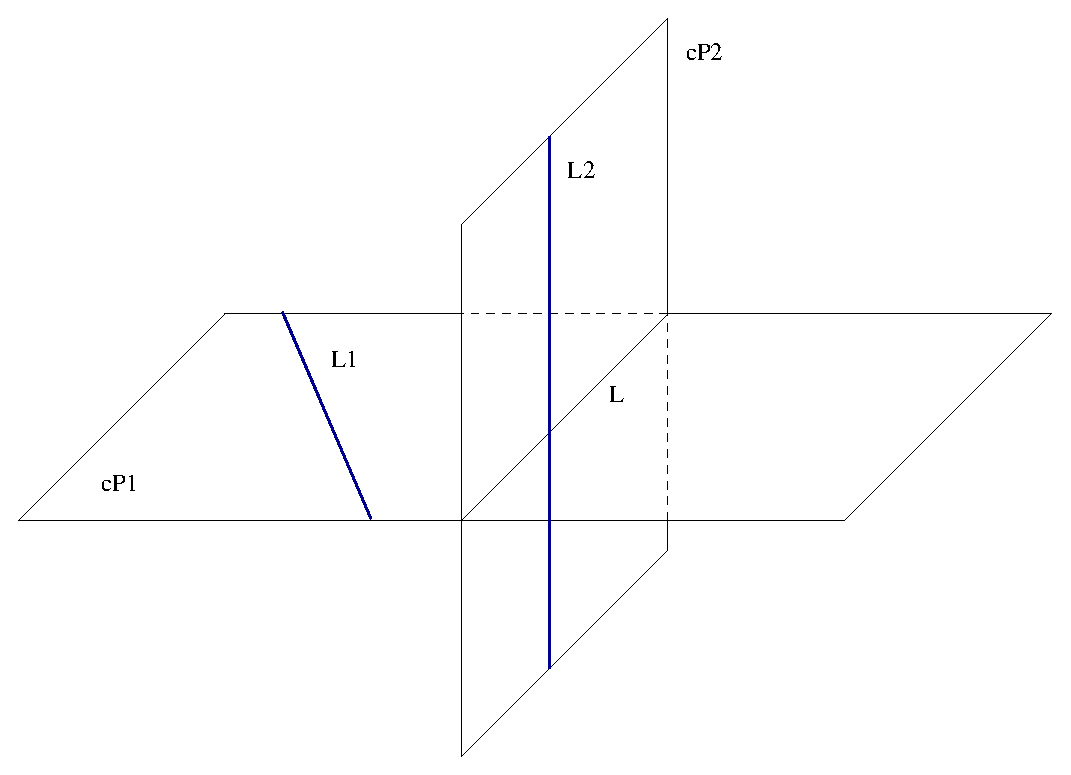
\includegraphics[height=2in]{../../modules/coordinate-systems/pictures/perpendicularity.eps}
  %\caption{Perpendicularity}
  \label{fig:perpendicularity}
\end{figure}
%
\begin{itemize}
%
\item The planes $\mathcal{P}_1$ and $\mathcal{P}_2$ are perpendicular on each other;
%
\item The lines $L_2$ and $L$ are coplanar and perpendicular on each other;
%
\item The lines $L_1$ and $L_2$ are skew but perpendicular on each other;
%
\item The lines $L_1$ and $L$ are coplanar and not perpendicular;
%
\item The line $L_2$ is perpendicular to the plane $\mathcal{P}_1$;
%
\item The line $L_1$ is not perpendicular to the plane $\mathcal{P}_2$.
\end{itemize}

\end{frame}
%\begin{comment}
\begin{frame}
\frametitle{Rectangular/Cartesian Coordinates}
\begin{columns}[T]
\column{0.3\textwidth}
\psset{xunit=0.7cm, yunit=0.7cm}
\begin{pspicture}(-0.5 ,-2)(4.5, 4)
\fcBoundingBox{-0.5}{-2}{4.5}{4}
\tiny
\uncover<3->{
\fcLineIIId{[0 0 0]}{[3 0 0]}
\fcLineIIId{[0 0 0]}{[0 3 0]}
\fcLineIIId{[0 0 0]}{[0 0 3]}
}
\uncover<4->{
\fcLineIIId[arrows=->]{[0 0 0]}{[3 0 0]}
\fcLineIIId[arrows=->]{[0 0 0]}{[0 3 0]}
\fcLineIIId[arrows=->]{[0 0 0]}{[0 0 3]}
}
\uncover<5->{
\fcPutIIId[t]{[3 0 0]}{\alertNoH{5}{$x$}}
\fcPutIIId[lb]{[0 3 0]}{\alertNoH{5}{$y$}}
\fcPutIIId[b]{[0 0 3]}{\alertNoH{5}{$z$}}
}
\uncover<2->{ %
\fcPutIIId[r]{[0 0 0]}{$O~~~$} %
\fcDotIIId[linecolor=black]{[0 0 0]} %
}
\end{pspicture}


\vfill
\column{0.7\textwidth}
\begin{itemize}
\item<1-> A Cartesian coordinate system is given by fixing:
\begin{itemize}
\item<2-> a point $O$ (called the origin),
\item<3-> 3 pairwise perpendicular lines intersecting at the origin,
\item<4-> a direction in each of the coordinate axis.
\end{itemize}
\item<5-> The three lines are labeled as $x$-axis, $y$-axis and $z$-axis.
\end{itemize}

\vskip 3cm
\end{columns}


%
\end{frame}

\begin{frame}
\frametitle{Rectangular/Cartesian Coordinates}
\begin{columns}
\column[t]{0.3\textwidth}
\psset{xunit=0.7cm, yunit=0.7cm}
\begin{pspicture}(-0.5 ,-2)(4.5, 4)
\fcBoundingBox{-0.5}{-2}{4.5}{4}
\tiny
\renewcommand{\fcScreen}{[-1 1.1 -0.5] 0}
\fcAxesIIId{3}{3}{3}
\fcPutIIId[r]{[0 0 0]}{$O~$}
\fcPutIIId[b]{[2.5 2.5 2.8]}{$P(x_P,y_P,z_P)$}
\uncover<9->{
\fcLineIIId[linecolor=gray]{[2.5 2.5 2.5]}{[2.5 2.5 0]}
\fcLineIIId[linecolor=gray]{[2.5 2.5 2.5]}{[2.5 0 2.5]}
\fcLineIIId[linecolor=gray]{[2.5 2.5 2.5]}{[0 2.5 2.5]}
\fcLineIIId[linecolor=gray]{[0 2.5 2.5]}{[0 0 2.5]}
\fcLineIIId[linestyle=dashed, linecolor=gray]{[0 2.5 2.5]}{[0 2.5 0]}
\fcLineIIId[linecolor=gray]{[2.5 0 2.5]}{[0 0 2.5]}
\fcLineIIId[linecolor=gray]{[2.5 0 2.5]}{[2.5 0 0]}
\fcLineIIId[linestyle=dashed, linecolor=gray]{[2.5 2.5 0]}{[0 2.5 0]}
\fcLineIIId[linecolor=gray]{[2.5 2.5 0]}{[2.5 0 0]}%
}%
\fcDotIIId{[2.5 2.5 2.5]}%
\uncover<3-8>{%
\fcPerpendicularIIId{[2.5 2.5 2.5]}{[1 0 0]}{0.3}%
\fcPutIIId[t]{[2.5 0 -0.1]}{$Q$}%
}%
\uncover<4->{\fcPutIIId[t]{[1.25 0 -0.1]}{$x_P$}}%
\uncover<6-8>{%
\fcPerpendicularIIId{[2.5 2.5 2.5]}{[0 1 0]}{0.3}%
\fcPerpendicularIIId{[2.5 2.5 2.5]}{[0 0 1]}{0.3}%
}%
\uncover<6->{%
\fcPutIIId[b]{[0 1.25 0.1]}{$y_P$}%
\fcPutIIId[r]{[0 0 1.25]}{$z_P~~$}%
}
\end{pspicture}


\vfill
\column{0.7\textwidth}
\begin{itemize}
\item<1-> $P$ -point. We assign to it triple $(x_P,y_P,z_P)$.
\item<2-> Assignment will be such that distinct points are assigned distinct triples.
\item<3-> $Q=$ base of perpendicular from $P$ to $x$-axis.
\item<4-> Define $x_P$ as \alertNoH{5}{signed distance b-n $O$ and $Q$}.
\item<5-> Take distance with \alertNoH{5}{$+$ sign if $OQ$ points in direction of $x$-axis, $-$ sign else}.
\item<6-> Definitions of $y_P$, $z_P$ are similar.
\item<7-> $(x_P,y_P,z_P)$ = Cartesian coordinates of $P$. 
\item<8-> $x_P$ is called the $x$-coordinate of $P$,  and so on for other axes.
\item<9-> $(x_P, y_P, z_P)$ = singed lengths of edges of the rectangular box indicated in the picture.
\end{itemize}

\vfill
\end{columns}

\vskip 5cm

\end{frame}
%\end{comment}
\begin{frame}[label=current]
 \frametitle{Euclidean Distance in Coordinates}

   Points $A(x_A,y_A,z_A)$ and $B(x_B,y_B,z_B)$:
   %
\begin{figure}[h]
  \psfrag{O}{$O$}
  \psfrag{A}{$A$} 
  \psfrag{B}{$B(x_B, y_B, z_B)$}  
  \psfrag{C}{$C(x_B, y_B, z_A)$}    
  \psfrag{x}{$y$} 
  \psfrag{y}{$x$} 
  \psfrag{z}{$z$}     
  \psfrag{dx}{$y_B - y_A$}
  \psfrag{dy}{$x_B - x_A$}
  \psfrag{dz}{$z_B - z_A$}  
  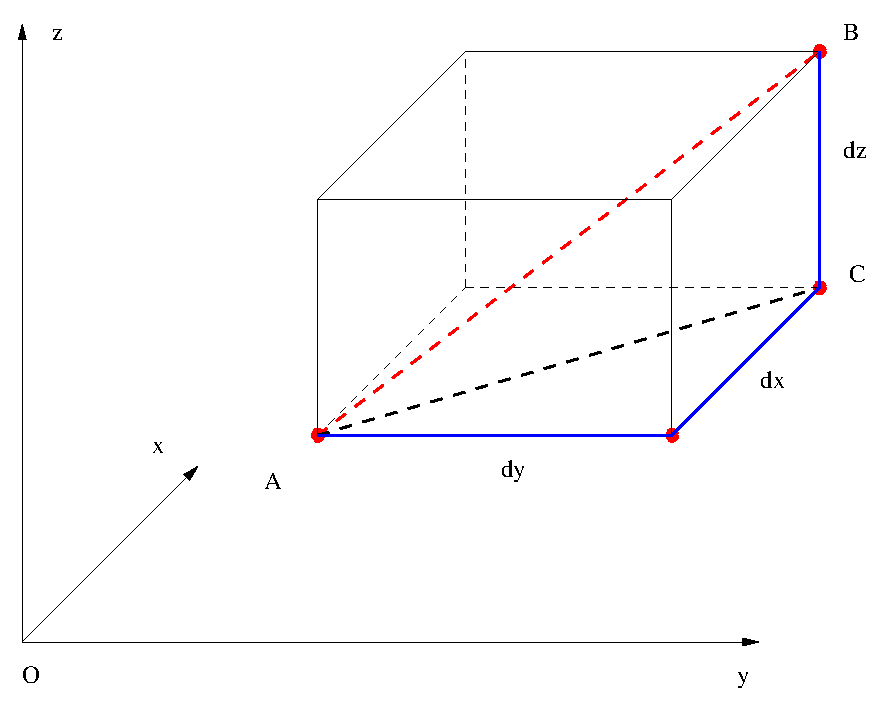
\includegraphics[height=2in]{./images/euclidean_distance.eps}
  %\caption{Euclidean distance}
  %\label{fig:euclidean_distance}
\end{figure}
%
$$d(A,B) = |AB| = \sqrt{(x_B-x_A)^2+(y_B-y_A)^2+(z_B-z_A)^2}$$
%
Example: $P(3,1,2)$ and $Q(1,2,3)$:\pause
%
$$D(P,Q) = \sqrt{(1-3)^2+(2-1)^2+(3-2)^2} = \sqrt{6}\; .$$

\end{frame}
\begin{frame}
  \frametitle{Sets in Space}

  $X$ subset of a set $Y$:

  $$X = \{ A \text{ in } Y | A \text{ has property } \mathcal{P} \} \subset Y$$

\pause
Examples  (Fixed point $Q$, fixed $r>0$):

$$X = \{ A \text{ in Space } | d(A,Q) = r \} = S_r(Q)\; ,$$
\pause Sphere of radius $r$ centered at $Q$.\pause

$$B_r(Q) = \{ A \text{ in Space } | d(A,Q) <r \} \; ,$$
\pause  Open ball of radius $r$ centered at $Q$. \pause

$$\overline{B}_r(Q) = \{ A \text{ in Space } | d(A,Q) \leqslant r\} \; ,$$
\pause  Closed ball of radius $r$ centered at $Q$.

\end{frame}
\begin{frame}
 \frametitle{Equation(s) of Subsets}

  $$X = \{ (x,y,z) | x,y,z \text{ satisfy certain relation(s) } \} \; .$$

\pause
Examples:

$\{(x,y,z) | x^2+y^2+z^2 = 1\}$:

\pause
sphere of radius $r=1$ centered at the origin $(0,0,0)$

Also refered to as: sphere $x^2+y^2+z^2 = 1$

\pause
\medskip

$\{ (x,y,z) | x=0 \}$: coordinate Left-Up plane

\pause
\medskip

$\{ (x,y,z) | x=0 \text{ and } y=0 \}$:

intersection of coordinate planes $\rightarrow$ coordinate axis

\pause
\medskip

Can be given by only one equation:

$x^2+y^2 = 0$ $\rightarrow$ $x=0$,$y=0$, and $z$ arbitrary $\rightarrow$

vertical axis above $(0,0)$ in $(x,y)-$plane

\pause
\medskip

Important: Equations in Plane vs. Space.

\end{frame}
\begin{frame}
 \frametitle{Recognizing Spheres from Equations}

  $Q(x_0,y_0,z_0)$, $r>0$, $A(x,y,z)$. Remark: $d(A,Q) = r \longleftrightarrow d^2(A,Q) = r^2$

$$S_r(Q): \quad (x-x_0)^2+(y-y_0)^2+(z-z_0)^2 = r^2$$

\pause
Example:
$$(x-2)^2+(y-0)^2+(z+1)^2=3^2$$
%
$$x^2+y^2+z^2 -4x + 2z -4=0$$

\pause
\begin{itemize}
 \item no mixed terms $xy$, $xz$, or $yz$;
 \item quadratic terms $x^2$, $y^2$, and $z^2$ with the same coefficient.
\end{itemize}

\pause
Examples:
$$x^2+y^2+z^2-4x+2y=0$$
%
\pause
Complete the square:
%
$$(x-2)^2 + (y+1)^2 +z^2 = 5$$
%
Sphere of radius $\sqrt{5}$ centered at $(2,-1,0)$.

\pause
How about $x^2+y^2+z^2 - 4x+2y = -6$? \pause Passes both tests, but ...
%
$$(x-2)^2 + (y+1)^2 +z^2 = -1$$
%
is impossible! No such points, set is empty.

\end{frame}
}

% begin lecture
\lect{2014}{Lecture  2}{2}{
\section{Vectors}
%\begin{frame}
 \frametitle{Vectors}

\begin{itemize}
 \item Location of projector from current position and orientation:

\pause
\begin{itemize}
  \item direction of projector
  \item distance to projector
\end{itemize}

\pause
\item (direction, distance=magnitude) $\Longleftrightarrow$ \textit{vector}

\pause
\item Examples:
\begin{itemize}
  \item Force
  \item Velocity
  \item Displacement
\end{itemize}
\end{itemize}

\end{frame} %<-needs rewrite from ground up.
\begin{frame}
\frametitle{Definition of vector}
%\begin{pspicture}(-2,-2)(2,2)

%\end{pspicture}

\begin{columns}
\column{0.3\textwidth}
\centering
\begin{pspicture}(-0.2,-0.3)(1.1,1.1)
\fcBoundingBox{-0.2}{-0.3}{1.1}{1.1}
\fcFullDotBlack{0}{0}
\uncover<1-2>{\fcFullDot{1}{1}}
\rput[tl](1.1,0.9){\alert<1>{$\bm v$}}
\rput[t](0,-0.1){\alert<2,4>{$O$}}
\uncover<3>{\psline[arrows=->, linecolor=red](0, 0)(1,1)}
\uncover<4->{\psline[arrows=->](0, 0)(1,1)}
\uncover<4>{\fcFullDot{0}{0}}
\end{pspicture}
\column{0.7\textwidth}
\begin{itemize}
\item A \alert<1>{\emph{position vector $\bm v$}} (simply - \alert<1>{\emph{vector}}) is a point in a space where there's a fixed preferred point $O$.
\item<2-> \alert<2>{Preferred point $O$} is called the \alert<2>{origin}. 
\item<3-> If not given by $O$, vector is depicted by arrow from $O$ to defining point.
\item<4-> Vector given by origin = zero vector $\bm 0$.
\end{itemize}
\end{columns}
\begin{itemize}
\item<5-> Points \& vectors can be identified but:
\begin{itemize}
\item<5-> use term ``vector'' $\Rightarrow$ space has preferred origin point;
\item<7-> if we specifically allow point/vector addition we use the term ``vector'' instead of ``point'';
\item<8-> when we do not intend to carry out addition operations we use the term ``point'' instead of ``vector''.
\end{itemize}
\item<6-> We will soon equip vectors with two operations, vector addition and multiplication by scalars.
\end{itemize}
\end{frame}
\begin{frame}
 \frametitle{Displacement Vectors}

\pause
  Displacement vector = ordered pair of points, $(A,B)$


\begin{itemize}
 \item Represented as an arrow
 \item $A$: tail, $B$: head
 \item Notation: $(A,B) = \overrightarrow{AB} = \textbf{AB}$
  \item Magnitude: $|\textbf{AB}| = |\overrightarrow{AB}|$. 
  \item Direction: Geometric direction from $A$ to $B$, if $A\neq B$ 
  \item If $A=B$:
  \begin{itemize}
    \item Zero magnitude and non-specified direction
    \item $(A,A) = \overrightarrow{AA} = \textbf{AA}$: zero displacement vector.
  \end{itemize}
  \item Displacement vector with tail fixed at $O$:
  \begin{itemize}
    \item Position vector with respect to $O$;
    \item $(O,P) = \overrightarrow{OP} = \textbf{OP} = \textbf{r}_P$.
  \end{itemize}
\end{itemize}

\end{frame}
\begin{frame}
\frametitle{Equality and Equivalence of Displacement Vectors}
\begin{itemize}
\item<1-> We define two displacement vectors $(A,B)$ and $(D,C)$ to be equal if $A=D$ and $B=C$.
\item<2-> Equal displacement vectors $\rightarrow$ same magnitude and direction.
\item<3-> Same magnitude and direction $\not\rightarrow$ equal displacement vectors. 

\item<4-> We define two displacement vectors to be \alertNoH{4}{equivalent} if they have the \alertNoH{4}{same magnitude and direction}. We write $\alertNoH{4}{(A,B) \equiv (D,C)}$.
\item<5-> 
\[ 
(A, B) \equiv (D,C) \Longleftrightarrow ABCD \text{ is a parallelogram}\;.
\]
\end{itemize}
\end{frame}
\begin{comment}
\begin{frame}
\frametitle{Position vectors via displacement vectors}
\begin{itemize}
\item<1-> Suppose we have space without chosen origin.
\item<2-> To each displacement vector $(A,B)$, \uncover<3->{assign \alert<3>{position vector} by choosing \alert<3>{origin to be the tail $A$} and giving the position vector by the head $B$.}
\item<4-> We are ready to give ``origin-free'' alternative definition/interpretation of vector.
\end{itemize}
\uncover<4->{
\begin{definition}[Alternative definition/interpretation of position vector]
Define a position vector as the set that consists all displacement vectors equivalent to one fixed displacement vector.
\end{definition}
}
\begin{columns}
\column{0.15\textwidth}
\psset{xunit=1cm, yunit=1cm}
\begin{pspicture}(-0.4,-0.4)(2, 1.3)
\fcBoundingBox{-0.4}{-0.4}{2}{1.3}
\uncover<2->{\fcFullDot[linecolor=gray]{0}{0}}
\uncover<3->{\fcFullDot[linecolor=red]{0}{0}}
\uncover<2->{
\rput[tl](1, 0.9){$B$}
\rput[tl](0,-0.1){$\alert<3>{ A\uncover<3->{=O}}$}
\fcFullDot[linecolor=gray]{1}{1}
\psline[arrows=->](0,0)(1,1)
}
\end{pspicture}
\column{0.85\textwidth}
\begin{itemize}
\item<5-> Definitions are technically different but equivalent.  \item<6-> We choose which def. to use according to application.
\item<7-> The set of zero displacement vectors with arbitrary tail points = zero  position vector, $\textbf{0}$. 
\end{itemize}
\end{columns}
\end{frame}
\end{comment}
\begin{frame}
\frametitle{Additional notation for position vectors}
\begin{itemize}
\item In preceding slide: each position vector $\bm u$ can be thought of as a set of equivalent displacement vectors.
\item<2-> So we can represent position vectors via displacement vectors.
\item<3-> For two points $A, B$ define the position vector $\overrightarrow{AB}$ or $\bm {AB}$ as the vector represented by the displacement vector $(A,B)$.
\item<4-> $\Rightarrow$ it's allowed to represent position vectors as arrows with tails not necessarily at origin.
%\item<5->  We write $\bm {AB}= \bm{CD}=\bm u$.
\end{itemize}
\begin{figure}
\begin{pspicture}(-1, -2)(2,2)
\fcBoundingBox{-1}{-2.5}{3}{2}
\uncover<1->{
%\fcFullDot{0}{0}
\psline[arrows=->](0,0)(1,1)
\rput[l](0.5, -0.5){$\bm u\uncover<3->{=\bm {AB}}\uncover<4->{=\bm{CD}}$} 
}
\uncover<2->{
\rput[tl](0,-0.1){$A$}
\rput[tl](1,0.9){$B$}
}
\uncover<4->{
%\fcFullDot[lin]{1}{0}
\psline[arrows=->](1,0)(2,1)
\rput[lt](1.1, 0){$C$}
\rput[lt](2, 0.9){$D$}
}
\end{pspicture}
\end{figure}
\end{frame}
\begin{frame}
\frametitle{Addition of Vectors}
\begin{columns}
\column{0.25\textwidth}
\psset{xunit=1cm, yunit=1cm}
\begin{pspicture}(-0.5,-0.5)(3.1,3.1)%
\tiny
\fcBoundingBox{-0.5}{-0.5}{3.1}{3.1}
\uncover<1>{\psline[arrows=->](0,0)(1,2)}
\uncover<1>{%
\rput[r](0.4, 1){$\fcv v$}%
}
\psline[arrows=->](0, 0)(2, 1)%
\rput[t](1, 0.4){$\fcv u$}%
\uncover<2>{
\psline[linecolor=gray, arrows=->](0, 0)(1, 2)%
}
\uncover<2->{%
\psline[arrows=->](2,1)(3,3)%
\rput[l](2.6, 2){$\fcv v$}}
\uncover<3->{%
\psline[arrows=->](0,0)(3,3)
\rput[rb](1.4,1.5){$\fcv u+\fcv v$}
}
\end{pspicture}

\column{0.75\textwidth}
\begin{itemize}
\item<1-> \textbf{Triangle Rule.} Define sum of position vectors $\fcv u$ and $\fcv v$ as follows. 
\item<2-> Attach representative displacement vectors head to tail.
\item<3-> Declare the sum to be the position vector with the tail of the first displacement vector and the head of the second displacement vector.
\end{itemize}
\end{columns}
\end{frame}
\begin{frame}
\frametitle{Properties of addition}
\begin{columns}
\column{0.4\textwidth}
\psset{xunit=1cm, yunit=1cm}
\begin{pspicture}(-0.5,-0.5)(3.1,3.1)%
\tiny
\fcBoundingBox{-0.5}{-0.5}{3.1}{3.1}
\uncover<2-4>{\psline[arrows=->, linecolor=red](0,0)(1,2)}
\uncover<5->{\psline[arrows=->](0,0)(1,2)}
\uncover<2->{\rput[r](0.4, 1){$\alertNoH{2-4}{\fcv v}$}}
\psline[arrows=->](2,1)(3,3)%
\uncover<1>{\psline[arrows=->, linecolor=red](2,1)(3,3)}
\rput[l](2.6, 2){$\alertNoH{1}{\fcv v}$}

\psline[arrows=->](0, 0)(2, 1)%
\uncover<1>{\psline[arrows=->, linecolor=red](0, 0)(2, 1)}
\rput[t](1, 0.4){$\alertNoH{1}{\fcv u}$}%
\uncover<3,4>{\psline[arrows=->, linecolor=red](1,2)(3,3)}
\uncover<5->{\psline[arrows=->](1,2)(3,3)}
\uncover<3->{\rput[b](2, 2.6){$\alertNoH{3,4}{\fcv u}$}}
\psline[arrows=->](0,0)(3,3)
\uncover<1,4>{
\psline[arrows=->, linecolor=red](0,0)(3,3)
}
\uncover<4->{\rput[t](1.62,1.62){\rotatebox{45}{$\alertNoH{4}{ \fcv v+\fcv u}$}}}
\rput[b](1.38,1.38){\rotatebox{45}{$\alertNoH{1}{\fcv{u}+\fcv{v}}$}}
\end{pspicture}

\uncover<5->{
\psset{xunit=0.8cm, yunit=0.8cm}
\begin{pspicture}(-0.5, -1)(4, 4)
\fcBoundingBox{-0.5}{-1}{4}{4}
\tiny

\uncover<5->{\psline[arrows=->](0,0)(0.5, 2) }
\uncover<6,9>{\psline[arrows=->, linecolor=red](0,0)(0.5,2)}
\rput[r](0.15,1){$\alertNoH{6,9}{\fcv{u}}$}

\uncover<5->{\psline[arrows=->](0.5, 2)(3, 3)}
\uncover<6,8>{\psline[arrows=->, linecolor=red](0.5,2)(3,3)}
\rput[b](1.75,2.6){$\alertNoH{6,8}{\fcv v}$}

\uncover<6->{\rput[tl](1.7, 1.7){\alertNoH{6,7}{$\fcv {u}+\fcv {v}$}}}
\uncover<6,7>{\psline[arrows=->, linecolor=red](0,0)(3,3)}
\uncover<8->{\psline[arrows=->](0,0)(3,3)}

\uncover<7>{\psline[arrows=->, linecolor=red](3,3)(4,0)}

\uncover<5->{\psline[arrows=->](3, 3)(4, 0)}
\uncover<7,8>{\psline[arrows=->, linecolor=red](3, 3)(4, 0)}
\rput[lb](3.6,1.5){$\alertNoH{7,8}{\fcv w}$}

\uncover<7->{\rput[t](2, -0.1){\alertNoH{6,7,10}{$(\fcv u+\fcv v )+\fcv w$}}}
\uncover<9->{\rput[b](2, 0.1){\alertNoH{9,10}{$\fcv u+(\fcv v +\fcv w)$}}}
\uncover<8,11->{\psline[arrows=->](0, 0)(4, 0)}
\uncover<7,9,10>{\psline[arrows=->, linecolor=red](0, 0)(4, 0)}


\uncover<8->{\rput[tr](2.25, 1){$\alertNoH{8,9}{\fcv v+\fcv w}$}}
\uncover<10->{\psline[arrows=->](0.5, 2)(4,0)}
\uncover<8,9>{\psline[arrows=->, linecolor=red](0.5, 2)(4,0)}

\end{pspicture}
}
\column{0.6\textwidth}
\begin{itemize}
\item Addition is commutative (parallelogram rule): \[ \alertNoH{1}{\fcv{u}+ \fcv{v}} = \alertNoH{4}{\alertNoH{2}{\fcv{v}}+ \alertNoH{3}{\fcv{u}}}.\]

\item<5-> Addition is associative: 
\[
\alertNoH{10}{\alertNoH{7}{(\alertNoH{6}{ \fcv{u}+\fcv{v}})+\fcv{w} } = \alertNoH{9}{\fcv{u} + (\alertNoH{8}{ \fcv{v} + \fcv{w}})}}
\] 

\item<11-> As usual we write $\fcv{u}+\fcv{v}+\fcv{w}=( \fcv{u} +\fcv{v})+\fcv{w}= \fcv{u}+(\fcv{v}+\fcv{w})$.
\end{itemize}
\end{columns}
\end{frame}


\begin{frame}\frametitle{Difference of vectors}
\begin{columns}
\column{0.4\textwidth}
\psset{xunit=1cm, yunit=1cm}
\begin{pspicture}(-0.5,-2.5)(4.1,3.1)%
\fcBoundingBox{-0.5}{-2.5}{4.1}{3.1}
\uncover<1,2,6>{\rput[b](1, 0.6){$\fcv u$}}
\uncover<1,2,6>{\psline[arrows=->](0,0)(2,1)}
\uncover<3>{\psline[arrows=->, linecolor=red](0,0)(2,1)}

\uncover<3-4,7->{\psline[arrows=->, linecolor=red](2,1)(0,0)}
\uncover<5>{\psline[arrows=->](2,1)(0,0)}
\uncover<3-5,7->{\rput[lt](1,0.5){$\alertNoH{3}{ \alertNoH{4,7}{-\fcv u}\uncover<3>{ =\fcv{BA}}}$}}
\uncover<3>{\fcFullDot{0}{0}}
\uncover<6>{\psline[arrows=->](0,0)(1,-2)}
\uncover<7>{\psline[arrows=->, linecolor=red](0,0)(1,-2)}
\uncover<6->{\rput[tr](0.5, -1){$\alertNoH{7}{\fcv v}~$}}
\uncover<1-5>{%
\rput[tr](0,-0.1){$A$}
\rput[tl](2,0.9){$B$}
}%
\uncover<7->{%
\psline[arrows=->, linecolor=red](2,1)(1,-2)
\rput[l](1.5,-0.5){$~~\alertNoH{7}{\fcv v-\fcv u }$}
}
\end{pspicture}
\column{0.6\textwidth}
\begin{itemize}
\item Let $\fcv u=\fcv{AB}$. 
\item<2-> We define $-\fcv u$ to be \uncover<5->{\alertNoH{5}{the}} \uncover<handout:0|1-4>{a} vector for which $\fcv u +(-\fcv u)=\fcv 0 $. 
\item<3-> Since $\fcv{AB} + \fcv{BA} = \fcv{0}$, it follows $\alertNoH{3}{-\fcv u=\fcv {BA}}$.
\item<4-> In other words $-\fcv{u}$ is depicted using the arrow opposite to $\fcv u$.
\item<5-> From picture, it's evident \alertNoH{5}{$-\fcv u $ can be chosen one way only}.
\item<6-> We define the difference of vectors $\fcv v, \fcv u$ via \uncover<7->{$\alertNoH{7}{\fcv{v}-\fcv{u}= (-\fcv{u})+ \fcv{v} } $ (triangle rule).}
\end{itemize}
\end{columns}
\end{frame}
\begin{frame}
\frametitle{Linear Combinations}
\begin{columns}
\column{0.3\textwidth}
\psset{xunit=0.6cm, yunit=0.6cm}
\begin{pspicture}(-2,-2)(3,3)
\fcBoundingBox{-2}{-2}{3}{3}
\fcFullDot{0}{0}
\rput[br](3, 3){$\fcv u$}
\psline[arrows=->](0,0)(3,3)
\uncover<handout:0|3>{
\psline[arrows=->, linecolor=red](0,0)(1.5,1.5)
\rput[tl](0.75, 0.75){$\alertNoH{3}{\frac{1}{2}\fcv u}$}
}
\uncover<4>{
\psline[arrows=->, linecolor=red](0,0)(2,2)
\rput[tl](1, 1){$\alertNoH{4}{\frac{2}{3}\fcv u}$}
}
\uncover<handout:0|5>{
\psline[arrows=->, linecolor=red](0,0)(1,1)
\rput[tl](0.5, 0.5){$\alertNoH{5}{\frac{1}{3}\fcv u}$}
}
\uncover<6>{
\psline[arrows=->, linecolor=red](0,0)(-2,-2)
\rput[tl](-1, -1){$\alertNoH{6}{-\frac{1}{2}\fcv u}$}
}
\end{pspicture}
\column{0.7\textwidth}
\begin{itemize}
\item<1-> Let $\fcv{u}$ be vector, $c$ be a real number (scalar).
\item<2-> Define \alertNoH{2}{the product of the vector $\fcv u$ and the scalar $c$} as follows.
\begin{itemize}
\item<2-> If $c >0$ define $c\fcv{u}$ as the vector:
\begin{itemize}
\item with the same direction
\item with magnitude proportional with coefficient $c$ to the magnitude of $\fcv u$, i.e., $|c\fcv{u}| = c|\fcv{u}|$.
\end{itemize}

\item<6-> If $c<0$ define $c\fcv{u}$ as the vector $(-c)(-\fcv{u})$, i.e, as the vector:
\begin{itemize}
\item with opposite direction
\item with magnitude $|c\fcv{u}| = |(-c)(-\fcv{u})| = (-c)|-\fcv{u}| = |c||\fcv{u}|$
\end{itemize}
\item<7-> If $c=0$ then define $c\fcv u=0\fcv{u} = \fcv{0}$.
\end{itemize}
\end{itemize}
\end{columns}
\begin{itemize}
\item If $c_1, \ldots , c_n$ are scalars and $\fcv{u}_1,\ldots, \fcv{u}_n$ are vectors, we say
\[
\fcv{v} = c_1\fcv{u}_1+ \dotsb + c_n \fcv{u}_n
\]
is a \emph{linear combination} of the vectors $\fcv u_1,\dots, \fcv u_n$.
\end{itemize}
\end{frame}
%\begin{frame}
  \frametitle{Decomposition of a vector along given directions}

  Example: Tension induced by given force.

\begin{figure}[h]
  \psfrag{F}{$\textbf{F}$}
  \psfrag{-F}{$-\textbf{F}$}
  \psfrag{F1}{$\textbf{F}_1$}
  \psfrag{F2}{$\textbf{F}_2$}
  \psfrag{T1}{$\textbf{T}_1$}
  \psfrag{T2}{$\textbf{T}_2$}
  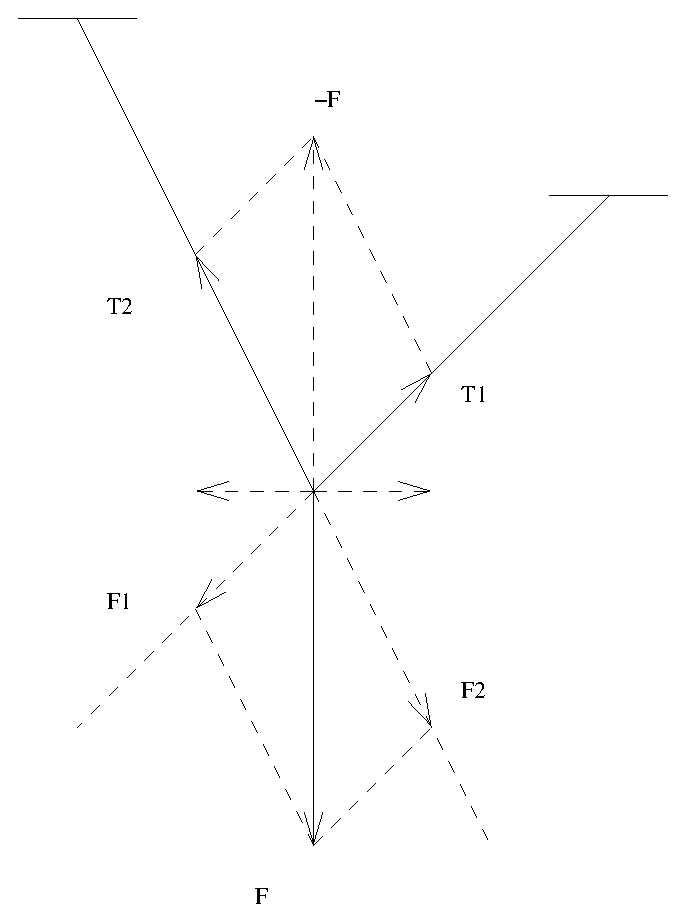
\includegraphics[height=2in]{../../modules/vectors/pictures/ok-tension.eps}
  \label{fig:tension}
  %\caption{Decomposition of a vector}
\end{figure}


\end{frame} %<-slide needs rewrite from ground up.
%\begin{comment}
\begin{frame}
\frametitle{Rectangular/Cartesian Coordinates}
\begin{columns}[T]
\column{0.3\textwidth}
\psset{xunit=0.7cm, yunit=0.7cm}
\begin{pspicture}(-0.5 ,-2)(4.5, 4)
\fcBoundingBox{-0.5}{-2}{4.5}{4}
\tiny
\uncover<3->{
\fcLineIIId{[0 0 0]}{[3 0 0]}
\fcLineIIId{[0 0 0]}{[0 3 0]}
\fcLineIIId{[0 0 0]}{[0 0 3]}
}
\uncover<4->{
\fcLineIIId[arrows=->]{[0 0 0]}{[3 0 0]}
\fcLineIIId[arrows=->]{[0 0 0]}{[0 3 0]}
\fcLineIIId[arrows=->]{[0 0 0]}{[0 0 3]}
}
\uncover<5->{
\fcPutIIId[t]{[3 0 0]}{\alertNoH{5}{$x$}}
\fcPutIIId[lb]{[0 3 0]}{\alertNoH{5}{$y$}}
\fcPutIIId[b]{[0 0 3]}{\alertNoH{5}{$z$}}
}
\uncover<2->{ %
\fcPutIIId[r]{[0 0 0]}{$O~~~$} %
\fcDotIIId[linecolor=black]{[0 0 0]} %
}
\end{pspicture}


\vfill
\column{0.7\textwidth}
\begin{itemize}
\item<1-> A Cartesian coordinate system is given by fixing:
\begin{itemize}
\item<2-> a point $O$ (called the origin),
\item<3-> 3 pairwise perpendicular lines intersecting at the origin,
\item<4-> a direction in each of the coordinate axis.
\end{itemize}
\item<5-> The three lines are labeled as $x$-axis, $y$-axis and $z$-axis.
\end{itemize}

\vskip 3cm
\end{columns}


%
\end{frame}

\begin{frame}
\frametitle{Rectangular/Cartesian Coordinates}
\begin{columns}
\column[t]{0.3\textwidth}
\psset{xunit=0.7cm, yunit=0.7cm}
\begin{pspicture}(-0.5 ,-2)(4.5, 4)
\fcBoundingBox{-0.5}{-2}{4.5}{4}
\tiny
\renewcommand{\fcScreen}{[-1 1.1 -0.5] 0}
\fcAxesIIId{3}{3}{3}
\fcPutIIId[r]{[0 0 0]}{$O~$}
\fcPutIIId[b]{[2.5 2.5 2.8]}{$P(x_P,y_P,z_P)$}
\uncover<9->{
\fcLineIIId[linecolor=gray]{[2.5 2.5 2.5]}{[2.5 2.5 0]}
\fcLineIIId[linecolor=gray]{[2.5 2.5 2.5]}{[2.5 0 2.5]}
\fcLineIIId[linecolor=gray]{[2.5 2.5 2.5]}{[0 2.5 2.5]}
\fcLineIIId[linecolor=gray]{[0 2.5 2.5]}{[0 0 2.5]}
\fcLineIIId[linestyle=dashed, linecolor=gray]{[0 2.5 2.5]}{[0 2.5 0]}
\fcLineIIId[linecolor=gray]{[2.5 0 2.5]}{[0 0 2.5]}
\fcLineIIId[linecolor=gray]{[2.5 0 2.5]}{[2.5 0 0]}
\fcLineIIId[linestyle=dashed, linecolor=gray]{[2.5 2.5 0]}{[0 2.5 0]}
\fcLineIIId[linecolor=gray]{[2.5 2.5 0]}{[2.5 0 0]}%
}%
\fcDotIIId{[2.5 2.5 2.5]}%
\uncover<3-8>{%
\fcPerpendicularIIId{[2.5 2.5 2.5]}{[1 0 0]}{0.3}%
\fcPutIIId[t]{[2.5 0 -0.1]}{$Q$}%
}%
\uncover<4->{\fcPutIIId[t]{[1.25 0 -0.1]}{$x_P$}}%
\uncover<6-8>{%
\fcPerpendicularIIId{[2.5 2.5 2.5]}{[0 1 0]}{0.3}%
\fcPerpendicularIIId{[2.5 2.5 2.5]}{[0 0 1]}{0.3}%
}%
\uncover<6->{%
\fcPutIIId[b]{[0 1.25 0.1]}{$y_P$}%
\fcPutIIId[r]{[0 0 1.25]}{$z_P~~$}%
}
\end{pspicture}


\vfill
\column{0.7\textwidth}
\begin{itemize}
\item<1-> $P$ -point. We assign to it triple $(x_P,y_P,z_P)$.
\item<2-> Assignment will be such that distinct points are assigned distinct triples.
\item<3-> $Q=$ base of perpendicular from $P$ to $x$-axis.
\item<4-> Define $x_P$ as \alertNoH{5}{signed distance b-n $O$ and $Q$}.
\item<5-> Take distance with \alertNoH{5}{$+$ sign if $OQ$ points in direction of $x$-axis, $-$ sign else}.
\item<6-> Definitions of $y_P$, $z_P$ are similar.
\item<7-> $(x_P,y_P,z_P)$ = Cartesian coordinates of $P$. 
\item<8-> $x_P$ is called the $x$-coordinate of $P$,  and so on for other axes.
\item<9-> $(x_P, y_P, z_P)$ = singed lengths of edges of the rectangular box indicated in the picture.
\end{itemize}

\vfill
\end{columns}

\vskip 5cm

\end{frame}
%\end{comment} %<-this slide is to be covered in the first lecture but I did not manage to cover it.
%\begin{comment}
\begin{frame}
\frametitle{Vectors in Coordinates}
\begin{columns}
\column{0.3\textwidth}
\psset{xunit=0.7cm, yunit=0.7cm}
\begin{pspicture}(-0.5 ,-2)(4.9, 4)
\fcBoundingBox{-0.5}{-2}{4.5}{4}
\tiny
\renewcommand{\fcScreen}{[-1 1.1 -0.5] 0}
\fcAxesIIId{3}{3}{3}
\fcPutIIId[r]{[0 0 0]}{$O~$}
\uncover<3->{
\fcLineIIId[arrows=->, linecolor=red]{[0 0 0]}{[1 0 0]}
\fcLineIIId[arrows=->, linecolor=red]{[0 0 0]}{[0 1 0]}
\fcLineIIId[arrows=->, linecolor=red]{[0 0 0]}{[0 0 1]}
\fcPutIIId[t]{[0.5 0 -0.1]}{$\alertNoH{3}{\fcv i}$}
\fcPutIIId[br]{[0 0.5 0]}{$\alertNoH{3}{\fcv j}$}
\fcPutIIId[r]{[0 0 0.5]}{$\alertNoH{3}{\fcv k}~~$}
}
\uncover<5->{
\fcPutIIId[lb]{[2.5 2.5 2.8]}{$U\uncover<6->{(a,b,c)}$}
\fcDotIIId[linecolor=blue]{[2.5 2.5 2.5]}%
\fcLineIIId[arrows=->, linecolor=red]{[0 0 0]}{[2.5 2.5 2.5]}
}
\uncover<2,3>{
\fcDotIIId{[1 0 0]}
\fcDotIIId{[0 1 0]}
\fcDotIIId{[0 0 1]}
}
\uncover<2>{
\fcPutIIId[t]{[1 0 -0.2]}{\alertNoH{2}{$I$}}
\fcPutIIId[br]{[0 1 0]}{\alertNoH{2}{$J~~$}}
\fcPutIIId[r]{[0 0 1]}{\alertNoH{2}{$K~~$}}
}
\uncover<6,11>{
\fcLineIIId[linecolor=gray]{[2.5 2.5 2.5]}{[2.5 2.5 0]}
\fcLineIIId[linecolor=gray]{[2.5 2.5 2.5]}{[2.5 0 2.5]}
\fcLineIIId[linecolor=gray]{[2.5 2.5 2.5]}{[0 2.5 2.5]}
\fcLineIIId[linecolor=gray]{[0 2.5 2.5]}{[0 0 2.5]}
\fcLineIIId[linestyle=dashed, linecolor=gray]{[0 2.5 2.5]}{[0 2.5 0]}
\fcLineIIId[linecolor=gray]{[2.5 0 2.5]}{[0 0 2.5]}
\fcLineIIId[linecolor=gray]{[2.5 0 2.5]}{[2.5 0 0]}
\fcLineIIId[linestyle=dashed, linecolor=gray]{[2.5 2.5 0]}{[0 2.5 0]}
\fcLineIIId[linecolor=gray]{[2.5 2.5 0]}{[2.5 0 0]}%
}
\uncover<6>{
\fcPutIIId[t]{[1.25 0 -0.1]}{$a$}
\fcPutIIId[b]{[0 1.25 0.1]}{$b$}%
\fcPutIIId[r]{[0 0 1.25]}{$c~~$}%
}
\uncover<8->{
\fcPutIIId[t]{[1.25 0 -0.1]}{$a\fcv{i}$}
\fcLineIIId[arrows=->, linecolor=red]{[0 0 0]}{[2.5 0 0]}
}
\uncover<9->{
\fcLineIIId[arrows=->, linecolor=red]{[2.5 0 0]}{[2.5 2.5 0]}
\fcPutIIId[lt]{[2.5 1.25 0]}{$~b\fcv{j}$}%
}
\uncover<10->{
\fcLineIIId[arrows=->, linecolor=red]{[2.5 2.5 0]}{[2.5 2.5 2.5]}
\fcPutIIId[l]{[2.5 2.5 1.25]}{$~c\fcv{k}$}%
}
\end{pspicture}
\column{0.7\textwidth}
\begin{itemize}
\item<1-> Fix coordinate system $Oxyz$.
\item<2-> Let $I$, $J$, $K$ be the points giving the units on the $x,y,z$ axes as indicated.
\item<3-> Define $\fcv{i}$, $\fcv{j}$, $\fcv{k}$ to be the unit vectors $\fcv{OI}$, $\fcv{OJ}$, $\fcv{OK}$.
\end{itemize}
\end{columns}
\begin{itemize}
\item<5-> Let $\fcv u= \fcv{OU}$ be a vector.
\item<6-> Let $U$ have coordinates $(a,b,c)$.
\item<7-> Then $\fcv u =\alertNoH{10}{ \alertNoH{9}{\alertNoH{8}{ a\fcv{i}}+b\fcv{j}}+c\fcv{k} }$.
\item<8-11> This follows from the point-vector identification.
\end{itemize}
\end{frame}
%\end{comment}
\begin{frame}
\begin{columns}
\column{0.3\textwidth}
\psset{xunit=0.7cm, yunit=0.7cm}
\begin{pspicture}(-0.5 ,-2)(4.5, 4)
\fcBoundingBox{-0.5}{-2}{4.5}{4}
\tiny
\renewcommand{\fcScreen}{[-1 1.1 -0.5] 0}
\fcAxesIIId{3}{3}{3}
\fcPutIIId[r]{[0 0 0]}{$O~$}
\fcLineIIId[arrows=->, linecolor=red]{[0 0 0]}{[1 0 0]}
\fcLineIIId[arrows=->, linecolor=red]{[0 0 0]}{[0 1 0]}
\fcLineIIId[arrows=->, linecolor=red]{[0 0 0]}{[0 0 1]}
\fcPutIIId[t]{[0.5 0 -0.1]}{$\alertNoH{3}{\fcv i}$}
\fcPutIIId[br]{[0 0.5 0]}{$\alertNoH{3}{\fcv j}$}
\fcPutIIId[r]{[0 0 0.5]}{$\alertNoH{3}{\fcv k}~~$}
\fcPutIIId[lb]{[2.5 2.5 2.8]}{$U(a,b,c)$}
\uncover<2->{\fcPutIIId[rb]{[1.25 1.25 1.3]}{$\fcv u( a,b,c)$}}
\fcDotIIId[linecolor=blue]{[2.5 2.5 2.5]}%
\fcLineIIId[arrows=->, linecolor=red]{[0 0 0]}{[2.5 2.5 2.5]}
\fcPutIIId[t]{[1.25 0 -0.1]}{$a\fcv{i}$}
\fcLineIIId[arrows=->, linecolor=red]{[0 0 0]}{[2.5 0 0]}
\fcLineIIId[arrows=->, linecolor=red]{[2.5 0 0]}{[2.5 2.5 0]}
\fcPutIIId[lt]{[2.5 1.25 0]}{$~b\fcv{j}$}%
\fcLineIIId[arrows=->, linecolor=red]{[2.5 2.5 0]}{[2.5 2.5 2.5]}
\fcPutIIId[l]{[2.5 2.5 1.25]}{$~c\fcv{k}$}%
\end{pspicture}
\column{0.7\textwidth}
\begin{itemize}
\item<1-> From preceding: arbitrary vector $\fcv u= \fcv {OU}$ can be decomposed as $\fcv u= a\fcv i+b\fcv j + c\fcv k$, where $(a,b,c)$: Cartesian coordinates of $U$.
\item<2-> Thus $\fcv u$ is identified with the triple of numbers $( a, b, c)$.
\end{itemize}
\end{columns}

\begin{itemize}
\item<3-> Under the first definition of vector, a vector is simply a point in a vector space (=space with a distinguished point).
\item<4-> From now on, we assume the first definition of vector: we use the notation $(a,b,c)$ both for points in vector spaces (vectors) and points in spaces not equipped with vector space structure.
\item<5-> Under the second alternative definition of vector, there is a formal distinction between points and vectors.
\item<6-> Some authors who use the second definition use the notation $\langle a, b, c \rangle$ to denote vectors and $(a,b,c)$ to denote points.
\end{itemize}
\end{frame}

\begin{frame}
\frametitle{Operations in Coordinates}
\begin{itemize}
\item<1-> Vector magnitude is given by 
\[
|\langle a, b, c \rangle| = |OP| = \sqrt{a^2+b^2+c^2}
\]
\item<2-> Vector addition is given by:
\[
\langle x_1,y_1,z_1 \rangle + \langle x_2, y_2,z_2\rangle = \langle x_1+x_2, y_1+y_2, z_1+z_2\rangle\; .
\]
\item<3-> Scalar multiple is given by:
\[
c\langle x, y, z\rangle = \langle cx, cy, cz\rangle\; .
\]
\item<4-> Let $A(x_A, y_A, z_A)$ and $B(x_B, y_B, z_B)$ be points. Then
\[
\bm{AB} = \bm{AO} +\bm{OB} = \bm{OB} - \bm{OA} = \langle x_B-x_A, y_B-y_A, z_B-z_A\rangle \; .
\]
\end{itemize}

\end{frame}
%\begin{frame}
 \frametitle{Work done by a constant force}

\only<1>{
\begin{figure}[h]
  \psfrag{F}{$\textbf{F}$}
  \psfrag{O}{$O$}
  \psfrag{P}{$P$}
  \psfrag{a}{$\alpha$}
  \psfrag{pvF}{$\textbf{proj}_{\bm{v}} \textbf{F}$}
  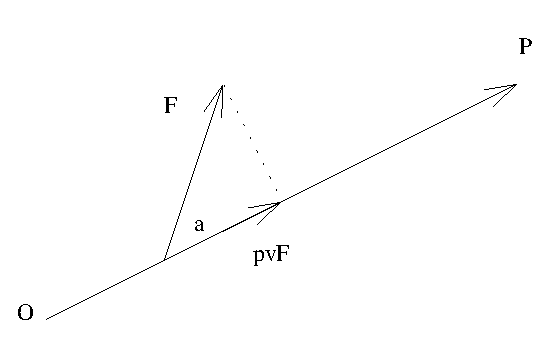
\includegraphics[height=2in]{../../modules/vectors/pictures/ok-positive_work.eps}
\end{figure}

$$W = |\textbf{proj}_{\bm{v}} \textbf{F}| \, |\textbf{OP}| =|\textbf{F}| \, |\textbf{OP}|\, \cos{\alpha}\; .$$
}

\only<2>{
\begin{figure}[h]
  \psfrag{F}{$\textbf{F}$}
  \psfrag{O}{$O$}
  \psfrag{P}{$P$}
  \psfrag{a}{$\alpha$}
  \psfrag{pvF}{$\textbf{proj}_{\bm{v}} \textbf{F}$}
  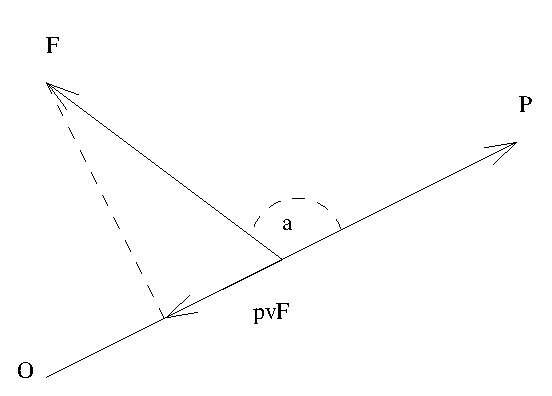
\includegraphics[height=2in]{../../modules/vectors/pictures/ok-negative_work.eps}
\end{figure}

$$W = - |\textbf{proj}_{\bm{v}} \textbf{F}| \, |\textbf{OP}| = |\textbf{F}| |\textbf{OP}| \cos{\alpha}\; .$$
}

\end{frame} %<-needs a ground-up rewrite

\section{Dot product of vectors}
\begin{frame}
\frametitle{Dot Product}
\begin{columns}
\column{0.5\textwidth}
\begin{pspicture}(-2, -0.5)(5,3.2)
\fcBoundingBox{-2}{-0.5}{5}{3.2}%
\psline[arrows=->](0,0)(4, 2)%
\rput[tl](3, 1.5){$\fcv v$}%
\rput[bl](1, 3){$ \fcv u$}%
\uncover<4->{\rput[r](-0.5, 1){$\textbf{orth}_{\fcv v} \fcv u$}}%
\uncover<4->{\fcPerpendicular[linestyle=dashed]{[1 3]}{[-2 4]}{0.2}}%
\uncover<2->{%
\psline[arrows=->, linecolor=blue](0,0)(2,1)%
\rput[tl](1.5, 0.8){$\textbf{proj}_{\fcv v} \fcv u$}%
}%
\uncover<6->{%
\psline[arrows=->, linecolor=red](0,0)(! 4 20 sqrt div 2 20 sqrt div)%
\rput[tl](0.5, 0.2){$\widehat{ \fcv {v}}$}%
}%
\psline[arrows=->](0,0)(1,3)%
\uncover<4->{\psline[arrows=->](0,0)(! -1 2)}%
\uncover<2->{%
\fcPerpendicular[linestyle=dashed]{[1 3]}{[4 2]}{0.2}%
}%
\uncover<6->{\fcAngle{0.463648}{ 1.249046 }{0.4}{$\alpha$}}%
\end{pspicture}
\column{0.5\textwidth}

\begin{itemize}
\item<1-> Let $\fcv{u}$, $\fcv{v}$ vectors, $\fcv{v}\neq \fcv{0}$.

\item<2-> Denote by $\textbf{proj}_{\fcv{v}} \fcv{u}$ the projection of $\fcv{u}$ along $\fcv{v}$.
\item<3-> Denote by $\textbf{comp}_{\fcv{v}}\fcv{u}$ the magnitude of $ \textbf{proj}_{\fcv{v}} \fcv{u}$, i.e.,

$|\textbf{proj}_{\fcv{v}} \fcv{u}|= \textbf{comp}_{\fcv{v}}\fcv{u}
$
\end{itemize}
\end{columns}
\begin{itemize}
\item<4-> Denote by $\textbf{orth}_{\fcv{v}} \fcv{u}$ the projection of $\fcv{u}$ in direction orthogonal to $\fcv{v}$.
\item<5-> $\fcv u = \textbf{orth}_{\fcv v}\fcv u + \textbf{proj}_{\fcv v} \fcv u$.

\item<6-> We have $\widehat{\fcv{v}} = \frac{1}{|\fcv{v}|} \fcv{v}$ is the unit vector along $\fcv{v}$.

%NOTE we need to use the \widehat and not the \hat command BECAUSE \hat is buggy in the present version of beamer and does not display correctly in \[\]-math mode.

\item<7-> Let $\alpha$: angle between $\fcv v$ and $\fcv u$.

\item<8-> Then $\textbf{comp}_{\fcv{v}} \fcv{u} =  \cos \alpha |\fcv{u}|$. \uncover<9-> {Therefore $\textbf{proj}_{\fcv{v}} \fcv{u} =  \cos \alpha |\fcv{u}| \widehat{\fcv{v}}$.}

\item<10-> Define dot product of $\fcv u$ and $\fcv v$:
\[
\fcv{u} \cdot \fcv{v} =  \cos \alpha |\fcv u||\fcv{v}| .
\]
\end{itemize}
\end{frame}

\begin{frame}
 \frametitle{Properties of Dot Product}

  \begin{itemize}
   \item If $\textbf{v}=\textbf{0}$ or $\textbf{u}=\textbf{0}$, then $\textbf{u}\cdot \textbf{v} =0$.

  \item If $\textbf{u} \neq 0 \neq \textbf{v}$, then $comp_{\bm{v}} \textbf{u} = |\textbf{u}|\cos{\alpha}$
%
$$\textbf{u} \cdot \textbf{v} = |\textbf{u}| \, |\textbf{v}|\,\cos{\alpha}$$
%
\item If $\textbf{u}\neq \textbf{0} \neq \textbf{v}$, then
%
$$\textbf{u} \cdot \textbf{v} = 0 \Longleftrightarrow \textbf{u} \bot \textbf{v}\; .$$
%
\item $\textbf{u} \cdot \textbf{v} = (\textbf{proj}_{\bm{v}} \textbf{u}) \cdot \textbf{v}$

\item The dot product is linear in each argument:
%
$$ (a \textbf{u} + b \textbf{w}) \cdot \textbf{v} = a \textbf{u} \cdot \textbf{v} + b \textbf{w} \cdot \textbf{v}$$
%
$$ \textbf{u} \cdot (a \textbf{v} + b \textbf{w}) = a \textbf{u} \cdot \textbf{v} + b \textbf{u} \cdot \textbf{w}$$

\item Dot product is positive definite:
%
$$\textbf{v} \cdot \textbf{v} = |\textbf{v}|^2 \geqslant 0 \text{ and }
\textbf{v}\cdot \textbf{v} = 0 \leftrightarrow \textbf{v}=\textbf{0}$$
  \end{itemize}

\end{frame}
\begin{frame}
 \frametitle{Computations in Coordinates}

 \begin{itemize}
  \item  $Oxyz$: rectangular coordinate system

  \item $\textbf{i}$, $\textbf{j}$, $\textbf{k}$: unit vectors along fundamental directions.
%
$$ \textbf{i} \cdot \textbf{j} = \textbf{j} \cdot \textbf{i} = \textbf{j} \cdot \textbf{k}
 = \textbf{k} \cdot \textbf{j} = \textbf{i} \cdot \textbf{k} = \textbf{k} \cdot \textbf{i} = 0$$
%
$$\textbf{i} \cdot \textbf{i} = \textbf{j} \cdot \textbf{j} = \textbf{k} \cdot \textbf{k} = 1$$

  \item $\textbf{u} = u_1 \textbf{i} + u_2 \textbf{j} + u_3 \textbf{k} = \langle u_1, u_2, u_3 \rangle$,
 $\textbf{v}=v_1 \textbf{i} + v_2 \textbf{j} + v_3 \textbf{k} = \langle v_1, v_2, v_3 \rangle$,
%
$$\textbf{u} \cdot \textbf{v} = \langle u_1, u_2, u_3 \rangle \cdot \langle v_1, v_2, v_3 \rangle =
u_1v_1 + u_2 v_2 +u_3 v_3\; .$$

\item Example: $\langle 1,2,3 \rangle \cdot \langle 6,5,4 \rangle = 1 \cdot 6 + 2\cdot 5 + 3 \cdot 4 = 28$.
 \end{itemize}
\end{frame}

\begin{frame}
\begin{example}
$\alert<2>{\langle 1,2,3 \rangle \cdot \langle 6,5,4 \rangle =} \uncover<3->{\alert<3>{1 \cdot 6 + 2\cdot 5 + 3 \cdot 4 = 28}}$
\end{example}
\end{frame}

\begin{frame}
\begin{example}
\begin{columns}
\column{0.25\textwidth}
\psset{xunit=0.5cm, yunit=0.5cm}
\begin{pspicture}(-2, -2)(3,3)%
\renewcommand{\fcScreen}{[-1 0.8 -0.2] 0}%
\only<6->{\renewcommand{\fcScreen}{[-1 0.571429 -0.2] 0}}
\only<7->{\renewcommand{\fcScreen}{[-1 0.342857 -0.2] 0}}
\only<8->{\renewcommand{\fcScreen}{[-1 0.114286 -0.2] 0}}
\only<9->{\renewcommand{\fcScreen}{[-1  -0.114286 -0.2] 0}}
\only<10->{\renewcommand{\fcScreen}{[-1 -0.342857 -0.2] 0}}
\only<11->{\renewcommand{\fcScreen}{[-1 -0.8 -0.2] 0}}
\fcBoundingBox{-3}{-3}{3}{3}%
\fcAxesIIIdFull{3}{3}{3}%
\uncover<4->{\fcPerpendicularIIId{[1 -2 3]}{[-1 1 1]}{0.4}}%
\fcLineIIId[linecolor=blue,arrows=->]{[0 0 0]}{[1 -2 3]}%
\fcLineIIId[linecolor=blue, arrows=->]{[0 0 0]}{[1 -1 -1]}%
\end{pspicture}
\column{0.75\textwidth}
Are the vectors $\langle 1,-2,3 \rangle \cdot \langle 1,-1,-1 \rangle $ perpendicular?

\[
\uncover<2->{\alert<2,3>{ \langle 1,-2,3 \rangle \cdot \langle 1,-1,-1 \rangle =}} \uncover<3->{\alert<3>{1\cdot 1 + (-1)\cdot (-2)+ 3\cdot (-1)=0}},
\] 
\uncover<4->{therefore the vectors are perpendicular.} 
\uncover<5->{Is this apparent from the picture? Not unless the two vectors lie in a plane parallel to the surface of the page/computer screen.}
\uncover<12>{}
\end{columns}
\end{example}
\end{frame}
\begin{frame}
\frametitle{Projections in coordinates}
\begin{columns}
\column{0.4\textwidth}
\psset{xunit=0.6cm, yunit=0.6cm}
\begin{pspicture}(-2, -0.5)(5,3.2)
\fcBoundingBox{-2}{-0.5}{5}{3.2}%
\psline[arrows=->](0,0)(4, 2)%
\rput[tl](3, 1.5){$\fcv v$}%
\rput[bl](1, 3){$ \fcv u$}%
\psline[arrows=->, linecolor=blue](0,0)(2,1)%
\rput[tl](1.5, 0.8){$\textbf{proj}_{\fcv v} \fcv u$}%
\psline[arrows=->, linecolor=red](0,0)(! 4 20 sqrt div 2 20 sqrt div)%
\rput[tl](0.5, 0.1){$\widehat{ \fcv {v}}$}%
\psline[arrows=->](0,0)(1,3)%
\fcPerpendicular[linestyle=dashed]{[1 3]}{[4 2]}{0.2}%
\end{pspicture}
\column{0.6\textwidth}
\[
\begin{array}{rcl}
\fcv{u} &=& u_1 \fcv{i} + u_2 \fcv{j} + u_3 \fcv{k} = \langle u_1, u_2, u_3 \rangle\\
\fcv{v}&=&v_1 \fcv{i} + v_2 \fcv{j} + v_3 \fcv{k} = \langle v_1, v_2, v_3 \rangle
\end{array}
\]
\end{columns}
\uncover<2->{
\begin{theorem}
$\begin{array}{rcl}
\displaystyle\alert<6>{ {\bf comp}_{\fcv v} \fcv u}&\alert<6>{=}& \displaystyle \alert<6>{\frac{\alert<3>{\fcv{u}\cdot \fcv{v}} }{\alert<4>{|\fcv{v}|}}} =\frac{ \alert<3>{ u_1v_1 +u_2v_2+u_3v_3} }{\alert<4>{ \sqrt{v_1^2+v_2^2+v_3^2}}}\\~\\
\displaystyle \alert<5>{{\bf proj}_{\fcv v} \fcv u }&\alert<-1>{=}&\displaystyle \alert<5>{\left(\alert<6>{ {\bf comp}_{\fcv v} \fcv{u}}\right) \alert<7>{\widehat{\fcv v}}} = \alert<6>{\frac{\fcv{u}\cdot \fcv{v}}{|\fcv{v}|}} \alert<7>{ \frac{\fcv v}{|\fcv v|}} = \frac{\fcv{u}\cdot \fcv{v}}{\alert<8>{ |\fcv{v}|^2}}\fcv v= \frac{\fcv u \cdot \fcv v}{\alert<8>{ \fcv v\cdot  \fcv v} }\fcv v
\quad .
\end{array}
$
\end{theorem}
}
\end{frame}

\begin{frame}
\begin{example}
Let $\fcv u=( 1,2,3)$, $\fcv v=( 6,5,4 )$.
\begin{itemize}
\item Compute the scalar projection $\text{comp}_{\fcv v} \fcv u$ of $\fcv u$ onto $\fcv v$.
\item Compute the vector projection ${\bf proj}_{\fcv v} \fcv u$ of $\fcv u$ onto $\fcv v$.
\item Compute the orthogonal component ${\bf orth}_{\fcv v}\fcv u$.
\end{itemize}

$
\begin{array}{r@{}c@{}l}
\uncover<2->{\displaystyle\text{comp}_{\fcv v}\fcv u&~=~& \displaystyle \frac{\fcv u\cdot \fcv v}{|\fcv v|} \\~\\}
\uncover<2->{\displaystyle\alert<2,3>{ \text{comp}_{( 6,5,4)} ( 1,2,3) }&\alert<2,3>{~=~}& \uncover<3->{\alert<3>{\displaystyle \frac{ (6, 5,4)\cdot(1,2,3)}{\sqrt{( 6, 5, 4 )\cdot ( 6, 5 ,4 )}} = \frac{6\cdot 1 + 5\cdot 2 + 4\cdot 3}{\sqrt{6^2+5^2+4^2}} = \frac{28}{\sqrt{77}}}} \\~\\}
\uncover<4->{ {\bf proj}_{\fcv{v}} \textbf{u} &~=~&\displaystyle \frac{\fcv{u} \cdot \fcv{v}}{|\fcv{v}|^2} \fcv{v}\\~\\}
\uncover<4->{\alert<4,5>{ {\bf proj}_{( 6,5,4)} ( 1,2,3) }& \alert<4,5>{~ =~}&\uncover<5->{\alert<5>{ \frac{28}{77} ( 6,5,4) = \left(\frac{24}{11}, \frac{20}{11}, \frac{16}{11}\right)}} \\}
\uncover<6->{\alert<6,7>{{\bf orth}_{( 6,5,4)} ( 1,2,3)} &\alert<6,7>{~=~}& \uncover<7->{\alert<7>{( 1,2,3) -
\textbf{proj}_{( 6,5,4)} ( 1,2,3)= \left(-\frac{13}{11}, \frac{2}{11}, \frac{17}{11}\right) }}}
\end{array}
$
\end{example}
\end{frame}

\begin{frame}
\frametitle{Angles}
\begin{columns}
\column{0.3\textwidth}
\psset{xunit=0.6cm, yunit=0.6cm}
\begin{pspicture}(-2, -0.5)(5,3.2)
\fcBoundingBox{-2}{-0.5}{5}{3.2}%
\psline[arrows=->](0,0)(4, 2)%
\rput[tl](3, 1.5){$\fcv v$}%
\rput[bl](1, 3){$ \fcv u$}%
\psline[arrows=->, linecolor=blue](0,0)(2,1)%
\psline[arrows=->](0,0)(1,3)%
\fcPerpendicular[linestyle=dashed]{[1 3]}{[4 2]}{0.2}%
\fcAngle{0.463648}{ 1.249046 }{0.4}{$\alpha$}%
\end{pspicture}

Let $\alpha=\angle (\fcv u, \fcv v)$.
\column{0.7\textwidth}
\[
\begin{array}{rcl}
\displaystyle\fcv u \cdot \fcv v& =&\displaystyle |\fcv u||\fcv v|\cos \alpha\\
\uncover<2->{\displaystyle\cos{\alpha} &=&\displaystyle \frac{\textbf{u} \cdot \textbf{v}}{|\textbf{u}|\, |\textbf{v}|} } \\
\uncover<3->{\displaystyle\alpha &=& \displaystyle\arccos{\left( \frac{\textbf{u} \cdot \textbf{v}}{|\textbf{u}|\, |\textbf{v}|} \right)}
}
\end{array}
\]
\end{columns}

\begin{example}
\uncover<4->{
Compute the angle $\angle(\langle 1,2,3\rangle,\langle 6,5,4\rangle)$.}
\uncover<5->{
\[
\begin{array}{rcl}
\alpha &=& \displaystyle \Arccos\left(\frac{\langle1,2,3\rangle \cdot \langle6,5,4\rangle}{|\langle1,2,3\rangle || \langle6,5,4\rangle|} \right)  \\
&=&\displaystyle \Arccos{\left( \frac{28}{\sqrt{14}\, \sqrt{77}} \right)} = \Arccos{\left( \frac{4}{\sqrt{22}} \right)}
\end{array}
\]
}
\end{example}
\end{frame}

\begin{frame}
 \frametitle{Direction Angles}
\begin{definition}
The direction angles $\alpha, \beta, \gamma$ of the vector $\fcv u$ are defined as the angles between $\fcv u $ and the unit vectors $\fcv i, \fcv j, \fcv k$ (in the same order).
\end{definition}
\begin{columns}
\column{0.5\textwidth}
\psset{xunit=2cm, yunit=2cm}
\begin{pspicture}(-2,-2)(2,2)
\renewcommand{\fcScreen}{[-2 -1 -0.6] 0}
\fcAxesIIId{2}{2}{2}
\fcLineIIId[arrows=->, linecolor=red]{[0 0 0]}{[1.5 1.5 1.5]}
\fcLineIIId[arrows=->, linecolor=blue]{[0 0 0]}{[1 0 0]}
\fcLineIIId[arrows=->, linecolor=blue]{[0 0 0]}{[0 1 0]}
\fcLineIIId[arrows=->, linecolor=blue]{[0 0 0]}{[0 0 1]}
\fcAngleIIId[arrows=->, linecolor=brown]{[1 0 0]}{[1.5 1.5 1.5]}{1}%
\fcAngleIIId[arrows=->, linecolor=brown]{[0 1 0]}{[1.5 1.5 1.5]}{1.4}%
\fcAngleIIId[arrows=->, linecolor=brown]{[0 0 1]}{[1.5 1.5 1.5]}{1.8}%
\fcPutIIId[bl]{[0.75 0 0.25]}{$\alpha~~$}
\fcPutIIId[bl]{[0.75 1.25 0.55]}{$~~\beta$}
\fcPutIIId[r]{[1 1 1.6]}{$~~\gamma$}
\end{pspicture}

\column{0.5\textwidth}

$\textbf{u} = ( u_1, u_2, u_3)$

$\alpha = \angle (\textbf{u},\textbf{i})$

$\beta =
\angle (\textbf{u},\textbf{j})$

$\gamma = \angle (\textbf{u},\textbf{k}) \; .$

$$\cos{\alpha} = \frac{\textbf{u} \cdot \textbf{i}}{|\textbf{u}|\, |\textbf{i}|} =
\frac{u_1}{\sqrt{u_1^2+u_2^2+u_3^2}}$$

Similar for $\cos{\beta}$ and $\cos{\gamma}$. Then:
%
$$\cos^2\alpha + \cos^2\beta + \cos^2\gamma = 1\; .$$
\end{columns}
\end{frame}

%\begin{frame}
 \frametitle{Rotational Effect}

 \begin{itemize}
  \item Rigid rod $OP$, fixed at $O$, $\textbf{r}=\textbf{OP}$. Force $\textbf{F}$ applied at $P$.
 \end{itemize}
%
\begin{figure}[h]
  \psfrag{F}{$\textbf{F}$}
  \psfrag{r}{$\textbf{r}$}
  \psfrag{O}{$O$}
  \psfrag{P}{$P$}
  \psfrag{}{$\alpha$}
  \psfrag{pfr}{$\textbf{proj}_{\bm{r}} \textbf{F}$}
  \psfrag{ofr}{$\textbf{orth}_{\bm{r}} \textbf{F}$}
  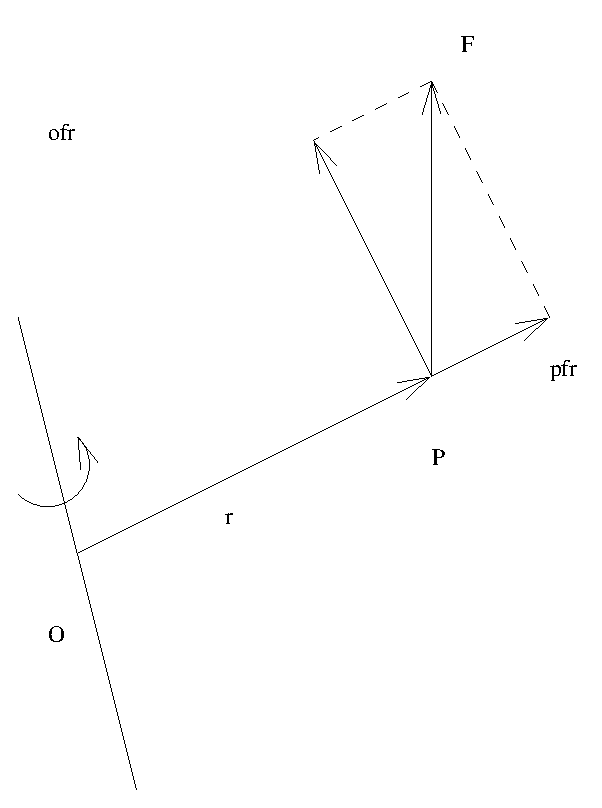
\includegraphics[height=1.5in]{../../modules/vectors/pictures/ok-torque.eps}
\end{figure}
%
\pause
\begin{itemize}
  \item $\textbf{proj}_{\bm{r}} \textbf{F}$: \pause no effect;
  \item $\textbf{orth}_{\bm{r}} \textbf{F}$: \pause rotational effect:\pause
  \begin{itemize}
    \item Axis of rotation: \pause perpendicular to $\textbf{r}$ and $\textbf{F}$;\pause
    \item Angular velocity: \pause proportional to $|\textbf{orth}_{\bm{r}} \textbf{F}|$;\pause
    \item Linear velocity: \pause proportional to $|\textbf{r}| \, |\textbf{orth}_{\bm{r}} \textbf{F}|$.
  \end{itemize}
\end{itemize}

\end{frame} %<-needs to be rewritten from ground up
%\begin{frame}
 \frametitle{Torque}

  Rotation in space $\Longleftrightarrow$ vector\pause
  \begin{itemize}
   \item Axis of rotation $\Longleftrightarrow$ Support of direction \pause
   \item Sense of rotation  $\Longleftrightarrow$ Direction of vector \pause
  \begin{itemize}
      \item Convention: Right Hand Rule\pause
  \end{itemize}
  \item Angular velocity $\Longleftrightarrow$ (proportional to) Magnitude of vector\pause
  \end{itemize}
\begin{center}
 $(\textbf{r}, \textbf{F}) \rightarrow$ rotation $\rightarrow$ vector = torque, $\bm{\tau}$
\end{center}



\begin{itemize}
 \item Support of direction: perpendicular to $\textbf{r}$ and $\textbf{F}$;
 \item Direction: Right Hand Rule;
 \item Magnitude: $|\bm{\tau}| = |\textbf{r}| \, |\textbf{orth}_{\bm{r}} \textbf{F}|$
\end{itemize}

\end{frame} %<-needs to be rewritten from ground up
}

\lect{September 2014}{Lecture 3}{3}{
\section{Cross product of vectors}
\begin{frame}
\frametitle{Torque}
\begin{columns}
\begin{pspicture}(-0.2, -1.2)(2, 1.2)
\tiny%
\fcBoundingBox{-0.2}{-1.2}{2}{1.2}%
\uncover<1-2>{\fcLineIIId{[0 0 -0.2]}{[0 0 -1]}}%
\uncover<3->{\fcLineIIId[arrows=->]{[0 0 -0.2]}{[0 0 -1]}}%
\uncover<3->{\fcLineIIId[arrows=->]{[0 0 1]}{[0 0 0.1]}}%
%\fcAxesIIId{1}{1}{1}
\fcPolyLineIIId{[0.2  0 0.1] [0.1 0.173205 0.1] [-0.1 0.173205 0.1] [-0.2 0 0.1] [-0.1 -0.173205 0.1] [0.1 -0.173205 0.1] [0.2 0 0.1]}%
\fcPolyLineIIId{[-0.1 -0.173205 -0.1] [0.1 -0.173205 -0.1] [0.2 0 -0.1] [0.1 0.173205 -0.1]}%
\fcLineIIId{[-0.1 -0.173205 -0.1]}{[-0.1 -0.173205 0.1]}%
\fcLineIIId{[0.1 -0.173205 -0.1]}{[0.1 -0.173205 0.1]}%
\fcLineIIId{[0.2 0 -0.1]} {[0.2 0 0.1]}%
\fcLineIIId{[0.1 0.173205 -0.1]}{[0.1 0.173205 0.1]}%
\uncover<2->{\fcPolyLineIIId[linecolor=blue]{[0.15 -0.259808 0] [0.3 0 0] [0.15 0.259808 0] [0.04 0.259808 0]}%
\fcLineIIId[linecolor=blue]{[0.15 0.259808 0]}{[0.15 0.259808 0] 5 \fcVectorTimesScalar}%
}%
\uncover<4->{\fcLineIIId[linecolor=blue, arrows=->]{[0.15 0.259808 0]} {[0.15 0.259808 0] 5 \fcVectorTimesScalar}%
\fcPutIIId[b]{[0.32 0.65 0.1]}{$\fcv r$}%
}%
\uncover<3->{\fcAngleIIId[arrows=->, linecolor=blue]{[0.15 0.259808 0]}{[0.4 0.2 0]}{1.2}}%
\uncover<4->{\fcLineIIId[arrows=->, linecolor=red]{[0.75 1.29904 0]}{[1 0.5 1]}}%
\uncover<5->{\fcLineIIId[arrows=->]{[0.75 1.29904 0]}{[0.75 1.29904 1]}
\fcPutIIId[l]{[0.75 1.3 0.5]}{$~~\fcv F_o$}
}%
\uncover<6->{\fcLineIIId[arrows=->]{[0.75 1.29904 0]}{[0.466506 0.808013 0]}%
\fcPutIIId[b]{[0.61 1.05 0]}{$~~\fcv F_\rho$}%
}%
\uncover<7->{\fcLineIIId[arrows=->]{[0.75 1.29904 0]}{[1.283494 0.991027 0]}%
\fcPutIIId[l]{[1 1.15 0]}{$~~\fcv F_\theta$}%
}%
\uncover<9->{\fcPutIIId[r]{[0 0 -0.5]}{$\tau~$}}%
\end{pspicture}

\column{0.7\textwidth}
\begin{itemize}
\item If we tighten a bolt \uncover<2->{using a wrench,} \uncover<3->{it moves in direction perpendicular to the motion of the wrench.}
\item<4-> Let arm of the wrench: given by vector $\fcv r$. 
\end{itemize}
\end{columns}
\begin{itemize}
\item<4-> Suppose we are applying a force $\fcv F$ at arm of the wrench. The force has three components: 
\begin{itemize}
\item<5-> component $\fcv F_o$ orthogonal to the plane of rotation
\item<6-> component $\fcv F_\rho$ in the plane of rotation towards/away from the center
\item<7-> component $\fcv F_\theta$ tangent to the motion of the wrench.
\end{itemize}
\item<8-> Only $\fcv F_\theta$ contributes to the bolt motion.
\item<9-> The force of bolt motion $\fcv \tau$ is proportional to length of wrench.
\item<10-> It turns out $\fcv \tau = \fcv r \times (\fcv F_\rho+\fcv F_\theta)$, where \alert<10>{$\times$ is the vector cross product}.
\end{itemize}
\end{frame}
\begin{frame}
 \frametitle{Cross Product}

\begin{center}
 (\textbf{vector}, \textbf{vector}) $\to$ \textbf{vector}
\end{center}

\begin{figure}[h]
  \psfrag{u}{$\textbf{u}$}
  \psfrag{v}{$\textbf{v}$}
  \psfrag{ovu}{$\textbf{orth}_{\bm{u}} \textbf{v}$}
  \psfrag{a}{$\alpha$}
  \psfrag{uxv}{$\textbf{u} \times \textbf{v}$}
  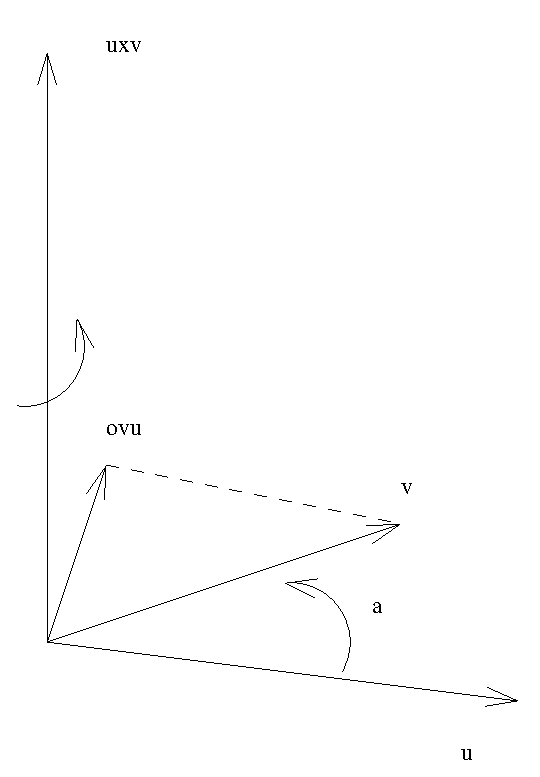
\includegraphics[height=1in]{../../modules/vectors/pictures/ok-cross_product.eps}
\end{figure}

\begin{itemize}
 \item If $\textbf{u}$, $\textbf{v}$ are non-zero and non-collinear vectors:\\
\begin{center}
 $\textbf{u} \times \textbf{v}$ is the vector determined by:
\end{center}
%
\begin{itemize}
 \item Support of direction of $\textbf{u} \times \textbf{v}$:
perpendicular to both $\textbf{u}$ and $\textbf{v}$;
 \item Direction of $\textbf{u} \times \textbf{v}$: given by Right Hand Rule;
 \item Magnitude of $\textbf{u} \times \textbf{v}$: product of $|\textbf{u}|$ and $|\textbf{orth}_{\bm{u}} \textbf{v}|$
%
$$|\textbf{u} \times \textbf{v}| = |\textbf{u}| \, |\textbf{orth}_u \textbf{v}| = |\textbf{u}| |\textbf{v}| \sin{\alpha}$$
%
\end{itemize}
\item If $\textbf{u}=\textbf{0}$ or $\textbf{v}=\textbf{0}$ or
$\textbf{u}$ and $\textbf{v}$ are collinear: \pause $\textbf{u} \times \textbf{v} = \textbf{0} $.
%
\end{itemize}

\end{frame}
\begin{frame}
 \frametitle{Properties of Cross Product}
Let $\textbf{u}$, $\textbf{v}$ non-zero vectors, $\alpha = \angle(\textbf{u},\textbf{v})$.


\begin{itemize}
\item<2-> $|\textbf{v} \times \textbf{u}|  = | \textbf{u} \times \textbf{v}|$.

\uncover<3->{Indeed, that is because $$|\textbf{orth}_{\bm{u}} \textbf{v}| = |\textbf{v}|\sin\alpha
\Longrightarrow |\textbf{u} \times \textbf{v}| = |\textbf{u}| \, |\textbf{v}| \, \sin{\alpha}$$
}

\item<4-> Cross product is anti-symmetric:
$$\textbf{v} \times \textbf{u} = - \textbf{u} \times \textbf{v} \; .$$
\item<5-> Cross product is linear in each argument:
%
$$ \textbf{u} \times (a\textbf{v} + b\textbf{w}) =
a \textbf{u} \times \textbf{v} + b \textbf{u} \times \textbf{w}$$
%
$$(a\textbf{u} + b\textbf{w}) \times \textbf{v} =
a \textbf{u} \times \textbf{v} + b \textbf{w} \times \textbf{v}$$
\end{itemize}

\end{frame}


\begin{frame}
\frametitle{$\fcv{orth}_{\fcv u}$ is a linear operator}
\begin{theorem}
$\alert<14>{ \alert<13>{ \fcv{orth}_{\fcv u}(\alert<12>{ \fcv v_1 +\fcv v_2}) }= \alert<10>{ \fcv{orth}_{\fcv u} \fcv v_1 } +\alert<11>{\fcv{orth}_{\fcv u} \fcv v_2}}$
\end{theorem}
\begin{proof}
\begin{columns}
\column{0.3\textwidth}
Geometric proof:
\uncover<8->{
\psset{xunit=0.9cm, yunit=0.9cm}
\begin{pspicture}(-0.5,-0.7)(3.8,4.2)%
\tiny%
\fcBoundingBox{-0.5}{-0.7}{3.8}{4.2}%
\uncover<9->{%
\fcParallelogramIIId{[0 -0.5 -0.5]}{[0 3 0]}{[0 0 3]}%
\fcPutIIId[lt]{[0.3 3 3]}{$\mathcal P$}%
}%
\fcLineIIId[arrows=->]{[0 0 0]}{[1 0 0]}%
\fcPutIIId[t]{[0.5 0 -0.1]}{$\fcv u$}%
\uncover<10->{%
\fcPerpendicularIIId{[1 1 2]}{[0 1 2]}{0.2}%
}%
\fcLineIIId[arrows=->]{[0 0 0]}{[1 1 2]}%
\fcPutIIId[tl]{[0.5 0.5 1]}{$\fcv v_1$}%
\uncover<10->{%
\fcLineIIId[linecolor=blue, arrows=->]{[0 0 0]}{[0 1 2]}%
\fcPutIIId[rb]{[0 0.5 1]}{$\color{blue}{\alert<14>{ \fcv{orth}_{\fcv u } \fcv v_1}}$}%
}%
\uncover<11->{\fcPerpendicularIIId{[1 2 0]}{[0 2 0]}{0.2}}%
\fcLineIIId[arrows=->]{[0 0 0]}{[1 2 0]}%
\fcPutIIId[t]{[0.5 1 -0.1]}{$\fcv v_2$}%
\uncover<11->{\fcLineIIId[linecolor=blue, arrows=->]{[0 0 0]}{[0 2 0]}}%
\uncover<11->{%
\fcLineIIId[arrows=->]{[1 1 2]}{[2 3 2]}%
\fcPutIIId[b]{[1.5 2 2]}{$\fcv v_2$}%
}%
\uncover<11->{%
\fcPerpendicularIIId{[2 3 2]}{[0 3 2]}{0.2}%
}%
\uncover<11->{%
\fcLineIIId[arrows=->, linecolor=blue]{[0 1 2]}{[0 3 2]}%
\fcPutIIId[b]{[0 2 2.2]}{$\color{blue}{\alert<14>{ \fcv{orth}_{\fcv u} \fcv v_2} }$}%
}%
\uncover<13->{%
\fcLineIIId[arrows=->, linecolor=blue]{[0 0 0]}{[0 3 2]}%
\fcPutIIId[l]{[0 2 1.3]}{$\color{blue}{\alert<14>{ \fcv{orth}_{\fcv u} (\fcv v_1 +\fcv v_2)}}$}%
}%
\uncover<12->{%
\fcLineIIId[arrows=->]{[0 0 0]}{[2 3 2]}%
\fcPutIIId[lt]{[1 1.5 1]}{$\fcv v_1 +\fcv v_2$}%
}%
\uncover<14>{%
\fcLineIIId[linewidth=1.5pt, arrows=->, linecolor=red]{[0 0 0]}{[0 3 2]}%
\fcLineIIId[linewidth=1.5pt, arrows=->, linecolor=red]{[0 1 2]}{[0 3 2]}%
\fcLineIIId[linewidth=1.5pt, arrows=->, linecolor=red]{[0 0 0]}{[0 1 2]}%
}%
\end{pspicture}
\uncover<9->{\alert<9>{Let $\mathcal P$: plane $\perp \fcv u$.}}
} %uncover
\column{0.7\textwidth}
Algebraic proof:

\small
\noindent \uncover<2->{
$
\begin{array}{r@{~}c@{~}l}
\fcv{orth}_{\fcv u}(\fcv v_1+\fcv v_2)&=& (\fcv v_1+\fcv v_2)- \alert<3>{\fcv{proj}_{\fcv u}(\fcv v_1 +\fcv v_2)}\\
\uncover<3->{&=&(\alert<4>{\fcv v_1}+\alert<5>{\fcv v_2})\alert<4,5>{-} \left(\alert<3>{ \alert<4>{\fcv{proj}_{\fcv u}(\fcv v_1)} +\alert<5>{\fcv{proj}_{\fcv u}(\fcv v_2)}}\right)} \\
\uncover<4->{&=&\left(\alert<4,6>{\fcv v_1- \fcv{proj}_{\fcv u}(\fcv v_1)}\right)+\left(\alert<5,7>{\fcv v_2-\fcv{proj}_{\fcv u}(\fcv v_2)}\right)}\\
\uncover<6->{&=& \alert<6>{\fcv{orth}_{\fcv u} \fcv v_1}+\alert<7>{\fcv{orth}_{\fcv u} \fcv v_2}}
\end{array}
$
}
\normalsize
\end{columns}
\end{proof}
\end{frame}
\begin{frame}
\frametitle{Geometric illustration of the linearity of $\times$ product}
\begin{theorem}
$\fcv u\times (\fcv v_1+\fcv v_2)=\fcv u \times\fcv v_1 +\fcv u\times \fcv v_2 $.
\end{theorem}
\psset{xunit=1.5cm, yunit=1.5cm}
\begin{pspicture}(-0.2, -1)(2,2)
\tiny
%\fcAxesIIId{2}{2}{2}
\fcLineIIId[arrows=->]{[0 0 0]}{[1 0 0]}%
\fcPutIIId[t]{[0.5 0 -0.1]}{$\fcv u$}%
\fcLineIIId[arrows=->]{[0 0 0]}{[1 1 0]}%
\fcPutIIId[t]{[0.5 0.5 0]}{$\fcv v_1$}%
\fcLineIIId[arrows=->]{[0 0 0]}{[1 2 1]}%
\fcPutIIId[tl]{[0.5 1 0.5]}{$\fcv v_2$}%
\fcLineIIId[arrows=->]{[1 1 0]}{[2 3 1]}%
\fcLineIIId[arrows=->]{[0 0 0]}{[2 3 1]}%
\fcPutIIId[lt]{[1 1.5 0.5]}{$\fcv v_1 +\fcv v_2$}%
\fcLineIIId[arrows=->]{[0 0 0]}{[0 0 1]}%
\fcPutIIId[l]{[0 0 0.5]}{$\fcv u\times \fcv v_1 $}%
\fcLineIIId[arrows=->]{[0 0 0]}{[0 -1 2]}%
\fcPutIIId[tr]{[0 -0.5 1]}{$\fcv u\times \fcv v_2 $}%
\fcLineIIId{[0 0 0]}{[0 -1 3]}
\fcPerpendicularIIId{[0 -1 2]}{[-1 0 0]}{0.3}%
\fcPerpendicularIIId{[0 -1 2]}{[-1 -2 -1]}{0.3}%
\fcPerpendicularIIId{[0 0 1]}{[-1 0 0]}{0.1}%
\fcPerpendicularIIId{[0 0 1]}{[-1 -1 0]}{0.1}%
\end{pspicture}
\end{frame}
\subsection{Determinants}
\begin{frame}
\frametitle{Permutations and permutation signs}
\begin{itemize}
\item Let $\sigma: \{1,2,\dots n\}\to \{1,2,\dots, n\}$ be one to one function.
\item<2-> Since $\sigma $ - one to one, $\left(\sigma(1), \sigma(2), \dots, \sigma(n) \right)$ have no repetition.
\uncover<3->{
\begin{definition}
A one-to-one function from the set $\{1,2,\dots, n\}$ to itself is called a \alert<4>{permutation} (``shuffling'').
\end{definition}
}
\item<4-> There are $n!$ different permutations: 
\begin{itemize}
\item<5-> there are $n$ ways to select $\sigma(1)$,
\item<6-> $n-1$ ways to select $\sigma(2)$ (one number is already taken),
\item<7-> and so on,  total: $n \cdot (n-1)\cdots 1 =n!$ ways to make a permutation.
\end{itemize}
\end{itemize}
\end{frame}
\begin{frame}
\frametitle{Sign of permutation}
\begin{itemize}
\item Given two sequences of numbers, define them to be transpositions of one another if one is obtained from the other with a \alert<1>{single swap of consecutive numbers}.
\item<2-> \alert<2>{$(2,\alert<3>{3,4},1) $ and $(2,\alert<3>{4,3},1) $ are} \uncover<3->{ \alert<3>{transpositions} of one another.}

\alert<4>{$(2,3,4,1) $ and $(1,3,4,2) $ are} \uncover<5->{\alert<5>{\textbf{not} transpositions} of one another.}
\item<6-> Write the numbers $\left(\sigma(1),\sigma(2), \dots, \sigma(n)\right)$ in a sequence. 
\item<7-> Using transpositions, get from $\left(\sigma(1),\sigma(2), \dots, \sigma(n)\right)$ to the properly ordered sequence $1,2,\dots, n$.
\item<8-> Number of transpositions used varies depending how we do it, but parity (even-ness) of \# of transpositions is always the same.
\item<10-> If $sign(\sigma)=1$,  $\sigma$ is called even, if $sign(\sigma)=-1$, $\sigma$ is called odd.
\end{itemize}
\uncover<9->{
\begin{definition}
If we can get from $\left(\sigma(1),\sigma(2), \dots, \sigma(n)\right)$ to $(1,2,\dots, n)$ with even \# of transpositions, define $sign(\sigma)$ to be $1$, else define $sign(\sigma)$ to be $-1$.
\end{definition}
}
\end{frame}
\begin{frame}
\begin{itemize}
\item To each permutation $\sigma$, assign $ n$ pairs of numbers $(1,\sigma(1))$, $(2, \sigma(2))$,\dots $(n,\sigma (n))$.
\item<2-> Consider a $n\times n$ chess board. \uncover<3->{Interpret pair $(k,\sigma(k))$ as $(row,column)$-coordinates in the board.} 
\item<4-> For each pair $(k,\sigma( k))$, place a rook on the board.
\item \uncover<5->{ Example: 
$
\begin{array}{rcl}
\alert<5,6>{\sigma(1)}  &\alert<5,6>{=}  & \alert<5,6>{2} \\
\alert<7,8>{\sigma(2)}  &\alert<7,8>{=}  & \alert<7,8>{3} \\
\alert<9,10>{\sigma(3)} &\alert<9,10>{=} & \alert<9,10>{4}\\
\alert<11,12>{\sigma(4)}&\alert<11,12>{=}& \alert<11,12>{1}
\end{array}
$, pairs:
$\begin{array}{rcl}
\alert<5,6>{(1,\sigma(1))}  &\alert<5,6>{=}  &\alert<5,6>{(1,2)} \\ 
\alert<7,8>{(2,\sigma(2))}  &\alert<7,8>{=}  &\alert<7,8>{(2,3)} \\ 
\alert<9,10>{(3,\sigma(3))} &\alert<9,10>{=} &\alert<9,10>{(3,4)} \\ 
\alert<11,12>{(4,\sigma(4))}&\alert<11,12>{=}&\alert<11,12>{(4,1)}
\end{array}
. $ 

Corresponding peaceful rook placement:
}

\uncover<2->{
\psset{xunit=2cm, yunit=2cm}
\begin{pspicture}(-0.2,0)(1,1.2)
\tiny
\fcBoundingBox{-0.2}{-0.1}{1}{1.2}
\psgrid[gridlabels=0, subgriddiv=4](0,0)(0,0)(1,1)
\uncover<3->{
\rput(-0.125, 0.875){$1$}
\rput(-0.125, 0.625){$2$}
\rput(-0.125, 0.375){$3$}
\rput(-0.125, 0.125){$4$}
\rput(0.125, 1.125){$1$}
\rput(0.375, 1.125){$2$}
\rput(0.625, 1.125){$3$}
\rput(0.875, 1.125){$4$}
}
\uncover<13>{
\psline[arrows=<->, linecolor=red](0,0.875)(1,0.875)
\psline[arrows=<-, linecolor=red](0.375,0)(0.375,0.875)
\psline[arrows=<->, linecolor=red](0,0.625)(1,0.625)
\psline[arrows=<->, linecolor=red](0.625,0)(0.625,1)
\psline[arrows=<-, linecolor=red](0,0.375)(0.875,0.375)
\psline[arrows=<->, linecolor=red](0.875,0)(0.875,1)
\psline[arrows=->, linecolor=red](0.125,0.125)(1,0.125)
\psline[arrows=->, linecolor=red](0.125,0.125)(0.125,1)
}
\uncover<5>{
\rput(0.125, 0.875){\alert<5>{\textbf{?}}}
\rput(0.375, 0.875){\alert<5>{\textbf{?}}}
\rput(0.625, 0.875){\alert<5>{\textbf{?}}}
\rput(0.875, 0.875){\alert<5>{\textbf{?}}}
}
\uncover<7>{
\rput(0.125, 0.625){\alert<7>{\textbf{?}}}
\rput(0.375, 0.625){\alert<7>{\textbf{?}}}
\rput(0.625, 0.625){\alert<7>{\textbf{?}}}
\rput(0.875, 0.625){\alert<7>{\textbf{?}}}
}
\uncover<9>{
\rput(0.125, 0.375){\alert<9>{\textbf{?}}}
\rput(0.375, 0.375){\alert<9>{\textbf{?}}}
\rput(0.625, 0.375){\alert<9>{\textbf{?}}}
\rput(0.875, 0.375){\alert<9>{\textbf{?}}}
}
\uncover<11>{
\rput(0.125, 0.125){\alert<11>{\textbf{?}}}
\rput(0.375, 0.125){\alert<11>{\textbf{?}}}
\rput(0.625, 0.125){\alert<11>{\textbf{?}}}
\rput(0.875, 0.125){\alert<11>{\textbf{?}}}
}
\uncover<6->{\fcFullDot{0.375}{0.875}}
\uncover<8->{\fcFullDot{0.625}{0.625}}
\uncover<10->{\fcFullDot{0.875}{0.375}}
\uncover<12->{\fcFullDot{0.125}{0.125}}
\end{pspicture}
}
\item<13-> Since $\sigma(k)$ are different, the rook placements are peaceful: rooks never hit one another. In other words, no two points lie on same column or row.
\end{itemize}

\vskip 10cm
\end{frame}

\begin{frame}
\frametitle{Square matrices}
\begin{itemize}
\item Let $A$ be $n\times n$ (square) table of numbers.
\item<2-> Technical term: $A$ is a (square) \emph{matrix}. 
\item<3-> Matrices are often denoted by surrounding with $\left(\right)$-parenthesis:
\[
A=\left(
\begin{array}{ccccc}
a_{\alert<7>{1}\alert<10>{1}} & a_{\alert<7>{1}\alert<11>{2}} & a_{\alert<7>{1}3}& \dots & a_{\alert<7>{1}\alert<12>{n}}\\
a_{\alert<8>{2}\alert<10>{1}} & a_{\alert<8>{2}\alert<11>{2}} & a_{\alert<8>{2}3}& \dots & a_{\alert<8>{2}\alert<12>{n}}\\
\vdots \\
a_{\alert<9>{n}\alert<10>{1}} & a_{\alert<9>{n}\alert<11>{2}} & a_{\alert<9>{n}3}& \dots & a_{\alert<9>{n}\alert<12>{n}}
\end{array}
\right).
\] 
\vphantom{ $n^{th}$ Second First row}
\only<7>{\alert<7>{First row}}
\only<8>{\alert<8>{Second row}}
\only<9>{\alert<9>{$n^{th}$ row}}
\only<10>{\alert<10>{First column}}
\only<11>{\alert<11>{Second column}}
\only<12>{\alert<12>{$n^{th}$ column}}

\item<4-> Most common convention for matrix notation: 
\begin{itemize}
\item $(i,j)^{th}$ entry of a matrix = denoted by letter with indices $i,j$, such as $a_{ij}$
\item<5-> no comma between indices $i,j$ in $a_{ij}$
\item<6-> first index stands for row, second - for column. 
\end{itemize}
\item<13-> Non-square matrices: used \& important but we discuss them elsewhere.
\end{itemize}
\end{frame}



\begin{frame}

\begin{itemize}
\item The determinant $\det A$ of a square matrix $A$ is a number written as:
\[
\det A= \left|\begin{array}{ccccc}
a_{11} & a_{12} & a_{13}& \dots & a_{1n}\\
a_{21} & a_{22} & a_{23}& \dots & a_{2n}\\
\vdots \\
a_{n1} & a_{n2} & a_{n3}& \dots & a_{nn}
\end{array} \right|
\]
\item<2-> The formula for the determinant is:

\[\det A=\sum_{\text{all permutations }\alert<3>{\sigma}} a_{\alert<4>{1\alert<3>{\sigma}(1)}} a_{\alert<4>{2\alert<3>{\sigma}(2)}} \dots a_{\alert<4>{n\alert<3>{\sigma}(n)}} \alert<6>{ sign(\alert<3>{\sigma})} \quad .
\]
\item<3-> For every permutation $\sigma$ we have one summand.
\item<4-> Every pair $(k,\sigma(k))$ can be identified with a placement of a rook placement (as described in previous slides/lectures).
\item<5-> For each rook placement we have a summand obtained by multiplying the numbers on which the rooks are standing.
\item<6-> The sign of each summand is determined by the sign of the permutation.
\end{itemize}

\vskip 10cm
\end{frame}

\begin{frame}

\frametitle{$2\times 2$ determinants}
\[
\det \left|
\begin{array}{cc}
\only<2,4>{\alert<2,4>{\bullet}}\only<1,3,5->{ a_{11}} & \only<1,2,4,6->{a_{12}}\only<3,5>{\alert<3,5>{\bullet}} \\
\only<1,2,4,6->{ a_{21}}\only<3,5>{\alert<3,5>{\bullet}} & \only<1,3,5->{ a_{22}}\only<2,4>{\alert<2,4>{\bullet}}
\end{array}
\right| = \uncover<4->{\alert<4>{ a_{11} a_{22}}} \uncover<6>{\alert<6>{-}}\uncover<5->{ \alert<5>{a_{12}a_{21}}}
\]
\begin{itemize}
\item We specialize the $n\times n$ determinant formula to the case $n=2$.
\item<2-> There are two peaceful rook placements for a $2\times 2$ chessboard.
\item<4-> For each peaceful rook placement we got one summand.
\item<6-> The permutation $(\sigma(1), \sigma(2))=(2,1)$ is odd, so one of the summands comes with negative sign.
\end{itemize}\end{frame}
\begin{frame}

\frametitle{$3\times 3$ determinants}
\[
\det \left|
\begin{array}{ccc}
\only<1-2,4-6,8->{ a_{11}}\only<3,7>{\alert<3,7>{\bullet}} & \only<1-3,5-7,9->{a_{12}}\only<4,8>{\alert<4,8>{\bullet}} &\only<1-4,7->{a_{13}}\only<5,6>{\alert<5,6>{\bullet}}\\
\only<1-4,6,7,9->{ a_{21}}\only<5,8>{\alert<5,8>{\bullet}} & \only<1-2,4-5,7->{ a_{22}}\only<3,6>{\alert<3,6>{\bullet}} & \only<1-3,5,6,8->{a_{23}}\only<4,7>{\alert<4,7>{\bullet}}\\
\only<1-3,5,7->{ a_{31}}\only<4,6>{\alert<4,6>{\bullet}} & \only<1-4,6,8->{ a_{32}}\only<5,7>{\alert<5,7>{\bullet}} & \only<1-2,4-7,9->{a_{33}}\only<3,8>{\alert<3,8>{\bullet}}
\end{array}
\right| =\begin{array}{l} \uncover<3->{\alert<3>{a_{11}a_{22}a_{33}}} \uncover<4->{\alert<4>{+}}
\uncover<4->{\alert<4>{a_{12}a_{23}a_{31}}} \\
\uncover<5->{\alert<5>{+}} \uncover<5->{\alert<5>{a_{13}a_{21}a_{32}}}\\
\uncover<6->{\alert<6>{-}} \uncover<6->{\alert<6>{a_{13}a_{22}a_{31}}} \uncover<7->{\alert<7>{-}} \uncover<7->{\alert<7>{a_{11}a_{23}a_{32}}} \\
\uncover<8->{\alert<8>{-}} \uncover<8->{\alert<8>{a_{12}a_{21}a_{33}}}
\end{array}
\]
\begin{itemize}
\item We specialize the $n\times n$ determinant formula to the case $n=3$.
\item<2-> There are $6=3!$ peaceful rook placements for a $3\times 3$ chessboard.
\item<3-> For each peaceful rook placement we got one summand.
\item<9-> The rook placements along the down-right ``broken'' diagonals correspond to even permutations, and the rook placements along the right-up ``broken'' diagonals correspond to negative permutations.
\end{itemize}\end{frame}
\subsection{Cross product in coordinates}
\begin{frame}
 \frametitle{Cross Product in Coordinates}

\begin{itemize}
 \item  $Oxyz$: rectangular coordinate system;
  \item $\textbf{i}$, $\textbf{j}$, $\textbf{k}$: unit vectors along fundamental directions.\pause
\end{itemize}
%
$$\textbf{i} \times \textbf{i} = \textbf{0} \quad , \quad \textbf{j} \times \textbf{j} =
\textbf{0} \quad , \quad \textbf{k} \times \textbf{k} = \textbf{0}$$
$$\textbf{i} \times \textbf{j} = \textbf{k} \quad , \quad \textbf{j} \times \textbf{k} =
\textbf{i} \quad , \quad \textbf{k} \times \textbf{i} = \textbf{j}$$
$$\textbf{j} \times \textbf{i} = -\textbf{k} \quad , \quad \textbf{k} \times \textbf{j} =
-\textbf{i} \quad , \quad \textbf{i} \times \textbf{k} = -\textbf{j}$$
\pause
If $\textbf{u} = u_1 \textbf{i} + u_2 \textbf{j} + u_3 \textbf{k} = \langle u_1, u_2, u_3 \rangle$,
 $\textbf{v}=v_1 \textbf{i} + v_2 \textbf{j} + v_3 \textbf{k} = \langle v_1, v_2, v_3 \rangle$:
%
$$\textbf{u} \times \textbf{v} = (u_1 \textbf{i} + u_2 \textbf{j} + u_3 \textbf{k})
\times (v_1 \textbf{i} + v_2 \textbf{j} + v_3 \textbf{k})= $$
%
$$= (u_2v_3 -u_3v_2) \textbf{i} + (u_3v_1-u_1v_3) \textbf{j} + (u_1v_2-u_2v_1) \textbf{k} \; .$$
\pause
$$\textbf{u} \times \textbf{v} = \langle u_1, u_2, u_3 \rangle \times \langle v_1, v_2, v_3 \rangle =
\left|  \begin{array}{ccc}
      \textbf{i} & \textbf{j} & \textbf{k} \\
      u_1 & u_2 & u_3 \\
      v_1 & v_2 & v_3
        \end{array}
\right|$$
\end{frame}
\begin{frame}
 \frametitle{Example}

$$\textbf{u} \times \textbf{v} = \langle u_1, u_2, u_3 \rangle \times \langle v_1, v_2, v_3 \rangle =
\left|  \begin{array}{ccc}
      \textbf{i} & \textbf{j} & \textbf{k} \\
      u_1 & u_2 & u_3 \\
      v_1 & v_2 & v_3
        \end{array}
\right|$$

If $\textbf{u} = \langle 1,2,3\rangle$ and $\textbf{v} = \langle 6,5,4 \rangle$, then
%
$$\textbf{u} \times \textbf{v} = \langle 1, 2, 3 \rangle \times \langle 6, 5, 4 \rangle =
\left|  \begin{array}{ccc}
      \textbf{i} & \textbf{j} & \textbf{k} \\
      1 & 2 & 3 \\
      6 & 5 & 4
        \end{array}
\right| = $$
%
$$= \left| \begin{array}{cc}
           2 & 3\\
	   5 & 4
          \end{array}
\right| \textbf{i} - \left| \begin{array}{cc}
           1 & 3\\
	   6 & 4
          \end{array}
\right| \textbf{j} + \left| \begin{array}{cc}
           1 & 2\\
	   6 & 5
          \end{array}
\right| \textbf{k}  = $$
%
$$=(2\cdot 4 -3\cdot 5) \textbf{i} - (1\cdot 4 - 3\cdot 6) \textbf{j} + (1 \cdot 5 - 2\cdot 6) \textbf{k} =$$
%
$$= -7 \textbf{i} + 14 \textbf{j} -7 \textbf{k} \; .$$
%
\end{frame}
\begin{frame}
\frametitle{Use $\times$ to find vector perpendicular to two given}
Recall $\textbf{u} \times \textbf{v}$ is perpendicular to $\textbf{u}$ and $\textbf{v}$.
\begin{example}
Find a vector perpendicular to $\textbf{u} =(1,1,0) = \textbf{i}+\textbf{j}$ and $\textbf{v}=\textbf{j}+\textbf{k}=( 0,1,1 )$:

\[
\begin{array}{rcl}
 \textbf{w} &= & (\textbf{i}+\textbf{j}) \times (\textbf{j}+\textbf{k}) =
\textbf{i} \times \textbf{j} + \textbf{i} \times \textbf{k} +
\textbf{j} \times \textbf{j} + \textbf{j} \times \textbf{k} = \\
& = & \textbf{k} -\textbf{j}+\textbf{0}+\textbf{i} = \textbf{i} - \textbf{j} + \textbf{k} = (1,-1,1)\; .
\end{array}
\]
\end{example}
\end{frame}

\begin{frame}
\frametitle{Use $\times$ to find area of triangle in space}
\begin{columns}
\column{0.3\textwidth}
\psset{xunit=2cm, yunit=2cm}
\begin{pspicture}(-0.3,-0.1)(1.4,1.4)%
\psline[arrows=->](0,0)(1.2,0)%
\psline[arrows=->](0,0)(0.2,1)%
\psline[arrows=->](1.2,0)(0.2,1)%
\psline(0.2,1)(1.4,1)(1.2,0)%
\rput[t](0,-0.1){$A$}
\rput[tl](1.2,-0.1){$B$}
\rput[bl](1.4,1.1){$D$}
\rput[br](0.2,1.1){$C$}
\uncover<2->{%
\rput[l](0.25,0.5){$\fcv w$}%
\fcPerpendicular{[0.2 1]}{[1 0]}{0.1}%
\psline[arrows=->](0.2,0 )(0.2,1)%
}%
\rput[t](0.5, -0.1){$\fcv u$}
\rput[r](0,0.5){$\fcv v$}
\end{pspicture}
\column{0.7\textwidth}
\begin{itemize}
\item $A$, $B$, $C$ points in space, $\textbf{u} = \textbf{AB}$, $\textbf{v}=\textbf{AC}$.
\item<2-> Then $|\textbf{w}| = |\textbf{orth}_{\bm{u}} \textbf{v}| = \text{ distance from } C \text{ to } AB\; .$
\item<3-> $|\textbf{u} \times \textbf{v}| = |\textbf{orth}_{\bm{u}} \textbf{v}| \, |\textbf{u}| =
2 \text{area}(ABC) = \text{area}(ABDC)$
\item<4-> $|\textbf{u} \times \textbf{v}|$ = Area of parallelogram on sides $\textbf{u}$ and $\textbf{v}$.
\end{itemize}
%
\end{columns}
\end{frame}

\begin{frame}
\begin{example}
\begin{columns}
\column{0.3\textwidth}
\psset{xunit=0.7cm, yunit=0.7cm}
\begin{pspicture}(-0.1, -1)(4,3.5)
\fcBoundingBox{-0.2}{-1}{4}{3.5}
\fcAxesIIId{3}{3}{3}%
\pscustom*[linecolor=cyan]{%
\fcPolyLineIIId{[1 2 3] [2 3 1] [3 1 2] [1 2 3]}
}
\end{pspicture}
\column{0.7\textwidth}

Find the area of the triangle $A(1,2,3)$, $B(2,3,1)$, $C(3,1,2)$.

\end{columns}
\[\begin{array}{rcl}
\displaystyle \text{Area}(ABC) &=&\displaystyle \frac{1}{2}|\textbf{AB} \times \textbf{AC}| =
\frac{1}{2}|( 1,1,-2) \times ( 2, -1, -1) | \\~\\
&=&\displaystyle\frac{1}{2} |( -3, -3, -3 )| \\~\\
&=&\displaystyle \frac{3\sqrt{3}}{2}\; .
\end{array}
\]

\end{example}
\end{frame}

\begin{frame}[label=current]
\frametitle{Scalar Triple Product}
\begin{columns}
\column{0.25\textwidth}
\begin{pspicture}(-0.4,-0.4)(2,2)%
\tiny%
\renewcommand{\fcScreenStyle}{z}%
\fcBoundingBox{-0.8}{-0.5}{3}{2}%
\uncover<2>{%
\fcLineIIId[linecolor=red, arrows=->]{[0 0 0]}{[0 2 0]}%
\fcLineIIId[linecolor=red, arrows=->]{[0 0 0]}{[1 0 0]}%
\fcLineIIId[linecolor=red, arrows=->]{[0 0 0]}{[0 1 1]}%
}%
\uncover<2->{%
\fcPutIIId[r]{[0.5 0 -0.1]}{$\fcv u $}%
\fcPutIIId[br]{[0 0.5 0.5]}{$\fcv w$}%
\fcPutIIId[br]{[0 1 0]}{$\fcv v$}%
}%
\uncover<4->{%
\fcPutIIId[r]{[0 0 1.3]}{$\fcv u \times \fcv v~~$}%
\fcLineIIId[arrows=->]{[0 0 0]}{[0 0 2]}%
\fcPerpendicularIIId[linestyle=dashed]{[0 1 1]}{[0 0 1]}{0.1}%
}%
\uncover<3->{\fcBoxIIId{[1 1 1]}{[1 0 0]}{[0 1 1]}{[1 3 1]}%
}%
\fcDotIIId{[0 0 0]}
\fcPutIIId[t]{[0 0 -0.1]}{$A$}
\fcDotIIId{[1 0 0]}
\fcPutIIId[t]{[1 0 -0.1]}{$B$}
\fcDotIIId{[0 1 1]}
\fcPutIIId[t]{[0 1 0.9]}{$D$}
\fcDotIIId{[0 2 0]}
\fcPutIIId[t]{[0 2 -0.1]}{$C$}
\end{pspicture}
\column{0.75\textwidth}
\begin{itemize}
\item $A$, $B$, $C$, $D$ points in space;
\item<2-> $\textbf{u} = \textbf{AB}$, $\textbf{v}=\textbf{AC}$, $\textbf{w}=\textbf{AD}$;
\item<3-> $R=R(\textbf{u},\textbf{v},\textbf{w})$: box on sides $\textbf{u}$, $\textbf{v}$, $\textbf{w}$.\pause
\item<4-> $\text{Vol}(R) = |\textbf{u} \times \textbf{v}| |\textbf{r}| = |\textbf{u} \times \textbf{v}| \, |\textbf{proj}_{\bm{u} \times \bm{v}} \textbf{w}| =
|\textbf{w} \cdot (\textbf{u} \times \textbf{v})|\; .$
\end{itemize}
\end{columns}
\uncover<5->{
\begin{definition}
The quantity $\textbf{w} \cdot (\textbf{u} \times \textbf{v})$ is called the scalar triple product of $\fcv w, \fcv u, \fcv v$.
\end{definition}
}
\uncover<6->{
\begin{itemize}
\item If $\textbf{u} =( u_1,u_2,u_3)$,
$\textbf{v} =( v_1,v_2,v_3)$, and $\textbf{w} =( w_1,w_2,w_3)$, then
%
$$\textbf{w} \cdot (\textbf{u} \times \textbf{v}) = \left|
\begin{array}{ccc}
w_1 & w_2 & w_3 \\
u_1 & u_2 & u_3 \\
v_1 & v_2 & v_3
\end{array}
 \right|$$
\end{itemize}
}
\end{frame}

\begin{frame}
  \frametitle{Orientations of Space}

\begin{itemize}
 \item The following are equivalent:
\begin{itemize}
  \item Every vector in space can be decomposed along $\textbf{u}$, $\textbf{v}$, $\textbf{w}$;
  \item The box $R(\textbf{u},\textbf{v},\textbf{w})$ is non-degenerate;
  \item $Vol(R(\textbf{u},\textbf{v},\textbf{w})) \neq 0$;
  \item $\textbf{u} \cdot (\textbf{v} \times \textbf{w}) \neq 0$.
\end{itemize}
%
\item \pause If any of the above is valid: $\{ \textbf{u}, \textbf{v}, \textbf{w}\}$ is a frame.

\item Rectangular coordinate system $\to$ fundamental frame $\{ \textbf{u}, \textbf{v}, \textbf{w}\}$

\item Consistent Right Hand Rule ($\textbf{w}=\textbf{u} \times \textbf{v}$) if and only if
%
$$\textbf{u} \cdot (\textbf{v} \times \textbf{w}) >0$$
%
The frame $\{ \textbf{u}, \textbf{v}, \textbf{w}\}$ is positively oriented if
$\textbf{u} \cdot (\textbf{v} \times \textbf{w}) >0$
%
\end{itemize}

\end{frame}
} %end lecture

% begin lecture
\lect{2014}{Lecture 4}{4}{

\begin{frame}
 \frametitle{Main Questions}


\begin{columns}[t]
\column[T]{0.4\textwidth}

\begin{pspicture}(-1,-2)(2,2)
\renewcommand{\fcScreen}{[-2 -1 -0.55] 0}
\tiny
\fcBoundingBox{-1}{-2}{2}{2}
\fcParallelogramIIId{[2 2 0]}{[1 2 -1]}{[1 2 2]}
\fcAxesIIId{2}{2}{2}
\fcLineIIId[arrows=->]{[ 0 0 0]}{[1 1 1]}
\fcDotIIId{[1 1 1]}
\fcPutIIId[lb]{[1 1 1]}{$~~Q(x,y,z)$}
\fcLineIIId{[0.6 0.95 0.35]}{[1.4 1.05 1.65]}

\fcLineIIId[arrows=->]{[ 0 0 0]}{[1 2 0.5]}
\fcDotIIId{[1 2 0.5]}
\fcPutIIId[lb]{[1 2 0.5]}{$~~P(x,y,z)$}
\end{pspicture}

\column{0.6\textwidth}
What condition(s) should
  \begin{itemize}
    \item the position vector
    \item the coordinates
  \end{itemize}

of a point satisfy for it to be on a specific

\begin{itemize}
    \item line $L$
    \item plane $\mathcal{P}$?
\end{itemize}
\end{columns}

Condition(s) in terms of:
\begin{itemize}
    \item position vector $\Rightarrow$ vectorial equations;
    \item coordinates $\Rightarrow$ scalar equations.
\end{itemize}
\end{frame}
\section{Equations of Lines}
\subsection{Line from point and direction}
\begin{frame}
\frametitle{Line from Point and Direction}
\begin{columns}
\column{0.3\textwidth}
\psset{xunit=1cm, yunit=1cm}
\begin{pspicture}(-0.2,-0.2)(3.5,2)
\tiny
\fcFullDot{0}{0}
\rput[tl](0,-0.1){$O$}
\psline(0, 1.7)(3.5,0.3)
\fcFullDot{0.5}{1.5}
\rput[bl](0.5, 1.5){$P_0$}
\uncover<4->{
\psline[arrows=->, linecolor=red](0.5,1.5)(2.5,0.7)
}
\psline[arrows=->, linecolor=blue](1,1.3)(2, 0.9)
\rput[b](1.5,1.2) {$\fcv u$}
\rput[l](3.5,0.3){$L$}

\uncover<2->{\psline[arrows=->](0,0)(0.5,1.5)
\rput[l](0.25, 0.75){$~~\fcv r_0$}
}
\uncover<3->{%
\psline[arrows=->](0,0)(2.5, 0.7)
\rput[b](2.5, 0.75){$P$}
\rput[t](1.25, 0.2){$\fcv r$}
}
\end{pspicture}

\column{0.7\textwidth}
\begin{itemize}
\item Suppose we have line $L$ that passes through point $P_0$ and has non-zero direction $\textbf{u}$.
\item<2-> Denote by $\fcv r_0=\fcv{OP}_0$ the position vector of $P_0$.
\item<3->$P$ with position vector $\textbf{r}$ is on $L$ $\Leftrightarrow$ 
\item<4->$\textbf{P}_0\textbf{P}$ has the same direction as $\textbf{u}$ $\Leftrightarrow$
\item<5-> $\textbf{P}_0\textbf{P}$ is a scalar multiple of $\textbf{u}$ $\Leftrightarrow$
\item<6-> $\textbf{r}-\textbf{r}_0 = t\textbf{u}$  for some real number $t$.
\end{itemize}
\end{columns}
\uncover<7->{
\begin{definition}
The equation 
\[
\fcv{r} = \fcv{r}_0+t\fcv{u}
\]
is called a parametric vectorial equation of the the line $L$.
\end{definition}
}
\end{frame}

\begin{frame}
\frametitle{Line from Point and Direction}
\begin{columns}
\column{0.3\textwidth}
\psset{xunit=1.4cm, yunit=1.4cm}
\begin{pspicture}(-0.2,-0.2)(2,2)
\renewcommand{\fcScreen}{[-3 -1 -0.2] 0}
\tiny
\fcAxesIIId{2}{2}{2}
\fcLineIIId{[0.5 0.5 1]}{[3 3 0.5]}
\fcLineIIId[arrows=->]{[0 0 0]}{[1 1 0.9]}
\fcPutIIId[tl]{[0.5 0.5 0.45]}{$~\fcv r_0$}

\fcLineIIId[linecolor=blue, arrows=->]{[1.5 1.5 0.8]}{[2 2 0.7]}
\fcPutIIId[bl]{[1.75 1.75 0.8]}{$\fcv u$}

\fcLineIIId[arrows=->]{[0 0 0]}{[2.5 2.5 0.6]}
\fcPutIIId[t]{[1.25 1.25 0.2]}{$\fcv r$}

\fcDotIIId{[1 1 0.9]}
\fcPutIIId[lb]{[1 1 0.95]}{$P_0$}
\fcDotIIId{[2.5 2.5 0.6]}
\fcPutIIId[lb]{[2.5 2.5 0.65]}{$P$}
\fcPutIIId[t]{[3 3 0.5]}{$~L$}
\end{pspicture}

$L$- line with direction $\textbf{u}$ passing through $P_0$

\column{0.7\textwidth}
\begin{itemize}
\item Point $P_0(x_0,y_0,z_0)$, $\fcv{r}_0=\langle x_0,y_0,z_0\rangle$;
\item Direction $\textbf{u}=\langle u_1,u_2,u_3\rangle$.
\uncover<2->{$P(x,y,z)$ with position vector $\textbf{r}$ is on $L$ $\Leftrightarrow$ \\ }
\uncover<3->{\medskip $\textbf{r} = \textbf{r}_0+t\textbf{u}$ $\Leftrightarrow$\\}
\uncover<4->{\medskip $\langle x,y,z\rangle = \langle x_0,y_0,z_0\rangle + t\langle u_1,u_2,u_3\rangle$ $\Leftrightarrow$\\}
\end{itemize}
\end{columns}
\begin{definition}
\uncover<5->{%
The equations 
\[
\left| \begin{array}{ll}
x & = x_0 + t u_1 \\
y & = y_0 + t u_2 \\
z & = z_0 + t u_3
\end{array}
\right., t\in \mathbb R
\]
are called \alert<5>{parametric scalar equations} of the line $L$.
}
\end{definition}

\end{frame}

\begin{frame}
\uncover<1->{%
\[
\left|
\begin{array}{ll}
x & = x_0 + t u_1 \\
y & = y_0 + t u_2 \\
z & = z_0 + t u_3
\end{array}
\right. \Longrightarrow \boxed{\frac{x-x_0}{u_1} = \frac{y-y_0}{u_2} = \frac{z-z_0}{u_3}} \text{ \textcolor[rgb]{0.98,0.00,0.00}{Symmetric equations}}\]
}%uncover
\begin{itemize}
\item<2->Caution! Symmetric equations are valid for $u_1,u_2,u_3\neq 0$. For example if $u_2=0$ the equations should be:
\[
\frac{x-x_0}{u_1} = \frac{z-z_0}{u_3} \quad  \text{ and } \quad y=y_0 
\]
\end{itemize}

\end{frame}
\begin{frame}
\begin{example}
$L$ - line with direction $\textbf{u} = ( 4,5,6)$ passing through $P_0(1,2,3)$. Find
\begin{itemize}
\item a parametric vectorial equation of $L$;
\item a parametric scalar equation of $L$;
\item symmetric equations of $L$.
\end{itemize}


\uncover<2->{%
Parametric vectorial equation:

$
\alert<2>{\fcv{r} =}\uncover<3->{\alert<3>{( 1,2,3) + t ( 4,5,6) \leftrightarrow \fcv{r} = ( 1+4t, 2+5t, 3+6t)}}
$
} %uncover

\uncover<3->{
Parametric scalar equations:

$
\left|
\begin{array}{rl}
\alert<4>{x =}& \uncover<5->{\alert<4>{ 1 + 4t}} \\
\alert<4>{y =}& \uncover<5->{\alert<4>{2+5t}} \\
\alert<4>{z =}& \uncover<5->{\alert<4>{3+6t}}
\end{array}
\right. , \quad t \text{ real number.}
$
} %uncover

\uncover<6->{ \alert<6>{Symmetric equations:}
\uncover<7->{

$
\displaystyle
\frac{x-1}{4} = \frac{y-2}{5} = \frac{z-3}{6}\; .
$
}
}
\end{example}
\end{frame}


\subsection{Line from two points}
\begin{frame}
 \frametitle{Line from Two Points}

\begin{columns}

\column{0.4\textwidth}
\psset{xunit=1.4cm, yunit=1.4cm}
\begin{pspicture}(-1,-0.4)(2.7,2.1)
\fcBoundingBox{-0.8}{-0.4}{4}{2.1}
\renewcommand{\fcScreen}{[-3 -1 -0.2] 0}
\tiny
\uncover<5->{\fcAxesIIId{2}{2}{2}}
\fcLineIIId{[0.5 0.5 1]}{[3 3 0.5]}
\fcLineIIId{[0.5 0.5 1]}{[4 4 0.3]}
\fcLineIIId[arrows=->]{[0 0 0]}{[1 1 0.9]}
\fcPutIIId[br]{[0.5 0.5 0.45]}{$\fcv r_0~$}

\fcLineIIId[linecolor=blue, arrows=->]{[1 1 0.9]}{[2.5 2.5 0.6]}
\fcPutIIId[br]{[1.75 1.75 0.8]}{$\fcv u$}

\fcLineIIId[arrows=->]{[0 0 0]}{[2.5 2.5 0.6]}
\fcPutIIId[b]{[1.25 1.25 0.3]}{$\fcv r_1$}

\fcDotIIId{[1 1 0.9]}
\fcPutIIId[lb]{[1 1 0.95]}{$P_0\uncover<5->{(x_0,y_0, z_0)} $}
\fcDotIIId{[2.5 2.5 0.6]}
\fcPutIIId[lb]{[2.5 2.5 0.65]}{$P_1\uncover<5->{(x_1, y_1, z_1)}$}
\fcDotIIId{[3.5 3.5 0.4]}
\fcLineIIId[arrows=->]{[0 0 0]}{[3.5 3.5 0.4]}
\fcPutIIId[b]{[1.75 1.75 0.2]}{$\fcv r$}
\fcPutIIId[b]{[3.5 3.5 0.5]}{$~P(x,y,z)$}
\fcPutIIId[t]{[4 4 0.3]}{$~L$}
\fcPutIIId[r]{[0 0 0.1]}{$O~~$}
\end{pspicture}
\column{0.6\textwidth}
\begin{itemize}
\item Given: distinct points $P_0$ and $P_1$, position vectors $\textbf{r}_0$ and $\textbf{r}_1$.
\item Goal: write equations of line $L$ through $P_0$ and $P_1$.
\item<2-> Direction of $L$: $\textbf{u} = \textbf{r}_1 - \textbf{r}_0$.
\item<5-> $\fcv{u} = ( x_1-x_0,y_1-y_0,z_1-z_0)$.
\end{itemize}
\end{columns}
\uncover<3->{
\begin{definition}
\alertNoH{1-}{Parametric equation} of a line $L$:\\
$
\textbf{r} = \textbf{r}_0 + t(\textbf{r}_1-\textbf{r}_0)
\quad \Leftrightarrow \quad   \textbf{r} = (1-t)\textbf{r}_0 + t\textbf{r}_1
$

\uncover<5->{
\alertNoH{1-}{Parametric scalar equations} of a line $L$:
$\left|
\begin{array}{ll}
x & = x_0 + t(x_1-x_0) \\
y & = y_0 + t(y_1-y_0) \\
z & = z_0 + t(z_1-z_0)
\end{array}
\right. \Leftrightarrow \left| \begin{array}{ll}
x & = (1-t)x_0 + tx_1 \\
y & = (1-t)y_0 + ty_1 \\
z & = (1-t)z_0 + tz_1
\end{array}
\right. , \quad t \text{ real number.}$
} %uncover
\end{definition}
} %uncover
\end{frame}

\begin{frame}
% \frametitle{Example}
\begin{example}

Write the equations of line $L$ through $P_0(1,2,3)$ and $P_1(5,2,1)$.

\begin{itemize}
\item<2-> Direction $\fcv u$ of $L$: \uncover<3->{$\fcv{u} = \fcv{r}_1-\fcv{r}_0 = \langle 4, 0, -2\rangle$.}
\item<4-> Parametric vectorial equation:

$  \uncover<4->{\alert<4,5>{\fcv{r}=}} \uncover<5->{
\alert<5>{ 
\langle 1,2,3\rangle + t \langle 4, 0 -2\rangle \Leftrightarrow  \fcv{r} = \langle 1+4t, 2, 3-2t\rangle
} .}
$
\item<6-> Parametric scalar equations:
\[\left|
\begin{array}{ll}
\alert<6,7>{x} & \alert<6,7>{=}\uncover<7->{\alert<7>{ 1+4t}} \\
\alert<6,7>{y} & \alert<6,7>{=}\uncover<7->{\alert<7>{ 2 }}\\
\alert<6,7>{z} & \alert<6,7>{=}\uncover<7->{\alert<7>{ 3-2t}}
\end{array}
\right. , \quad t \text{ real number.}\]
%
\item<8-> \alert<8>{Symmetric equations:}
\uncover<9->{
\[
\frac{x-1}{4} = \frac{z-3}{-2} \quad \text{ and } \quad y=2\; .\]
}
\end{itemize}
\end{example}
\end{frame}

\section{Equations of planes}
\subsection{Plane from point and normal}
\begin{frame}
\frametitle{Plane from Point and Normal}
\begin{columns}
\column{0.3\textwidth}
\psset{xunit=1cm, yunit=1cm}
\begin{pspicture}(-0.3, -1)( 3,3.3)
\tiny%
\renewcommand{\fcScreen}{[-1.5 2 -0.5 ] 0}%
\fcParallelogramIIId{[-0.1 -0.1 1]}{[1.6 -0.1 -0.7]}{[0 2 3]}%
\fcLineIIId[arrows=->]{[1 1 1]}{[2 0 2]}%
\fcPutIIId[l]{[1.5 0.5 1.5]}{$~~\fcv n\uncover<5->{( a,b,c)}$}%
\uncover<3->{%
\fcPerpendicularIIId{[2 0 2]}{ [1 1 1] [0.2 0.4 1.2]}{0.4}%
}%
\fcDotIIId{[1 1 1]}%
\fcPutIIId[lt]{[1 1 1]}{$P_0\uncover<6->{(x_0, y_0, z_0)}$}%
\uncover<2->{%
\fcDotIIId{[0.2 0.4 1.2]}%
\fcPutIIId[bl]{[0.2 0.4 1.2]}{$P\uncover<6->{(x,y,z)}$}%
}%
\uncover<3->{%
\fcLineIIId[arrows=->]{[1 1 1]}{[0.2 0.4 1.2]}%
}%
\fcLineIIId[arrows=->]{[0 0 0]}{[1 1 1]}%
\fcPutIIId[tl]{[0.5 0.5 0.5]}{$~\fcv r_0$}%
\uncover<2->{%
\fcLineIIId[arrows=->]{[0 0 0]}{[0.2 0.4 1.2]}%
}%
\fcPutIIId[r]{[0.1 0.2 0.6]}{$\fcv r~$}%
\fcAxesIIId{2}{2}{2}%
\end{pspicture}
\column{0.7\textwidth}
\begin{itemize}
\item<1-> Point $P_0$, with position vector $ \fcv{r}_0$;
\uncover<5->{$ \fcv{r}_0 = ( x_0,y_0,z_0)$}
\item<1-> Direction $ \fcv{n}$, non-zero vector.
\uncover<5->{$ \fcv{n} = ( a,b,c)$}
\item<1->Goal: describe plane passing through $P_0$ and orthogonal to $\fcv n$.
\item<2-> Point $P$ with position $ \fcv{r}$ is on $\mathcal{P}$ $\Leftrightarrow$
\item<3->{$ \alert<4>{\fcv{P}_0 \fcv{P}\uncover<4->{=\fcv r-\fcv r_0}} $ is orthogonal (normal) to $ \fcv{n}$ $\Leftrightarrow$}
\item<5->{\alert<5->{Implicit vectorial equation}: $ (\alert<8>{ \fcv{r}- \fcv{r}_0}) \cdot  \alert<9>{\fcv{n}} = 0.$}
\item<6->{A point $P(x,y,z)$ is on $\mathcal{P}$ $\Leftrightarrow$}

\end{itemize}
\end{columns}
\uncover<7->{%
\begin{definition}[\alert<7->{Implicit scalar equation}]
$\alert<8>{ ( x-x_0, y-y_0, z-z_0)} \cdot \alert<9>{( a,b,c)} = 0$ \uncover<10->{$\Leftrightarrow$}
\uncover<10->{\alert<10>{$a(x-x_0) + b(y-y_0)+c(z-z_0) = 0$}}
\end{definition}
} %uncover
\end{frame}

\begin{frame}
\begin{example}
Find the equation of the plane
\begin{itemize}
\item passing through $P_0(1,2,3)$ 
\item and perpendicular (normal) to the direction $ \fcv{n} = \langle 6,5,4\rangle$.
\end{itemize}
%
\uncover<2->{
$$6(x-1) + 5(y-2) + 4(z-3) = 0$$

$$6x +5y+4z = 28$$
}

\end{example}
\pause The general equation of a plane is given by:
%
$$ax+by+cz = d .$$
%
The coefficients $a,b,c$ are \pause the components of normal to the plane,
%
$$ \fcv{n} = \langle a,b,c\rangle\; .$$

\end{frame}

\subsection{Plane from two directions}
\begin{frame}
 \frametitle{Plane from Point and two Directions}

\begin{columns}
\column{0.45\textwidth}
\begin{pspicture}(-1.9,-1.7)(2,2.2)%
\tiny%
\renewcommand{\fcScreen}{[-4 -1 -0.4] 0}%
\fcBoundingBox{-1.9}{-1.7}{2}{2.2}%
\uncover<3->{%
\fcParallelogramIIId{[0.1 -1.9 1.36]}{[3.1 1.1 0.16]}{[-3.2 0.8 1.48]}%
}%
\fcAxesIIId{2}{2}{2}
%normal: (0.2 0.2 1)
\uncover<2->{%
\fcLineIIId[arrows=->, linecolor=blue]{[1 3 -1]}{ [1.6 3.6 -1.24]}
\fcPutIIId[rt]{[1.3 3.3 -1.12]}{$\fcv u$}
\fcLineIIId[arrows=->, linecolor=brown]{[1 3 -1]}{[0.45 3.45 -0.98]}
\fcPutIIId[b]{[0.725 3.225 -0.99]}{$\fcv v ~$}
}%
\uncover<4->{%
\fcLineIIId[arrows=->, linecolor=red]{[1 3 -1]}{[1.24 3.24 0.2]}
\fcPutIIId[l]{[1.12 3.12 -0.4]}{$\fcv u \times \fcv v $}%
}%
\uncover<3->{%
\fcLineIIId[linewidth=0.3pt, linecolor=gray]{[0.43 -0.17 0.948]}{[-1.55 1.45 1.02]}%
\fcLineIIId[linewidth=0.3pt, linecolor=gray]{[-0.2 -0.2 1.08]}{[1.6 1.6 0.36]}%
}%
\uncover<4->{\fcLineIIId[arrows=->, linecolor=red]{[0.1 0.1 0.96]}{[0.34 0.34 2.16]}}
\uncover<9->{%vectors su, tv
\fcLineIIId[arrows=->]{[0.1 0.1 0.96]}{[1.3 1.3 0.48]}
\fcPutIIId[tr]{[1.2 1.2 0.5]}{$s\fcv u~~$}
\fcLineIIId[arrows=->]{[0.1 0.1 0.96]}{[-1 1 1]}
\fcPutIIId[b]{[-0.8 0.9 1.1]}{$t\fcv v$}
}%
\uncover<2->{%the vectors u,v
\fcLineIIId[arrows=->, linecolor=blue]{[0.1 0.1 0.96]}{[0.7 0.7 0.72]}%
\fcPutIIId[rt]{[0.4 0.4 0.84]}{$\fcv u$}%
\fcLineIIId[arrows=->, linecolor=brown]{[0.1 0.1 0.96]}{[-0.45 0.55 0.98]}%
\fcPutIIId[b]{[-0.175 0.325 0.97]}{$\fcv v$}%
}%uncover
\uncover<9->{%lines making the parallelogram
\fcLineIIId{[-1 1 1]}{ [0.2 2.2 0.52]}%
\fcLineIIId{[1.3 1.3 0.48]}{[0.2 2.2 0.52]}%
}%
\uncover<8->{%vector P_0P
\fcLineIIId[arrows=->]{[0.1 0.1 0.96]}{[0.2 2.2 0.52]}%
}%
\fcLineIIId[arrows=->]{[0 0 0]}{[0.1 0.1 0.96]}
\fcPutIIId[l]{[0.05 0.05 0.48]}{$~\fcv r_0$}

\uncover<7->{%
\fcLineIIId[arrows=->]{[0 0 0]}{[0.2 2.2 0.52]}
\fcPutIIId[tl]{[0.1 1.1 0.26]}{$~\fcv r$}
\fcDotIIId{[0.2 2.2 0.52]}
\fcPutIIId[tl]{[0.2 2.2 0.52]}{$P$}
}%
\fcDotIIId{[0.1 0.1 0.96]}
\fcPutIIId[br]{[0.1 0.1 0.96]}{$P_0~~$}
\end{pspicture}
\column{0.55\textwidth}
\begin{itemize}
\item Given: point $P_0$ with position vector $\fcv{r}_0$. \item<2-> Non-parallel directions $\fcv{u}$ and $\fcv{v}$.
\item<3-> Goal: give equations of plane $\mathcal P$ through $P_0$ and parallel to both $\fcv{u}$ and $\fcv{v}$.
\end{itemize}
\end{columns}
\only<4-6>{%
\uncover<4->{Normal direction $\fcv{n} = \fcv{u} \times \fcv{v} \neq \fcv{0}$. }

\uncover<5->{\alert<1->{Implicit equation}: $P(\fcv{r}) \text{ is on } \mathcal{P} \Longleftrightarrow (\fcv{r}-\fcv{r}_0) \cdot \fcv{n} = 0$}
\uncover<6->{Interpretation:$$\text{Vol}(R(\fcv{r} - \fcv{r}_0,\fcv{u},\fcv{v})) = 0$$}
} %uncover

\only<7-10>{$P(\fcv{r})$ is on the plane $\mathcal{P}$ $\Leftrightarrow$

\uncover<8->{ $\fcv{P}_0\fcv{P}$ is a combination of $\fcv{u}$, $\fcv{v}$ $\Leftrightarrow$
}

\uncover<9->{There are scalars $s$, $t$ such that $\fcv{r}-\fcv{r}_0= s\fcv{u} + t\fcv{v} \Leftrightarrow $}

\uncover<10->{%
\alert<1->{Parametric equation}:
\[\alert<10>{ \fcv{r} = \fcv{r}_0 + s\fcv{u} + t\fcv{v}}
\]
for some parameters $s$ and $t$.
}%uncover
}%only<7-?>
\only<11->{
\alert<1->{Parametric equation}:
\[
\alert<11>{ \alert<13>{\fcv{r}} = \alert<14>{\fcv{r}_0} + s \alert<15>{\fcv{u}} + t\alert<16>{\fcv{v}}}
\]

\uncover<12->{Let $P_0(x_0,y_0,z_0)$, $P(x,y,z)$ $\fcv{u} = \langle u_1,u_2,u_3\rangle$, $\fcv{v}=\langle v_1,v_2,v_3\rangle$.} \uncover<13->{$\Rightarrow$}

\uncover<13->{
\alert<1->{Parametric scalar equations}:
$$\left|\begin{array}{ll}
\alert<13>{x} = & \alert<14>{x_0} + s\alert<15>{u_1}+t\alert<16>{v_1} \\
\alert<13>{y} = & \alert<14>{y_0} + s\alert<15>{u_2}+t\alert<16>{v_2} \\
\alert<13>{z} = & \alert<14>{z_0} + s\alert<15>{u_3}+t\alert<16>{v_3}
\end{array}
\right., \text{for } s, t \text{ real parameters}.
$$
}
}
\vskip 10cm
\end{frame}




\begin{frame}
 \frametitle{Example}

$P_0(1,2,3)$, $\textbf{u}=\langle -1,0,2\rangle$, $\textbf{v} = \langle 0,-2,1\rangle$.\pause
%
$$\textbf{n} = \textbf{u} \times \textbf{v} = \left| \begin{array}{ccc}
                           \textbf{i} & \textbf{j} & \textbf{k} \\
			   -1 & 0 & 2 \\
                           0 & -2 & 1
                          \end{array}
\right| = 4\textbf{i}+\textbf{j} +2\textbf{k}$$
%
$$4(x-1)+1(y-2) + 2(z-3) = 0 \Longleftrightarrow 4x+y+2z = 12$$
%
\pause Implicit scalar equation:
%
$$4x+y+2z = 12\; .$$

\pause Parametric vectorial equation:
%
$$\langle x, y, z \rangle = \langle 1,2,3\rangle + s\langle -1, 0, 2\rangle + t\langle 0,-2,1\rangle$$

\pause Parametric scalar equations:
%
$$\left\{ \begin{array}{ll}
           x & = 1 -s \\
           y & = 2-2t \\
           z & = 3 +2s +t
          \end{array}
\right. \quad s,t \text{ real parameters}.$$
%
\end{frame}

\subsection{Plane from three points}
\begin{frame}
 \frametitle{Plane from Three Points}

\begin{columns}
\column{0.4\textwidth}
\psset{xunit=0.8cm, yunit=0.8cm}
\begin{pspicture}(-2.2, -2.2)(3,3)
\tiny
\renewcommand{\fcScreen}{[-2 -1 -0.5] 0}
\fcParallelogramIIId{[-0.8 -0.8 3.6]}{[-1.4 2.4 1]}{[2.4 -1.4 1]}
\fcPutIIId[l]{[0 0 0.05]}{$~~O$}
\fcDotIIId{[0 0 0]}

\fcLineIIId[arrows=->, linestyle=dotted]{[0 0 0]}{[2 0 0]}
%\fcPutIIId{[1 0 0]}{$\fcv r_2$}
\fcLineIIId[arrows=->, linestyle=dotted]{[0 0 0]}{[0 2 0]}
%\fcPutIIId{[0 1 0]}{$\fcv r_0$}
\fcLineIIId[arrows=->, linestyle=dotted]{[0 0 0]}{[0 -0.4 2.4]}
%\fcPutIIId{[0 -0.2 1.2]}{$\fcv r_1$}
\fcDotIIId{[2 0 0]}
\fcDotIIId{[0 2 0]}
\fcDotIIId{[0 -0.4 2.4]}
\fcPutIIId[r]{[2 0 0]}{ $P_2(\fcv r_2)~$}
\fcPutIIId[tl]{[0 2 0]}{ $P_0(\fcv r_0)$}
\fcPutIIId[b]{[0 -0.4 2.4]}{ $P_1(\fcv r_1)$}
\fcLineIIId[arrows=->]{[0 2 0]}{[2 0 0]}
\fcPutIIId[t]{[1 1 -0.1]}{$~\fcv v$}
\fcLineIIId[arrows=->]{[0 2 0]}{[0 -0.4 2.4]}
\fcPutIIId[b]{[0 0.8 1.3]}{$~\fcv u$}%
\fcPerpendicularIIId{[4.8 6.8 4.8]}{ [0 2 0] [2 0 0]}{0.6}%
\fcPerpendicularIIId[arrows=<-]{[4.8 6.8 4.8]}{[0 2 0] [0 -0.4 2.4]}{0.6}%
\fcLineIIId[linestyle=dotted]{[0 0 0]}{[1.4 -0.84 1.44]}%
\fcPerpendicularIIId[arrows=<-]{[4.8 6.8 4.8]}{[0 2 0] [1.4 -0.84 1.44]}{0.8}%
\fcLineIIId[arrows=->]{[0 2 0]}{[1.4 -0.84 1.44]}%
\fcPutIIId[b]{[1.4 -0.84 1.44]}{$P(\fcv r)$}%
\end{pspicture}

\column{0.6\textwidth}
\begin{itemize}
\item Given: three non-collinear points $P_0(\fcv{r}_0)$, $P_1(\fcv{r}_1)$, $P_2(\fcv{r}_2)$.
\item Goal: find equations fo plane $\mathcal{P}$ passing through $P_0$, $P_1$, and $P_2$.
\item<2-> The plane is parallel to $\fcv{u} = \fcv{P}_0\fcv{P}_1 = \fcv{r}_1 -\fcv{r}_0$ and passing through $P_0$ $\Rightarrow$ this problem was solved previously.

\end{itemize}
\end{columns}
\only<3>{
Normal $\fcv{n} = \fcv{u} \times \fcv{v} =
(\fcv{r}_1-\fcv{r}_0) \times (\fcv{r}_2-\fcv{r}_0)$  \\

\alert<1->{Implicit equation}:
$$(\fcv{r}-\fcv{r}_0) \cdot \fcv{n} = 0$$
$$\boxed{(\fcv{r}-\fcv{r}_0) \cdot [(\fcv{r}_1-\fcv{r}_0) \times (\fcv{r}_2-\fcv{r}_0)] = 0}$$
$$\text{Vol}(R(\fcv{P}_0\fcv{P}, \fcv{P}_0\fcv{P}_1, \fcv{P}_0\fcv{P}_2)) = 0$$
}

\only<4>{
\alert<1->{Implicit equation}: $(\fcv{r}-\fcv{r}_0) \cdot [(\fcv{r}_1-\fcv{r}_0) \times (\fcv{r}_2-\fcv{r}_0)] = 0$

Let the points have coordinates $P_0(x_0,y_0,z_0)$, $P_1(x_1,y_1,z_1)$, $P_2(x_2,y_2,z_2)$. $P(x,y,z)$ is on plane $\mathcal{P}$:

\alert<1->{Implicit scalar equation}:
$\left| \begin{array}{ccc}
x-x_0 & y-y_0 & z-z_0 \\
x_1-x_0 & y_1-y_0 & z_1-z_0 \\
x_2-x_0 & y_2-y_0 & z_2-z_0
\end{array}
\right| = 0\; .$
}

\vskip 10cm
\end{frame}


\begin{frame}
\begin{example}
Let $P_0(a,0,0)$, $P_1(0,b,0)$  $P_2(0,0,c)$ be three points, $a,b,c\neq 0$. Find plane $\mathcal{P}$ passing through $P_0$, $P_1$, $P_2$ (i.e., plane with prescribed $x,y,z$-intercepts).

\bigskip

\begin{columns}
\column{0.3\textwidth}
\psset{xunit=1cm, yunit=1cm}
\begin{pspicture}(-1.3,-0.6)(2.5,2.2)
\tiny
\renewcommand{\fcScreen}{[-5 -1 -0.5] 0}
\fcBoundingBox{-1.3}{-0.6}{2.5}{2.2}
\pscustom*[linecolor=cyan]{%
\fcLineIIId{[1 0 0]}{[0 1.2 0]}%
\fcLineIIId{[0 1.2 0]}{[0 0 1]}%
\fcLineIIId{[0 0 1]}{[1 0 0]}%
}%
\fcLineIIId[linestyle=dotted]{[0 0 0]}{[1 0 0]}%
\fcLineIIId[linestyle=dotted]{[0 0 0]}{[0 1.2 0]}%
\fcLineIIId[linestyle=dotted]{[0 0 0]}{[0 0 1]}%
\fcLineIIId[arrows=->]{[0 0 1]}{[0 0 2]}%
\fcLineIIId[arrows=->]{[0 1.2 0]}{[0 2 0]}%
\fcLineIIId[arrows=->]{[1 0 0]}{[4 0 0]}%
\fcPutIIId[t]{[4 0 0]}{$x$}%
\fcPutIIId[t]{[0 2 0]}{$y$}%
\fcPutIIId[b]{[0 0 2]}{$z$}%
\fcLineIIId[arrows=->]{[1 0 0]}{[0 1.2 0]}%
\fcPutIIId[t]{[0.5 0.6 -0.1]}{$\fcv u$} %
\fcLineIIId[arrows=->]{[1 0 0]}{[0 0 1]}%
\fcPutIIId[r]{[0.5 0 0.5]}{$\fcv v~$} %
\fcLineIIId{[0 1.2 0]}{[0 0 1]}%
\fcLineIIId[arrows=->]{[1 0 0]}{[2.2 1 1.2]}%
\fcPutIIId[l]{[1.6 0.5 0.6]}{$~~\fcv n$} %
\fcPerpendicularIIId{[2.2 1 1.2]}{[1 0 0] [0 0 1]}{0.2}%
\fcPerpendicularIIId{[2.2 1 1.2]}{[1 0 0] [0 1.2 0]}{0.2}%
\fcDotIIId{[1 0 0]}
\fcPutIIId[rb]{[1 0 0]}{$P_0(a, 0,0)$}
\fcDotIIId{[0 1.2 0]}
\fcPutIIId[lb]{[0 1.2 0]}{$~P_1 (0, b, 0)$}
\fcDotIIId{[0 0 1]}
\fcPutIIId[l]{[0 0 1.2]}{$~P_2(0,0,c)$ }
\end{pspicture}

\column{0.7\textwidth}
\uncover<2->{\alertNoH{2,3}{$\mathcal{P}$: parallel to}} \uncover<3->{\alertNoH{3}{%
$\textbf{P}_0\textbf{P}_1 = ( -a, b, 0), \textbf{P}_0\textbf{P}_2 = ( -a, 0, c).$
}} %alert, uncover

\uncover<4->{\alertNoH{4,5}{Normal:} }
\uncover<5->{\alertNoH{5}{%
$$\textbf{n} =\textbf{P}_0\textbf{P}_1 \times \textbf{P}_0\textbf{P}_2=
\left| \begin{array}{ccc}
\textbf{i} & \textbf{j} & \textbf{k} \\
-a & b & 0 \\
-a & 0 & c
\end{array}
\right| = bc \textbf{i} + ac \textbf{j} + ab \textbf{k}.$$
}}%alert, uncover

\uncover<6->{\alertNoH{6}{Implicit scalar equation of plane:}}

\[
\begin{array}{rcl}
\uncover<7->{( x-a, y, z ) \cdot ( bc, ac, ab ) &=& 0}\\
\uncover<8->{bcx+acy + abz &=& abc} \\
\displaystyle \uncover<9->{\frac{x}{a} + \frac{y}{b} + \frac{z}{c} &=& 1}
\end{array}
\]

\end{columns}
\end{example}
\end{frame}


\section{Distances, Angles, Parallelism, Incidence}
\begin{frame}
\frametitle{Relationships betwee points lines and planes}

\begin{itemize}
\item So far we studied the following geometric objects/
\begin{itemize}
\item Points: $P(\textbf{r})$.
\item Lines: $L$: $\textbf{r}= \textbf{r}_0 + t\textbf{u}$
\item Planes: $\mathcal{P}$: $(\textbf{r}-\textbf{r}_0)\cdot \textbf{n} =0$
\end{itemize}
\item We investigate the following relationships/geometric quantities:
\begin{itemize}
\item Parallelism
\item Perpendicularity
\item Angles
\item Distances
\item Intersections
\end{itemize}
\end{itemize}
\end{frame}
\subsection{Distance Between Point and Line}
\begin{frame}
\frametitle{Point and line}

\begin{columns}
\column{0.4\textwidth}
\psset{xunit=1cm, yunit=1cm}
\begin{pspicture}(-0.6, -0.5)(3.8,2.2)%
\tiny%
\fcBoundingBox{-0.2}{-0.5}{3.2}{2.2}%
\psline[linecolor=gray](-0.3, -0.1)(3, 1)%
\fcFullDot{0}{0}
\fcFullDot{2}{2}
\rput[lt](3,1){$L$}%
\psline[arrows=->, linecolor=red](0,0)(0.9, 0.3)%
\rput[tl](0.45, 0.05){$~\fcv u$}%
\psline[arrows=->, linecolor=green](0,0)(2,2)%
\rput[r](1,1){$\fcv r_1-\fcv r_0$}%
\rput[b](2,2){$P(\fcv r_1)$}%
\fcPerpendicular[arrows=<-, linecolor=blue]{[2 2]}{[3 1]}{0.2}%
\rput[l](2.25, 1.5){$\fcv{orth}_{\fcv u}(\fcv r_1-\fcv r_0)$}
\rput[t](0,-0.1){$P_0(\fcv r_0)$}
\end{pspicture}
\column{0.6\textwidth}
\begin{itemize}
\item Given: Point $P(\fcv{r}_1)$,
\item line $L: \quad \fcv{r}=\fcv{r}_0+t\fcv{u}$.
\item Goal: find the distance between $P$ and $L$.
\end{itemize}
\end{columns}

\alertNoH{1-}{Distance} from $P$ to $L$:

\uncover<2->{
\[\begin{array}{rcll|l}
d(P,L) &=&\displaystyle \left|\fcv{orth}_{\fcv{u}}(\fcv{r}_1-\fcv{r}_0)\right|\\~\\
\uncover<3->{%
d(P,L) &=&\displaystyle \left|\fcv r_1- \fcv r_0- \frac{(\fcv{r}_1-\fcv{r}_0)\cdot \fcv u}{ \fcv u \cdot \fcv u} \fcv u \right|\\~\\
}%uncover
\uncover<4->{%
d(P,L) &=&\displaystyle \frac{|(\fcv{r}_1-\fcv{r}_0) \times \fcv{u}|}{|\fcv{u}|} &&\text{Valid only in } 3 \text{ dimensions!}
}%uncover
\end{array}
\]
}

\end{frame}

\begin{frame}
\frametitle{Distance between point and plane}
\begin{columns}
\column{0.4\textwidth}
\begin{pspicture}(-0.2,-0.2)(2,2)
\tiny
\fcParallelogramIIId{[-1 -1 0]}{[2 -1 0]}{[-1 2 0]}

\fcPutIIId[t]{[2 0.5 0]}{$\mathcal P$}
\fcPutIIId[t]{[0 0 -0.05]}{$P_0(\fcv r_0)$}
\fcPutIIId[bl]{[1 1 2]}{$~P(\fcv r_1)$}

\fcLineIIId[linestyle=dotted]{[0 0 -0.2]}{[0 0 2.2]}
\fcPerpendicularIIId[linestyle=dotted]{[1 1 2]}{[0 0 1]}{0.2}
\fcLineIIId[arrows=->, linecolor=red]{[0 0 0]}{[0 0 1]}
\fcPutIIId[r]{[0 0 0.5]}{$\fcv n~~$}


\fcLineIIId[arrows=->, linecolor=green]{[0 0 0]}{[1 1 2]}
\fcPutIIId[rb]{[0.7 0.7 1.4]}{$\fcv r_1-\fcv r_0$}


\fcPerpendicularIIId[arrows=<-, linecolor=blue]{[1 1 2]}{[1 1 0]}{0.2}
\fcPutIIId[l]{[1 1 1]}{$~\fcv{proj}_{\fcv n} (\fcv r_1-\fcv r_0)$}

\fcLineIIId[linecolor=gray]{[-0.7 -0.7 0]}{[1.7 1.7 0]}
\fcDotIIId{[1 1 2]}
\fcPutIIId[bl]{$P(\fcv r_1)$}

\end{pspicture}
\column{0.6\textwidth}
\begin{itemize}
\item Given: point $P(\fcv{r}_1)=(x_1, y_1, z_1)$,
\item plane $\mathcal{P}: \quad (\fcv{r}-\fcv{r}_0)\cdot \fcv{n} = 0$.
\item Goal: find the distance between $P$ and $\mathcal P$. 
\end{itemize}
\end{columns}
\alert<1->{Distance} from $P$ to $\mathcal{P}$:
\uncover<2->{
$$\begin{array}{rcl}
d(P,\mathcal{P}) &\alert<0>{=}&\displaystyle |\fcv{\text{proj}}_{\fcv{n}}( \fcv{r}_1-\fcv{r}_0)|\\
\alert<7>{d(P,\mathcal{P})} &\alert<7>{=}&\displaystyle \alert<7>{ \frac{|(\fcv{r}_1- \fcv{r }_0) \cdot \fcv{n}|}{|\fcv{n}|}}
\end{array}
$$
}

\uncover<3->{\alert<1->{Scalar equation}: 
$P(x_1,y_1,z_1)$
$
\begin{array}{rrcl}
\mathcal{P}:& \alert<4>{a} \alert<5>{x}+ \alert<4>{b}\alert<5>{y}+ \alert<4>{c} \alert<5>{z} +\alert<6,9>{ d} = (\alert<5>{\fcv r} \alert<6,9>{- \fcv r_0})\alert<6,9>{\cdot\alert<4>{\fcv n}}&=&0\\
\uncover<4->{
&\alert<4>{\fcv{n}} &=& \alert<4>{\langle a,b,c\rangle} }\\
\uncover<7->{&\displaystyle \alert<7>{ d(P, \mathcal P)= \frac{|( \alert<8>{ \fcv{r}_1} \alert<9>{-\fcv{r}_0}) \alert<8,9>{\cdot \fcv{n}}|}{\alert<10>{|\fcv{n}|}}} & =&\displaystyle \frac{|\alert<8>{ax_1+by_1+cz_1} +\alert<9>{d} |}{\alert<10>{ \sqrt{a^2+b^2+c^2}}}}
\end{array}$
}
\end{frame}

\subsection{Parallel Lines}
\begin{frame}
  \frametitle{Parallel lines}
    Lines
    $$L_1: \quad \textbf{r}= \textbf{r}_1+t\textbf{u}_1 \qquad L_2: \quad \textbf{r}= \textbf{r}_2+s\textbf{u}_2$$
\begin{columns}[t]
  \column[T]{6cm}
  \textcolor[rgb]{0.98,0.00,0.00}{Parallel} lines\\
    %\medskip
    \uncover<2->{
    $L_1 || L_2$ $\Longleftrightarrow$
    $\textbf{u}_1$, $\textbf{u}_2$ collinear $\Longleftrightarrow$
    $$\boxed{\textbf{u}_1 \times \textbf{u}_2 = \textbf{0}}$$}
    \uncover<3->{
    \textcolor[rgb]{0.98,0.00,0.00}{Distance}:
    $$d= d(L_1,L_2)  = d(P_1,L_2) = d(P_2,L_1)$$}
    \uncover<4->{
    $$d= d(L_1,L_2) = |\textbf{\text{orth}}_{\bm{u}_1} (\textbf{r}_2-\textbf{r}_1)|$$
    $$\boxed{d = \frac{|(\textbf{r}_2-\textbf{r}_1) \times \textbf{u}_1|}{|\textbf{u}_1|} =\frac{|(\textbf{r}_2-\textbf{r}_1) \times \textbf{u}_2|}{|\textbf{u}_2|}}$$}
    %\textcolor[rgb]{0.98,0.00,0.00}{Identical} lines: $d(L_1,L_2)=0$
    %$$\textbf{u}_1\times \textbf{u}_2 = \textbf{0} \text{ and }
    %(\textbf{r}_2-\textbf{r}_1) \times \textbf{u}_1 = \textbf{0}$$
  \column{6.5cm}
  \begin{figure}
        \psfrag{L1}{$L_1$}
        \psfrag{L2}{$L_2$}
        \psfrag{P1}{$P_1$}
        \psfrag{P2}{$P_2$}
        \psfrag{r21}{$\textbf{r}_2-\textbf{r}_1$}
        \psfrag{u1}{$\textbf{u}_1$}
        \psfrag{u2}{$\textbf{u}_2$}
        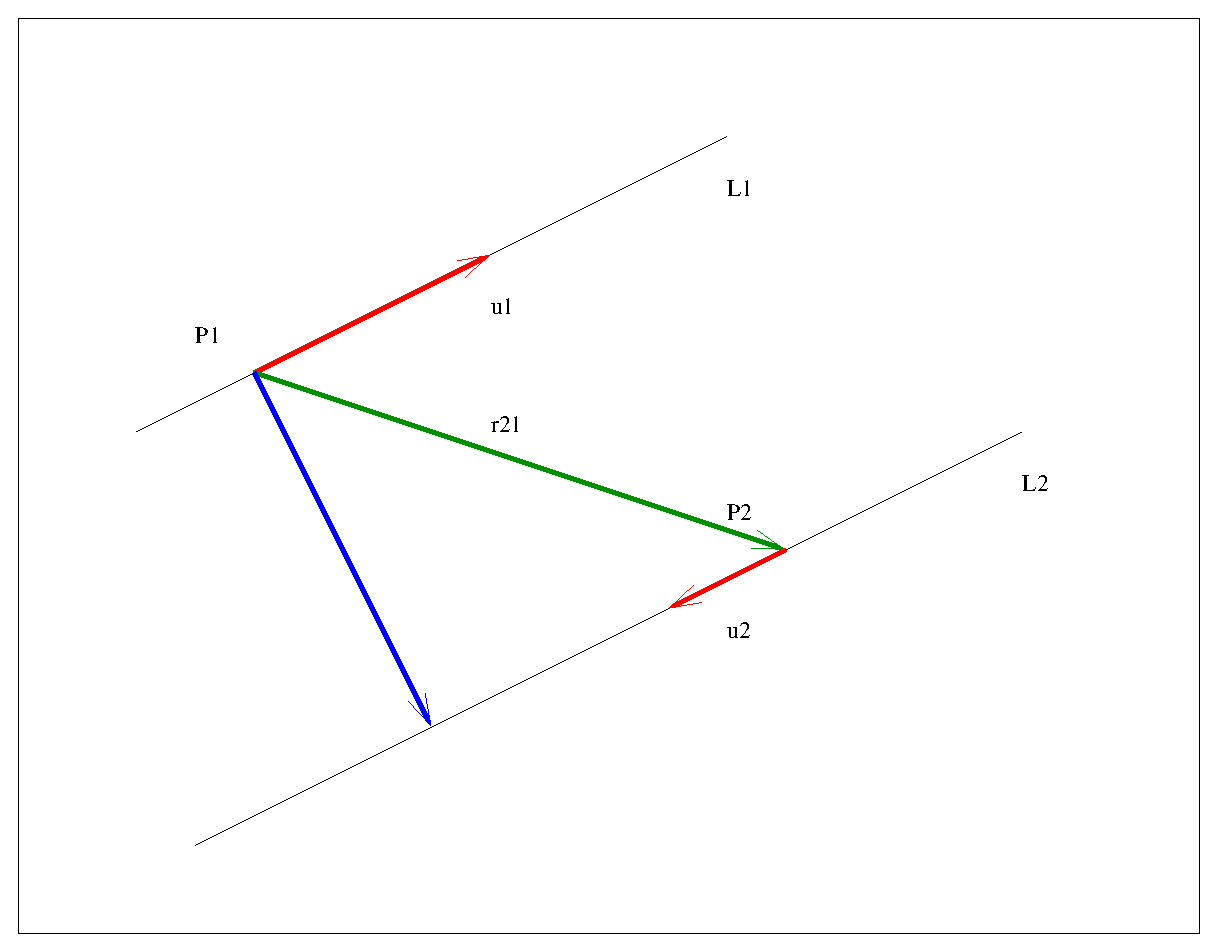
\includegraphics[height=2in]{../../modules/vectors/pictures/ok-distance_parallel_lines.eps}
    \end{figure}
\end{columns}

\end{frame}
\subsection{Angle Between Lines}
\begin{frame}
\frametitle{Angle between lines}

\begin{columns}
\column{0.4\textwidth}
\psfrag{L1}{$L_1$}
\psfrag{L2}{$L_2$}
\psfrag{P1}{$P_1$}
\psfrag{P2}{$P_2$}
\psfrag{u1}{$\textbf{u}_1$}
\psfrag{u2}{$\textbf{u}_2$}
\psfrag{a}{$\alpha$}
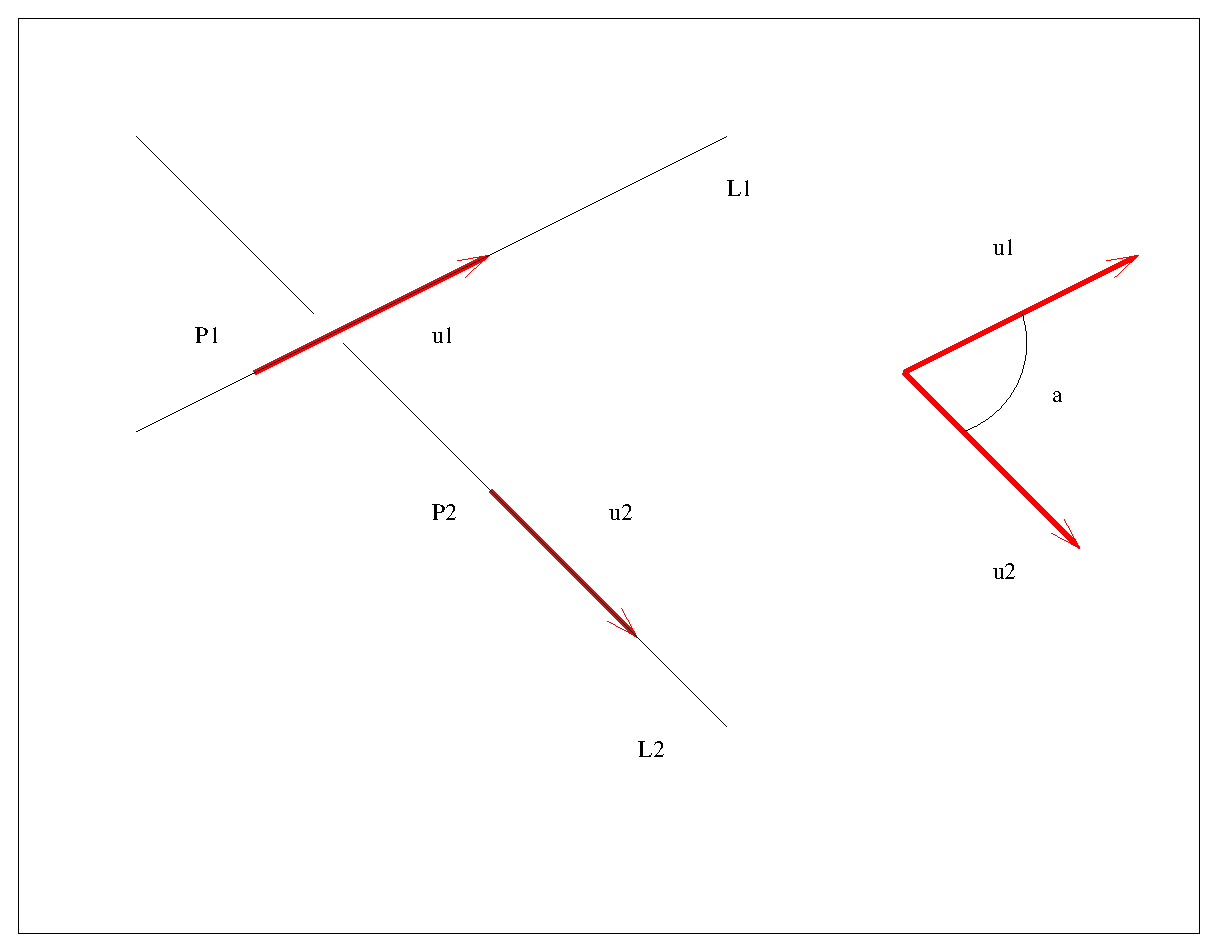
\includegraphics[height=1.4in]{../../modules/vectors/pictures/ok-angle_line_line.eps}
\column{0.6\textwidth}
\begin{itemize}
\item Given: lines $L_1: \quad \textbf{r}= \textbf{r}_1+t\textbf{u}_1 \qquad L_2: \quad \textbf{r}= \textbf{r}_2+s\textbf{u}_2$
\item Goal: find angle between $L_1$ and $L_2$.
\end{itemize}
\alert<1->{Perpendicular} lines
\uncover<2->{
$L_1 \bot L_2$ $\Longleftrightarrow$
$\textbf{u}_1 \bot \textbf{u}_2$ $\Longleftrightarrow$
$$\boxed{\textbf{u}_1 \cdot \textbf{u}_2 = 0}$$}
\uncover<3->{
\alert<1->{Angle} between lines}
\uncover<4->{
$\alpha$: angle between $L_1$, $L_2$ $\Longleftrightarrow$ 
$\alpha$: acute angle $\textbf{u}_1$, $\textbf{u}_2$}
\uncover<5->{$\Longleftrightarrow$
$$\boxed{\alpha = \arccos\left( \frac{|\textbf{u}_1 \cdot \textbf{u}_2|}{|\textbf{u}_1| \, |\textbf{u}_2|}\right) }$$}
\end{columns}
\end{frame}
\subsection{Distance Between Skew Lines}
\begin{frame}
\frametitle{Distance between lines}
\begin{columns}
\column{0.4\textwidth}
    \only<1>{\begin{figure}
        \psfrag{L1}{$L_1$}
        \psfrag{L2}{$L_2$}
        \psfrag{P1}{$P_1$}
        \psfrag{P2}{$P_2$}
        \psfrag{n}{$\textbf{n}$}
        \psfrag{r21}{$\textbf{r}_2-\textbf{r}_1$}
        \psfrag{u1}{$\textbf{u}_1$}
        \psfrag{u2}{$\textbf{u}_2$}
        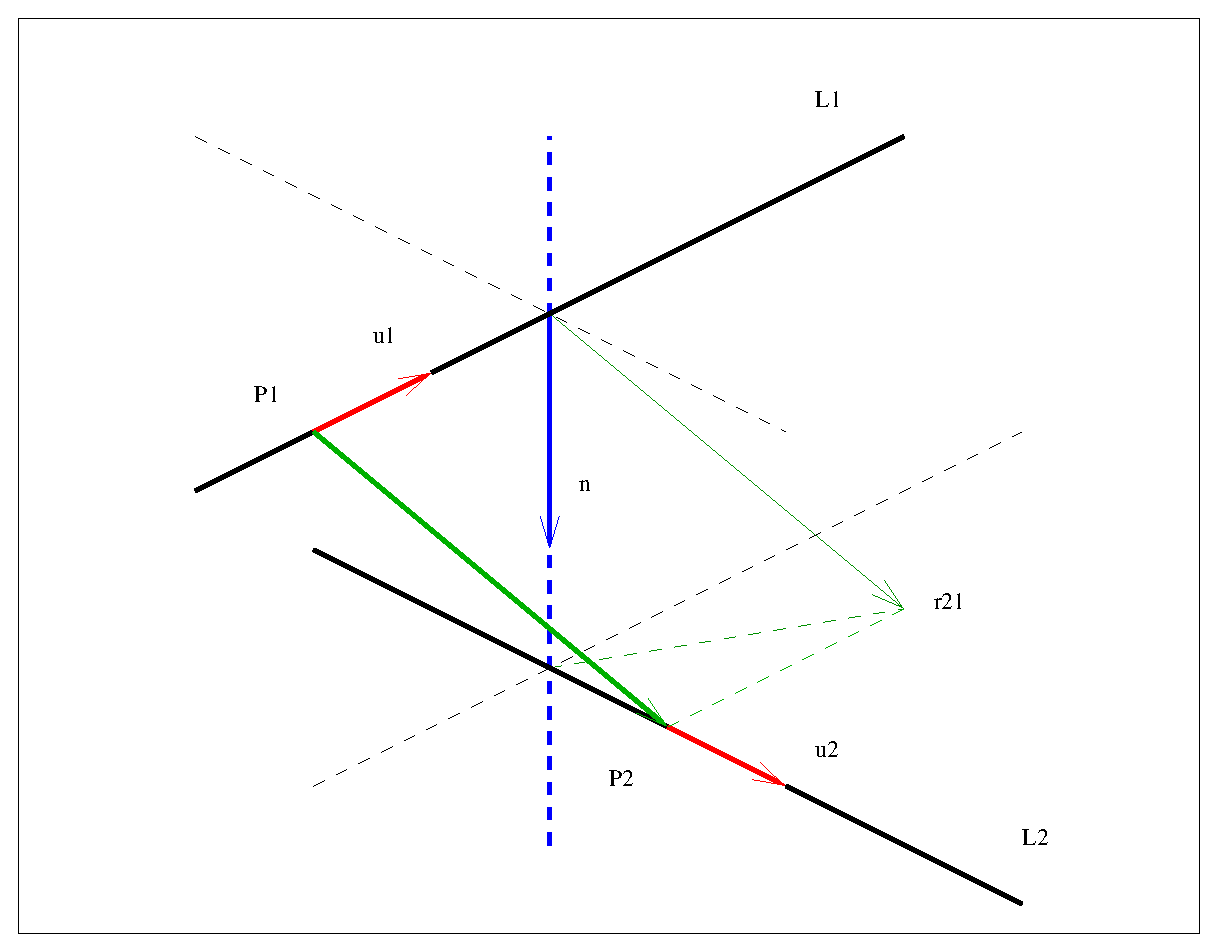
\includegraphics[height=1.4in]{../../modules/vectors/pictures/ok-distance_skew_lines.eps}
    \end{figure}}
    \only<2>{\begin{figure}
        \psfrag{L1}{$L_1$}
        \psfrag{L2}{$L_2$}
        \psfrag{P1}{$P_1$}
        \psfrag{P2}{$P_2$}
        \psfrag{n}{$\textbf{n}$}
        \psfrag{r21}{$\textbf{r}_2\!-\!\textbf{r}_1$}
        \psfrag{u1}{$\textbf{u}_1$}
        \psfrag{u2}{$\textbf{u}_2$}
        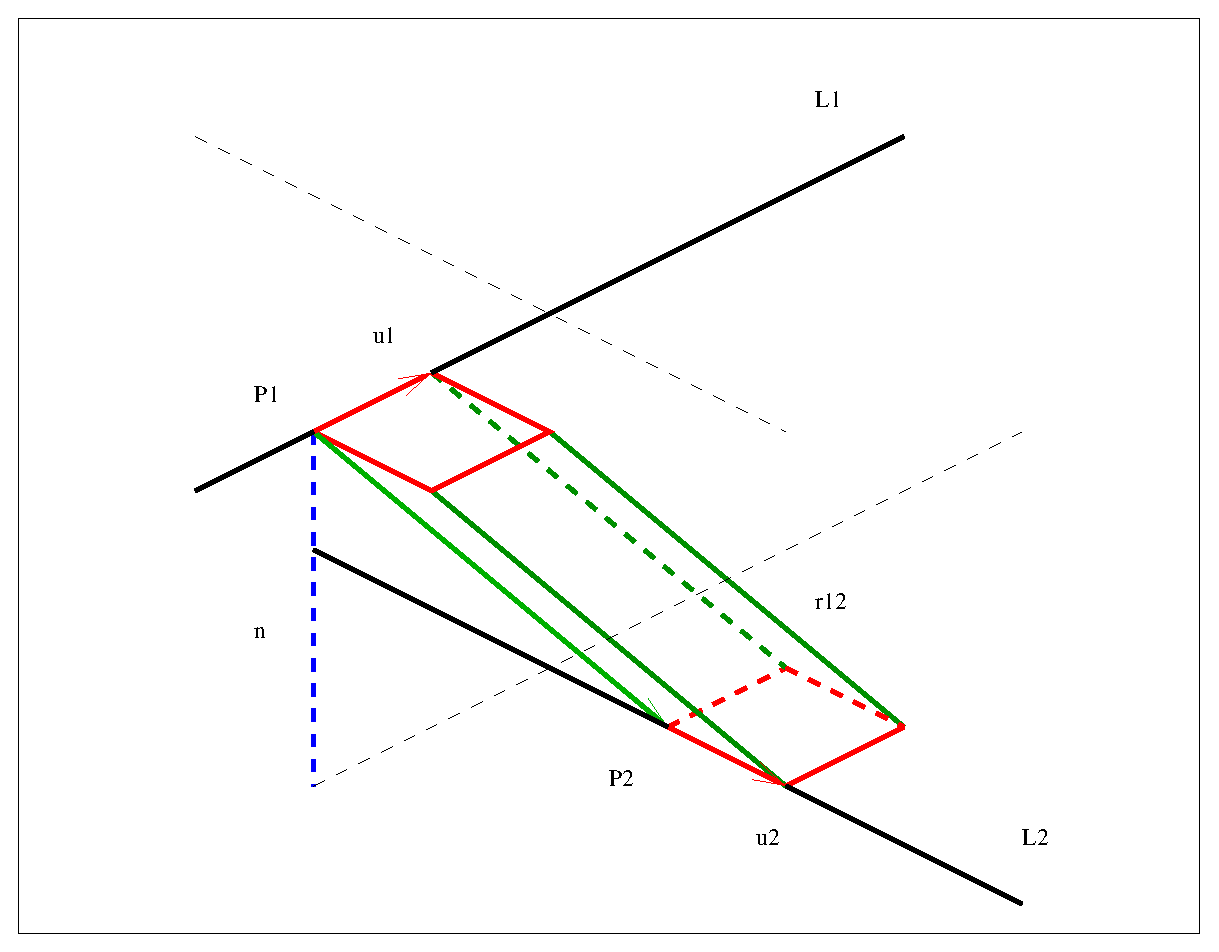
\includegraphics[height=1.4in]{../../modules/vectors/pictures/ok-distance_skew_lines_box.eps}
    \end{figure}
    }
\column{0.6\textwidth}
\begin{itemize}
\item Given: lines $L_1: \quad \textbf{r}= \textbf{r}_1+t\textbf{u}_1 \qquad L_2: \quad \textbf{r}= \textbf{r}_2+s\textbf{u}_2$
\item Goal: find distance between the lines (shortest distance between points on each line).
\end{itemize}


\end{columns}
\alert<1->{Skew lines}: $\textbf{n} = \textbf{u}_1 \times \textbf{u}_2 \neq \textbf{0}$. \alert<1->{Distance}:
$$d(L_1,L_2)  = |\textbf{\text{proj}}_{\bm{n}} (\textbf{r}_2-\textbf{r}_1)| = \boxed{\frac{|(\textbf{r}_2-\textbf{r}_1)\cdot \textbf{n}|}{|\textbf{n}|}}= \frac{|(\textbf{r}_2-\textbf{r}_1)\cdot (\textbf{u}_1\times \textbf{u}_2)|}{|\textbf{u}_1\times \textbf{u}_2|}$$
\alert<1>{Intersecting} lines: $d(L_1,L_2)=0$.
$$\textbf{u}_1\times \textbf{u}_2 \neq \textbf{0}$$
$$(\textbf{r}_2-\textbf{r}_1) \cdot (\textbf{u}_1\times \textbf{u}_2) = 0$$
\end{frame}

\subsection{Distance Between Plane and Parallel Line}
\begin{frame}
\frametitle{Distance between parallel line and plane}
\begin{columns}
\column{0.4\textwidth}
\psset{xunit=2cm, yunit=2cm}
\begin{pspicture}(-1.2, -1.2)(2,2)
\renewcommand{\fcScreen}{[-4 -1 -1] 0}
\tiny 
\fcParallelogramIIId{[-1 -1 0]}{[1 -1 0]}{[-1 1 0]}
\fcPutIIId{[-1 1 0]}{$\mathcal P$}
\fcPerpendicularIIId[linestyle=dotted]{[0.5 -0.7 0 ]}{[0 0.5 0] [0 0.5 1]}{0.2}
\fcLineIIId{[0 -1 1 ]}{[0 1 1]}
\fcDotIIId{[0 0.5 1]}
\fcPutIIId[b]{[0 0.5 1]}{$P_1(\fcv r_1)$}

\fcLineIIId[arrows=->, linecolor=blue]{[0 0.5 0]}{[0 0.5 1]}
\fcPutIIId[l]{[0 0.5 0.5]}{$\begin{array}{l} \fcv{orth}_{\fcv u}(\fcv r_1-\fcv r_0) =\\\fcv{proj}_{\fcv n}(\fcv r_1-\fcv r_0) \end{array}$}

\fcPerpendicularIIId[arrows=<-, linecolor=red]{[0.5 -0.7 0.5]}{[0.5 -0.7 0]}{0.2}

\fcDotIIId{[0.5 -0.7 0]}
\fcPutIIId[t]{[0.5 -0.7 -0.1]}{$P_0(\fcv r_0)$}
\fcLineIIId[arrows=->, linecolor=green]{[0 -0.7 0]}{[0 0.5 1]}
\fcPutIIId[tl]{[0 -0.1 0.5]}{$\fcv r_1-\fcv r_0$}

\fcLineIIId[linestyle=dotted]{[0.5 -0.7 0]}{[0.5 -0.7 0.9]}



\fcLineIIId[arrows=->, linecolor=red]{[0 -0.5 1]}{[0 0 1]}
\fcPutIIId[t]{[0 -0.25 0.9]}{$\fcv u$}


\fcPutIIId[r]{[0 -1 1]}{$L~~$}

\end{pspicture}
\column{0.6\textwidth}
\begin{itemize}
\item Given: line $L: \quad \fcv{r}= \fcv{r}_1+t\fcv{u}$,
\item plane $\mathcal{P}: \quad (\fcv{r}-\fcv{r}_0) \cdot \fcv{n} = 0$.
\item The plane and the line \alert<2>{are parallel,} \uncover<2->{i.e. $\fcv{u} \cdot \fcv{n} = 0$.}
\item Goal: find distance between the the two.
\end{itemize}

\end{columns}

\uncover<3->{
\alert<1->{Distance} from $L$ to $\mathcal{P}$:
$d(L,\mathcal{P}) = d(P_1,\mathcal{P})$}
\uncover<4->{
\[
\begin{array}{rcl}
d(L,\mathcal{P})&=&\displaystyle|\fcv{\text{orth}}_{\bm{u}}(\fcv{r}_1-\fcv{r}_0)| =
\fcv{\text{proj}}_{\bm{n}} (\fcv{r}_1-\fcv{r}_0)| \\~\\
d(L,\mathcal{P}) &=&\displaystyle \frac{|(\fcv{r}_1-\fcv{r}_0) \times \fcv{u}|}{|\fcv{u}|} =
\alert<1->{\frac{|(\fcv{r}_1-\fcv{r}_0)\cdot \fcv{n}|}{|\fcv{n}|}}
\end{array}
\]
}
\end{frame}

\subsection{Angle Between Plane and Line}
\begin{frame}
\frametitle{Angle between line and plane}
\begin{columns}
\column{0.4\textwidth}
        \psfrag{L}{$L$}
        \psfrag{cP}{$\mathcal{P}$}
        \psfrag{P0}{$P_0(\fcv{r}_0)$}
        \psfrag{P1}{$P_1(\fcv{r}_1)$}
        \psfrag{P2}{$P_2$}
        \psfrag{a}{$\alpha$}
        \psfrag{orth}{$\fcv{\text{orth}}_{\bm{n}}\fcv{u}$}
        \psfrag{u}{$\fcv{u}$}
        \psfrag{n}{$\fcv{n}$}
        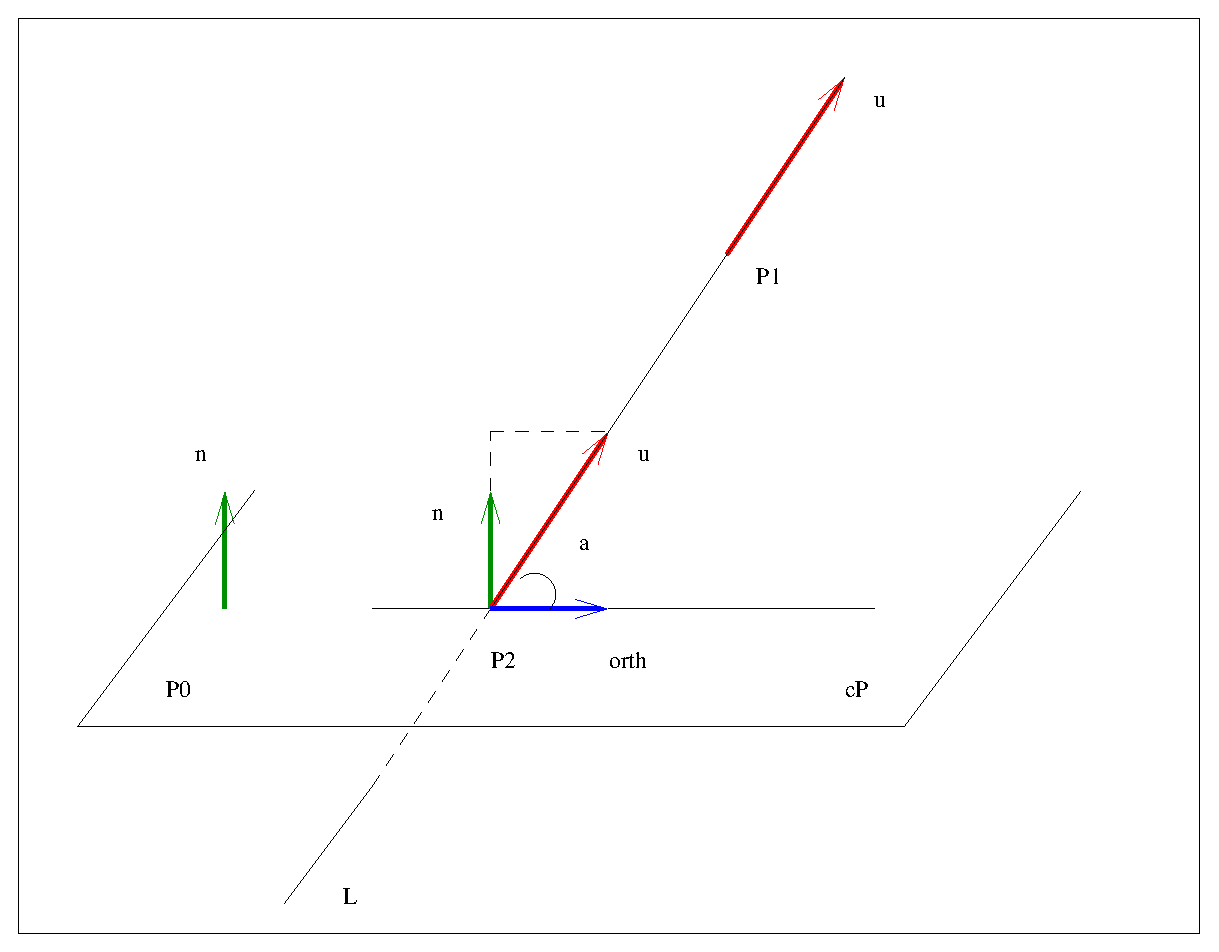
\includegraphics[height=1.4in]{../../modules/vectors/pictures/ok-angle_line_plane.eps}
    
\column{0.6\textwidth}
\begin{itemize}
\item Given: line $L: \quad \fcv{r}= \fcv{r}_1+t\fcv{u}$,
\item plane $\mathcal{P}: \quad (\fcv{r}-\fcv{r}_0) \cdot \fcv{n} = 0$.
\item Goal: Find angle between line and plane.
\end{itemize}
\end{columns}
Line \alert<1->{perpendicular} to plane
\uncover<2->{
$L \bot \mathcal{P}$ $\Longleftrightarrow$
$\fcv{u} \| \fcv{n}$ $\Longleftrightarrow$ 
$\boxed{\fcv{u} \times \fcv{n} = \fcv{0}}$
}

\uncover<3->{
\alert<1->{Angle} between line and plane $\alpha$: angle between $L$, $\mathcal{P}$ $\Longleftrightarrow$ $\alpha$: acute angle $\fcv{u}$, $\fcv{\text{orth}}_{\bm{n}}\fcv{u}$} 
\uncover<4->{
$\Longleftrightarrow$
$\boxed{\alpha = \arcsin\left( \frac{|\fcv{u} \cdot \fcv{n}|}{|\fcv{u}| \, |\fcv{n}|}\right) }$
}

\uncover<5->{\alert<1>{Intersection}:}

\uncover<6->{
$\begin{array}{rcl}
(\fcv{r}_1+t\fcv{u}-\fcv{r}_0) \cdot \fcv{n} &=& 0\\
(\fcv{r}_1-\fcv{r}_0)\cdot \fcv{n} + t \fcv{u} \cdot \fcv{n} &=& 0
\end{array}
$

Solve for $t$.
}
\end{frame}
\subsection{Angle Between Plane and Line}
\begin{frame}\frametitle{Intersection between line and plane}
\begin{columns}
\column{0.4\textwidth}
\psset{xunit=2cm, yunit=2cm}
\begin{pspicture}(-1.2, -0.7)(2,1.33)
\renewcommand{\fcScreen}{[-4 -1 -1] 0}
\tiny
\fcParallelogramIIId{[-1 -1 0]}{[1 -1 0]}{[-1 1 0]}
\fcPutIIId{[-1 1 0]}{$\mathcal P$}
%\fcLineIIId[arrows=->, linecolor=blue]{[0 0.5 0]}{[0 0.5 1]}
%\fcLineIIId[arrows=->, linecolor=red]{[0.5 -0.7 0]}{[0.5 -0.7 0.5]}
%\fcPutIIId[r]{[0.5 -0.7 0.25]}{$\fcv n~~$}



\fcLineIIId[arrows=->, linecolor=blue]{[0.5 -0.7 0]}{[0 0.5 1]}
\fcPutIIId[tl]{[0.25 -0.1 0.5]}{$ \alert<5>{\fcv u}$}
\fcLineIIId[linestyle=dotted]{[0.56 -0.844 -0.12]}{[0.5 -0.7 0]}
\fcLineIIId{[0.65 -1.06 -0.3]}{[0.56 -0.844 -0.12]}
\fcLineIIId{[0 0.5 1]}{[-0.15 0.86 1.3]}
\fcPutIIId[tl]{[0.65 -1.06 -0.3]}{$~~L$}
\fcDotIIId{[-0.15 0.86 1.3]}
\fcDotIIId{[0.5 -0.7 0]}

\end{pspicture}
\column{0.6\textwidth}
\begin{itemize}
\item Given: line $L: \quad\alert<6>{ \fcv{r}= \fcv{r}_1+t\fcv{u}}$,
\item $\fcv r_1=( x_1, y_1, z_1)$, $u=( p,q,r)$,
\item plane $\mathcal{P}: \alert<12>{\alert<4>{ax +by +cz} \alert<5>{ -d}=0}$.
\item Goal: find the intersection between line and plane.
\end{itemize}
\end{columns}
\uncover<2->{Let $P_0(\fcv r_0)$ be a point on the plane.} \uncover<3->{Then a point $P(\fcv r)$, $\fcv r=( x,y,z)$ is on the plane if
$
\alert<12>{( \alert<4,7>{\fcv r}\alert<5,8>{-\fcv r_0})\alert<4,5,8>{\cdot \fcv n}=0}.
$
} %uncover3
\uncover<6->{A point $P(\fcv r) $ \alert<6>{on the line} is of the form $\alert<6,7>{\fcv r=\fcv r_1+t\fcv u}$,} \uncover<7->{therefore $P$ lies on both the line and the plane if:
\[\begin{array}{rcl}
(\alert<7>{ \fcv{r}_1+t\fcv{u}}-\alert<8>{\fcv{r}_0})\alert<8>{ \cdot \fcv{n} }&=& 0\\
\uncover<9->{ (\fcv{r}_1-\fcv{r}_0)\cdot \fcv{n} + t \fcv{u} \cdot \fcv{n} &=& 0\\}
\uncover<10->{t&=& -\frac{(\fcv{r}_1-\fcv r_0)\cdot\fcv  n}{\fcv u \cdot \fcv n}\\}
\uncover<11->{\fcv r&= &\fcv r_1-\frac{\alert<12>{(\fcv{r}_1-\fcv r_0)\cdot\fcv  n}}{\fcv u \cdot \fcv n}\fcv u }\\
\uncover<12->{&=& ( x_1, y_1, z_1 )-\frac{\alert<12>{ ax_1 +by_1+cz_1-d}}{ap + bq +cr }( p,q, r)}
\end{array}
\]
}
\end{frame}

\subsection{Parallel Planes}
\begin{frame}
  \frametitle{Parallel planes}
\begin{columns}
\column{0.4\textwidth}
\begin{pspicture}(-0.2, -0.2)(2,2)
\tiny
\fcParallelogramIIId{[-1.5 -1.5 -1]}{[-1.5 1.5 -1]}{[1.5 -1.5 -1]}
\fcParallelogramIIId{[-1.5 -1.5 1]}{[-1.5 1.5 1]}{[1.5 -1.5 1]}
\fcPutIIId{[-1.5 -1.5 -1]}{$\mathcal P_1$}
\fcPutIIId{[-1.5 -1.5 1]}{$\mathcal P_2$}
\fcLineIIId{[-1 -1 -1]}{[1 1 -1]}
\fcLineIIId{[-1 -1 1]}{[1 1 1]}
\fcDotIIId{[1 1 1]}
\fcPutIIId[tl]{[1 1 0.9]}{$~~P_2$}
\fcDotIIId{[-1 -1 -1]}
\fcPutIIId[t]{[-1 -1 -1.1]}{$P_1$}
\fcLineIIId[linecolor=gray]{[-1 -1 -1]}{[-1 -1 0.73]}%
\fcLineIIId[linecolor=gray, linestyle=dotted]{[-1 -1 0.73]}{[-1 -1 1]}%
\fcPerpendicularIIId[arrows=<-, linecolor=red]{[-1 -1 0.1]}{[-1 -1 -1] [0 0 -1]}{0.2}%
\fcPutIIId[r]{[-1 -1 -0.45]}{$\fcv n_1~~$}

\fcPerpendicularIIId[linecolor=gray]{[1 1 0.73]}{[1 1 -1] [-1 -1 -1]}{0.2}%
\fcLineIIId[linecolor=gray, linestyle=dotted]{[1 1 0.73]}{[1 1 1]}%

\fcPerpendicularIIId[arrows=<-, linecolor=red]{[1 1 1.7]}{[1 1 1] [0 0 1]}{0.2}%
\fcPutIIId[l]{[1 1 1.35]}{$~~\fcv n_2$}

\fcLineIIId[linecolor=blue]{[-1 -1 -1]}{[0.53 0.53 0.53]}
\fcLineIIId[arrows=->, linecolor=blue, linestyle=dotted]{[0.53 0.53 0.53]}{[1 1 1]}
\fcPutIIId[l]{[0 0 0]}{$~~~\fcv r_2- \fcv r_1$}
\end{pspicture}
\column{0.6\textwidth}
\begin{itemize}
\item Given: planes $\begin{array}{rrcl}
\mathcal{P}_1:& (\textbf{r} - \alert<7>{\textbf{r}_1})\alert<7>{ \cdot \alert<6>{\textbf{n}_1}} &=& 0 \\
\mathcal{P}_2:& (\textbf{r} - \alert<7>{\textbf{r}_2}) \alert<7>{\cdot \alert<6>{\textbf{n}_2}} &=& 0
\end{array}.
$
\item Goal: Establish whether planes are parallel, find distance b-n planes.
\end{itemize}
\end{columns}
Planes are \alert<1->{parallel} \uncover<2->{$\mathcal{P}_1 || \mathcal{P}_2$ $\Leftrightarrow$ $\textbf{n}_1$, $\textbf{n}_2$ collinear $\Leftrightarrow$
$\boxed{\textbf{n}_1 \times \textbf{n}_2 = \textbf{0}}$. }

\uncover<3->{\alert<1->{Distance}:\quad
$d(\mathcal{P}_1,\mathcal{P}_2) = |\textbf{\text{proj}}_{\textbf{n}_1} (\textbf{r}_2-\textbf{r}_1)| \uncover<4->{=\boxed{\frac{|(\textbf{r}_2-\textbf{r}_1)\cdot \textbf{n}_1|}{|\textbf{n}_1|}}}$
} %uncover3

\uncover<5->{%
\noindent Assume $\alert<6>{ \fcv n_1=\fcv n_2=( a,b,c) }$
\uncover<6->{$\Rightarrow$ plane eq-ns:
$\begin{array}{r@{~}r@{~}c@{~}l}
\mathcal{P}_1 :& \alert<6>{a}x+\alert<6>{b}y+\alert<6>{c}z &=& \alert<7>{d_1}\\
\mathcal{P}_2 :& \alert<6>{a}x+\alert<6>{b}y+\alert<6>{c}z &=& \alert<7>{d_2}
\end{array}.$
}
\uncover<7->{
\[
\Rightarrow \boxed{d(\mathcal{P}_1,\mathcal{P}_2) = \frac{|\alert<7>{d_2-d_1}|}{\sqrt{a^2+b^2+c^2}}}
\]
}
}%uncover5
\end{frame}

\subsection{Angle Between Planes}
\begin{frame}
\frametitle{Angle between planes}
\begin{columns}
\column{0.35\textwidth}
\centering
\psset{xunit=1.2cm, yunit=1.2cm}
\begin{pspicture}(-2, -2)(2,2)
\tiny
\renewcommand{\fcScreenStyle}{x}
%\fcAxesIIId{2}{2}{2}
\fcParallelogramIIId[linecolor=green!30]{[1 0 -1]}{[1 1 -1]}{[0 0 0]}
\fcParallelogramIIId[linecolor=magenta!30]{[1 0 0]}{[1 1 0]}{[-1 0 0]}
\fcParallelogramIIId[linecolor=green!30]{[0 0 0]}{[-1 0 1]}{[0 1 0]}
\uncover<6->{
\fcParallelogramIIId[linecolor=cyan!30]{[1 0 -1]}{[1 0 1]}{[-1 0 -1]}
}
\fcParallelogramIIId[linecolor=green!30]{[1 -1 -1]}{[1 0 -1]}{[0 -1 0]}
\fcParallelogramIIId[linecolor=magenta!30]{[1 -1 0]}{[1 0 0]}{[-1 -1 0]}
\fcParallelogramIIId[linecolor=green!30]{[0 0 0]}{[0 -1 0]}{[-1 0 1]}

\uncover<6->{%
\fcPutIIId[b]{[0.8 0 1.1]}{$\mathcal P_3$}
\fcPolyLineIIId{[1 0 -1] [1 0 1] [-1 0 1]}
\fcLineIIId[linestyle=dashed]{[-1 0 1]}{[-1 0 -0.5]}
\fcPolyLineIIId{[-1 0 -0.5] [-1 0 -1] [-0.5 0 -1]}
\fcLineIIId[linestyle=dashed]{[-0.5 0 -1]}{[1 0 -1]}
}
\fcPolyLineIIId[linestyle=dashed]{[-1 -0.35 0] [-1 1 0] [0 1 0]}
\fcPolyLineIIId{[-1 -0.35 0] [-1 -1 0] [1 -1 0] [1 1 0] [0 1 0]}
\fcPolyLineIIId{[0 1 0] [-1 1 1] [-1 -1 1] [1 -1 -1] [1 1 -1] [0.33 1 -0.33]}%
\fcLineIIId[linestyle=dashed]{[0.33 1 -0.33]}{[0 1 0]}%
%\uncover<9->{%
%\fcPerpendicularIIId[arrows=<-, linecolor=red]{[1.7 0 0.3]}{[1 0 -1]}{0.2}%
%\fcDotIIId{[0.7 0 -0.7]}%
%\fcPutIIId[tl]{[0.7 0 -0.7]}{$~~P_1$}%
%\fcPutIIId[l]{[1.5 0 0]}{$~\fcv n_1$}
%}%
%\fcPerpendicularIIId[arrows=<-, linecolor=red]{[1 0 1]}{[-1 0 1]}{0.2}
\uncover<9->{%
\fcLineIIId[arrows=<-, linecolor=red]{[1 0 1]}{[0 0 0]}
\fcPutIIId[tl]{[0.85 0 0.85]}{$~~~~\fcv n_1$}%
}%
%\uncover<9->{%
%\fcPerpendicularIIId[arrows=<-, linecolor=red]{[0.8 0.8 0.8]}{[0.8 0.8 0] [0.6 0.8 0]}{0.2}%
%\fcDotIIId{[0.8 0.8 0]}
%\fcPutIIId[bl]{[0.8 0.8 0]}{$~~P_2$}
%\fcPutIIId[bl]{[0.8 0.8 0.5]}{$~~\fcv n_2$}
%}%

\fcLineIIId[linecolor=gray]{[0 -1 0]}{[0 1 0]}
\fcPutIIId[b]{[0 -1 0.1]}{$L$}
%\fcPerpendicularIIId[arrows=<-, linecolor=red]{[0 0 0.8]}{[-1 0 0]}{0.1}
\uncover<9->{%
\fcLineIIId[arrows=<-, linecolor=red]{[0 0 0.8]}{[0 0 0]}
\fcPutIIId[bl]{[0 0 0.5]}{$~~\fcv n_2$}
}%
\fcPolyLineIIId{[-0.5 0 0.5] [0 0 0]}%
\fcLineIIId[linestyle=dashed]{[0 0 0]}{[0.2 0 -0.2]}%
\uncover<3-4>{%
\fcPerpendicularIIId{[-0.5 0 0.5]}{[0 1 0]}{0.2}%
}%
\uncover<3->{%
\fcDotIIId{[-0.5 0 0.5]}%
\fcPutIIId[b]{[-0.5 0 0.6]}{$Q_1$}
}%

\fcLineIIId[linestyle=dashed]{[0 0 0]}{[-0.7 0 0]}%
\fcLineIIId{[0 0 0]}{[0.7 0 0]}%
\uncover<4->{%
\fcDotIIId{[-0.7 0 0]}%
\fcPutIIId[t]{[-0.7 0 -0.1]}{$Q_2$}
}%
\uncover<4>{%
\fcPerpendicularIIId[linestyle=dashed]{[-0.7 0 0]}{[0 1 0]}{0.2}%
}%
\uncover<5->{%
\fcAngleIIId[linecolor=blue]{[-1 0 1]}{[-1 0 0]}{0.3}%
\fcPutIIId[rb]{[-0.3 0 0.1]}{$\alpha$}%
}%
\uncover<11->{\fcAngleIIId[linecolor=blue]{[0 0 1]}{[1 0 1]}{0.3}}%
\uncover<13->{%
\fcLineIIId[arrows=->, linecolor=blue]{[0 0 0]}{[0 -0.8 0]}%
\fcPutIIId[l]{[0 -0.5 0]}{$~\fcv u$}%
}%
\fcPutIIId[tr]{[-1 -1 0]}{$\mathcal P_2$}
\fcPutIIId[tr]{[-1 -1 1]}{$\mathcal P_1$}
%\fcParallelogramHollowIIId{[-1 -1 0]}{[1 -1 0]}{[-1 1 0]}
%\fcParallelogramHollowIIId{[1 -1 -1]}{[1 1 -1]}{[-1 -1 1]}
\end{pspicture}
\uncover<6->{%
\psset{xunit=1cm, yunit=1cm}
\begin{pspicture}(-0.2, -0.2)(0.2, 0.2)
\tiny
\renewcommand{\fcScreen}{[0 1 0] 0}
\fcBoundingBox{-1.5}{-1.5}{1.5}{1.5}
\fcParallelogramIIId[linecolor=cyan!30]{[1 0 -1]}{[1 0 1]}{[-1 0 -1]}
\fcPutIIId[t]{[0 0 -0.1]}{$O$}
\fcPutIIId[b]{[0.8 0 1.1]}{$\mathcal P_3$}
\uncover<9->{%
\fcPutIIId[bl]{[0 0 0.6]}{$~~\fcv n_2$}
\fcPutIIId[tl]{[0.85 0 0.85]}{$~~\fcv n_1$}%
}%uncover9
\uncover<9>{%
\fcLineIIId[arrows=<-, linecolor=red]{[0 0 0.8]}{[0 0 0]}%
\fcLineIIId[arrows=<-, linecolor=red]{[1 0 1]}{[0 0 0]}%
}%uncover9
\uncover<10->{%
\fcPerpendicularIIId[arrows=<-, linecolor=red]{[0 0 0.8]}{[1 0 0]}{0.12}%
\fcPerpendicularIIId[arrows=<-, linecolor=red]{[1 0 1]}{[1 0 -1]}{0.2}%
}%
\fcLineIIId{[0 0 0]}{[-0.7 0 0]}%
\fcPolyLineIIId{[-0.5 0 0.5] [0 0 0]}%
\fcAngleIIId[linecolor=blue]{[-1 0 1]}{[-1 0 0]}{0.35}%
\fcPutIIId[rb]{[-0.3 0 0.15]}{$\alpha$}%
\uncover<11->{%
\fcAngleIIId[linecolor=blue]{[0 0 1]}{[1 0 1]}{0.35}%
\fcPutIIId[lb]{[0.1 0 0.35]}{$\alpha~~$}%
}%
\fcDotIIId{[-0.5 0 0.5]}%
\fcPutIIId[b]{[-0.5 0 0.6]}{$Q_1$}
\fcDotIIId{[-0.7 0 0]}%
\fcPutIIId[t]{[-0.7 0 -0.1]}{$Q_2$}
\end{pspicture}
}%
\vskip 6cm
\column{0.65\textwidth}
\begin{itemize}
\item Given: planes 
$\begin{array}{rrcl}
\mathcal{P}_1:&  (\fcv{r} - \fcv{r}_1) \cdot \alert<9>{\fcv{n}_1 }&=& 0 \\
\mathcal{P}_2:& (\fcv{r} - \fcv{r}_2) \cdot \alert<9>{\fcv{n}_2} &=& 0
\end{array}
$
\item Goal: \alert<4>{define} and find the angle between the two planes.
\only<1-6>{%
\item<2-> Let $L$ - intersection line of two planes.
\item<3-> In $\mathcal P_1$, drop perpendicular from arbitrary point $Q_1$ to $L$.
\item<4-> In $\mathcal P_2$, raise a perpendicular from the perpendicular heel.
\item<5-> \alert<4>{Define angle $\alpha$} b-n $\mathcal P_1, \mathcal P_2$ = acute angle b-n two perpendiculars.
}%
\item<6-> \alert<6,7>{Consider the plane $\mathcal P_3$ spanned by the two constructed perpendiculars.}

\only<1-6>{%
\vskip 0.57cm
}%
\only<7->{%
\item<8-> $\mathcal P_3$ is orthogonal to $L$.
\item<9-> $\Rightarrow$ $\mathcal P_3$ contains the normal vectors $\fcv n_1$, $\fcv n_2$.
\item<10-> $\fcv n_1\perp \fcv O\fcv Q_{1}$ and $\fcv n_2\perp \fcv O\fcv Q_{2}$.
\item<11-> 
$
\begin{array}{rcl}
\alpha &=& \text{acute} \angle (\fcv{n}_1,\fcv{n}_2) \\
\alpha &=&\arccos{\left( \frac{|\fcv{n}_1 \cdot \fcv{n}_2|}{|\fcv{n}_1|\, |\fcv{n}_2|}\right)}
\end{array}
$
\item<12-> $\perp$ planes: $\Rightarrow$ $\alpha = \frac{\pi}{2} \Longleftrightarrow \boxed{\fcv{n}_1 \cdot \fcv{n}_2 = 0}$.
\item<13-> Direction of $L$ is $\fcv{u} = \fcv{n}_1 \times \fcv{n}_2$.
}%onlyr<7->
\end{itemize}

\vfill

\end{columns}
\vskip 5cm

\end{frame}
} %end lecture

% begin lecture
\lect{September 2014}{Lecture  5}{5}{
\section{Polar Coordinates}
% begin module polar-intro
\begin{frame}[t]
\frametitle{Polar Coordinates}
\begin{itemize}
\item<1->  The polar coordinates system is an alternative to the Cartesian coordinates system.
%\item  Instead of specifying horizontal distance and vertical distance, we specify angle and distance from the origin.
\item<2->  Choose a point in the plane called $O$ (the origin).
\item<3->  Draw a ray starting at $O$. The ray is called the polar axis.  This ray is usually drawn horizontally to the right.
\end{itemize}
\begin{columns}[c]
\column{.5\textwidth}
\psset{xunit=5cm, yunit=5cm}
\begin{pspicture}(-0.2, -0.2)(1.500000,0.6)
\tiny
%force a boudning box:
\psline[linecolor=red!1](-0.1, -0.1)(-0.21,0.2)
\psline[linecolor=red!1](1.1, 0.6)(1.1,0.61)

\uncover<5->{
%Calculator input: plotCurve{}(1/5 \cos{}t, 1/5 \sin{}t, 0, 1/6 \pi)
\parametricplot[arrows=->, linecolor=red, plotpoints=1000] {0}{0.523599}{t 57.29578 mul cos 0.2 mul t 57.29578 mul sin 0.2 mul }
\psline[linecolor=blue](0,0)(0.866025404, 0.5)
\rput(0.22, 0.06){$\alert<5>{\theta}$}
}

\uncover<4->{
\fcFullDotBlue{0.866025404}{0.5}
\rput[l](0.88, 0.5){$P\uncover<7->{\alert<7>{(r,\theta)}}$}
}

\uncover<2->{
\fcFullDotBlue{0}{0}
\rput(-0.1, 0){$O$}
}
\uncover<6->{
\rput(0.4, 0.3){$\alert<6>{r}$}
}
\uncover<3->{
\psline{->}(0,0)(1,0)
\rput (0.5, -0.05){polar axis}
}
\end{pspicture}

\vspace{1cm}

%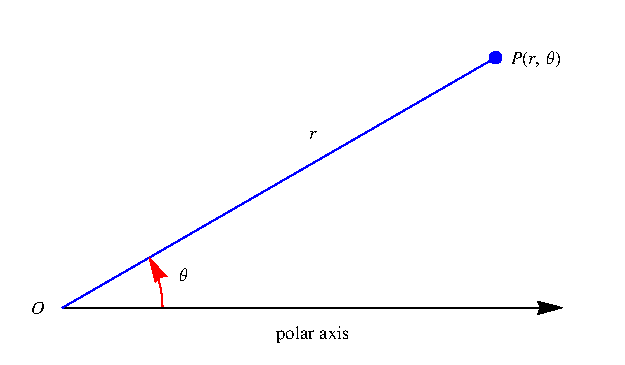
\includegraphics[height=4cm]{polar-curves/pictures/11-03-polar.pdf}%
\column{.5\textwidth}
\begin{itemize}
\only<1-7>{\item<4->  Let $P$ be a point in the plane.
\item<5->  Let $\theta$ denote the angle between the polar axis and the line $OP$.
\item<6->  Let $r$ denote the length of the segment $OP$.
\item<7->  Then $P$ is represented by the ordered pair $(r, \theta )$.
}
\only<8->{
\item<8->  The letters $(x,y)$ imply Cartesian coordinates and the letters $(r, \theta)$- polar. \uncover<9->{When we use other letters, it should be clear from context whether we mean Cartesian or polar coordinates.} \uncover<10->{If not, one must request clarification.}
}
\end{itemize}
\end{columns}
\end{frame}
% end module polar-intro

% begin module polar-questions
\begin{frame}
\begin{enumerate}
\item<1-| alert@2>  What if $\theta$ is negative?
\item<1-| alert@3>  What if $r$ is negative?
\item<1-| alert@4>  What if $r$ is $0$?
\end{enumerate}
\begin{columns}[T]
\column{.5\textwidth}
\uncover<2->{
\psset{xunit=2cm, yunit=2cm}
\begin{pspicture}(-0.9, -1.2)(2,0.2)
\tiny
%force a boudning box:
%\psline[linecolor=red!1](-0.1, -0.1)(-0.21,0.2)
%\psline[linecolor=red!1](1.1, 0.6)(1.1,0.61)
\fcFullDotBlue{0}{0}

%Calculator input: plotCurve{}(1/10 \cos{}t, 1/10 \sin{}t, 0, -3/4 \pi)
\parametricplot[arrows=->, linecolor=\fcColorGraph, plotpoints=100]{0} {-2.35619} {t 57.29578 mul cos 0.3000000 mul t 57.29578 mul sin 0.3000000 mul }
\rput[t] (0,-0.1){$O$}
\rput[l](0.3, -0.2){$\theta=-\frac{3\pi}{4}$}

\psline{->}(0,0)(1.5,0)
\psline[linecolor=blue](0,0)(-0.707106781, -0.707106781)
\fcFullDotBlue{-0.707106781}{-0.707106781}
\rput[tl](-0.6, -0.7){$\begin{array}{l}(r,\theta)=\left(1, -\frac{3\pi}{4}\right)\\ (x,y)=\left(-\frac{\sqrt{2}}2, -\frac{\sqrt{2}}2 \right) \end{array}$}
\end{pspicture}
}

\uncover<3->{
\psset{xunit=2cm, yunit=2cm}
\begin{pspicture}(-0.9, -1.5)(2.2,1)
\tiny
%force a boudning box:
%\psline[linecolor=red!1](-0.1, -0.1)(-0.21,0.2)
%\psline[linecolor=red!1](1.1, 0.6)(1.1,0.61)
\fcFullDotBlue{0}{0}

\parametricplot[arrows=->, linecolor=\fcColorGraph, plotpoints=100]{0} {0.523598776 } {t 57.29578 mul cos 0.3000000 mul t 57.29578 mul sin 0.3000000 mul }
\parametricplot[arrows=->, linecolor=brown, plotpoints=100]{0} {3.665191429 } {t 57.29578 mul cos 0.25 mul t 57.29578 mul sin 0.25 mul }

\rput[t] (0,-0.1){$O$}

\psline{->}(0,0)(1.5,0)
\psline[linecolor=blue](0,0)(0.866025404, 0.5)
\fcFullDotBlue{0.866025404}{0.5}
\rput[tl](-0.75, -0.5){
$(-r, \theta)$
}
\fcFullDotBlue{-0.866025404}{-0.5}
\psline[linecolor=blue, linestyle=dashed](0,0) (-0.866025404,-0.5)
\rput[tl](0.6, 0.7){$(r, \theta) $}
\end{pspicture}
}
%\ \uncover<2->{%
%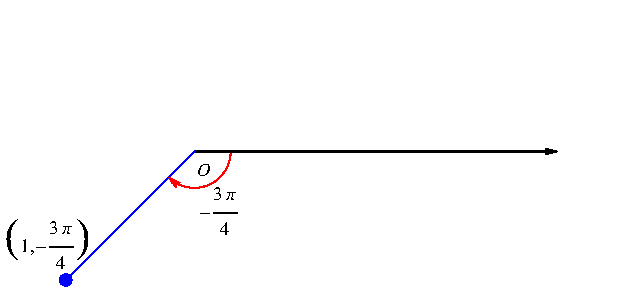
\includegraphics[height=3cm]{polar-curves/pictures/11-03-ex1b.pdf}%
%}%
%\ \uncover<3->{%
%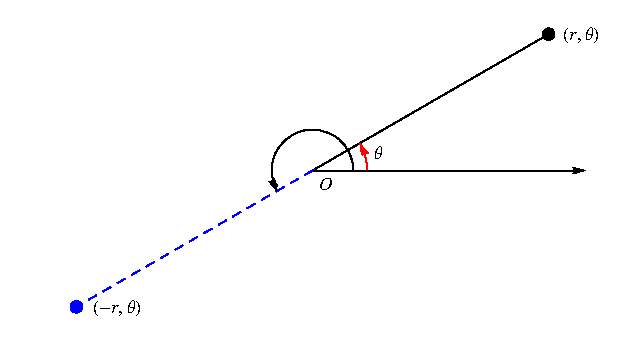
\includegraphics[height=3cm]{polar-curves/pictures/11-03-negativer.pdf}%
%}%
\column{.5\textwidth}
\begin{enumerate}
\item<2-| alert@2>  Positive angles $\theta$ are measured in the counterclockwise direction from $O$.  Negative angles are measured in the clockwise direction.
\item<3-| alert@3>  Points with polar coordinates $(-r, \theta)$ and $(r, \theta)$ lie on the same line through $O$ and at the same distance from $O$, but on opposite sides.
\item<4-| alert@4>  If $r = 0$, then $(0, \theta)$ represents $O$ for all values of $\theta$.
\end{enumerate}
\end{columns}
\end{frame}
% end module polar-questions

% begin module polar-many-representations
\begin{frame}
\begin{columns}[c]
\column{.5\textwidth}
\uncover<1->{
\psset{xunit=2cm, yunit=2cm}
\begin{pspicture}(-0.9, -1.1)(2,0.5)
\tiny
%force a boudning box:
%\psline[linecolor=red!1](-0.1, -0.1)(-0.21,0.2)
%\psline[linecolor=red!1](1.1, 0.6)(1.1,0.61)
\fcFullDotBlue{0}{0}

%Calculator input: plotCurve{}(1/10 \cos{}t, 1/10 \sin{}t, 0, -3/4 \pi)
\parametricplot[arrows=->, linecolor=\fcColorGraph, plotpoints=100]{0} {3.926990817} {t 57.29578 mul cos 0.3000000 mul t 57.29578 mul sin 0.3000000 mul }
\rput[t] (0,-0.1){$O$}
\rput[l](0.3, 0.3){$\theta=\frac{5\pi}{4}$}

\psline{->}(0,0)(2,0)
\psline[linecolor=blue](0,0)(-0.707106781, -0.707106781)
\fcFullDotBlue{-0.707106781}{-0.707106781}
\rput[tl](-0.6, -0.7){$(r,\theta)=\left(1, \frac{5\pi}{4}\right)$}
\end{pspicture}
}
\uncover<2->{
\psset{xunit=2cm, yunit=2cm}
\begin{pspicture}(-0.9, -1.1)(2,0.5)
\tiny
%force a boudning box:
%\psline[linecolor=red!1](-0.1, -0.1)(-0.21,0.2)
\psline[linecolor=red!1](1.1, 0.5)(1.1,0.51)
\fcFullDotBlue{0}{0}

%Calculator input: plotCurve{}(1/10 \cos{}t, 1/10 \sin{}t, 0, -3/4 \pi)
\parametricplot[arrows=->, linecolor=\fcColorGraph, plotpoints=100]{0} {-2.35619} {t 57.29578 mul cos 0.3000000 mul t 57.29578 mul sin 0.3000000 mul }
\rput[t] (0,-0.1){$O$}
\rput[l](0.3, -0.2){$\theta=-\frac{3\pi}{4}$}

\psline{->}(0,0)(2,0)
\psline[linecolor=blue](0,0)(-0.707106781, -0.707106781)
\fcFullDotBlue{-0.707106781}{-0.707106781}
\rput[tl](-0.6, -0.7){$(r,\theta)=\left(1, -\frac{3\pi}{4}\right)$}
\end{pspicture}
}

%\ \uncover<1->{%
%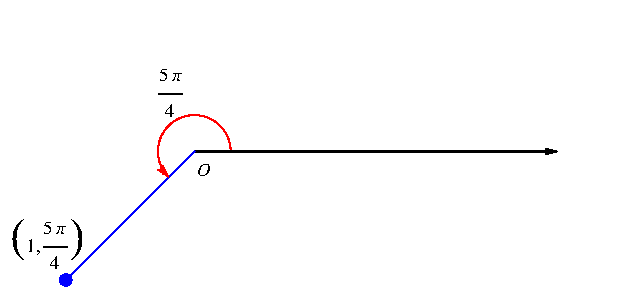
\includegraphics[height=3cm]{polar-curves/pictures/11-03-ex1a.pdf}%
%}%

%\ \uncover<2->{%
%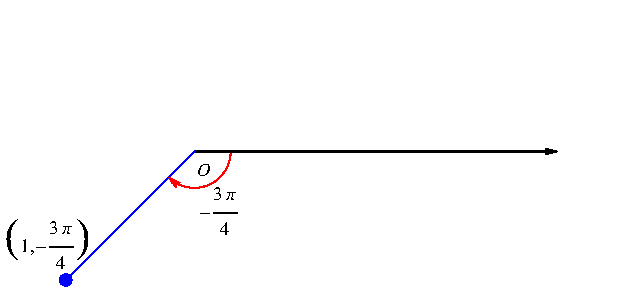
\includegraphics[height=3cm]{polar-curves/pictures/11-03-ex1b.pdf}%
%}%
\column{.5\textwidth}
\uncover<3->{
\psset{xunit=2cm, yunit=2cm}
\begin{pspicture}(-0.9, -1.1)(2,0.5)
\tiny
%force a boudning box:
%\psline[linecolor=red!1](-0.1, -0.1)(-0.21,0.2)
%\psline[linecolor=red!1](1.1, 0.6)(1.1,0.61)
\fcFullDotBlue{0}{0}

%Calculator input: plotCurve{}(1/50 t \cos{}t+3/20 \cos{}t, 1/50 t \sin{}t+3/20 \sin{}t, 0, 13/4 \pi)
\parametricplot[arrows=->, linecolor=\fcColorGraph, plotpoints=400] {0} {10.2102} {t 57.29578 mul cos 0.1500000 mul t 57.29578 mul cos t mul 0.0200000 mul add t 57.29578 mul sin 0.1500000 mul t 57.29578 mul sin t mul 0.0200000 mul add }

\rput[t] (0,-0.1){$O$}
\rput[l](0.3, 0.3){$\theta=\frac{13\pi}{4}$}

\psline{->}(0,0)(2,0)
\psline[linecolor=blue](0,0)(-0.707106781, -0.707106781)
\fcFullDotBlue{-0.707106781}{-0.707106781}
\rput[tl](-0.6, -0.7){$(r,\theta)=\left(1, \frac{13\pi}{4}\right)$}
\end{pspicture}
}

\uncover<4->{
\psset{xunit=2cm, yunit=2cm}
\begin{pspicture}(-0.9, -1.1)(2,0.5)
\tiny
%force a boudning box:
%\psline[linecolor=red!1](-0.1, -0.1)(-0.21,0.2)
\psline[linecolor=red!1](1.1, 0.5)(1.1,0.51)
\fcFullDotBlue{0}{0}

%Calculator input: plotCurve{}(1/10 \cos{}t, 1/10 \sin{}t, 0, -3/4 \pi)
\parametricplot[arrows=->, linecolor=\fcColorGraph, plotpoints=100]{0} {0.785398163} {t 57.29578 mul cos 0.3000000 mul t 57.29578 mul sin 0.3000000 mul }
\rput[t] (0,-0.1){$O$}
\rput[l](0.35, 0.15){$\theta=\frac{\pi}{4}$}

\psline{->}(0,0)(2,0)
\psline[linecolor=blue](0,0)(-0.707106781, -0.707106781)
\fcFullDotBlue{-0.707106781}{-0.707106781}
\psline[linestyle=dashed](0,0)(0.707106781, 0.707106781)
\fcFullDotBlack{0.707106781}{0.707106781}
\rput[tl](-0.6, -0.7){$(r,\theta)=\left(-1, \frac{\pi}{4}\right)$}
\end{pspicture}
}
%\ \uncover<3->{%
%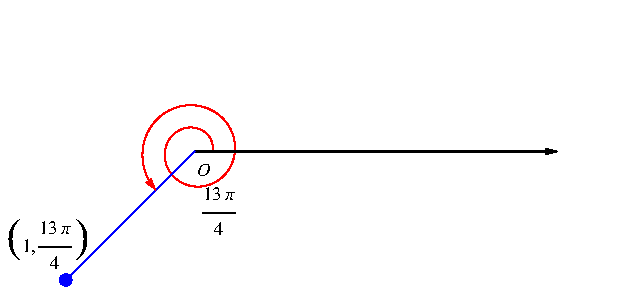
\includegraphics[height=3cm]{polar-curves/pictures/11-03-ex1c.pdf}%
%}%

%\ \uncover<4->{%
%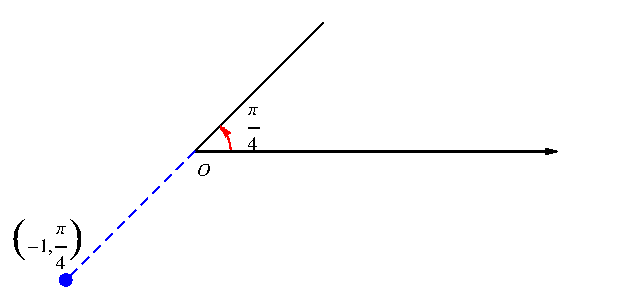
\includegraphics[height=3cm]{polar-curves/pictures/11-03-ex1d.pdf}%
%}%
\end{columns}
\begin{itemize}
\item  There are many ways to represent the same point.
\item<2-| alert@2>  We could use a negative $\theta$.
\item<3-| alert@3>  We could go around more than once.
\item<4-| alert@4>  We could use a negative $r$.
\end{itemize}
\end{frame}
% end module polar-many-representations

%begin module polar-two-points-coincide-iff
\begin{frame}
\begin{itemize}
\item Let $P_1$ be point  with polar coordinates $(r_1, \theta_1)$.
\item Let $P_2$ be point  with polar coordinates $(r_2, \theta_2)$.
\end{itemize}

\uncover<2->{
\begin{observation}
$P_1$ coincides with $P_2$ if one of the three mutually exclusive possibilities holds:
\begin{itemize}
\item<alert@3> $r_1=r_2\neq 0$ and $\theta_2=\theta_1+2k\pi, k\in \mathbb Z $,
\item<alert@4> $r_1=-r_2\neq 0$ and $\theta_2=\theta_1+(2k+1)\pi, k\in \mathbb Z$,
\item $r_1=r_2=0 $ and $\theta$ is arbitrary.
\end{itemize}
\end{observation}
}
\begin{columns}
\column{.5\textwidth}
\only<3>{
\psset{xunit=2cm, yunit=2cm}
\begin{pspicture}(-0.9, -1.1)(2,0.75)
\tiny
%force a boudning box:
%\psline[linecolor=red!1](-0.1, -0.1)(-0.21,0.2)
%\psline[linecolor=red!1](1.1, 0.6)(1.1,0.61)
\fcFullDotBlue{0}{0}

%Calculator input: plotCurve{}(1/10 \cos{}t, 1/10 \sin{}t, 0, -3/4 \pi)
\parametricplot[arrows=->, linecolor=\fcColorGraph, plotpoints=100]{0} {3.926990817} {t 57.29578 mul cos 0.3000000 mul t 57.29578 mul sin 0.3000000 mul }
\rput[t] (0,-0.1){$O$}
\rput[l](0.3, 0.3){$\theta_1$}

\psline{->}(0,0)(2,0)
\psline[linecolor=blue](0,0)(-0.707106781, -0.707106781)
\fcFullDotBlue{-0.707106781}{-0.707106781}
\rput[tl](-0.6, -0.7){$(r_1,\theta_1)$}
\end{pspicture}
}
\uncover<4>{
\psset{xunit=2cm, yunit=2cm}
\begin{pspicture}(-0.9, -1.1)(2,0.75)
\tiny
%force a boudning box:
%\psline[linecolor=red!1](-0.1, -0.1)(-0.21,0.2)
\psline[linecolor=red!1](1.1, 0.5)(1.1,0.51)
\fcFullDotBlue{0}{0}

%Calculator input: plotCurve{}(1/10 \cos{}t, 1/10 \sin{}t, 0, -3/4 \pi)
\parametricplot[arrows=->, linecolor=\fcColorGraph, plotpoints=100]{0} {-2.35619} {t 57.29578 mul cos 0.3000000 mul t 57.29578 mul sin 0.3000000 mul }
\rput[t] (0,-0.1){$O$}
\rput[l](0.3, -0.2){$\theta_1$}

\psline{->}(0,0)(2,0)
\psline[linecolor=blue](0,0)(-0.707106781, -0.707106781)
\fcFullDotBlue{-0.707106781}{-0.707106781}
\rput[tl](-0.6, -0.7){$(r_1,\theta_1)$}
\end{pspicture}
}

%\ \uncover<1->{%
%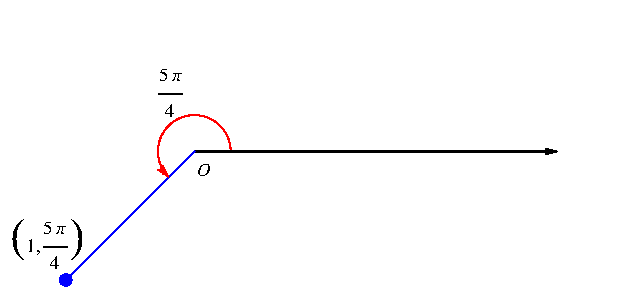
\includegraphics[height=3cm]{polar-curves/pictures/11-03-ex1a.pdf}%
%}%

%\ \uncover<2->{%
%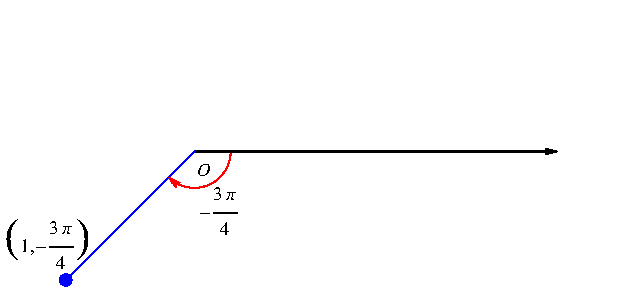
\includegraphics[height=3cm]{polar-curves/pictures/11-03-ex1b.pdf}%
%}%

\vspace{2cm}
\column{.5\textwidth}
\only<3>{
\psset{xunit=2cm, yunit=2cm}
\begin{pspicture}(-0.9, -1.1)(2,0.75)
\tiny
%force a boudning box:
%\psline[linecolor=red!1](-0.1, -0.1)(-0.21,0.2)
%\psline[linecolor=red!1](1.1, 0.6)(1.1,0.61)
\fcFullDotBlue{0}{0}

%Calculator input: plotCurve{}(1/50 t \cos{}t+3/20 \cos{}t, 1/50 t \sin{}t+3/20 \sin{}t, 0, 13/4 \pi)
\parametricplot[arrows=->, linecolor=\fcColorGraph, plotpoints=400] {0} {10.2102} {t 57.29578 mul cos 0.1500000 mul t 57.29578 mul cos t mul 0.0200000 mul add t 57.29578 mul sin 0.1500000 mul t 57.29578 mul sin t mul 0.0200000 mul add }

\rput[t] (0,-0.1){$O$}
\rput[l](0.3, 0.3){$\theta_2=\theta_1+2\pi$}

\psline{->}(0,0)(2,0)
\psline[linecolor=blue](0,0)(-0.707106781, -0.707106781)
\fcFullDotBlue{-0.707106781}{-0.707106781}
\rput[tl](-0.6, -0.7){$(r_2, \theta_2)=(r_1,\theta_1+2\pi)$}
\end{pspicture}
}

\uncover<4>{
\psset{xunit=2cm, yunit=2cm}
\begin{pspicture}(-0.9, -1.1)(2,0.75)
\tiny
%force a boudning box:
%\psline[linecolor=red!1](-0.1, -0.1)(-0.21,0.2)
\psline[linecolor=red!1](1.1, 0.5)(1.1,0.51)
\fcFullDotBlue{0}{0}

%Calculator input: plotCurve{}(1/10 \cos{}t, 1/10 \sin{}t, 0, -3/4 \pi)
\parametricplot[arrows=->, linecolor=\fcColorGraph, plotpoints=100]{0} {0.785398163} {t 57.29578 mul cos 0.3000000 mul t 57.29578 mul sin 0.3000000 mul }
\rput[t] (0,-0.1){$O$}
\rput[l](0.35, 0.15){$\theta_2=\theta_1+\pi$}

\psline{->}(0,0)(2,0)
\psline[linecolor=blue](0,0)(-0.707106781, -0.707106781)
\fcFullDotBlue{-0.707106781}{-0.707106781}
\psline[linestyle=dashed](0,0)(0.707106781, 0.707106781)
\fcFullDotBlack{0.707106781}{0.707106781}
\rput[tl](-0.6, -0.7){$(r_2, \theta_2)=(-r_1,\theta_1+\pi)$}
\end{pspicture}
}
%\ \uncover<3->{%
%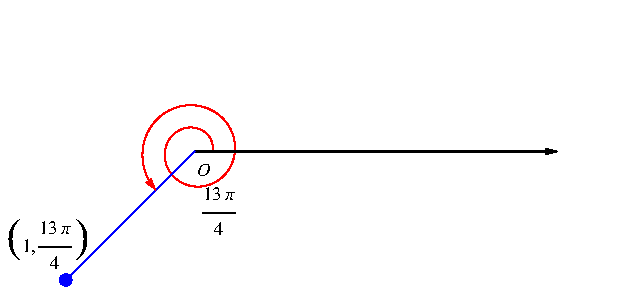
\includegraphics[height=3cm]{polar-curves/pictures/11-03-ex1c.pdf}%
%}%

%\ \uncover<4->{%
%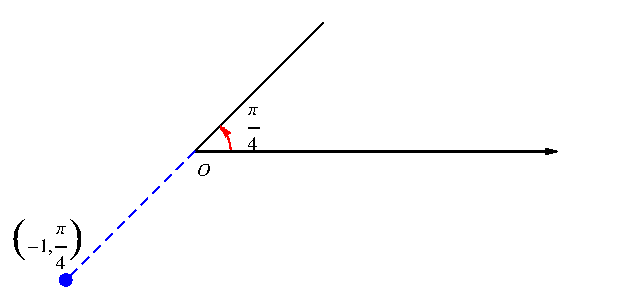
\includegraphics[height=3cm]{polar-curves/pictures/11-03-ex1d.pdf}%
%}%

\vspace{2cm}
\end{columns}
\end{frame}
%end module polar-two-points-coincide-iff

% begin module polar-to-cartesian
\begin{frame}
\begin{itemize}
\item  How do we go from polar coordinates to Cartesian coordinates?
\item<2->  Suppose a point has polar coordinates $(r, \theta )$ and Cartesian coordinates $(x,y)$.
\item<8->  How do we go from Cartesian coordinates to polar coordinates?
\end{itemize}
\begin{columns}[c]
\column{0.5\textwidth}
\psset{xunit=4cm, yunit=4cm}
\begin{pspicture}(-0.2, -0.2)(1.400000,0.9)
\tiny
%force a boudning box:
\psline[linecolor=red!1](-0.1, -0.1)(-0.21,0.2)
\psline[linecolor=red!1](1.1, 0.6)(1.1,0.61)
\psaxes[arrows=<->, ticks=none, labels=none](0,0)(-0.2, -0.2)(1, 0.8)
\rput(-0.03, 0.8){$y$}
\rput(1,-0.03){$x$}
%\fcAxesStandard{-0.2}{-0.2}{1}{0.8}

%Calculator input: plotCurve{}(1/5 \cos{}t, 1/5 \sin{}t, 0, 1/6 \pi)
\parametricplot[arrows=->, linecolor=red, plotpoints=1000] {0}{0.523599}{t 57.29578 mul cos 0.2 mul t 57.29578 mul sin 0.2 mul }
\psline[linecolor=blue](0,0)(0.866025404, 0.5)
\rput(0.22, 0.06){$\theta$}

\fcFullDotBlue{0.866025404}{0.5}
\psline(0.866025404,0.5)(0.866025404,0)
\psline(0.846025404, 0)(0.846025404, 0.02)(0.866025404, 0.02)
\rput[l](0.9, 0.5){$P(r,\theta) =(x,y)$}

\uncover<6>{
\psline{<-}(0.89, 0)(0.89, 0.2)
}
\uncover<6->{
\rput(0.89,0.25){$\alertNoH{6,10}{y}$}
}
\uncover<6>{
\psline{->}(0.89, 0.3)(0.89, 0.5)
}
\uncover<4>{
\psline{<-}(0, -0.02)(0.385, -0.02)
}
\uncover<4->{
\rput(0.435,-0.02){$\alertNoH{4,10}{x}$}
}
\uncover<4>{
\psline{->}(0.485, -0.02)(0.866025404, -0.02)
}
\rput[tr](-0.03, -0.03){$O$}
\rput(0.4, 0.3){$\alertNoH{4,6,9,10}{r}$}
\end{pspicture}
%\ \uncover<2->{%
%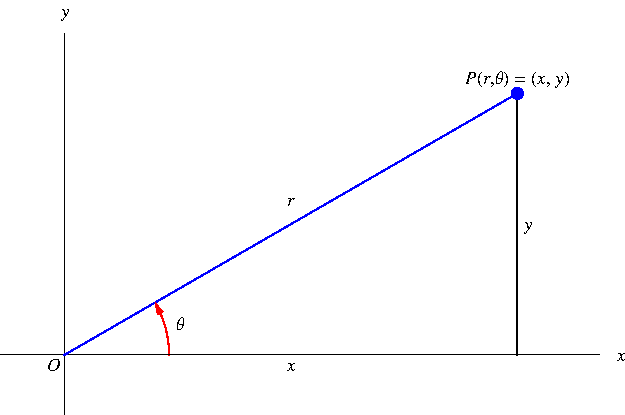
\includegraphics[height=5cm]{polar-curves/pictures/11-03-conversion.pdf}%
%}%
\column{.5\textwidth}
$
\renewcommand{\arraystretch}{1.5}
\begin{array}{rcl}
\alertNoH{7}{x} &\alertNoH{7}{=}&\uncover<7->{\alertNoH{7}{r\cos \theta} } \\
\alertNoH{7}{y}&\alertNoH{7}{=}& \uncover<7->{\alertNoH{7}{r\sin \theta}} \\\hline
\uncover<3->{\alertNoH{3,4,7}{\cos\theta}} & \uncover<3->{\alertNoH{3,4,7}{=}} &\displaystyle \uncover<4->{\alertNoH{4,7}{\frac{x}{r} }} \\
\uncover<3->{\alertNoH{5,6,7}{\sin \theta}} &\uncover<3->{ \alertNoH{5,6,7}{= }} & \displaystyle \uncover<6->{\alertNoH{6,7}{\frac{y}{r}}}\\
\uncover<9->{\alert<handout:0| 9-10>{r^2} &\alertNoH{9,10}{=}& \uncover<10->{\alertNoH{10}{x^2 + y^2}}}\\\hline
\alertNoH{8,9,10,11}{ r}&\alertNoH{8,9,10,11}{=}&\uncover<11->{\alertNoH{11}{ \sqrt{x^2+y^2}}} \\
\alertNoH{12,13}{\theta} &\alertNoH{12,13}{=}&
\uncover<13->{\alertNoH{13}{\arcsin \left(\frac{y}{r}\right)  \text{\quad if } x>0}}\\
\uncover<13->{
&\alertNoH{13}{=}&\alertNoH{13}{\arccos \left(\frac{x}{r}\right)  \text{\quad if } y>0}}\\
\uncover<13->{&\alertNoH{13}{=}&\alertNoH{13}{\arctan \left(\frac{y}{x}\right)  \text{\quad if } x>0}}
\end{array}
$


\end{columns}
\end{frame}
% end module polar-to-cartesian

% begin module polar-to-cartesian-ex2
\begin{frame}
\begin{example} %[Example 2, p. 677]
Convert the point $(\alert<handout:0| 4>{2}, \alert<handout:0| 6>{\pi/3})$ from polar to Cartesian coordinates.
\[
\uncover<2->{%
x = \alert<handout:0| 3-4>{r}\cos \alert<handout:0| 5-6>{\theta} = %
}%
\uncover<3->{%
\alert<handout:0| 3-4>{\uncover<4->{2}}\alert<handout:0| 7-8>{\cos} \alert<handout:0| 5-8>{\uncover<6->{\frac{\pi}{3}}} %
}%
\uncover<7->{%
 = 2\left( \alert<handout:0| 7-8>{\uncover<8->{\frac{1}{2}}}\right) \uncover<9->{ = 1}%
}%
\]
\[
\uncover<2->{%
y = r\sin \theta = %
}%
\uncover<10->{%
2\alert<handout:0| 11-12>{\sin \frac{\pi}{3}}%
}%
\uncover<11->{%
 = 2\left( \alert<handout:0| 11-12>{\uncover<12->{\frac{\sqrt{3}}{2}}}\right) \uncover<13->{ = \sqrt{3}}%
}%
\]
\uncover<14->{%
Therefore the point with polar coordinates $(2,\pi /3)$ has Cartesian coordinates $(1,\sqrt{3})$.
}%
\end{example}
\end{frame}
% end module polar-to-cartesian-ex2

% begin module polar-to-cartesian-ex3
\begin{frame}
\begin{example}
\begin{columns}
\column{0.25\textwidth}
\psset{xunit=0.65cm, yunit=0.65cm}
\begin{pspicture}(-1.5,-1.5)(1.6,1.6)
\tiny
\fcAxesStandard{-1.5}{-1.5}{1.6}{1.6}
\fcLabels{1.5}{1.5}
\uncover<9->{%
\fcFullDot{1}{-1}%
}%
\uncover<11->{% 
\fcAngleDegrees[arrows=->, linecolor=red]{0}{315}{0.2} { }%
\rput[b](-0.3, 0.2){$\frac{7\pi}{4}$}
\psline(0,0)(1,-1)
}%
\uncover<13->{%
\fcAngleDegrees{0}{-45}{0.4}{}
\rput[t](0.6, -0.2){$-\frac{\pi}{4}$}
}%
\end{pspicture}
\column{0.75\textwidth}
Represent the point with Cartesian coordinates $(1,-1)$ in terms of polar coordinates.
\end{columns}
\begin{columns}
\column{.6\textwidth}
\begin{itemize}
\item<3-| alert@3-4>  Suppose $r$ is positive.
\item<7->  $\tan \theta = -1$ for $\theta = \alert<handout:0| 10>{\frac{3\pi}{4}}, \alert<handout:0| 10-11>{\frac{7\pi}{4}}$, and many other angles.
\item<8-| alert@8-9>  $(1,-1)$ is in the \uncover<9->{fourth} quadrant.
\item<10->  Of the two values above, only \alert<handout:0| 10-11>{$\theta = \uncover<11->{\frac{7\pi}{4}}$} gives a point in the fourth quadrant.
\item<12->  $\Rightarrow$ one representation of $(1,-1)$ in polar coordinates is $\left(\sqrt{2}, \frac{7\pi}{4}\right)$.
\item<13->  $\left(\sqrt{2}, -\frac{\pi}{4}\right)$ is another.
\end{itemize}
\column{.4\textwidth}
\begin{eqnarray*}
\uncover<2->{%
r%
}%
& \uncover<2->{ = } &%
\uncover<2->{%
\uncover<-3>{\alert<handout:0| 3>{\pm}} \sqrt{x^2+y^2}%
}\\%
& \uncover<5->{ = } &%
\uncover<5->{%
\sqrt{1^2 + (-1)^2}%
}\\% = \sqrt{2}%
& \uncover<5->{ = } &%
\uncover<5->{%
\sqrt{2}%
}\\% = \sqrt{2}%
&&\\
\uncover<2->{%
\tan \theta%
}%
& \uncover<2->{ = } &%
\uncover<2->{%
\frac{y}{x}%
}\\%
& \uncover<6->{ = } &%
\uncover<6->{%
-1%
}\\%
\end{eqnarray*}
\end{columns}
\end{example}
\end{frame}
% end module polar-to-cartesian-ex3

%% begin module polar-intersection-ex3
\begin{frame}
\begin{example} %[Example 3, p. 688]
Find all points of intersection of the polar curves $r = \frac{1}{2}$ and $r = \cos (2\theta)$.
\begin{columns}[c]
\column{.4\textwidth}

\psset{xunit=1.8cm, yunit=1.8cm}
\begin{pspicture}(-1.5, -1.5)(1.5,1.5)
\tiny
\fcAxesStandard{-1.4}{-1.4}{1.4}{1.4}
%Calculator command: drawPolar{}(1/2, 0, 2 \pi)
\parametricplot[linecolor=\fcColorGraph, plotpoints=1000, algebraic=false]{0}{6.28319}{ 0.5 t 57.29578 mul cos mul 0.5 t 57.29578 mul sin mul }
%Calculator command: drawPolar{}(\cos{}(2 t), 0, 2 \pi)
\parametricplot[linecolor=\fcColorGraph, plotpoints=1000, algebraic=false]{0}{6.28319}{t 2 mul 57.29578 mul cos t 57.29578 mul cos mul t 2 mul 57.29578 mul cos t 57.29578 mul sin mul }

\rput[tr](-0.8, -0.8){$r=\frac{1}{2}$}
\psline{->}(-0.75, -0.75)(-0.353553391, -0.353553391)
\rput[lt] (0.2, -1){$r=\cos (2\theta)$}

\uncover<4->{
\fcFullDotBlack{0.433013}{0.25}
\fcFullDotBlack{-0.433013}{0.25}
\fcFullDotBlack{-0.433013}{-0.25}
\fcFullDotBlack{0.433013}{-0.25}
}
\uncover<6->{
\fcFullDotBlack{0.25}{0.433013}
\fcFullDotBlack{0.25}{-0.433013}
\fcFullDotBlack{-0.25}{-0.433013}
\fcFullDotBlack{-0.25}{0.433013}
}
\uncover<9>{
\pscircle*[linecolor=red](0.433013,0.25){0.09}
\pscircle*[linecolor=red](-0.433013,0.25){0.09}
\pscircle*[linecolor=red](-0.433013,-0.25){0.09}
\pscircle*[linecolor=red](0.433013,-0.25){0.09}
}
\uncover<10>{
\pscircle*[linecolor=red](0.25,0.433013){0.09}
\pscircle*[linecolor=red](0.25,-0.433013){0.09}
\pscircle*[linecolor=red](-0.25,-0.433013){0.09}
\pscircle*[linecolor=red](-0.25,0.433013){0.09}
}
\end{pspicture}

%\ \only<handout:0| -3>{%
%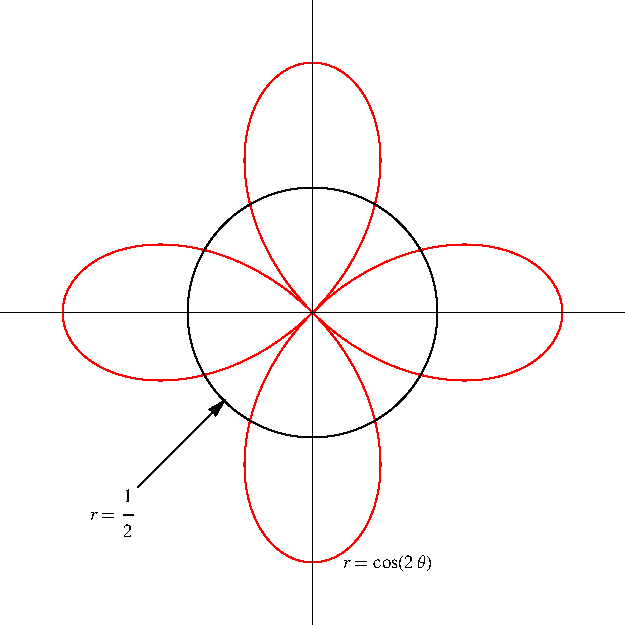
\includegraphics[height=5cm]{polar-curves/pictures/11-04-ex3a.pdf}%
%}%
%\only<handout:0| 4-5>{%
%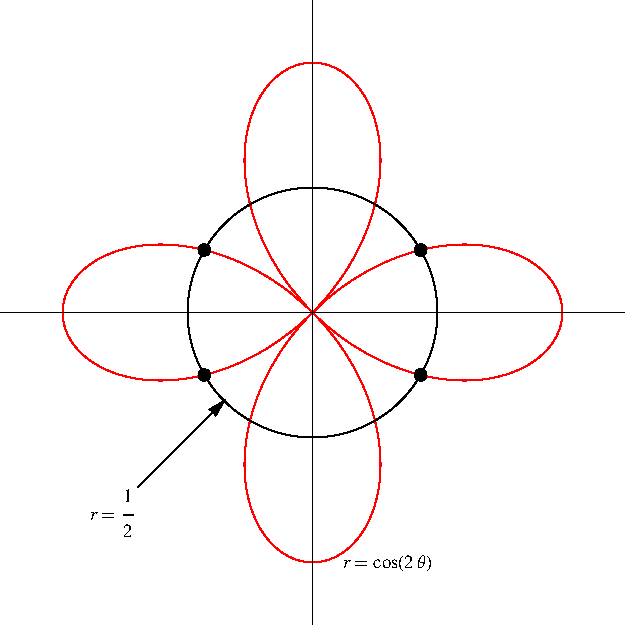
\includegraphics[height=5cm]{polar-curves/pictures/11-04-ex3b.pdf}%
%}%
%\only<6-8>{%
%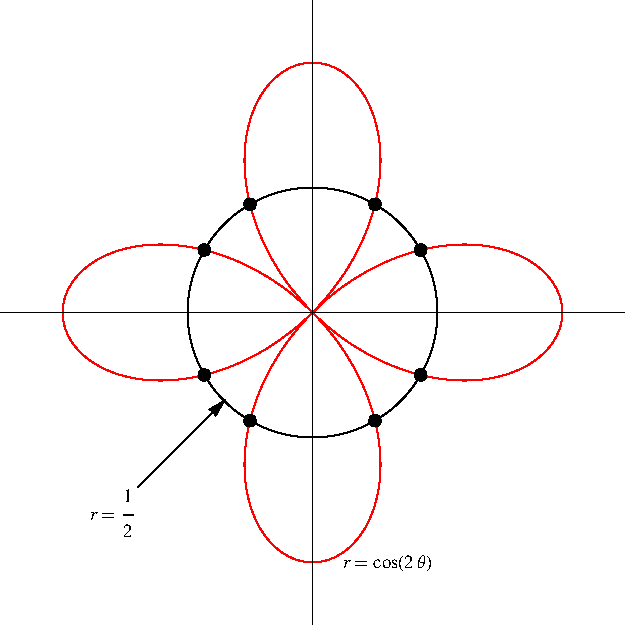
\includegraphics[height=5cm]{polar-curves/pictures/11-04-ex3c.pdf}%
%}%
%\only<handout:0| 9>{%
%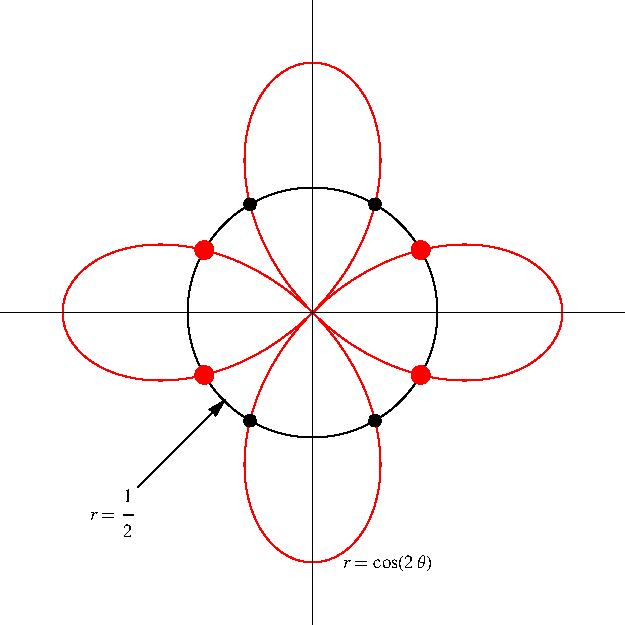
\includegraphics[height=5cm]{polar-curves/pictures/11-04-ex3d.pdf}%
%}%
%\only<handout:0| 10->{%
%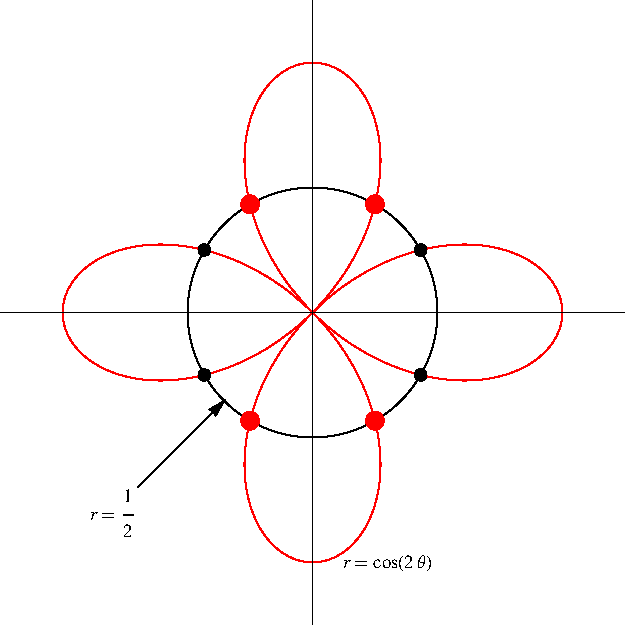
\includegraphics[height=5cm]{polar-curves/pictures/11-04-ex3e.pdf}%
%}%
\column{.6\textwidth}
\abovedisplayskip=0pt
\belowdisplayskip=0pt
\begin{eqnarray*}
\uncover<2->{%
\cos 2\theta%
}%
& \uncover<2->{ = } &%
\uncover<2->{%
\frac{1}{2}%
}\\%
\uncover<3->{%
2\theta%
}%
& \uncover<3->{ = } &%
\uncover<3->{%
\frac{\pi}{3}, \frac{5\pi}{3}, \frac{7\pi}{3}, \frac{11\pi}{3}%
}\\%
\uncover<4->{%
\theta%
}%
& \uncover<4->{ = } &%
\uncover<4->{%
\frac{\pi}{6}, \frac{5\pi}{6}, \frac{7\pi}{6}, \frac{11\pi}{6}%
}%
\end{eqnarray*}
\begin{itemize}
\item<5->  This only gives four points.
\item<6->  There are actually eight.
\item<7->  The circle $r = \frac{1}{2}$ also has polar equation $r = -\frac{1}{2}$.
\item<8->  To find all eight points, solve \alert<handout:0| 9>{$\cos (2\theta )= \frac{1}{2}$} and \alert<handout:0| 10>{$\cos (2\theta) = -\frac{1}{2}$}.
\end{itemize}
\end{columns}
\end{example}
\end{frame}
% end module polar-intersection-ex3


\section{Cylindrical Coordinates}
\begin{frame}
 \frametitle{Cylindrical coordinates}
\begin{columns}
\column{0.4\textwidth}
\psset{xunit=2.5cm, yunit=2.5cm}
\begin{pspicture}(-1, -1)(2,2)
\tiny
\renewcommand{\fcScreen}{[-3 -1 -1] 0}
\fcAxesIIId{1.5}{1.5}{1.5}
\fcLineIIId{[0 0 0]}{[1 1 1]}%
\fcPerpendicularIIId[linestyle=dashed]{[1 1 1]}{[0 0 1]}{0.2}%
\fcPerpendicularIIId{[1 1 1]}{[1 1 0]}{0.2}%
\fcPutIIId[bl]{[1 1 1]}{$~~P(x_P, y_P, z_P)$}
\fcPutIIId[tl]{[1 1 0]}{$~~\alert<6>{Q}$}
\fcPerpendicularIIId[linestyle=dashed]{[1 1 0]}{[1 0 0]}{0.2}%
\fcPerpendicularIIId[linestyle=dashed]{[1 1 0]}{[0 1 0]}{0.2}%
\fcLineIIId{[0 0 0]}{[1 1 0]}
\fcPutIIId[r]{[0.5 0 0]}{$x_P~~$}
\fcPutIIId[b]{[0 0.5 0]}{$y_P$}
\fcPutIIId[r]{[0 0 0.5]}{$\alert<5>{z_P~~}$}
\uncover<5>{%
\fcLineIIId[linecolor=red, linewidth=2pt]{[0 0 0]}{[0 0 1]}%
\fcLineIIId[linecolor=red, linewidth=2pt]{[1 1 1]}{[1 1 0]}%
}%
\fcDotIIId{[1 1 1]}%
\fcDotIIId{[1 1 0]}%
\fcPutIIId[tr]{[0.5 0.5 0]}{$\alert<6>{r_P}$}%
\fcAngleIIId[arrows=->, linecolor=red]{[1 0 0]}{[1 1 0]}{0.3}%
\uncover<7>{\fcAngleIIId[arrows=->, linecolor=red, linewidth=2pt]{[1 0 0]}{[1 1 0]}{0.3}}%
\uncover<6>{\fcLineIIId[linecolor=red, linewidth=2pt]{[0 0 0]}{[1 1 0]}}%
\fcPutIIId[t]{[0.4 0.2 0]}{$\alert<7>{\theta_P}$}
\end{pspicture}


\column{0.6\textwidth}

\begin{itemize}
\item In Cartesian $(x,y,z)$-coordinates, a point $P$ is given by triple $(x_P, y_P, z_P)$.
\item<2-> We introduce alternative cylindrical coordinates $(r_P, \theta_P ,z_P)$.
\item<3-> Cylindrical coordinates are obtained by ``adding a $z$-coordinate'' to the ($2$-dimensional) polar coordinates.
\item<4-> More precisely, to $P$ we assign triple $(\alert<5>{r_P}, \alert<6>{\theta_P}, \alert<7>{z_P})$, where:
\begin{itemize}
\item<5-> $\alert<5>{z_P}$ equals the $z$-coordinate of $P$,
\item<6-> $\alert<6>{r_P}$ is the distance $|OQ|$, where $Q$ is the projection of $P$ in the $xy$-plane and $O$-origin,
\item<7-> $\alert<7>{\theta_P}$ is an angle between the $x$-axis and $\fcv {OQ} $.
\end{itemize}
\end{itemize}
\end{columns}

\end{frame}

\begin{frame}
\frametitle{Cylindrical to and from cartesian coordinates}
\begin{columns}
\column{0.4\textwidth}
\psset{xunit=2.5cm, yunit=2.5cm}
\begin{pspicture}(-0.5, -1)(2,2)
\tiny
\renewcommand{\fcScreen}{[-3 -1 -1] 0}
\fcLineIIId[arrows=->]{[0 0 0]}{[1.5 0 0]}
\fcLineIIId[arrows=->]{[0 0 0]}{[0 1.5 0]}
\fcLineIIId[arrows=->]{[0 0 0]}{[0 0 1.5]}
\fcLineIIId{[0 0 0]}{[1 1 1]}%
\fcPerpendicularIIId[linestyle=dashed]{[1 1 1]}{[0 0 1]}{0.2}%
\fcPerpendicularIIId{[1 1 1]}{[1 1 0]}{0.2}%
\fcPutIIId[bl]{[1 1 1]}{$~~P(x, y, z)$}
\fcPutIIId[tl]{[1 1 0]}{$~~Q$}
\fcPerpendicularIIId[linestyle=dashed]{[1 1 0]}{[1 0 0]}{0.2}%
\fcPerpendicularIIId[linestyle=dashed]{[1 1 0]}{[0 1 0]}{0.2}%
\fcLineIIId{[0 0 0]}{[1 1 0]}
\fcPutIIId[r]{[0.5 0 0]}{$\alertNoH{2,3}{x}~~$}
\fcPutIIId[b]{[0 0.5 0]}{$\alertNoH{4,5}{y}$}
\fcPutIIId[r]{[0 0 0.5]}{$z~~$}
\fcDotIIId{[1 1 1]}
\fcDotIIId{[1 1 0]}
\fcPutIIId[tr]{[0.5 0.5 0]}{$\alertNoH{3,5}{r}~~$}
\fcAngleIIId[arrows=->, linecolor=red]{[1 0 0]}{[1 1 0]}{0.3}
\fcPutIIId[t]{[0.4 0.2 0]}{$\alertNoH{3,5}{\theta}$}
\uncover<3>{\fcAngleIIId[arrows=->, linecolor=red, linewidth=2pt]{[1 0 0]}{[1 1 0]}{0.3}}%
\uncover<3>{
\fcLineIIId[linewidth=2pt, linecolor=red]{[0 0 0]}{[1 0 0]}
}
\uncover<3,5>{
\fcLineIIId[linewidth=2pt, linecolor=red]{[0 0 0]}{[1 1 0]}
}
\uncover<5>{%
\fcLineIIId[linewidth=2pt, linecolor=red]{[1 0 0]}{[1 1 0]}%
\fcLineIIId[linewidth=2pt, linecolor=red]{[0 0 0]}{[0 1 0]}%
}%
\end{pspicture}
\column{0.6\textwidth}
To transform cylindrical to rectangular coordinates:
\uncover<2->{%
$$\begin{array}{rcl}
\alertNoH{2,3}{x}  &\alertNoH{2,3}{=}& \uncover<3->{\alertNoH{3}{ r \cos\theta }} \\
\alertNoH{4,5}{y} & \alertNoH{4,5}{=} &\uncover<5->{ \alertNoH{5}{ r \sin \theta}} \\
\alertNoH{6,7}{z_{rectangular}} &\alertNoH{6,7}{=}&\uncover<7->{ \alertNoH{7}{ z_{cylindrical}}}
\end{array}
$$
}

To transform rectangular to cylindrical:
$\begin{array}{rcl}
\renewcommand{\arraystretch}{1.7}
\alertNoH{8,9}{ r}&\alertNoH{8,9}{=}&\uncover<9->{\alertNoH{9}{ \sqrt{x^2+y^2}}} \\
\alertNoH{10,11}{\cos\theta} &\alertNoH{10,11}{=} &\displaystyle \uncover<11->{\alertNoH{11}{\frac{x}{r} }} \\
\alertNoH{10,11}{\sin \theta}&\alertNoH{10,11}{=}&\displaystyle \uncover<11->{\alertNoH{11}{\frac{y}{r}}}\\
\alertNoH{12,13}{\theta} &\alertNoH{12,13}{=}&
\uncover<13->{\alertNoH{13}{\arcsin \left(\frac{y}{r}\right)  \text{\quad if } x>0}}\\
\uncover<13->{
&\alertNoH{13}{=}&\alertNoH{13}{\arccos \left(\frac{x}{r}\right)  \text{\quad if } y>0}}\\
\uncover<13->{&\alertNoH{13}{=}&\alertNoH{13}{\arctan \left(\frac{y}{x}\right)  \text{\quad if } x>0}}\\
\alertNoH{14}{z_{cylindirical}}&\alertNoH{14}{=}&\uncover<14->{\alertNoH{14}{ z_{rectangular}}}
\end{array}
$

\end{columns}
\end{frame}



\begin{frame}
\frametitle{Constant Coordinate Sets}
\begin{columns}
\column{0.55\textwidth}
\psset{xunit=2.5cm, yunit=2.5cm}
\begin{pspicture}(-1, -1)(2,2)
\tiny%
\renewcommand{\fcScreen}{[-3 -1 -1] 0}%
\fcBoundingBox{-1.2}{-1.2}{2}{2}%
\fcLineIIId[arrows=->]{[0 0 0]}{[1.5 0 0]}%
\fcLineIIId[arrows=->]{[0 0 0]}{[0 1.5 0]}%
\fcLineIIId[arrows=->]{[0 0 0]}{[0 0 1.5]}%
\pstVerb{3 dict begin%
/xPoint 0.5 sqrt def%
/yPoint 0.5 sqrt def%
/zPoint 1 def%
}%
\multido{\na=1+1}{6}{\only<\na-7>{\pstVerb{%
/xPoint 1 \na\space 1 sub 10 div sub def%
/yPoint xPoint def%
}}%
\uncover<\na-6>{%
\fcDotIIId[linecolor=gray]{[1 \na\space 1 sub 10 div sub dup 1]}%
}%
}%
\multido{\na=8+1}{6}{\only<\na-14>{\pstVerb{%
\na\space 7 sub 12 mul dup
/xPoint exch cos def%
/yPoint exch sin def%
}}%
\uncover<\na-13>{%
\fcDotIIId[linecolor=gray]{[\na\space 7 sub 12 mul dup cos exch sin 1]}%
}%
}%
\multido{\na=15+1}{6}{\only<\na-21>{\pstVerb{%
/zPoint \na\space 15 sub -0.2 mul 1.2 add def%
}}%
\uncover<\na-20>{%
\fcDotIIId[linecolor=gray]{[xPoint yPoint \na\space 15 sub -0.2 mul 1.2 add]}%
}%
}%
\fcPerpendicularIIId[linestyle=dashed]{[xPoint yPoint zPoint]}{[0 0 1]}{0.2}%
\fcLineIIId{[0 0 0]}{[xPoint yPoint zPoint]}%
\fcPerpendicularIIId{[xPoint yPoint zPoint]}{[xPoint yPoint 0]}{0.2}%
\fcPutIIId[bl]{[xPoint yPoint zPoint]}{$~~P(x, y, z)$}
\fcPutIIId[tl]{[xPoint yPoint 0]}{$~~Q$}
\fcPerpendicularIIId[linestyle=dashed]{[xPoint yPoint 0]}{[1 0 0]}{0.2}%
\fcPerpendicularIIId[linestyle=dashed]{[xPoint yPoint 0]}{[0 1 0]}{0.2}%
\fcLineIIId{[0 0 0]}{[xPoint yPoint 0]}%
\fcPutIIId[r]{[xPoint 2 div 0 0]}{$x~~$}
\fcPutIIId[b]{[0 yPoint 2 div 0]}{$y$}
\fcPutIIId[r]{[0 0 zPoint 2 div]}{$z~~$}
\fcDotIIId{[xPoint yPoint zPoint]}%
\fcDotIIId{[xPoint yPoint 0]}%
\fcPutIIId[tr]{[xPoint 2 div yPoint 2 div 0]}{$r$}%
\fcAngleIIId[arrows=->, linecolor=red]{[1 0 0]}{[xPoint yPoint 0]}{0.3}%
\fcPutIIId[t]{[xPoint xPoint mul yPoint yPoint mul add sqrt dup xPoint exch div 0.4 mul exch yPoint exch div 2 div 0.4 mul 0]}{$\theta$}%
\uncover<7>{%
\fcLineIIId[arrows=->, linecolor=red]{[0 0 1]}{[1.4 1.4 1]}%
}%
\uncover<14>{%
\fcCurveIIId{-180}{180}{t cos t sin 1}%
}%
\uncover<21>{%
\fcLineIIId[linecolor=red]{[0.5 sqrt dup -0.2]}{[0.5 sqrt dup 1.5]}%
}%
\uncover<23>{%
\fcSurfaceIIId[linecolor=red]{iterationsX=11, iterationsY=11}{0}{-0.4}{180}{1}{u cos u sin  v}%
}%
\uncover<25>{%
\fcSurfaceIIId[linecolor=red]{iterationsX=11, iterationsY=17}{0}{-0.4}{1.6}{1.2}{u u v}%
}%
\uncover<27>{%
\fcSurfaceIIId[linecolor=red]{iterationsX=11, iterationsY=13}{0}{-180}{1.2}{180}{v sin u mul v cos u mul 1}%
}%
\pstVerb{end}%
\end{pspicture}
\column{0.45\textwidth}
What curve is traced when:
\begin{itemize}
\item \alert<1-7>{keep $\theta, z$ constant, let $r $ vary:} \uncover<7->{\alert<7>{horizontal ray;}}
\item \alert<8-14>{keep $r, z$ constant, let $\theta$ vary:} \uncover<14->{\alert<14>{horizontal circle;}}
\item \alert<15-21>{keep $r, \theta$ constant, let $z$ vary:} \uncover<21->{\alert<21>{ vertical line.}}
\end{itemize}

What surface is traced when:
\begin{itemize}
\item \alert<22,23>{keep $r$ constant, let $\theta, z$ vary:} \uncover<23->{\alert<23>{vertical cylinder;}}
\item \alert<24,25>{keep $\theta$ constant, let $r,z$ vary:} \uncover<25->{\alert<25>{vertical half plane;}}
\item \alert<26,27>{keep $z$ constant, let $r,\theta$ vary:} \uncover<27->{\alert<27>{horizontal plane.}}
\end{itemize}
\uncover<15>{}
\end{columns}
\end{frame}
\section{Spherical Coordinates}
\begin{frame}
 \frametitle{Spherical Coordinates}
\begin{columns}
\column{0.55\textwidth}
%  \psfrag{P}{$P$}
%  \psfrag{O}{$O$}  
%  \psfrag{xp}{$x_P$} 
%  \psfrag{yp}{$y_P$} 
%  \psfrag{zp}{$z_P$}     
%  \psfrag{rho}{$\rho_P$}
%  \psfrag{thp}{$\theta_P$}
%  \psfrag{phi}{$\phi_P$}
\psset{xunit=1cm, yunit=1cm}
\begin{pspicture}(-2,-2.5)(2,2)
\tiny
\renewcommand{\fcScreen}{[-1 -0.4 -0.25] -1}
\fcBoundingBox{-2}{-2.5}{2}{2}
\fcAxesIIId{5}{5}{5}
\fcPutIIId[r]{[0 -0.15 0.15]}{$O$}
\fcLineIIId[linestyle=dotted]{[3 0 0]}{[3 3 0]}
\fcLineIIId[linestyle=dotted]{[3 3 0]}{[0 3 0]}
\fcLineIIId[linestyle=dotted]{[0 0 0]}{[0 3 0]}
\fcLineIIId{[0 0 0]}{[3 3 0]}
\fcLineIIId{[3 3 0]}{[3 3 3]}
\fcLineIIId{[0 0 3]}{[3 3 3]}
\fcPutIIId[l]{[3.1 3.1 3.1]}{$P$}
\fcPutIIId[r]{[1.5 -0.1 0]}{$x_P$}
\fcPutIIId[t]{[3 3 0]}{$Q$}
\fcPutIIId[b]{[0 1.5 0]}{$y_P$}
\fcPutIIId[l]{[3 3 1.5]}{$~~z_P$}
\fcPutIIId[r]{[0 0 1.5]}{$z_P~~$}
\uncover<2->{%
\fcLineIIId{[0 0 0]}{[3 3 3]}
\uncover<3>{\fcLineIIId[linecolor=red, linewidth=2pt]{[0 0 0]}{[3 3 3]}}%
\fcPutIIId[r]{[2.1 2.1 2.1]}{$\rho_P$}
\fcPutIIId[rt]{[1 1 1.5]}{$\phi_P~~$}
\fcPutIIId[tr]{[1.8 0.9 0]}{$\theta_P$}%
\fcAngleIIId[linecolor=red, arrows=->]{[0 0 1]}{[3 3 3]}{1.7}%
\uncover<4>{\fcAngleIIId[linecolor=red, linewidth=2pt, arrows=->]{[0 0 1]}{[3 3 3]}{1.7}}%
\fcAngleIIId[linecolor=red, arrows=->]{[1 0 0]}{[3 3 0]}{1.7}%
\uncover<5>{\fcAngleIIId[linecolor=red, arrows=->, linewidth=2pt]{[1 0 0]}{[3 3 0]}{1.7}}%
}%
\uncover<8>{\fcLineIIId[arrows=->, linecolor=red, linewidth=2pt]{[0 0 0]}{[5 5 5]}}%
\uncover<10>{%
\fcAngleIIId[linecolor=red, linewidth=2pt]{[0 0 1]}{[1 1 0]}{2}%
\fcAngleIIId[linecolor=red, linewidth=2pt, arrows=->]{[1 1 0]}{[0 0 -1]}{2}%
}%
\uncover<12>{%
\fcAngleIIId[linecolor=red, linewidth=2pt]{[1 0 0]}{[0 1 0]}{2}%
\fcAngleIIId[linecolor=red, linewidth=2pt]{[0 1 0]}{[-1 0 0]}{2}%
\fcAngleIIId[linecolor=red, linewidth=2pt]{[-1 0 0]}{[0 -1 0]}{2}%
\fcAngleIIId[linecolor=red, linewidth=2pt, arrows=->]{[0 -1 0]}{[1 0 0]}{2}%
}%
\end{pspicture}   
%  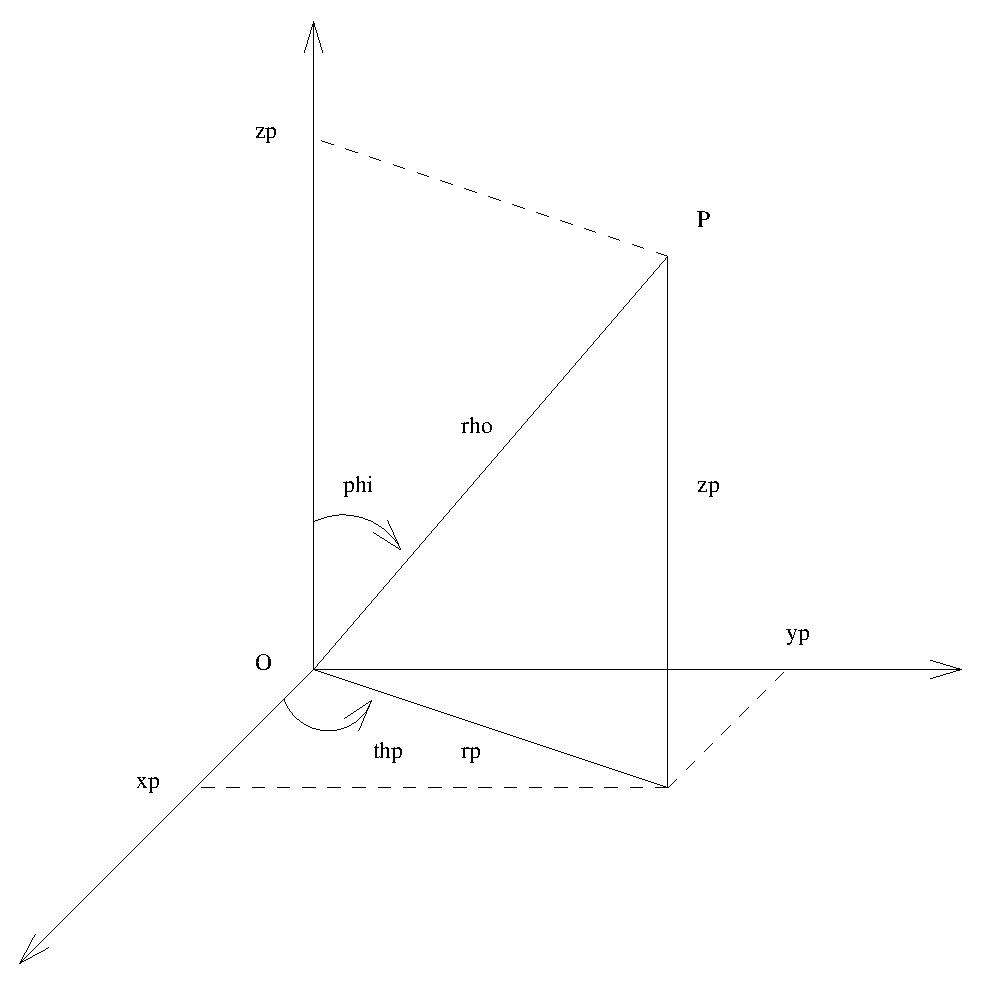
\includegraphics[height=2in]{../../modules/coordinate-systems/pictures/ok-cylindrical-spherical.eps}
\column{0.45\textwidth}
	\begin{itemize}
\item In Cartesian coordinates, a point $P$ is given by triple $(x_P, y_P, z_P)$.
\item<2-> We introduce alternative spherical coordinates $(\rho_P, \phi_P,\theta_P)$.
\begin{itemize}
\item \alert<3>{$\rho_P$: distance $|OP|$;}
\item \alert<4>{$\phi_P$: angle $Oz$ to $OP$;}
\item \alert<5>{$\theta_P$: angle $Ox$ to $OP_{xy}$.}
\end{itemize}
\item<6-> Coordinates range:
\begin{itemize}
\item \alert<7,8>{$\rho$:} \uncover<8->{\alert<8>{ $[0,\infty)$;}}
\item \alert<9,10>{$\phi$:}  \uncover<10->{\alert<10>{$[0, \pi]$;}}
\item \alert<11,12>{$\theta$:}  \uncover<12->{ \alert<12>{$[0,2\pi)$.}}
\end{itemize}
\end{itemize}
\end{columns}
\end{frame}
\begin{frame}
\frametitle{Transition Spherical - Rectangular coordinates}
\begin{columns}
\column{0.4\textwidth}
\psset{xunit=1cm, yunit=1cm}
\begin{pspicture}(-3,-2)(2,2)
\tiny
\renewcommand{\fcScreen}{[-1 -0.4 -0.25] -1}
\fcLineIIId[arrows=->]{[0 0 0]}{[5 0 0 ]}
\fcLineIIId[arrows=->]{[0 0 0]}{[0 5 0 ]}
\fcLineIIId[arrows=->]{[0 0 0]}{[0 0 5 ]}
\fcPutIIId[r]{[0 -0.15 0.15]}{\alert<2,3,4>{$O$}}
\fcLineIIId[linecolor=gray]{[3 0 0]}{[3 3 0]}
\fcLineIIId[linecolor=gray]{[3 3 0]}{[0 3 0]}
\fcLineIIId{[0 0 0]}{[3 3 0]}
\fcLineIIId{[3 3 0]}{[3 3 3]}
\fcLineIIId{[0 0 0]}{[3 3 3]}
\fcLineIIId{[0 0 3]}{[3 3 3]}
\fcPutIIId[l]{[3.1 3.1 3.1]}{\alert<4>{$P$}}
\fcPutIIId[r]{[1.5 -0.1 0]}{$\alert<1>{x}$}
\fcPutIIId[t]{[3.1 3.1 0]}{\alert<2,3>{$Q$}}
\uncover<2->{\fcPutIIId[l]{[1.4 1.5 0]}{\alert<4,5,6>{$~~r$}}}
\uncover<2->{
\fcPutIIId[r]{[3 -0.1 0]}{\alert<2,3>{$S$}}
\fcPolyLineIIId[linecolor=red]{[2.6 0 0 ] [2.6 0.4 0] [3 0.4 0]}
}
\uncover<2->{
\fcPutIIId[b]{[-0.1 1.5 0]}{$y$}
\fcPutIIId[t]{[3.1 1.5 0]}{\alert<5>{$y$}}
}
\uncover<7->{\fcPutIIId[r]{[0 0 1.5]}{\alert<7>{$z~~$}}}
\uncover<4->{
\fcPutIIId[r]{[0 -0.1 3]}{\alert<4>{$T~$}}
\fcPutIIId[b]{[1.4 1.5 3]}{\alert<4,6>{$~~r$}}
\fcPolyLineIIId[linecolor=red]{[2.6 2.6 0] [2.6 2.6 0.56569] [3 3 0.56569]}
\fcPolyLineIIId[linecolor=red]{[0.4 0.4 3] [0.4 0.4 3 0.56569 sub] [0 0 3 0.56569 sub]}
}
\fcPutIIId[r]{[1.7 1.7 1.7]}{\alert<4,6,7>{$\rho~~$}}
\fcPutIIId[rt]{[0.8 0.8 1.3]}{\alert<4,6,7>{$\phi~~$}}
\fcPutIIId[br]{[1.2 0.5 0]}{\alert<3,5>{$\theta$}}
\fcCurveIIId[linecolor=red, arrows=->]{0}{54.74}{[t sin 45 cos mul 1.5 mul t sin 45 sin mul 1.5 mul t cos 1.5 mul ]} %
\fcCurveIIId[linecolor=red, arrows=->]{0}{45}{[t cos 1.5 mul t sin 1.5 mul 0]} %
\end{pspicture}
\column{0.6\textwidth}

From spherical to rectangular coords:
\[
\begin{array}{rcll|l}
\alert<1->{x}&\alert<1>{=}& \uncover<3->{\alert<3>{ \alert<4>{r}\cos\theta}} &&\uncover<2->{\alert<2,5>{ \text{use }\triangle SQO}} \\
\uncover<4->{&\alert<0>{=} & \alert<4>{\rho\sin\phi }\cos\theta &&\alert<4,6,7>{ \text{use }\triangle OPT} }\\
\uncover<5->{\alert<5>{y}&\alert<0>{=}& \alert<5>{\alert<6>{r} \sin\theta } }\\
\uncover<6->{&\alert<0>{=}& \alert<6>{\rho\sin\phi }\sin\theta} \\
\uncover<7->{\alert<7>{z}&\alert<7>{=}& \alert<7>{\rho\cos\phi }}
\end{array}
\]
\uncover<8->{
From rectangular to spherical coords:
$$\rho = \sqrt{x^2+y^2+z^2} \quad , \quad r = \sqrt{x^2+y^2}$$
$$\cos\phi = \frac{z}{\rho} \quad , \quad \sin\phi = \frac{r}{\rho}$$
$$\cos\theta = \frac{x}{r} \quad , \quad \sin\theta = \frac{y}{r}$$
}
\end{columns}
\end{frame}




\begin{frame}
\frametitle{Constant Coordinate Sets}
\begin{columns}
\column{0.55\textwidth}
\psset{xunit=1cm, yunit=1cm}
\begin{pspicture}(-1, -1)(2,2)
\tiny%
\fcBoundingBox{-3}{-3.3}{3}{3.8}%
\renewcommand{\fcScreen}{[-1 -0.4 -0.25] -1}
\fcLineIIId[arrows=->]{[0 0 0]}{[3.2 0 0 ]}
\uncover<13,14>{\fcLineIIId[arrows=->]{[0 0 0]}{[-3.2 0 0 ]}}
\uncover<18-21>{\fcLineIIId[arrows=->]{[0 0 0]}{[0 0 -3.2 ]}}
\fcLineIIId[arrows=->]{[0 0 0]}{[0 3.2 0 ]}
\fcLineIIId[arrows=->]{[0 0 0]}{[0 0 3.2 ]}
\pstVerb{4 dict begin%
/xPoint 8 3 div sqrt def%
/yPoint xPoint def%
/zPoint 4 3 div sqrt def%
/rho xPoint dup mul yPoint dup mul zPoint dup mul add add sqrt def%
}%
\multido{\na=1+1}{6}{\only<\na-7>{\pstVerb{%
/xPoint 3 \na\space 1 sub 3 div sub def%
/yPoint xPoint def%
/zPoint xPoint def%
/rho xPoint dup mul yPoint dup mul zPoint dup mul add add sqrt def%
}}%
\uncover<\na-6>{%
%\fcDotIIId[linecolor=gray]{[3 \na\space 1 sub 3 div sub dup dup]}%
\fcDotIIId[linecolor=gray]{[xPoint yPoint zPoint]}%
}%
}%
\multido{\na=8+1}{6}{\only<\na-14>{\pstVerb{%
/rho 3 def%
/zPoint 3 sqrt def %
\na\space 7 sub 20 mul dup%
/xPoint exch cos 6 sqrt mul def%
/yPoint exch sin 6 sqrt mul def%
}}%
\uncover<\na-13>{%
\fcDotIIId[linecolor=gray]{[xPoint yPoint zPoint]}%
}%
}%
\multido{\na=15+1}{6}{\only<\na-21>{\pstVerb{%
/rho 3 def %
\na\space 13 sub 20 mul dup%
/xPoint exch sin 0.5 sqrt mul rho mul def%
/yPoint xPoint def%
/zPoint exch cos rho mul def%
}}%
\uncover<\na-20>{%
\fcDotIIId[linecolor=gray]{[xPoint yPoint zPoint]}%
}%
}%
\fcPutIIId[r]{[0 -0.15 0.15]}{$O$}
\fcLineIIId{[0 0 0]}{[xPoint yPoint 0]}
\fcLineIIId{[0 0 0]}{[xPoint yPoint zPoint]}
\fcPutIIId[l]{[xPoint yPoint zPoint]}{$~~P$}
\fcPutIIId[r]{[xPoint 2 div -0.1 0]}{$x$}
\fcPutIIId[t]{[xPoint yPoint 0]}{$~~Q$}
\fcPutIIId[lb]{[xPoint 2 div yPoint 2 div 0]}{$~~r$}
\fcPerpendicularIIId[linecolor=gray]{[xPoint yPoint zPoint]}{[0 0 1]}{0.4}%
\fcPerpendicularIIId[linecolor=gray]{[xPoint yPoint zPoint]}{[xPoint yPoint 0]}{0.4}%
\fcPerpendicularIIId[linecolor=gray]{[xPoint yPoint 0]}{[1 0 0]}{0.4}%
\fcPerpendicularIIId[linecolor=gray]{[xPoint yPoint 0]}{[0 1 0]}{0.4}%
\fcDotIIId{[xPoint yPoint zPoint]}%
\fcPutIIId[b]{[-0.1 yPoint 2 div 0]}{$y$}
\fcPutIIId[r]{[0 0 zPoint 2 div]}{$z~~$}
\fcPutIIId[r]{[xPoint 2 div yPoint 2 div zPoint 2 div]}{$\rho~~$}
\fcAngleIIId[arrows=->, linecolor=red]{[0 0 1]}{[xPoint yPoint zPoint]}{0.7}%
\fcAngleIIId[arrows=->, linecolor=red]{[1 0 0]}{[xPoint yPoint 0]}{0.7}%
\fcPutIIId[lb]{[xPoint rho div 0.5 mul yPoint rho div 0.5 mul zPoint rho div 1.2 mul]}{$\phi~~$}
\fcPutIIId[t]{[xPoint rho div 1.5 mul yPoint rho div 0.7 mul 0]}{$\theta~~$}
\uncover<7>{\fcLineIIId[arrows=->, linecolor=red, linewidth=2pt]{[0 0 0]}{[4 4 4]}
}
\uncover<14>{%
\fcCurveIIId[arrows=->, linecolor=red, linewidth=2pt]{0}{360}{[t cos 6 sqrt mul t sin 6 sqrt mul zPoint]}%
}%
\uncover<21>{%
\fcCurveIIId[arrows=->, linecolor=red, linewidth=2pt]{0}{180}{[t sin rho mul 0.5 sqrt mul dup t cos rho mul]}%
}%
\uncover<23>{%
\fcSurfaceDirectDraw[linecolor=red]{iterationsX=11, iterationsY=17}{0}{0}{3 sqrt}{360}{[v cos u mul 8 3 div sqrt mul v sin u mul 8 3 div sqrt mul u 4 3 div sqrt mul]}%
}%
\uncover<25>{%
\fcSurfaceDirectDraw[linecolor=red]{iterationsX=11, iterationsY=17}{0}{0}{2}{180}{[v sin u mul 0.5 sqrt mul dup v cos u mul]}%
}%
\uncover<27>{%
\fcSurfaceDirectDraw[linecolor=red]{iterationsX=11, iterationsY=17}{0}{-90}{180}{90}{[u sin v cos 2 mul mul u sin v sin 2 mul mul u cos 2 mul]}%
}%
\pstVerb{end}%
\end{pspicture}
\column{0.45\textwidth}
\only<1-21>{
What curve is traced when:
\begin{itemize}
\item \alert<1-7>{keep $\theta, \phi$ constant, let $\rho$ vary:} \uncover<7->{\alert<7>{ray through the origin;}}
\item \alert<8-14>{keep $\rho, \phi$ constant, let $\theta$ vary:} \uncover<14->{\alert<14>{circle parallel to the $xy$-plane, ``parallel'';}}
\item \alert<15-21>{keep $\rho, \theta$ constant, let $\phi$ vary:} \uncover<21->{\alert<21>{circle passing through $z$ axis, ``meridian''.}}
\end{itemize}
}
\only<22->{
What surface is traced when:
\begin{itemize}
\item \alert<22,23>{keep $\phi$ constant, let $\theta, \rho$ vary:} \uncover<23->{\alert<23>{cone;}}
\item \alert<24,25>{keep $\theta$ constant, let $\rho,\phi$ vary:} \uncover<25->{\alert<25>{vertical half plane;}}
\item \alert<26,27>{keep $\rho$ constant, let $\phi,\theta$ vary:} \uncover<27->{\alert<27>{sphere.}}
\end{itemize}
}
\end{columns}
\end{frame}


\section{Curvilinear boxes}
\begin{frame}
 \frametitle{Polar curvilinear ``boxes''}

 Polar ``wedge'':
 %
$$C  = \{ P(r,\theta) \; | \;r_0 \leqslant
r \leqslant r_0+\Delta r,  \theta_0 \leqslant \theta
\leqslant \theta_0+\Delta \theta\} \; .$$
%
Shape? \pause Area = ...?

\end{frame}
\begin{frame}
 \frametitle{Cylindrical curvilinear ``boxes''}

Cylindrical ``box'':
%
$$X = \{ P(r,\theta, z) \; | \; 0 \leqslant r \leqslant r_0\, ,
0 \leqslant \theta \leqslant \theta_0\, ,
0 \leqslant z \leqslant z_0\}$$

\pause
Shape ? \pause Volume = ...?

\end{frame}
\begin{frame}
\frametitle{Spherical curvilinear ``boxes''}


\begin{columns}
\column{0.4\textwidth}

\psset{xunit=1.5cm, yunit=1.5cm}
\begin{pspicture}(-2, -2)(2,2)
\tiny
\renewcommand{\fcScreen}{[-5 1 -2.4] 0}
\pstVerb{10 dict begin%
/rhoMin 1 def%
/rhoMax 2 def%
/thetaMin 20 def%
/thetaMax 70 def%
/phiMin 20 def%
/phiMax 70 def%
/xSph {theta cos phi sin rho mul mul} def%
/ySph {theta sin phi sin rho mul mul} def%
/zSph {phi cos rho mul} def%
}%
\fcAxesIIId{2}{2}{2}
\uncover<10->{
\pscustom*[linecolor=pink]{%
\fcCurveIIId{phiMin}{phiMax}{ 3 dict begin /rho rhoMin def /phi t def /theta thetaMin def xSph ySph zSph end}
\fcCurveIIId{rhoMin}{rhoMax}{ 3 dict begin /rho t def /phi phiMax def /theta thetaMin def xSph ySph zSph end}
\fcCurveIIId{thetaMin}{thetaMax}{ 3 dict begin /rho rhoMax def /phi phiMax def /theta t def xSph ySph zSph end}
\fcCurveIIId{phiMax}{phiMin}{ 3 dict begin /rho rhoMax def /phi t def /theta thetaMax def xSph ySph zSph end}
\fcCurveIIId{thetaMax}{thetaMin}{ 3 dict begin /rho rhoMax def /phi phiMin def /theta t def xSph ySph zSph end}
\fcCurveIIId{rhoMax}{rhoMin}{ 3 dict begin /rho t def /phi phiMin def /theta thetaMin def xSph ySph zSph end}
}%
}%
\fcLineIIId[linestyle=dashed]{[0 0 0]}{[0 2 0]}

\uncover<7->{\fcCurveIIId{rhoMin}{rhoMax}{ 3 dict begin /rho t def /phi phiMin def /theta thetaMin def xSph ySph zSph end}}
\uncover<5->{\fcCurveIIId{rhoMin}{rhoMax}{ 3 dict begin /rho t def /phi phiMax def /theta thetaMin def xSph ySph zSph end}}
\uncover<9->{\fcCurveIIId[linestyle=dashed, linecolor=red]{rhoMin}{rhoMax}{ 3 dict begin /rho t def /phi phiMin def /theta thetaMax def xSph ySph zSph end}}
\uncover<9->{\fcCurveIIId[linestyle=dashed, linecolor=red]{rhoMin}{rhoMax}{ 3 dict begin /rho t def /phi phiMax def /theta thetaMax def xSph ySph zSph end}}

\uncover<8->{%
\fcCurveIIId[linestyle=dashed, dash = 2.6pt,  linecolor=red] {thetaMin}{thetaMax}{ 3 dict begin /rho rhoMin def /phi phiMin def /theta t def xSph ySph zSph end}
\fcCurveIIId{thetaMin}{thetaMax}{ 3 dict begin /rho rhoMax def /phi phiMin def /theta t def xSph ySph zSph end}
\fcCurveIIId[linestyle=dashed, linecolor=red]{thetaMin}{thetaMax}{ 3 dict begin /rho rhoMin def /phi phiMax def /theta t def xSph ySph zSph end}
\fcCurveIIId{thetaMin}{thetaMax}{ 3 dict begin /rho rhoMax def /phi phiMax def /theta t def xSph ySph zSph end}
}%

\uncover<4->{\fcCurveIIId{phiMin}{phiMax}{ 3 dict begin /rho rhoMin def /phi t def /theta thetaMin def xSph ySph zSph end}}
\uncover<9->{\fcCurveIIId[linestyle=dashed, linecolor=red]{phiMin}{phiMax}{ 3 dict begin /rho rhoMin def /phi t def /theta thetaMax def xSph ySph zSph end}}
\uncover<6->{\fcCurveIIId{phiMin}{phiMax}{ 3 dict begin /rho rhoMax def /phi t def /theta thetaMin def xSph ySph zSph end}}
\uncover<9->{\fcCurveIIId{phiMin}{phiMax}{ 3 dict begin /rho rhoMax def /phi t def /theta thetaMax def xSph ySph zSph end}}
\pstVerb{end}
\end{pspicture}

\psset{xunit=1cm, yunit=1cm}
\begin{pspicture}(-2, -2)(2,2)
\tiny
\pstVerb{10 dict begin%
/rhoMin 1 def%
/rhoMax 2 def%
/thetaMin 20 57.2957795 div def%
/thetaMax 70 57.2957795 div  def%
/phiMin 20 57.2957795 div def%
/phiMax 70 57.2957795 div def%
}%
\fcAxesIIId[arrows=->, xLabel=$~~\rho$, yLabel=$~~\phi$, zLabel=$~~\theta$]{2.5}{3.8}{2.5}
\pscustom*[linecolor=cyan]{%
\fcPolyLineIIId{[rhoMin phiMin thetaMin] [rhoMax phiMin thetaMin] [rhoMax phiMax thetaMin] [rhoMax phiMax thetaMax] [rhoMin phiMax thetaMax] [rhoMin phiMin thetaMax] [rhoMin phiMin thetaMin]}
}
\fcLineIIId[linestyle=dashed]{[0 0 0]}{[0 3.8 0]}
\fcDotIIId{[rhoMin 0 0 ]}
\fcPutIIId[t]{[rhoMin 0 -0.2 ]}{$\rho_{min}$}
\fcDotIIId{[rhoMax 0 0 ]}
\fcPutIIId[t]{[rhoMax 0 -0.2 ]}{$\rho_{max}$}
\fcDotIIId{[0 0 thetaMin  ]}
\fcPutIIId[r]{[0 0 thetaMin]}{$\theta_{min}~~$}
\fcDotIIId{[0 0 thetaMax]}
\fcPutIIId[r]{[0 0 thetaMax]}{$\theta_{max}~~$}
\fcDotIIId{[0  phiMin 0  ]}
\fcPutIIId[b]{[0 phiMin 0.2 ]}{$~\phi_{min}$}
\fcDotIIId{[0  phiMax 0  ]}
\fcPutIIId[b]{[0 phiMax 0.2 ]}{$\phi_{max}$}

\fcLineIIId[linecolor=blue, linestyle=dashed]{[rhoMin phiMax thetaMin]}{[rhoMax phiMax thetaMin]}
\uncover<5-9>{\fcLineIIId[linecolor=red, linewidth=2pt, linestyle=dashed]{[rhoMin phiMax thetaMin]}{[rhoMax phiMax thetaMin]}}
\fcLineIIId[linecolor=blue]{[rhoMax phiMax thetaMin]}{[rhoMax phiMin thetaMin]}
\uncover<6-9>{\fcLineIIId[linecolor=red, linewidth=2pt]{[rhoMax phiMax thetaMin]}{[rhoMax phiMin thetaMin]}
}
\fcLineIIId[linecolor=blue]{[rhoMax phiMin thetaMin]}{[rhoMin phiMin thetaMin]}
\uncover<7-9>{\fcLineIIId[linecolor=red, linewidth=2pt]{[rhoMax phiMin thetaMin]}{[rhoMin phiMin thetaMin]}}
\fcLineIIId[linecolor=blue, linestyle=dashed]{[rhoMin phiMin thetaMin]}{[rhoMin phiMax thetaMin]}
\uncover<4-9>{\fcLineIIId[linecolor=red, linewidth=2pt, linestyle=dashed]{[rhoMin phiMin thetaMin]}{[rhoMin phiMax thetaMin]}}

\fcLineIIId[linecolor=blue, linestyle=dashed]{[rhoMin phiMax thetaMax]}{[rhoMin phiMax thetaMin]}
\fcLineIIId[linecolor=blue]{[rhoMax phiMax thetaMax]}{[rhoMax phiMax thetaMin]}
\fcLineIIId[linecolor=blue]{[rhoMax phiMin thetaMax]}{[rhoMax phiMin thetaMin]}
\fcLineIIId[linecolor=blue]{[rhoMin phiMin thetaMax]}{[rhoMin phiMin thetaMin]}
\uncover<8-9>{%
\fcLineIIId[linecolor=red, linestyle=dashed, linewidth=2pt]{[rhoMin phiMax thetaMax]}{[rhoMin phiMax thetaMin]}
\fcLineIIId[linecolor=red, linewidth=2pt]{[rhoMax phiMax thetaMax]}{[rhoMax phiMax thetaMin]}
\fcLineIIId[linecolor=red, linewidth=2pt]{[rhoMax phiMin thetaMax]}{[rhoMax phiMin thetaMin]}
\fcLineIIId[linecolor=red, linewidth=2pt]{[rhoMin phiMin thetaMax]}{[rhoMin phiMin thetaMin]}
}%
\fcLineIIId[linecolor=blue]{[rhoMin phiMax thetaMax]}{[rhoMax phiMax thetaMax]}
\fcLineIIId[linecolor=blue]{[rhoMax phiMax thetaMax]}{[rhoMax phiMin thetaMax]}
\fcLineIIId[linecolor=blue]{[rhoMax phiMin thetaMax]}{[rhoMin phiMin thetaMax]}
\fcLineIIId[linecolor=blue]{[rhoMin phiMin thetaMax]}{[rhoMin phiMax thetaMax]}
\uncover<9>{%
\fcLineIIId[linecolor=red, linewidth=2pt]{[rhoMin phiMax thetaMax]}{[rhoMax phiMax thetaMax]}
\fcLineIIId[linecolor=red, linewidth=2pt]{[rhoMax phiMax thetaMax]}{[rhoMax phiMin thetaMax]}
\fcLineIIId[linecolor=red, linewidth=2pt]{[rhoMax phiMin thetaMax]}{[rhoMin phiMin thetaMax]}
\fcLineIIId[linecolor=red, linewidth=2pt]{[rhoMin phiMin thetaMax]}{[rhoMin phiMax thetaMax]}
}%
\pstVerb{end}
\end{pspicture}

\column{0.6\textwidth}
\begin{itemize}
\item Cut off a rectangular box $B$ in the $\rho, \phi, \theta$-coordinates. 
$
B:=\left\{(\rho, \phi, \theta) |\left| \begin{array}{ccccc} 
\rho_{min} &\leq& \rho &\leq& \rho_{max} \\
\phi_{min} &\leq& \phi &\leq& \phi_{max}\\
\theta_{min} &\leq& \theta &\leq& \theta_{max}\\
\end{array}\right.\right\}
$
\item<2-> As $(\rho, \phi, \theta)$ traverse $B$, the point $P(\rho, \phi,\theta)$ traverses curvilinear ``box'' $Y$: %in the $x,y,z$-coordinates: 
\[
Y = \left\{ P(\rho, \phi, \theta) | (\rho, \phi, \theta)\in B \right\}.
\]
\item<3-> \alert<3-10>{ What is the shape of that curvilinear box?}
\item<11-> What is the volume?
\end{itemize}
\end{columns}
\end{frame}
}% end lecture

% begin lecture
\lect{2014}{Lecture 6}{6}{
\section{Functions of Several Variables}
\begin{frame}
\begin{itemize}
\item So far, the functions we studied had  one dimensional (scalar) input.
\item<2-> Most mathematical models deal with phenomena where the output
depends on several variables.
\item<3-> Variables may be ``dependent'' or independent - issue dealt with in the subject of probabilities/statistics.
\item<4-> We need to build and use functions with multidimensional input.
\item<5-> Such input is typically represented as a bundle of scalar variables.
\end{itemize}

\end{frame}
\subsection{Verbal description}
\begin{frame}\frametitle{Describing multivariable functions}
\begin{itemize}
\item When doing mathematical modeling, there are several ways to define a function of several variables. 
\item<2-> Usually: start with \emph{verbal} description, then give specific meanings
to our input and output variables. 
\item<3-> We explain by examples.
\end{itemize}
\end{frame}

\begin{frame}\frametitle{Verbal description examples}
\begin{itemize}
\item The apparent temperature, $W$, felt on exposed skin depends on several factors, including the actual temperature, $T$, the wind speed, $v$, and the humidity.  The \emph{wind chill temperature} is a mathematical model  for $W$ under the assumption that the humidity is 0 and  that the only factors influencing $W$ are $T$ and $v$:
\[
W = W(T,v)\; .
\]
The domain of the function $W$ consists of all reasonable pairs $(T,v)$.
\item The Cobb-Douglas production function models the production output, $P$, under the assumption that the only factors are the amount of labor, $L$, and the amount of capital, $K$:
\[
P=P(L,K) \; .
\]
\end{itemize}

\vskip 8cm %to serve for spacing
\end{frame}
\begin{frame}\frametitle{Verbal description examples}
\begin{itemize}
\item The magnitude $G$ of the attraction force between two mass points depends on the masses $m$ and $M$ of the bodies and the distance $d$ between them:
\[
G=G(m,M,d) 
\]
\item A set $(\rho, \phi, \theta)$ of spherical coordinates determines the rectangular coordinates $(x,y,z)$ of a point. In this case, both the input and the output are multidimensional:
\[
(x,y,z) = \textbf{F}(\rho, \theta, \phi)\; ,
\]
\item The wind velocity $\textbf{v}$ at a point $P$ depends on the position $\textbf{r}$ of $P$,
\[
\textbf{v} = \textbf{V} (\textbf{r})\; .
\]
In this case both the input and the output are vectorial quantities.

\item The electric force on a charge $q$ displaced by $\textbf{r}$ from a charge $Q$ depends on the two charges, the displacement, and the medium in which the charges are placed:
\[
\textbf{E} =\textbf{E}(q, Q,\textbf{r})\; .
\]
Note that in this case the output data is a vector and the input data is a mix of scalar and vectorial quantities.
\end{itemize}

\vskip 8cm %to serve for spacing

\end{frame}
\subsection{Numerical description}
\begin{frame}
\frametitle{Numerical description}
\begin{itemize}
\item Verbal description is essential for understanding.
\item However this does not include quantitative or visual information.
\item A \emph{numerical} description gives output data for a relevant set of input data.
\item This facilitates construction/study of a mathematical model.
\item Numerical description is typically given by table.
\item Table contains numerical data collected through experiments at selected input levels. 
\end{itemize}
\end{frame}

\begin{frame}
\frametitle{Examples: describing multivariable function via numerical data.}
\begin{itemize}
\item the following is Wind Chill Chart provided by NOOA:
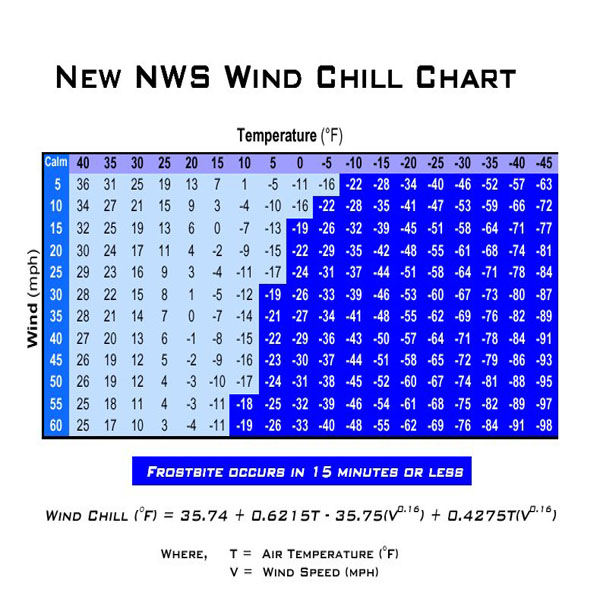
\includegraphics[width=3in]{../../modules/multivariable-functions/pictures/windchill2.jpg}
\end{itemize}
\end{frame}
\begin{frame}
\begin{itemize}
\item Another example is the Income Tax Table. Explain what the
input and output variables are in that case.
\end{itemize}
\end{frame}
\subsection{Analytical description} 
\begin{frame}\frametitle{Analytical description of multivarible function}

\begin{itemize}
\item Numerical data has output data for selected inputs only. 
\item<2-> If output is not tabulated for given input we need to approximate.
\item<3-> This is done by inter/extrapolation from given information. 
\item<4-> It would be better to have procedure to determine output from any reasonable input. 
\item<5-> This would be an \emph{analytical} description of the function. 
\item<5-> By analytical description we mean giving a procedure to compute the value of the function:
\begin{itemize}
\item<6-> via formula or
\item<7-> via another algorithmic procedure.
\end{itemize}

\end{itemize}
\end{frame}
\begin{frame}\frametitle{From numerical to analytical description}

\begin{itemize}
\item<1-> One way is to try to guess a formula that fits approximately the input data. 
\item<2-> For wind chill, one such formula is:
\[
W(T,v)= 35.74+0.6215 T - 35.75 v^{0.16} +0.4275 Tv^{0.16}
\]
with $W$ and $T$ in Fahrenheit and $v$ in $mph$.
\item<3-> A proper mathematical model requires that we
\begin{itemize}
\item<4-> compute unknown output for some input and 
\item<5-> make a new measurement and compare with the model's output to see if model gives correct prediction.
\end{itemize}
\item<6-> Constructing mathematical models to fit numerical data (approximately) is the subject of ``\alert<8>{Approximation theory}''. 
\item<7-> Mathematicians dealing with ``\alert<8>{approximation theory}'' are often called ``applied mathematicians''.
\item<8-> The \alert<8>{above terms} are not precisely defined and not fully agreed upon. 
\end{itemize}
\end{frame}
\begin{frame}
\begin{itemize}
\item For the Cobb-Douglas production function: economic analysis motivates properties such function should have. 
\item One formula (model) with these properties is:
\[
P(K,L) = cL^a K^{1-a}\; ;
\]
where $a$ is a parameter between $0$ and $1$. 
\item While the function $P$ depends on three variables $a$, $L$, and $K$, we treat them differently: we consider $a$ to be a parameter of the model; once we decide on the value of $a$, we treat it as a constant.
\item The transition formulas from spherical to rectangular coordinates are a derived via geometric reasoning.
\end{itemize}
\end{frame}

\begin{frame}
\begin{itemize}
\item An important class of functions of several variables is the class of polynomial functions. Polynomials of degree one are
\begin{align*}
f(x,y) = & ax+by+c \\
g(x,y,z) = & ax+by+cz+d  \; ,
\end{align*}
and polynomials of degree two are
\begin{align*}
f(x,y) = & \; a_{11}x^2+a_{12}xy+a_{22}y^2+ a_1 x + a_2 y + a_0 \\
g(x,y,z) = & \; a_{11} x^2 + a_{22}y^2 + a_{33}z^2 + a_{12}xy + a_{13}xz+a_{23}yz + \\
& + a_1 x + a_2 y + a_3 z + a_0
\end{align*}
where the $a_{ij}$'s are real numbers.
\end{itemize}
\end{frame}
\begin{frame}
\begin{itemize}
\item The formula for electric force is given by laws of physics: the magnitude of the force is directly proportional to the charges $q$, $Q$, and inversely proportional to the square of the distance between them. The force acts along the line joining the two points, attracts $q$ to $Q$ if the charges have different sign and rejects $q$ from $Q$ if the charges have the same sign. The mathematical translation is
\[
\textbf{E}(q, Q, \textbf{r}, \epsilon) = \frac{\epsilon q Q}{|\textbf{r}|^3} \textbf{r}\; ,
\]
where $\epsilon$ is a proportionality constant, depending on the medium the charges are placed in.
\end{itemize}
\end{frame}

\section{Graphical descriptions}
\subsection{Functions of two variables}
\begin{frame}
\begin{itemize}
\item An analytical description is technically best, but not easy to interpret.
\item If output is a scalar, where does the function attain its extreme values (maxima, minima)?  
\item How do values change for nearby points - are they decreasing, increasing, how fast?
\item We will learn to decode this information from the analytical descriptions.
\item Even so, ``a picture is worth a thousand words (and, say, 10 f-las)''.
\end{itemize}
\end{frame}

\begin{frame}
\begin{center}
\psset{xunit=1cm,yunit=1cm}
\begin{pspicture}(-3,-3)(3,5.5)
\renewcommand{\fcScreen}{[-1 -1 -0.4] 0}
\fcAxesIIId{5}{5}{5}
\fcPlotIIId[linewidth=0.3pt, linecolor=blue]{iterationsX=50, iterationsY=50}{-4}{-4}{4}{4}{ x 3 exp x y 4 exp mul add x 5 div sub 10 mul 2.729 x dup mul y dup mul add neg exp mul 2.729 x 1.225 sub dup mul y dup mul add neg exp add}
\rput[t](-3,5.3){Graph of a scalar function.}
\end{pspicture}
\end{center}

\end{frame}

\begin{frame}\frametitle{Graph of a function}
\begin{itemize}
\item For one variable function, $y=f(x)$, the graph of $f$ is a set of points in $\RR^2$: the set of points $(x,y)$ such that $y=f(x)$.
\item Example: if $f(x) = x^2$, then  $(3,9)$ is on the graph, because $9=3^2$, but $(2,5)$ is not because $5 \neq 2^2$.
\item We can extend this graphical representation for functions with two dimensional input and one dimensional (scalar) output. 
\item The \emph{graph} of the function $f\colon D \to \RR$, where $D$ is a region in $\RR^2$, is the set of points $P(x,y,z)$ in $\RR^3$ whose coordinates satisfy the condition 
\[
z=f(x,y)\quad .
\]
\item For example, the graph of $f(x,y) = 2x-y+3$ is the set
\[
\{ (x,y,z) \, | \, z= 2x-y+3\} \Longrightarrow \text{ plane } 2x-y-z+3=0 \; .
\]

\end{itemize}

 



\end{frame}

\subsection{Slices and level curves}
%\begin{comment}
\begin{frame}
\frametitle{A motivating example}
$
\displaystyle g(x,y) =x^2+2y^2
$ 

\begin{itemize}
\item What does the graph $\Gamma$ of $g$ look like?
\item $\Gamma$ = points in $\RR^3$ such that $z=x^2+2y^2$. The set is not a plane: what does it look like?
\item To answer look at sections. Use imaginary CT scan to cut the graph; assemble resulting sections into a graph.
\end{itemize}

\vskip 10cm
\end{frame}

\begin{frame}
\frametitle{A motivating example}
$
g(x,y) =x^2+2y^2
$

\begin{columns}[c]
\column{0.4\textwidth}
\centering


\psset{xunit=0.8cm, yunit=0.8cm}
\begin{pspicture}(-3,-2)(3,4)
\tiny
\renewcommand{\fcScreen}{[-1 1 -0.5] -1}
\psline[linecolor=red!1](3, 4)(3.01,4.01)%
\psline[linecolor=red!1](-3, -1)(-3.01,-1.01)%
\uncover<2-5,9>{\fcParallelogramIIId{[1 -1.2 -0.5]}{[1 1.2 -0.5]}{[1 1.2 4]}}%
\uncover<6>{\fcParallelogramIIId{[0 -1.2 -0.5]}{[0 1.2 -0.5]}{[0 1.2 4]}} % 
\uncover<7>{\fcParallelogramIIId{[0.333333 -1.2 -0.5]}{[0.333333 1.2 -0.5]}{[0.333333 1.2 4]}} %
\uncover<8>{\fcParallelogramIIId{[0.666666 -1.2 -0.5]}{[0.666666 1.2 -0.5]}{[0.666666 1.2 4]}} %
\fcAxesIIId{3}{3}{3}
\uncover<11->{\fcLineIIId[arrows=->, linecolor=black]{[0 0 0]}{[-3 0 0]}}
%parabola at x=1
\uncover<4-5,9->{\fcCurveIIId{-1.2}{1.2}{1 t 2 t t mul mul 1 add }} %
\uncover<5,9,10,12>{\fcDotIIId{[1 0 1]}} %
\uncover<2-5,9>{%
\fcDotIIId[linecolor=black]{[1 0 0]} %
\fcPutIIId[t]{[1 0 -0.3]}{$~~a$}%
} %
\uncover<5>{\fcPutIIId[bl]{[1 0 1.3]}{$~~~~\left(a,0,a^2\right)$}}%
%parabola at x=0
\uncover<6,10->{\fcCurveIIId{-1.2}{1.2}{0 t 2 t t mul mul 0 add }}
\uncover<6,10,12>{\fcDotIIId{[0 0 0]}}
\uncover<6>{ %
\fcDotIIId[linecolor=black]{[0 \space 0 0]}%
\fcPutIIId[t]{[0 0 -0.3]}{$~~a=0$}%
} %
%parabola at x=1/3
\uncover<7>{\fcCurveIIId{-1.2}{1.2}{0.333333 t 2 t t mul mul 0.333333 dup mul add }}
\uncover<7>{\fcDotIIId{[0.333333 0 0.333333 0.333333 mul]}}
\uncover<7>{ %
\fcDotIIId[linecolor=black]{[0.333333 0 0]}%
\fcPutIIId[t]{[0.333333 0 -0.3]}{$~~a$}%
}
%parabola at x=1/2
\uncover<10->{\fcCurveIIId{-1.2}{1.2}{0.5 t 2 t t mul mul 0.5 dup mul add }}
\uncover<10>{\fcDotIIId{[0.5 0 0.5 dup mul]}}
%parabola at x=2/3
\uncover<8>{\fcCurveIIId{-1.2}{1.2}{0.666666 t 2 t t mul mul 0.666666 dup mul add }}%
\uncover<8>{\fcDotIIId{[0.666666 0 0.666666 0.666666 mul]}}
\uncover<8>{ %
\fcDotIIId[linecolor=black]{[0.666666 0 0]}%
\fcPutIIId[t]{[0.666666  0 -0.3]}{$~~a$}%
} %
\uncover<11->{
%\fcCurveIIId{-1.2}{1.2}{-0.333333 t 2 t t mul mul 0.333333 dup mul add }
\fcCurveIIId{-1.2}{1.2}{-0.5 t 2 t t mul mul 0.5 dup mul add }
\fcCurveIIId{-1.2}{1.2}{-1.0 t 2 t t mul mul 1.000000 dup mul add }
}
\uncover<12>{
\fcCurveIIId[linecolor=blue]{-1.5}{1.5}{t 0 t t mul}
\fcDotIIId{[-0.5 0  -0.5 dup mul]}
\fcDotIIId{[-1.000000 0  -1.000000 dup mul]}
}
\end{pspicture}

\uncover<2->{
\psset{xunit=0.5cm, yunit=0.5cm}
\begin{pspicture}(-1.6, -0.9)(1.6,4.38) 
\tiny 
\psframe*[linecolor=cyan!30](! -1.45 -0.75)(! 1.45 4.13)%
\psaxes[ticks=none, labels=none]{<->}(0,0)(-1.35,-0.65)(1.35,4.03)
\fcLabels[$y$][$z$]{1.35}{4.03}

\uncover<6>{
%Function formula: 2 x^{2} 
\psplot[linecolor=\fcColorGraph, plotpoints=1000]{-1.2}{1.2}{x 2 exp 2 mul }
\fcFullDot{0}{0}
}

\uncover<7>{
%Function formula: 2 x^{2}+\frac{1}{9} 
\psplot[linecolor=\fcColorGraph, plotpoints=1000]{-1.2}{1.2}{ 0.111111 x 2 exp 2 mul add }
\fcFullDot{0}{0.111111}
}
\uncover<8>{
%Function formula: 2 x^{2}+\frac{4}{9} 
\psplot[linecolor=\fcColorGraph, plotpoints=1000]{-1.2}{1.2}{ 0.444444 x 2 exp 2 mul add }
\fcFullDot{0}{0.444444}
}
\uncover<3-5, 9->{ %
%Function formula: 2 x^{2}+1 
\psplot[linecolor=\fcColorGraph, plotpoints=1000]{-1.2}{1.2}{ 1 x 2 exp 2 mul add } %
} %
\uncover<5, 9->{\fcFullDot{0}{1}} %
\end{pspicture} 

The plane $x=a$.
} % uncover end

\column{0.6\textwidth}
\begin{itemize}
\item<2-> Cut by vertical planes $x=a$, $a$-constant, parallel to the $Oyz-$plane.
\item<3-> In other words, treat $x$ as constant and study the f-n $y\to z= a^2+2y^2=g(a,y) $.

\item<4-> The cross-sections are the curves:
$
\displaystyle \{(a, y, z)\quad \text{where } z=a^2+2y^2\}
$
\item<5-> These are parabolas lying inside the plane $x=a$ with vertices at $\left(a,0,a^2\right)$. 

\item<6-> As $a$ moves away from $0$, the parabola vertex rises. 
\item<12-> The vertices traverse the curve given by $\{ (a, 0, a^2) \}$.
\end{itemize}
\end{columns}

\vskip 10 cm
\end{frame}
%\end{comment}

%\begin{comment}
\begin{frame}
\frametitle{A motivating example}
$
g(x,y) =x^2+2y^2
$

\begin{columns}[c]
\column{0.4\textwidth}
\centering
\psset{xunit=0.8cm, yunit=0.8cm}
\begin{pspicture}(-3,-2)(3,4)
\tiny
\renewcommand{\fcScreen}{[-1 1 -0.5] -1}
\psline[linecolor=red!1](3, 4)(3.01,4.01)%
\psline[linecolor=red!1](-3, -1)(-3.01,-1.01)%
%parabola at y=1
\uncover<1-3,7>{\fcParallelogramIIId{[-1  1 -0.5]}{[1 1 -0.5]}{[1 1 4]}}%
\uncover<1-3,7>{ %
\fcDotIIId[linecolor=black]{[0 1 0]}%
\fcPutIIId[t]{[0 1 -0.3]}{$~~a$}%
} %
\uncover<3,7->{\fcCurveIIId{-1}{1}{ t 1 2 t t mul mul 1 dup mul 2 mul add}} %

%parabola at y=0
\uncover<4>{\fcParallelogramIIId{[-1  0 -0.5]}{[1 0 -0.5]}{[1 0 4]}}%
\uncover<4>{ %
\fcDotIIId[linecolor=black]{[0 0 0]}%
\fcPutIIId[t]{[0 0 -0.3]}{$~~a$}%
} %
\uncover<4,8->{\fcCurveIIId{-1}{1}{t 0 2 t t mul mul 0 dup mul 2 mul add}} %

%parabola at y=1/3
\uncover<5>{\fcParallelogramIIId{[-1  0.333333 -0.5]}{[1 0.333333 -0.5]}{[1 0.333333 4]}}%
\uncover<5>{ %
\fcDotIIId[linecolor=black]{[0 0.333333 0]}%
\fcPutIIId[t]{[0 0.333333 -0.3]}{$~~a$}%
} %
\uncover<5>{\fcCurveIIId{-1}{1}{t 0.333333 2 t t mul mul 0.333333 dup mul 2 mul add}} %

%parabola at y=2/3
\uncover<6>{\fcParallelogramIIId{[-1  0.666666 -0.5]}{[1 0.666666 -0.5]}{[1 0.666666 4]}}%
\uncover<6>{ %
\fcDotIIId[linecolor=black]{[0 0.666666 0]}%
\fcPutIIId[t]{[0 0.666666 -0.3]}{$~~a$}%
} %
\uncover<6,8->{\fcCurveIIId{-1}{1}{t 0.666666 2 t t mul mul 0.666666 dup mul 2 mul add}} %

\fcAxesIIId{3}{3}{3}%
\uncover<9->{
\fcLineIIId[arrows=->]{[0 0 0]}{[0 -3 0]} %
\fcCurveIIId{-1}{1}{t -0.666666 2 t t mul mul 0.666666 dup mul 2 mul add} %
\fcCurveIIId{-1}{1}{t -1 2 t t mul mul 1 dup mul 2 mul add} %
}
\uncover<10->{
\fcCurveIIId[linecolor=blue]{-1.2}{1.2}{0 t 2 t t mul mul }
\fcDotIIId{[0 0 0]}
\fcDotIIId{[0 -0.5 0.5]}
\fcDotIIId{[0 0.5 0.5]}
\fcDotIIId{[0 1 2]}
\fcDotIIId{[0 -1 2]}
}
\end{pspicture}

\uncover<1->{
\psset{xunit=0.5cm, yunit=0.5cm}
\begin{pspicture}(-1.6, -0.9)(1.6,4.38) 
\tiny 
\psframe*[linecolor=cyan!30](! -1.45 -0.75)(! 1.45 4.13)%
\psaxes[ticks=none, labels=none]{<->}(0,0)(-1.35,-0.65)(1.35,4.03)
\fcLabels[$x$][$z$]{1.35}{4.03}
\uncover<4>{
%Function formula: 2 x^{2} 
\psplot[linecolor=\fcColorGraph, plotpoints=1000]{-1}{1}{x 2 exp 2 mul }
}%
\uncover<5>{%
%Function formula: 2 x^{2}+\frac{2}{9} 
\psplot[linecolor=\fcColorGraph, plotpoints=1000]{-1}{1}{ 2 9 div x 2 exp 2 mul add }%
}%
\uncover<6>{%
%Function formula: 2 x^{2}+2*\frac{4}{9} 
\psplot[linecolor=\fcColorGraph, plotpoints=1000]{-1}{1}{ 8 9 div x 2 exp 2 mul add }%
}%
\uncover<3, 7->{%
%Function formula: 2 x^{2}+1 
\psplot[linecolor=\fcColorGraph, plotpoints=1000]{-1}{1}{ 2 x 2 exp 2 mul add }%
}%
\end{pspicture} 

The plane $x=a$.
} % uncover end

\column{0.6\textwidth}
\begin{itemize}
\item<1-> Similarly, cut by vertical planes $y=a$, i.e., planes parallel to the $Oxz$ plane.

\item<2-> In other words, treat $y$ as constant and study the f-n $z=g(x,a) = x^2+2a^2$.

\item<3-> The cross-sections are the curves  $\{ (x,a,z) \text{  where  } z= x^2+2a^2\}$. These are parabolas lying inside the plane $y=a$. 
\item<8-> $\Rightarrow$ the vertical sections along both the $x$ and $y$ axes are parabolas.
\item<10-> The vertices are rising as we move away from the origin.
\end{itemize}
\end{columns}

\vskip 10 cm
\end{frame}
%\end{comment}


%\begin{comment}
\begin{frame}

\frametitle{A motivating example}
$
g(x,y) =x^2+2y^2
$

\begin{columns}[c]
\column{0.4\textwidth}
\centering
\psset{xunit=0.8cm, yunit=0.8cm}
\begin{pspicture}(-3,-2)(3,4)
\tiny
\renewcommand{\fcScreen}{[-1 1 -0.5] -1}
\psline[linecolor=red!1](3, 4)(3.01,4.01)%
\psline[linecolor=red!1](-3, -2)(-3.01,-2.01)%
\uncover<1-2>{ %
\fcParallelogramIIId{[-2.5  -2.5 1]}{[2.5 -2.5 1]}{[2.5 2.5 1]}
\fcDotIIId[linecolor=black]{[0 0 1]}%
\fcPutIIId[tl]{[0 0 1]}{$~~a$}%
} %
\uncover<3>{ %
\fcParallelogramIIId{[-2.5  -2.5 -1]}{[2.5 -2.5 -1]}{[2.5 2.5 -1]}
\fcDotIIId[linecolor=black]{[0 0 -1]}%
\fcPutIIId[tl]{[0 0 -1]}{$~~a$}%
} %
\uncover<4>{ %
\fcParallelogramIIId{[-2.5  -2.5 0]}{[2.5 -2.5 0]}{[2.5 2.5 0]}
} %
\uncover<5>{ %
\fcParallelogramIIId{[-2.5  -2.5 0.5]}{[2.5 -2.5 0.5]}{[2.5 2.5 0.5]}
} %
\uncover<6>{ %
\fcParallelogramIIId{[-2.5  -2.5 1]}{[2.5 -2.5 1]}{[2.5 2.5 1]}
} %
\uncover<7>{ %
\fcParallelogramIIId{[-2.5  -2.5 1.5]}{[2.5 -2.5 1.5]}{[2.5 2.5 1.5]}
} %
\uncover<8>{ %
\fcParallelogramIIId{[-2.5  -2.5 2]}{[2.5 -2.5 2]}{[2.5 2.5 2]}
} %

\fcAxesIIId{3}{3}{3}%
\fcLineIIId[arrows=->]{[0 0 0]}{[0 -3 0]} %
\fcLineIIId[arrows=->]{[0 0 0]}{[-3 0 0]} %
\fcLineIIId[arrows=->]{[0 0 0]}{[0 0 -1.5]} %

\uncover<4>{\fcDotIIId{[0 0 0]}}
\uncover<5,9->{ % 
\fcCurveIIId{ 0}{6.2832}{t 360 mul cos 0.500 sqrt mul t 360 mul sin 0.500 2 div sqrt mul 0.5} 
}
\uncover<5>{\fcDotIIId[linecolor=black]{[0 0 0.5]}}
\uncover<6,9->{ % 
\fcCurveIIId{ 0}{6.2832}{t 360 mul cos 1 sqrt mul t 360 mul sin 1 2 div sqrt mul 1} 
}
\uncover<6>{\fcDotIIId[linecolor=black]{[0 0 1]}}
\uncover<7,9->{ % 
\fcCurveIIId{ 0}{6.2832}{t 360 mul cos 1.5 sqrt mul t 360 mul sin 1.5 2 div sqrt mul 1.5} 
}
\uncover<7>{\fcDotIIId[linecolor=black]{[0 0 1.5]}}
\uncover<8,9->{ % 
\fcCurveIIId{ 0}{6.2832}{t 360 mul cos 2.0 sqrt mul t 360 mul sin 2.0 2 div sqrt mul 2.0} 
}
\uncover<8>{\fcDotIIId[linecolor=black]{[0 0 2.0]}}

\uncover<10->{
\fcCurveIIId[linewidth=1pt, linecolor=blue]{-1.414214 }{1.414214}{t 0 t t mul}
\fcCurveIIId[linewidth=1pt, linecolor=blue]{-1}{1}{0 t t t 2 mul mul}
}
\uncover<11->{
\fcCurveIIId[linewidth=2pt, linecolor=\fcColorGraph]{ 0}{6.2832}{t 360 mul cos 0.500 sqrt mul t 360 mul sin 0.500 2 div sqrt mul 0.5} 
\fcCurveIIId[linewidth=2pt, linecolor=\fcColorGraph]{ 0}{6.2832}{t 360 mul cos 1 sqrt mul t 360 mul sin 1 2 div sqrt mul 1} 
\fcCurveIIId[linewidth=2pt, linecolor=\fcColorGraph]{ 0}{6.2832}{t 360 mul cos 1.5 sqrt mul t 360 mul sin 1.5 2 div sqrt mul 1.5} 
\fcCurveIIId[linewidth=2pt, linecolor=\fcColorGraph]{ 0}{6.2832}{t 360 mul cos 2.0 sqrt mul t 360 mul sin 2.0 2 div sqrt mul 2.0} 
}
\end{pspicture}

\uncover<2->{
\psset{xunit=0.4cm, yunit=0.4cm}
\begin{pspicture}(-3.228413, -1.814212)(3.228427,1.914212) 
\tiny 
\psframe*[linecolor=cyan!30](! -3.078413 -1.664212)(! 3.078427 1.664212)%
\psaxes[ticks=none, labels=none]{<->}(0,0)(-2.978413,-1.564212) (2.978427,1.564212)
\fcLabels[$x$][$y$]{2.978427}{1.564212}
\uncover<4>{
\fcFullDot{0}{0}
}
\uncover<5>{
%Calculator input: plotCurve{}\left(\frac{\sqrt{2}}{2} \cos{}t, \frac{1}{2} \sin{}t, 0, 2 \pi\right)
\parametricplot[linecolor=\fcColorGraph, plotpoints=1000]{0}{6.28319}{t 57.29578 mul cos 0.707107 mul t 57.29578 mul sin 0.5 mul }
}
\uncover<6>{
%Calculator input: plotCurve{}\left(\cos{}t, \frac{\sqrt{2}}{2} \sin{}t, 0, 2 \pi\right)
\parametricplot[linecolor=\fcColorGraph, plotpoints=1000]{0}{6.28319}{t 57.29578 mul cos t 57.29578 mul sin 0.707107 mul }
}
\uncover<7>{
%Calculator input: plotCurve{}\left(\frac{\sqrt{2}\sqrt{3}}{2} \cos{}t, \frac{\sqrt{3}}{2} \sin{}t, 0, 2 \pi\right)
\parametricplot[linecolor=\fcColorGraph, plotpoints=1000]{0}{6.28319}{t 57.29578 mul cos 1.224745 mul t 57.29578 mul sin 0.866025 mul }
}
\uncover<8->{
%Calculator input: plotCurve{}\left(\sqrt{2} \cos{}t, \sin{}t, 0, 2 \pi\right)
\parametricplot[linecolor=\fcColorGraph, plotpoints=1000]{0}{6.28319}{t 57.29578 mul cos 1.414214 mul t 57.29578 mul sin }
}
\end{pspicture} 

$x^2+2y^2= \only<1-3>{a} \only<4>{\alert<4>{0}}$, \only<1-3>{\alert<5>{$a<0$}}\only<5->{\alert<5>{$a>0$}}.
}

\column{0.6\textwidth}
\begin{itemize}
\item<1-> For horizontal sections keep constant the output variable, $z=a$.
\item<2-> When we intersect with $z=a$ we get the curve with equations $x^2+2y^2=a$, $z=a$.
\item<3-> For $a<0$ intersection is empty.
\item<4-> For $a=0$ intersection is $(0,0,0)$.
\item<5-> For $a>0$ intersection is an ellipse. 
\item<10-> Figure is called ellipsoidal paraboloid.
\end{itemize}
\uncover<11->{
\begin{definition}
The sets $\{ (x,y,a)| g(x,y)=a\}$ are called \alert<11>{level curves} of the function $g$.
\end{definition}
}
\end{columns}

\vskip 10 cm
\end{frame}
\begin{frame}

\begin{itemize}
\item 
You should be familiarized with level curves if you have ever seen a topographic map or from weather reports on the tv. 
\item What are the functions in those cases?
\end{itemize} 
\end{frame}
%\end{comment}
\subsection{Level sets}
\begin{frame}
\begin{itemize}
\item<1-> Previously we considered functions $\alertNoH{2,6}{z}= g(\alertNoH{3,5}{x,y})$  \alertNoH{2}{with scalar output} and \alertNoH{3}{two dimensional input}.
\item<4-> The graphs of such functions live in $\RR^3 = \RR^{\alertNoH{5}{2} +\alertNoH{6}{1}}$.
\item<5-> \alertNoH{5}{2 dimensions} were used to represent the input.
\item<6-> \alertNoH{6}{1 dimension} was used to represent the output.
\item<7-> To represent functions with 3 dimensional input (3 variables) and scalar output: need  $3+1=4$ dimensions.
\item<8-> That's difficult for eyes used to visualizing physical 3d- space.
\item<9-> Instead: label the level sets of the function with color or other means to indicate value.
\item<10-> In this way we represent the f-n graphically using dimension equal to the number of input variables.
\end{itemize}
\end{frame}
\begin{frame}
\frametitle{Example}
\begin{columns}
\column{0.4\textwidth}
\psset{xunit=0.4cm, yunit=0.4cm}
\begin{pspicture}(-4,-7)(6,10)
\renewcommand{\fcScreen}{[-1 1 -0.7] -1}
\fcBoundingBox{-4}{-8.5}{4}{10.5}
\tiny
\fcAxesIIIdFull{5}{5}{5}%
\uncover<5->{%
%d=4
\fcParallelogramIIId[linecolor=cyan!90]{[-2 -2 -8]}{[-2 3 -3]}{[5 -2 -1]}%
\fcPutIIId[l]{[2 2 0]}{$~~d=4$}%
\fcLineIIId{[0 0 0]}{[0 0 -4]}
\fcLineIIId{[0 0 0]}{[4 0 0]}
}%
\uncover<6->{%
%d=2
\fcParallelogramIIId[linecolor=cyan!70]{[-2 -2 -6]}{[-2 3 -1]}{[5 -2 1]}%
\fcPutIIId[l]{[2 2 2]}{$~~d=2$}%
\fcLineIIId{[0 0 0]}{[0 2 0]}
\fcLineIIId{[0 0 0]}{[2 0 0]}
\fcLineIIId{[0 0 0]}{[0 0 -2]}
}%
\uncover<7->{%
%d=0
\fcParallelogramIIId[linecolor=cyan!50]{[-2 -2 -4]}{[-2 3 1]}{[5 -2 3]}%
\fcPutIIId[l]{[2 2 4]}{$~~d=0$}%
\fcLineIIId{[0 0 0]}{[0 0 4]}
\fcLineIIId{[0 0 0]}{[-4 0 0]}
\fcLineIIId{[0 0 0]}{[0 -4 0]}
}%
\uncover<8->{%
%d=-2
\fcParallelogramIIId[linecolor=cyan!30]{[-2 -2 -2]}{[-2 3 3]}{[5 -2 5]}%
\fcPutIIId[l]{[2 2 6]}{$~~d=-2$}%
\fcLineIIId{[0 0 2]}{[0 0 4]}%
\fcLineIIId{[-2 0 0]}{[-4 0 0]}%
\fcLineIIId{[0 -2 0]}{[0 -5 0]}%
}%
\uncover<9->{%
%d=-4
\fcParallelogramIIId[linecolor=cyan!10]{[-2 -2 0]}{[-2 3 5]}{[5 -2 7]}%
\fcPutIIId[l]{[2 2 8]}{$~~d=-4$}
\fcPutIIId[l]{[2 2 6]}{$~~d=-2$}%
\fcLineIIId{[0 0 4]}{[0 0 5]}%
\fcLineIIId{[-4 0 0]}{[-5 0 0]}%
}%
\fcAxesIIIdFull[arrows=->, linestyle=dotted, dash=1pt]{5}{5}{5}
\end{pspicture}

\column{0.6\textwidth}
\begin{itemize}
\item<1-> Let $f(x,y,z) = x+y-z$.
\item<2-> The graph consists of the quadruples $(x,y,z,w)$ in $\RR^4$ such that $w = x+y-z$. Can't plot that graphically (yet).
\item<3-> However, can represent with labeled level sets.
\item<4-> The level set $f(x,y,z) = d$ is the surface $x+y-z = d$ in $\RR^3$, and that surface is a plane.
\item<5-> For varying values of $d$ we plot the level set.
$f(x,y,z) =d \onlyNoH{5}{=4}\onlyNoH{6}{=2} \onlyNoH{7}{=0}\onlyNoH{8}{=-2}
\onlyNoH{9}{=-4}$.

Darker color = larger $d$.
\end{itemize}
\end{columns}

\end{frame}

\begin{frame}
To understand surfaces in space we need the following.
\begin{remark} The level set $f(x,y,z)=0$ for the function
%
$$f(x,y,z) = ax+by-z+d$$
%
is the same as the graph of the function $g(x,y) = ax+by+c$.
\end{remark}
\begin{itemize}
\item<2-> Graph surfaces can always be represented as level surfaces
\item<3-> The converse is not true: level surfaces can't always be represented as graph surfaces.
\item<4-> Example: a sphere centered at the origin is the
level surface of $f(x,y,z) = x^2+y^2+z^2$ but it ``fails the vertical line test in all directions'', so it cannot be globally represented as a graph surface, no matter how we change the coordinate system.
\item<5-> We'll show that under reasonable assumptions, level surfaces can \emph{locally} be described as graph surfaces.
\end{itemize}
\end{frame}

\subsection{Vector Fields}
\begin{frame}
\frametitle{Vector fields}
\begin{itemize}
\item \emph{Vector fields} are functions with multidimensional input and output.
\item Input is point in space; output is a vector, which we plot as a vector with a tail at the input point.
\item Examples
\begin{itemize}
  \item Velocity of fluid/air at given point;
  \item Electric force per unit of charge;
  \item Gravitational field;
  %\item Fundamental directions $\textbf{e}_\rho$, $\textbf{e}_\phi$, $\textbf{e}_\theta$, $\textbf{e}_r$
\end{itemize}
\end{itemize}
\end{frame}

\begin{frame}
\frametitle{Coordinate representation of vector fields}

\begin{itemize}
\item<1-> In rectangular coordinates a vector field $\textbf{F}$ can
be decomposed along the fundamental directions:
$$
\textbf{F}(x,y,z) = F_1(x,y,z) \textbf{i} + F_2(x,y,z) \textbf{j} + F_3(x,y,z) \textbf{k} \; .
$$
\item<2-> For regions in the plane 2-dim vector fields are defined in a similar fashion: as function from subsets of $\mathbb R^2$ to $\RR$:
$$
\textbf{F}(x,y) = F_1(x,y) \textbf{i} + F_2(x,y) \textbf{j}
$$


\end{itemize}
\end{frame}
\begin{frame}
\begin{itemize}
\item<1-> Example: define the vector field $\textbf{e}_r$ on $\mathbb{R}^2 \setminus \{ (0,0)\}$ via
$
\textbf{e}_r = \cos\theta\, \textbf{i} +
\sin\theta \,\textbf{j} = \frac{x}{r} \, \textbf{i} +
\frac{y}{r} \, \textbf{j} = \frac{x}{\sqrt{x^2+y^2}} \,
\textbf{i} + \frac{y}{\sqrt{x^2+y^2}} \, \textbf{j}
$

\item<2-> Similarly define the vector field $\textbf{e}_{\theta}$ by:
$\textbf{e}_\theta = -\sin\theta\, \textbf{i} +
\cos\theta \,\textbf{j} = -\frac{y}{r} \, \textbf{i} +
\frac{x}{r} \, \textbf{j} = -\frac{y}{\sqrt{x^2+y^2}} \,
\textbf{i} + \frac{x}{\sqrt{x^2+y^2}} \, \textbf{j} \; .
$

\hfil \hfil\uncover<3->{
\psset{xunit=0.3cm, yunit=0.3cm}
\begin{pspicture}(-5.9,-5.9)(5.9,5.9)
\tiny
\fcAxesStandard{-5.1}{-5.1}{5.1}{5.1}
\fcVectorField[linecolor=blue, arrows=->]{-5}{-5}{11}{11}{1} {1 dict begin /r x x mul y y mul add sqrt def  r 0 eq {0 0} {x r div  y r div} ifelse end}
\end{pspicture}
\psset{xunit=0.3cm, yunit=0.3cm}
~~~ \begin{pspicture}(-5.9,-5.9)(5.9,5.9)
\tiny
\fcAxesStandard{-5.1}{-5.1}{5.1}{5.1}
\fcVectorField[linecolor=blue, arrows=->]{-5}{-5}{11}{11 }{1}{1 dict begin /r x x mul y y mul add sqrt def  r 0 eq {0 0} {-1 y mul r div  x r div} ifelse end}
\end{pspicture}
}
\item<4-> From the picture it is evident what trajectory would be followed by an object that ``\alertNoH{5}{flows along the vector field}''.
\item<5-> By ``\alertNoH{5}{flowing}'' we mean an object whose \alertNoH{5}{velocity} at each point is given by \alertNoH{5}{the value of the field}.
\end{itemize}
\end{frame}

%\begin{frame}
Similar to decomposition in rectangular coordinates we can decompose a vector field along fundamental vectors corresponding to other coordinate systems. Things are a bit trickier, since the fundamental vectors change from
point to point.

In particular, a planar vector field can be written in terms of
$\textbf{e}_r$ and $\textbf{e}_\theta$:
%
$$\textbf{X}(r,\theta) = X_1(r,\theta) \textbf{e}_r\, +
X_2(r,\theta) \textbf{e}_\theta\; .$$
%
For example, if $X(P) = \textbf{i}$, then
%
$$X(r,\theta) = \cos\theta \,\textbf{e}_r\,
-\sin\theta \, \textbf{e}_\theta\; .$$
\end{frame} %<- this remark needs to be rewriten using standard mathematical language. At the moment this slide present a omelette of displacement vectors, vector fields, graphs of vector fields and vectors. 
}


\lect{2014}{Lecture 7}{7}{
\section{Surfaces}

\subsection{Implicit functions}
\begin{frame}
\begin{itemize}
\item A surface $S$ can be given in two different ways:

\begin{itemize}
\item<2-> Implicit form, as a \emph{level surface}: $$F(x,y,z) = 0$$.
\item<3-> Explicit form, as a \emph{graph surface}:
\[z=f(x,y) \Longrightarrow 
\left\{ \begin{array}{ll}
x = & u \\
y = & v \\
z = & f(u,v)
\end{array} \right.
\]
\end{itemize}
\item<4-> A graph surface $z=f(x,y)$ can always be represented as a level surface:
\[
z=f(x,y) \Longleftrightarrow F(x,y,z) =0 \quad \text{ for } \quad F(x,y,z) = z-f(x,y)\; .
\]
\end{itemize}
\end{frame}
\begin{frame}
\begin{question}
Can a given level surface be represented as a graph surface?
\end{question}
\begin{itemize}
\item<2-> \alert<1->{Globally}, level surfaces are \alert<1->{cannot} be represented as graph surfaces.

\item<3-> Example: $x^2+y^2+z^2= 1$: can't solve for $z$ globally. \uncover<4->{Informally, $z=\pm\sqrt{1-x^2-y^2}$, however this is \alert<1->{not a function} if we can't decide on choice of $+$ or $-$. }
\item<5-> \alert<1->{Locally, } with additional requirements, a level surface \alert<1->{can} be represented as graph surfaces. 

\begin{itemize}
\item<6-> Near $P(0,0,1)$, the surface is the graph surface of $z = \sqrt{1-x^2-y^2}$.
\item<7-> Near $P(1, 0, 0)$, the surface is not a graph surface w.r.t. to $z$.
\end{itemize} 
\end{itemize}
\end{frame}

\begin{frame}
\begin{itemize}
\item<1-> Let $F(x,y,z)$- function, let $P(x_0,y_0,z_0)$ - point in the domain of $F$.
\item<2-> Let $F(x_0,y_0,z_0)=k$.
\item<3-> We say the level surface is a graph surface around $P$ if there is a function $z=f(x,y)$ such that:
\begin{itemize}
\item<4-> $f$ is defined on an open disk $D$ around $(x_0,y_0)$;
\item<5-> $f(x_0,y_0) = z_0$;
\item<6-> $F(x,y,f(x,y)) = 0$ for all $(x,y)$ in the disk $D$.
\end{itemize}
\item<7-> If the level surface is a graph surface, we say that the equation $F(x,y,z) = k$ \alert<1->{implicitly} defines $z=f(x,y)$ satisfying the condition $f(x_0,y_0) = z_0$.

\end{itemize}
\end{frame}


\begin{frame}
\begin{itemize}
\item The equation $x^2+y^2+z^2 = 1$ implicitly defines $z=\sqrt{1-x^2 -y^2 }$ as the unique function $z=f(x,y)$ such that

\begin{itemize}
\item $x^2+ y^2+(f(x,y))^2 = 1$ for all $(x,y)$ in a disk around $(0,0)$;
\item $f(0,0) = 1$.
\end{itemize}
\item The equation $x^2+y^2+z^2 = 1$ implicitly defines $z=-\sqrt{1 -x^2- y^2 }$ as the unique function $z=f(x,y)$ such that
%
\begin{itemize}
\item $x^2+ y^2+(f(x,y))^2 = 1$ for all $(x,y)$ in a disk around $(0,0)$;
\item $f(0,0) = -1$.
\end{itemize}
\end{itemize}


\end{frame}
\subsection{Parametrizations}
\begin{frame}
\begin{itemize}
\item So far: focused on functions with scalar output. 
\item<2-> We've seen examples of functions with vectorial output.
\item<3-> Example: vectorial parametric equation of a plane through $P_0(\textbf{r}_0)$, parallel to directions $\fcv{u}$ and $\fcv{v}$ is given by 
\[\textbf{r} = \textbf{r}_0 + s \textbf{u} +
t \textbf{v}\; ,
\]
\item<4-> The function $\fcv{f} \colon \RR^2 \to \RR^3$, $\fcv{f}(s,t) = \fcv{r}_0 + s \fcv{u} + t \fcv{v}$ globally identifies
$\RR^2$ with the plane $\mathcal{P}$.
\item<5-> Each point of $\mathcal{P}$ corresponds uniquely to pair $(s,t)$.
\end{itemize}
\end{frame}

\begin{frame}
\frametitle{Example: parametrization of part of sphere}
\begin{itemize}
\item Consider $f \colon (0,2\pi) \times (0,\pi) \to \RR^3$ given by
\[f(t,s) = (R\sin{s}\cos{t}, R\sin{s}\sin{t},
R\cos{s}) \; .\]

\item<2-> The image of $f$ is a subset of the
sphere of radius $R$ centered at the origin.

\item<3-> Which points of the sphere are not covered
by the image of $f$?
\end{itemize}
\end{frame}

\subsection{Quadric Surfaces}
\begin{frame}
\frametitle{Quadratic surfaces} 
\begin{itemize}
\item The level sets for second degree polynomial functions
\[
f(x,y,z) = \alert<2>{Ax^2+By^2+Cz^2+Dxy+Exz+Fyz} +Gx+Hy+Iz+J.
\]
are called \alert<1->{quadratic surfaces}.
\item<2-> At least one of the \alert<2>{second-degree terms} is required to be non-zero.
\item<3-> The coefficients are allowed to be zero.
\end{itemize}
\end{frame}

\begin{frame}
\frametitle{Canonical forms of quadratic surfaces.}
Through rigid motions (translations and rotations) a quadratic surface can be reduced to one of the two canonical forms.
\begin{itemize}
\item<2-> 
\[  
\begin{array}{rcl} 
Ax^2+By^2+Cz^2+D &=& 0,\\
\uncover<handout: 0|5->{\alert<5>{A(-x)^2+B(-y)^2+C(-z)^2+D} &\alert<5>{=}& \alert<5>{0} ,} 
\end{array} 
\] 
$(A, B, C)\neq (0,0,0)$. 
\uncover<4->{ These quadratics posses central symmetry:} \uncover<5->{\alert<5>{if $(x,y,z)$ belongs to the surface, so does $(-x,-y,-z)$.}}
\item<3-> 
\[
\alert<6>{ Ax^2+By^2+Iz=0,}
\] 
$(A, B)\neq (0,0)$, $\alert<6>{I\neq 0}$.
\uncover<6->{These quadratics do not posses central symmetry.}
\end{itemize}

\uncover<7->{
The canonical forms above are in addition split into sub-forms depending on the sign of $A, B, C, D, I$. 
}

\end{frame}







\begin{frame}
\frametitle{Summary: surfaces of form $Ax^2+By^2+Cz^2+D=0$}
\tiny
\begin{tabular}{|c|c|c|c|c|c|c|c|c|}
\hline
% after \\: \hline or \cline{col1-col2} \cline{col3-col4} ...
A & B & C & D & $x=x_0$ & $y=y_0$ & $z=z_0$ & Example & Name
\\\hline
$>0$ & $>0$ & $>0$ & $>0$ & empty & empty & empty & $x^2+2y^2+3z^2+4=0$ & empty \\
\hline
$>0$ & $>0$ & $>0$ & $=0$ &  &  &  &  &  \\
\hline
$>0$ & $>0$ & $>0$ & $<0$ & ellipse & ellipse & ellipse & $x^2+2y^2+3z^2-4=0$ & Ellipsoid \\
\hline
$>0$ & $>0$ & $=0$ & $>0$ &  &  &  &  &  \\
\hline
$>0$ & $>0$ & $=0$ & $=0$ &  &  &  &  &  \\
\hline
$>0$ & $>0$ & $=0$ & $<0$ &  &  &  &  &  \\
\hline
$>0$ & $>0$ & $<0$ & $>0$ &  &  &  &  &  \\
\hline
$>0$ & $>0$ & $<0$ & $=0$ &  &  &  &  &  \\
\hline
$>0$ & $>0$ & $<0$ & $<0$ &  &  &  &  &  \\
\hline
$>0$ & $=0$ & $=0$ & $>0$ &  &  &  &  &  \\
\hline
$>0$ & $=0$ & $=0$ & $=0$ &  &  &  &  &  \\
\hline
$>0$ & $=0$ & $=0$ & $<0$ &  &  &  &  &  \\
\hline
\end{tabular}

Fill in the rest of the table.
\end{frame}

\begin{frame}
\begin{equation*}
Ax^2+By^2+Iz=0
\end{equation*}

\begin{table}
\begin{tabular}{|c|c|c|c|c|c|c|}
  \hline
  % after \\: \hline or \cline{col1-col2} \cline{col3-col4} ...
  A & B  & $x=x_0$ & $y=y_0$ & $z=z_0$ & Example & Name
  \\
  \hline
  $>0$ & $>0$   & parabola & parabola & ellipse, point, or empty & $x^2+2y^2+3z=0$ & Elliptic paraboloid \\
  \hline
  $>0$ & $=0$ & &  &  &  &   \\
  \hline
  $>0$ & $<0$ &  &  &  &  &   \\
  \hline
\end{tabular}
  \caption{Quadrics without central symmetry}
\end{table}
\bigskip

Fill in the rest of the table.
\end{frame}

\begin{frame}
\frametitle{$Ax^2+By^2+Cz^2+D=0$, $A>0, B>0, C>0, D>0$}
Consider the surface 
$\mathcal C =\{(x,y,z) |Ax^2+By^2+Cz^2+D=0 \}$.

\begin{itemize}
\item Let $A>0, B>0, C>0, D>0$.
\item<2-> Then the surface is the empty set.
\item<3-> Example: 
\[
x^2+2y^2+3z^2+4=0.
\]
\end{itemize}
\vskip 10cm

\end{frame}

\begin{frame}
\frametitle{$Ax^2+By^2+Cz^2+D=0$, $A>0, B>0, C>0, D>0$}
Consider the surface 
$\mathcal C =\{(x,y,z) |Ax^2+By^2+Cz^2+D=0 \}$.


\begin{columns} 
\column{0.4\textwidth}
\psset{xunit=0.5cm, yunit=0.5cm}
\begin{pspicture}(-2,-2)(2, 2)
\tiny
\fcBoundingBox{-2}{-2}{2}{2}
\fcAxesIIId{3}{3}{3}
\uncover<9->{\fcDotIIId{[0 0 -2]}}
\uncover<11->{\fcCurveIIId[linecolor=red]{0}{360}{[3 2 div sqrt t cos mul 1.5 t sin mul -1]}}
\uncover<13->{\fcCurveIIId[linecolor=red]{0}{360}{[2 sqrt t cos mul 3 sqrt t sin mul 0]}}
\uncover<15->{\fcCurveIIId[linecolor=red]{0}{360}{[3 2 div sqrt t cos mul 1.5 t sin mul 1]}}
\uncover<17->{\fcDotIIId{[0 0 2]}}
\fcStartIIIdScene
\only<18->{
\fcEllipsoid{0 0 0 2 sqrt 3 sqrt 2}
}
\fcFinishIIIdScene
\end{pspicture}

\psset{xunit=0.4cm, yunit=0.4cm}
\begin{pspicture}(-2,-2)(2, 2)
\tiny
\fcAxesStandard{-3}{-3}{3}{3}
\fcLabels[$x$][$y$]{3}{3}%
\uncover<9,17>{\fcFullDot{0}{0}}
\uncover<11>{ \parametricplot[linecolor=red]{0}{360}{3 2 div sqrt t cos mul 1.5 t sin mul }}
\uncover<13>{ \parametricplot[linecolor=red]{0}{360}{2 sqrt t cos mul 3 sqrt t sin mul }}
\uncover<15>{ \parametricplot[linecolor=red]{0}{360}{3 2 div sqrt t cos mul 1.5 t sin mul }}
\end{pspicture}

$z=\vphantom{\frac{3}{4}} \parbox{1cm}{ \only<6,7>{\alert<6,7>{ -3}} \only<8,9>{\alert<8,9>{-2} }} \only<10,11>{\alert<10,11>{-1}} \only<12,13>{\alert<12,13>{0}} \only<14,15>{\alert<14,15>{1}} \only<16,17>{\alert<16,17>{2}} $

$
\begin{array}{rl}\frac{1}{2}x^2+\frac{1}{3}y^2&\alert<0>{ =} 1-\frac{z^2}{4}\\
& \uncover<6-17>{\alert<6-17>{=}} \vphantom{\frac{3}{4}} \only<7>{\alert<7>{ -\frac{5}{4}} } \only<9>{\alert<9>{0}} \only<11>{\alert<11>{\frac{3}{4}}} \only<13>{\alert<13>{1}} \only<15>{\alert<15>{\frac{3}{4}}} \only<17>{\alert<17>{0}} \end{array}$ 

\column{0.6\textwidth}
\begin{itemize}
\item Let $A>0, B>0, C>0$, $D<0$. Rescale so $D=-1$.
\item<2-> Set $A=\frac{1}{a^2}$, $B=\frac{1}{b^2}$, $C=\frac{1}{c^2}$.
\item<3-> Surface becomes:
$\left\{(x,y,z)|\left(\frac{x}{a}\right)^2+\left(\frac{y}{b}\right)^2+\left(\frac{y}{z}\right)^2= 1\right\}$.
\item<4-> We illustrate the theory on the example:
$\frac{1}{2}x^2+\frac{1}{3}y^2+\frac{z^2}{4}=1$.
\item<5-> Rewrite:
$\frac{1}{2}x^2+\frac{1}{3}y^2=1-\frac{z^2}{4}$.
\item<5-> The level curves are:
\begin{itemize}
\item<7-> None for $z<2$ and $z>2$.
\item<9-> Two points for $z=\pm 2$.
\item<11-> Ellipses for $z\in (-2,2)$. 
\end{itemize}
\item<18> Figure is called ellipsoid.
\end{itemize}

\end{columns}

\vskip 10cm

\end{frame}
%
\begin{frame}
\frametitle{$Ax^2+By^2+Cz^2+D=0$, $A>0, B>0, C<0, D=0$}


\begin{columns} 
\column{0.4\textwidth}
\psset{xunit=0.3cm, yunit=0.3cm}
\vskip -0.2cm
\begin{pspicture}(-6,-4.5)(6, 5.5)%
\tiny %
\pstVerb{5 dict begin /theValueOfZ 1 def
/theEllipse {t cos 2 mul theValueOfZ mul t sin 2 sqrt mul theValueOfZ mul} def
}%
\renewcommand{\fcScreen}{[-0.4 1 -0.2] 0}%
\fcStartIIIdScene%
\fcBoundingBox{-2}{-2}{2}{2}%
\fcAxesIIIdFullInScene{-3}{-3}{-3}{6}{5}{5}%
\only<21->{%
\fcSurfaceInScene[arrows=(none), linewidth=0.2, linecolor=red, iterationsU=12, iterationsV=3]{0}{0.1}{360}{3}{[u cos 2 mul v mul u sin 2 sqrt mul v mul v ]}{}%
\fcSurfaceInScene[arrows=(none), linewidth=0.2, linecolor=red, iterationsU=12, iterationsV=3]{0}{-3}{360}{-0.1}{[u cos 2 mul v mul u sin 2 sqrt mul v mul v ]}{}%
}%
\only<6->{\fcCurveIIIdInScene[arrows=(none), linecolor=blue, linewidth=1]{0}{360}{1 dict begin /theValueOfZ 1.01 def [t cos 2 mul theValueOfZ mul t sin 2 sqrt mul theValueOfZ mul theValueOfZ] end}}%
\only<7->{\fcCurveIIIdInScene[arrows=(none), linecolor=blue, linewidth=1]{0}{360}{1 dict begin /theValueOfZ 1.01 def [t cos 2 mul theValueOfZ mul t sin 2 sqrt mul theValueOfZ mul theValueOfZ -1 mul] end}}%
\only<9->{\fcCurveIIIdInScene[arrows=(none), linecolor=blue, linewidth=1]{0}{360}{1 dict begin /theValueOfZ 2.01 def [t cos 2 mul theValueOfZ mul t sin 2 sqrt mul theValueOfZ mul theValueOfZ] end}}%
\only<10->{\fcCurveIIIdInScene[arrows=(none), linecolor=blue, linewidth=1]{0}{360}{1 dict begin /theValueOfZ 2.01 def [t cos 2 mul theValueOfZ mul t sin 2 sqrt mul theValueOfZ mul theValueOfZ -1 mul] end}}%
\only<11->{\pstVerb{/theValueOfZ 3.01 def}}%
\only<12->{\fcCurveIIIdInScene[arrows=(none), linecolor=blue, linewidth=1]{0}{360}{1 dict begin /theValueOfZ 3.01 def [t cos 2 mul theValueOfZ mul t sin 2 sqrt mul theValueOfZ mul theValueOfZ] end}}%
\only<13->{\fcCurveIIIdInScene[arrows=(none), linecolor=blue, linewidth=1]{0}{360}{1 dict begin /theValueOfZ 3.01 def [t cos 2 mul theValueOfZ mul t sin 2 sqrt mul theValueOfZ mul theValueOfZ -1 mul] end}}%
\fcFinishIIIdScene%
\only<4->{\fcDotIIId[linecolor=blue]{[0 0 0]}}%
\fcPutIIId[t]{[6 0 0]}{$x$}%
\fcPutIIId[l]{[0 3 0]}{$y$}%
\fcPutIIId[b]{[0 0 5]}{$z$}%
\onlyNoH{17}{\pstVerb{/theValueOfZ 1 def}}%
\onlyNoH{18}{\pstVerb{/theValueOfZ 2 def}}%
\onlyNoH{19,20}{\pstVerb{/theValueOfZ 3 def}}%
\onlyNoH{17-20}{%
\pstVerb{/angeRefPoint 0 def}%
\fcLineIIId{[0 0 0]}{[ angeRefPoint cos 2 mul theValueOfZ mul angeRefPoint sin 2 sqrt mul theValueOfZ mul 0]}%
\fcLineIIId{[0 0 0]}{[ angeRefPoint cos 2 mul theValueOfZ mul angeRefPoint sin 2 sqrt mul theValueOfZ mul theValueOfZ]}%
\fcPerpendicularIIId{[ angeRefPoint cos 2 mul theValueOfZ mul angeRefPoint sin 2 sqrt mul theValueOfZ mul theValueOfZ]}{[ angeRefPoint cos 2 mul theValueOfZ mul angeRefPoint sin 2 sqrt mul theValueOfZ mul 0]}{0.3}%
}%
\only<17>{%
\fcPutIIId[t]{[ angeRefPoint cos 2 mul theValueOfZ mul angeRefPoint sin 2 sqrt mul theValueOfZ mul 0] 0.5 \fcVectorTimesScalar}{$2$}%
\fcPutIIId[l]{[ angeRefPoint cos 2 mul theValueOfZ mul angeRefPoint sin 2 sqrt mul theValueOfZ mul theValueOfZ 0.5 mul]}{$1$}%
}%
\only<18>{%
\fcPutIIId[t]{[ angeRefPoint cos 2 mul theValueOfZ mul angeRefPoint sin 2 sqrt mul theValueOfZ mul 0] 0.5 \fcVectorTimesScalar}{$4$}
\fcPutIIId[l]{[ angeRefPoint cos 2 mul theValueOfZ mul angeRefPoint sin 2 sqrt mul theValueOfZ mul theValueOfZ 0.5 mul]}{$2$}%
}%
\only<19,20>{%
\fcPutIIId[t]{[ angeRefPoint cos 2 mul theValueOfZ mul angeRefPoint sin 2 sqrt mul theValueOfZ mul 0] 0.5 \fcVectorTimesScalar}{$6$}
\fcPutIIId[l]{[ angeRefPoint cos 2 mul theValueOfZ mul angeRefPoint sin 2 sqrt mul theValueOfZ mul theValueOfZ 0.5 mul] }{$3$}%
}%
\pstVerb{end}
\end{pspicture}

\psset{xunit=0.2cm, yunit=0.2cm}
\begin{pspicture}(-7.2,-4.5)(7.2, 4.6)
\tiny
\pstVerb{5 dict begin /theValueOfZ 1 def
/theEllipse {t cos 2 mul theValueOfZ mul t sin 2 sqrt mul theValueOfZ mul} def
}
\fcAxesStandard{-6.1}{-4.5}{7}{4.5}%
\fcLabels[$x$][$y$]{6.1}{4.5}%
\only<3,4>{\fcFullDot[linecolor=blue]{0}{0}}%
\only<5->{\pstVerb{/theValueOfZ 1 def}}%
\only<6,7>{ \parametricplot[linecolor=blue]{0}{360}{theEllipse}%
\rput[lt](! theValueOfZ 2 mul 0.3 add -0.1){$2$}%
}%
\only<8->{\pstVerb{/theValueOfZ 2 def}}%
\only<9,10>{ \parametricplot[linecolor=blue]{0}{360}{theEllipse}
\rput[lt](! theValueOfZ 2 mul 0.3 add -0.1){$4$}
}%
\only<11->{\pstVerb{/theValueOfZ 3 def}
\rput[lt](! theValueOfZ 2 mul 0.3 add -0.1){$6$}
}%
\only<12,13>{ \parametricplot[linecolor=blue]{0}{360}{theEllipse}}%
\pstVerb{end}%
\end{pspicture}
\uncover<2->{
$\begin{array}{rcl}
\alertNoH{3}{z}&\alertNoH{3}{=}&\onlyNoH{3,4}{\alertNoH{3}{0}}\onlyNoH{5,6,7}{\alertNoH{5}{\uncover<7->{\pm} 1}} \onlyNoH{8,9,10}{ \alertNoH{8}{2}}\only<11,12,13->{ \alertNoH{11}{\uncover<13->{\pm}3}}\\
\left(\frac{x}{2}\right)^2+\left(\frac{y}{\sqrt{2}}\right)^2&=& \onlyNoH{3,4}{\alertNoH{3}{ 0}} \onlyNoH{5,6,7}{\alertNoH{5}{1} \uncover<7->{=(\pm 1)^2}} \onlyNoH{8,9,10}{\alertNoH{8}{(\uncover<10->{\pm} 2)^2=4}}\onlyNoH{11,12,13-}{\alertNoH{11}{(\uncover<13->{\pm}3)^2=9}} \\
\uncover<4|handout:0>{\Rightarrow (x,y,z)&=&(0,0,0)}\\
\uncover<5-|handout:1>{\Rightarrow (x,y,z)&\in&\uncover<6,7,9,10,12,13->{ \fcAnswer{6}{ \text{ellipse}}}}\\
\end{array}
$ 
}

\column{0.6\textwidth}
\begin{itemize}
\item Consider the surface 
$\mathcal C =\left\{(x,y,z) |\frac{x^2}{4}+\frac{y^2}{2}=z^2 \right\}$ 
\item<2-> The level curves $z=const$ are:
\begin{itemize}
\item<4-> A point for $z=0$.
\item<6-> Ellipses for $z\neq 0$.

\end{itemize}
\item<15-> For $y=0$:
\[\begin{array}{rcl}
\left(\frac{x}{2}\right)^2&\alertNoH{0}{=}&z^2\\
\uncover<16->{\frac{x}{2}&\alertNoH{0}{=}&\pm z}\\
\uncover<17->{\alertNoH{17-20}{x}&\alertNoH{17-20}{=}&\pm \alertNoH{17}{2z}}
\end{array}
\]
\item<14-> $\Rightarrow$ the ellipses are stacked along \fcAnswerUncover{14}{20}{lines}.
\item<21-> $\Rightarrow$  The figure is a (``two-piece'') cone. 
\end{itemize}

\end{columns}

\vskip 10cm

\end{frame}
\begin{frame}
\frametitle{Summary: surfaces of form $Ax^2+By^2+Cz^2+D=0$}
\tiny
\begin{tabular}{|c|c|c|c|c|c|c|c|c|}
\hline
% after \\: \hline or \cline{col1-col2} \cline{col3-col4} ...
A & B & C & D & $x=x_0$ & $y=y_0$ & $z=z_0$ & Example & Name
\\\hline
$>0$ & $>0$ & $>0$ & $>0$ & empty & empty & empty & $x^2+2y^2+3z^2+4=0$ & empty \\
\hline
$>0$ & $>0$ & $>0$ & $=0$ &  &  &  &  &  \\
\hline
$>0$ & $>0$ & $>0$ & $<0$ & ellipse & ellipse & ellipse & $x^2+2y^2+3z^2-4=0$ & Ellipsoid \\
\hline
$>0$ & $>0$ & $=0$ & $>0$ &  &  &  &  &  \\
\hline
$>0$ & $>0$ & $=0$ & $=0$ &  &  &  &  &  \\
\hline
$>0$ & $>0$ & $=0$ & $<0$ &  &  &  &  &  \\
\hline
$>0$ & $>0$ & $<0$ & $>0$ &  &  &  &  &  \\
\hline
$>0$ & $>0$ & $<0$ & $=0$ &  &  &  &  &  \\
\hline
$>0$ & $>0$ & $<0$ & $<0$ &  &  &  &  &  \\
\hline
$>0$ & $=0$ & $=0$ & $>0$ &  &  &  &  &  \\
\hline
$>0$ & $=0$ & $=0$ & $=0$ &  &  &  &  &  \\
\hline
$>0$ & $=0$ & $=0$ & $<0$ &  &  &  &  &  \\
\hline
\end{tabular}

Fill in the rest of the table.
\end{frame}


\begin{frame}
\frametitle{Quadratics $Ax^2+By^2+Iz=0$ (no central symmetry)}
\[
Ax^2+By^2+Iz=0
\]
\tiny

\begin{tabular}{|c|c|c|c|c|c|c|}
  \hline
  % after \\: \hline or \cline{col1-col2} \cline{col3-col4} ...
  A & B  & $x=x_0$ & $y=y_0$ & $z=z_0$ & Example & Name
  \\
  \hline
  $>0$ & $>0$   & parabola & parabola & ellipse, point, or empty & $x^2+2y^2+3z=0$ & Elliptic paraboloid \\
  \hline
  $>0$ & $=0$ & &  &  &  &   \\
  \hline
  $>0$ & $<0$ &  &  &  &  &   \\
  \hline
\end{tabular}

Fill in the rest of the table.
\end{frame}

% % % % % % % % % % % % % % % % % % % % %
} %end lecture

\lect{2014}{Lecture 8}{8}{
\section{Curves in space}

\begin{frame}
\frametitle{Parametric Equations of a Line Segment}
\begin{itemize}
\item Recall parametric vector equation of line $L$:
\[\begin{array}{rclll}
\textbf{r} &=& \textbf{r}_0 +  t\textbf{u},  && t \text{ real number.}\\
\textbf{r} &=& \textbf{r}_0 + t(\textbf{r}_1-\textbf{r}_0), && t \text{ real number.}\\
\textbf{r} &=& (1-t)\textbf{r}_0 + t\textbf{r}_1, && t \text{ real number.}
\end{array}
\]
\item<2-> Parametric scalar equations:
%
$$\left| \begin{array}{l}
x  = x_0 + tu_1 \\
y  = y_0 + tu_2 \\
z  = z_0 + tu_3
\end{array}
\right. \Leftrightarrow \left| \begin{array}{l}
x  = x_0 + t(x_1-x_0) \\
y  = y_0 + t(y_1-y_0) \\
z  = z_0 + t(z_1-z_0)
\end{array}
\right. \Leftrightarrow \left| \begin{array}{l}
x  = (1-t)x_0 + tx_1 \\
y  = (1-t)y_0 + ty_1 \\
z  = (1-t)z_0 + tz_1
\end{array}
\right. $$
\item<3-> Segment with endpoints $P_0(\textbf{r}_0)$ and $P_1(\textbf{r}_1)$:
%
$$\textbf{r} = (1-t)\textbf{r}_0 + t\textbf{r}_1, \quad 0 \leqslant t \leqslant 1$$
\end{itemize}

\end{frame}
\begin{frame}
\begin{example}
Parametrize 
\begin{itemize}
\item the line $L$ passing through $P_0(1,2,3)$ and $P_1(5,2,1)$;
\item the line segment $S$ connecting $P_0(1,2,3)$ and $P_1(5,2,1)$.
\end{itemize}
\uncover<2->{Direction of $L$:} \uncover<3->{$\fcv{u} = \fcv{r}_1-\fcv{r}_0 = \langle 4, 0, -2\rangle$.}\uncover<4->{Parametric vectorial equations of $L$:}
\uncover<5->{%
\[
\fcv{r} = \langle 1,2,3\rangle + t \langle 4, 0 -2\rangle \Leftrightarrow \fcv{r} = \langle 1+4t, 2, 3-2t\rangle\; .
\]
}
\uncover<6->{
Parametric scalar equations of line $L$:
\[
\left\{ \begin{array}{ll}
x & = 1+4t \\
y & = 2 \\
z & = 3-2t
\end{array}
\right. , \quad t \text{ real number.}\]
} %
\uncover<7->{
Parametric vectorial equation of segment $S$:
\[
\fcv r= t\langle1,2,3\rangle +(1-t)\langle5,2,1\rangle\quad t\in [0,1]\quad .
\]
}
\end{example}
\end{frame}
\begin{frame}
\frametitle{Parametrized Curves}
\begin{itemize}
\item \alert<5>{A curve parametrization is a function} $\fcv{r}: [a,b] \to \RR^2$ $\fcv{r}:[a,b]\to \RR^{3}$, or $\fcv{r}:[a,b]\to\RR^{n}  $ in general.
\item<2-> Input is scalar (parameter).
\item<3-> Output is (position) vector.
\item<4-> The image of $\fcv{r}$ is a \alert<5>{ set of points} in $\RR^{n}$; we call that set \alert<5>{curve image}.
\item<5-> The term ``curve'' is ambiguous and either means a \alert<5>{ curve parametrization or a curve image}.
\item<6-> $\fcv{r} \colon [a,b] \to \RR^2$ plane curve.
\item<7-> $\fcv{r} \colon [a,b] \to \RR^3$ space curve.
\item<8-> Function $\fcv{r}$: parametrization of the curve image.
\item<9-> $t$: parameter of the curve parametrization.
\item<10-> $\fcv{r}(t) = ( x(t), y(t), z(t))$, $a \leq t \leq b$.
\item<11-> $x,y,z \colon [a,b] \to \RR$, coordinate functions.
\end{itemize}
\end{frame}

\begin{frame}
\frametitle{Example}
\begin{itemize}
\item $\textbf{r} \colon \RR \to \RR^3$,
$$\textbf{r}(t) = \textbf{r}_0 +t\textbf{u}$$
\item<2-> Line through $P(1,4,3)$  direction $\textbf{u}=\langle -1,2,0\rangle$:
\[
\begin{array}{rcl}
\fcv{r}(t) &\alert<0>{=}& \langle 1-t,4+2t,3\rangle\\
\uncover<4->{\alert<4,5>{\fcv p(s)}&\alert<4,5>{=}&} \uncover<5->{\alert<5>{\langle s, 6-s, 3 \rangle }}
\end{array}
\]
\item<3-> Curve parametrization is not unique!
\item<4-> For example $t=1-s=\varphi(s)$ is a reparametrization.
\end{itemize}
\end{frame}

\begin{frame}
\begin{example}
Describe the curve:
\[
\begin{array}{rcl}
x(t) & =& 3t\cos{(2t)}\\
y(t) & =& 3t\sin{(2t)}\\
z(t) & =& t^2
\end{array}
\]

\begin{columns}

\column{0.4\textwidth}
\psset{xunit=0.1cm, yunit=0.1cm}
\begin{pspicture}(-17, -17)(24,27)
\tiny
\renewcommand{\fcScreen}{[-1 1 -1.4] 0}
\fcBoundingBox{-17}{-17}{24}{27}
\fcAxesIIId{30}{30}{30}
\uncover<3->{%
\fcCurveIIId[plotpoints =500, linecolor=red]{0}{360}{[t 57.295779513 div 3 mul 2 t mul cos mul t 57.295779513 div 3 mul t 2 mul sin mul t 57.295779513 div dup mul ] }
}%
\end{pspicture}

\column{0.6\textwidth}
\begin{itemize}
\item<2-> Cylindrical coordinates:
\[
\begin{array}{rcl}
r(t) & =& 3t\\
\theta(t) & =& 2t \\
z(t) & =& t^2
\end{array}
\]
\item<3-> ``Tornado''.
\end{itemize}
\end{columns}
\end{example}
\end{frame}

\begin{frame}
\frametitle{Limits}
\begin{definition}
We say that $$\lim_{t\to a} \fcv{r}(t) = \fcv{u}$$ if \alertNoH{4}{ by selecting that } $t\neq a$ be close enough to $a$ \alertNoH{5}{we can guarantee that $\fcv{r}(t)$} \alertNoH{3}{is as close to $\fcv{u}$ as we want}.

\medskip

\uncover<2->{In strict mathematical language: $\lim_{t\to a} \fcv{r}(t) = \fcv{u}$ if \alertNoH{3}{for every $\varepsilon >0$} \alertNoH{4}{there exists $\delta>0$} \alertNoH{5}{ such that for all $t$ with $0<|t-a|<\delta $} \alertNoH{3}{we have that $| \fcv r(t)-u|<\varepsilon $}.}
\end{definition}
\end{frame}

\begin{frame}
\begin{itemize}
\item We define the ``postman distance'' between $(x_1,y_1,z_1)$ and $(x_2, y_2, z_2)$ to be the number $\max(|x_1-x_2|, |y_1-y_2|, |z_1-z_2|) $.
\item<2-> Two points in Euclidean distance are close if and only if they are close in ``postman distance''.
\item<3-> Unlike higher dimensions, in dimension 1 postman distance coincides with Euclidean distance.
\item<4-> Let $\fcv{r}(t) = ( x(t), y(t), z(t) )$ and $\fcv{u}=( u_1,u_2,u_3)$.
\item<5-> Then
\[
\lim_{t\to a} \fcv{r}(t) = \fcv{u} \Longleftrightarrow
\left|
\begin{array}{l}
\lim\limits_{t\to a} x(t) = u_1\\
\lim\limits_{t\to a} y(t) = u_2\\
\lim\limits_{t\to a} z(t) = u_3\\
\end{array}
\right.\quad .
\]
\end{itemize}
\end{frame}

\begin{frame}
\frametitle{Continuity}
\begin{definition}
Suppose
\begin{itemize}
\item $\fcv{r}$ is defined at $t_0$
\item<2-> $\lim\limits_{t\to t_0} \fcv{r}(t)$ exists.
\end{itemize}
\uncover<3->{
Then we say that $\fcv{r} \colon [a,b] \to \RR^3$ is continuous at $t_0$ if
\[
\lim_{t\to t_0} \fcv{r}(t) = \fcv{r}(t_0)\quad .
\]
}
\end{definition}
\begin{observation}
$\fcv{r}(t) = \langle x(t), y(t), z(t) \rangle$ is continuous at $t_0$ $\Longleftrightarrow$ $x(t), y(t), z(t) $ are all continuous at $t_0$.

\end{observation}  
  

\end{frame}
\begin{frame}
\frametitle{Derivatives}
$$\fcv{f}\colon [a,b]\to \RR^3\quad , \quad \fcv{f}(t) = \langle x(t), y(t), z(t)\rangle$$
\begin{itemize}
\item  Average rate of change: $$\frac{\fcv{f}(t)-\fcv{f}(t_0)}{t-t_0} = \frac{\text{Displacement}}{\text{Time}} = \text{Average Velocity}\quad .$$
\item<2-> Instantaneous rate of change:
\[
\fcv{f}\,'(t_0) = \lim_{t\to t_0} \frac{\fcv{f}(t)-\fcv{f}(t_0)}{t-t_0} = \lim_{h\to 0}\frac{\fcv{f}(t_0+h)-\fcv{f}(t_0)}{h}\quad .
\]
\item<3-> $\fcv{f}(t)$ vector $\Longrightarrow$ $\fcv{f}\,'(t)$ vector.
\item<4-> Higher order derivatives: $\fcv{f}'(t)$, $\fcv{f}\,''(t) = (\fcv{f}'(t))'$ (acceleration), ...
\item<5-> Component-wise operation: $$\fcv{f}\,'(t) = \langle x'(t), y'(t), z'(t)\rangle$$
\end{itemize}

\end{frame}
\begin{frame}
  \frametitle{Tangent Lines}
  $$\fcv{f}\colon [a,b]\to \RR^3\quad , \quad \fcv{f}(t) = \langle x(t), y(t), z(t)\rangle$$
  \begin{itemize}
    \item $\fcv{f}\,'(t_0)$: direction of tangent line
  \item Equation of tangent line at $\fcv{f}(t_0)$:
  %
  $$\fcv{r}(t) = \fcv{f}(t_0) + t \fcv{f}\,'(t_0)$$

  \item Linear approximation:
  %
  $$\fcv{f}(t) \simeq L_{\fcv{f},t_0} (t) = \fcv{f}(t_0) + t \fcv{f}\,'(t_0)$$
  %
  \item Good approximation:
  %
  $$\lim_{t\to 0} \left|\frac{\fcv{f}(t) - L_{\fcv{f},t_0}(t)}{t} \right| =0$$
  %
  \item Differentials:
  %
  $$d\fcv{f} = \fcv{f}\, ' \, dt \Rightarrow d\fcv{f} = dt\, \langle x',y',z' \rangle$$
  \end{itemize}
\end{frame}
\begin{frame}
\begin{example}
Let $\fcv r(t)$ be the coordinate curves for the spherical coordinates, i.e., let
\[
\begin{array}{rcl}
\fcv{e}_\rho(t)&=& \alertNoH{2,3}{ ( t\sin \phi \cos \theta, t\sin \phi \sin \theta, t\cos \phi ) }\\
\fcv{e}_\phi(t)&=& \alertNoH{4,5}{ ( \rho\sin t \cos \theta, \rho\sin t \sin \theta, \rho\cos t ) }\\
\fcv{e}_\theta(t)& =& \alertNoH{6,7}{( \rho\sin\phi \cos{t}, \rho\sin\phi \sin{t}, \rho\cos\phi) }\\
\end{array}
\]
where $\rho$, $\phi$, $\theta$ are regarded as constants and $t$ as the curve parameter. Find $\fcv {e}_\rho'(t)$, $\fcv e_\phi'(t)$, $\fcv e_\theta'(t)$. Compute $ (\fcv e_\rho '(\rho) \times \fcv e_{\theta}'(\theta) )\cdot \fcv e_{\phi}'(\phi)$.

\[
\begin{array}{rcl}
\uncover<2->{\alertNoH{2,3,8}{ \fcv{e}_\rho '(t)} &\alertNoH{2,3}{=}&\uncover<3->{\alertNoH{3,8}{ ( \sin \phi \cos \theta, \sin \phi\sin \theta, \cos \phi ) }}\\}
\uncover<4->{\alertNoH{4,5,9}{\fcv e_{\phi}'(t)} &\alertNoH{4,5}{=}&\uncover<5->{ \alertNoH{5,9}{ ( \rho\cos t \cos\theta, \rho\cos t \sin\theta, -\rho\sin t )}} }\\
\uncover<6->{\alertNoH{6,7,10}{\fcv e_{\theta}'(t)} &\alertNoH{6,7}{=}&\uncover<7->{ \alertNoH{7,10}{ ( -\rho\sin \phi \sin t, \rho\sin \phi \cos t, 0 )}} }\\
\uncover<8->{
(\fcv{e}_{\rho}'(\rho) \times \fcv{e}_{\phi}'(\phi)) \cdot \fcv{e}_{\theta}'(\theta) &=&\alertNoH{11,12}{ \left| \begin{array}{ccc}
\alertNoH{8}{ \sin \phi \cos \theta }& \alertNoH{8}{\sin \phi \sin\theta }&  \alertNoH{8}{\cos\phi} \\
\alertNoH{9}{\rho \cos \phi \cos \theta }&\alertNoH{9}{ \rho \cos \phi\sin \theta }&\alertNoH{9}{ -\rho \sin \phi} \\
\alertNoH{10}{-\rho \sin \phi\sin \theta }&\alertNoH{10}{ \rho \sin \phi \cos \theta }&\alertNoH{10}{0}
\end{array}\right|} \\}
\uncover<11->{&\alertNoH{11,12}{=}&\uncover<12->{\alertNoH{12}{\rho^2\sin\phi }}}
\end{array}
\]
\end{example}
\end{frame}

\begin{frame}
\frametitle{Differentiation Rules}
Component-wise operation $\Longrightarrow$ same rules as for scalar output\\
  \pause Product Rules:
   \begin{align*}
   [f(t) \fcv{r}(t)]' & = f'(t) \fcv{r}(t) + f(t) \fcv{r}'(t) \\
   %
   [\fcv{u}(t)\cdot \fcv{v}(t)]' & = \fcv{u}'(t)\cdot \fcv{v}(t) + \fcv{u}(t)
\cdot \fcv{v}'(t) \\
   %
   [\fcv{u}(t)\times \fcv{v}(t)]' & = \fcv{u}'(t) \times \fcv{v}(t) +
\fcv{u}(t)\times \fcv{v}'(t)
 \end{align*}
  \pause Chain Rule:
  $$[\fcv{r}(f(t))]' = f'(t) \fcv{r}'(f(t))$$
    \pause Example:
    $$\frac{d |\fcv{r}(t)|}{dt} =
    [\sqrt{\fcv{r}(t)\cdot \fcv{r}(t)}]' = [\sqrt{\Box}]' =
    \frac{1}{2\sqrt{\Box}} \Box' =
    \frac{1}{2\sqrt{\fcv{r}(t)\cdot \fcv{r}(t)}}
    [\fcv{r}(t)\cdot \fcv{r}(t)]' = $$
    $$= \frac{1}{2|\fcv{r}(t)|}
    [\fcv{r}'(t)\cdot \fcv{r}(t) +
    \fcv{r}(t)\cdot \fcv{r}'(t)] = \frac{\fcv{r}(t)\cdot \fcv{r}'(t)}{|\fcv{r}(t)|}$$
\end{frame}
\begin{frame}
\frametitle{Application}
$$|\fcv{r}|' = \frac{\fcv{r} \cdot \fcv{r}'}{|\fcv{r}|}$$

\begin{itemize}
\item Suppose a point has a trajectory on a sphere with center at origin. Therefore:
\[
\begin{array}{rcl}
\uncover<2->{ |\fcv{r}(t)|& = &\text{constant }\\}
\uncover<3->{|\fcv{r}(t)|'&=& 0 \\}
\uncover<4->{\fcv{r}(t)\cdot \fcv{r}'(t)&=& 0 }
\end{array}
\]
\item<5-> In other words, $\fcv r(t)=\text{constant}$ implies $\fcv{r}(t) \bot \fcv{r}'(t)$.
\item<6-> Velocity  $\bot$ Position  $\Longleftrightarrow$ Velocity vector $\fcv{r}'(t)$ tangent to sphere.
\item<7-> What can we say about constant acceleration?
$$\fcv{r}\cdot \fcv{r}'\equiv 0 \Longrightarrow [\fcv{r}\cdot \fcv{r}']' = 0 \Longleftrightarrow \fcv{r}'\cdot \fcv{r}'+\fcv{r}\cdot \fcv{r}'' = 0 \Longrightarrow \fcv{r}\cdot \fcv{r}'' = -|\fcv{r}'|^2 \leq 0$$
Acceleration vector $\fcv{r}''$ points inside the sphere.
\end{itemize}
\end{frame}
\begin{frame}[fragile]
\begin{example}
\begin{columns}[T]
\column{0.45\textwidth}
\begin{pspicture}(-2, -2)(2.4, 2.4)%
\tiny%
\pstVerb{
4 dict begin 
/phi  {t } def 
/theta {t 0.2 mul} def 
/R 1 def 
/twistedMeridian {[theta cos phi sin mul R mul theta sin phi sin mul R mul phi cos R mul ]} def
}%
\fcBoundingBox{-2.4}{-2.2}{2.4}{2.2}%
\fcStartIIIdScene%
\fcAxesIIIdFullInScene{-2}{-2}{-2}{2}{2}{2}%
\renewcommand{\fcIterationsU}{8}
\renewcommand{\fcIterationsV}{14}
\fcSurfaceInScene[arrows=(none), linewidth=0.5, linecolor=black]{0.5}{-135}{179.5}{ 225}{ [v cos u sin mul v sin u sin mul u cos]}{}%
\fcCurveIIIdInScene[linecolor=blue, linewidth=1.5, linestyle=dashed]{0 }{180}{twistedMeridian}%
\fcFinishIIIdScene%
\pstVerb{end}%
\end{pspicture}

Spherical coordinates:
\psset{xunit=0.5cm, yunit=0.5cm}
\raisebox{-1.4cm}{
\begin{pspicture}(-0.7,-0.7)(3.6,3.6)
\tiny
\fcBoundingBox{-0.7}{-0.7}{3.6}{3.6}
\rput[tl](3.3, -0.1){$\phi$}
\rput[rb](-0.1, 3.3){$\theta$}
\pstVerb{5 dict begin /pi 3.141592654 def}
\fcXTickWithLabel{pi 2 div}{$\frac{\pi}{2}$}
\fcYTickWithLabel{pi 2 div}{$\frac{\pi}{2}$}
\fcGrid[linecolor=gray, linewidth=0.5]{0}{0}{8}{14}{pi 8 div}{pi 14 div}{}
\fcAxesStandardNoFrame{-0.7}{-0.7}{3.2}{3.2}
\psline[linecolor=blue](0,0)(! 0.5 pi mul 0.1 pi mul)
\pstVerb{end}
\end{pspicture}
} 
$\begin{array}{@{}r@{}c@{}l}
x&=&\rho \sin \phi \cos \theta\\
y&=&\rho \sin \phi \sin \theta\\
z&=&\rho \cos \phi \\
\end{array}
$
\column{0.55\textwidth}
~\\

Compute the acceleration vector when traversing the loxodrome curve below.

$
\begin{array}{rcl}
x&=& \rho \sin (at)\cos (bt) \\
y&=& \rho\sin(at)\sin (bt) \\
z&=& \rho\cos (at) 
\end{array}
$
\end{columns}
\end{example}

\end{frame}



\begin{frame}
  \frametitle{Line Integrals}
  $\fcv{r} \colon [a,b] \to \RR^3$

  \begin{itemize}
    \item Division $a =t_0 < t_1 <t_2 < \dotsb < t_k < t_{k+1} < \dotsb < t_n = b$
    \item<2-> Sample points $t_k \leqslant s_k \leqslant t_{k+1}$
    \item<3-> Riemann sum:
    $$\sum_{k=0}^{n-1} (t_{k+1}-t_k) \fcv{r}(s_k)$$
    \item<4-> Definite integral:
    $$\int_{t=a}^{t=b} \fcv{r}(t) \; dt = \lim \sum_{k=0}^{n-1} (t_{k+1}-t_k) \fcv{r}(s_k)$$
    \item<5-> Result: a vector.
  \end{itemize}
\end{frame}
\begin{frame}
  \frametitle{Line Integral Properties}
  \begin{itemize}
    \item\uncover<1->{ Component-wise: if $\fcv{r}(t) = \langle x(t), y(t), z(t) \rangle$, then
    %
    $$\int_{a}^{b} \fcv{r}(t) \; dt = \langle \int_{a}^{b} x(t) \; dt, \int_{a}^{b} y(t) \; dt,\int_{a}^{b} z(t) \; dt \rangle$$}
    \item\uncover<2->{ Substitution Rule:
    $$\int_{a}^b f'(t) \fcv{r}(f(t)) \; dt = \int_{f(a)}^{f(b)} \fcv{r}(\tau) \; d\tau$$}
    \item\uncover<3->{ Fundamental Theorem of Calculus: If $\fcv{u}'(t)\equiv \fcv{r}(t)$, then
    %
    $$\int_{t=a}^{t=b} \fcv{r}(t) \; dt = \fcv{u}(b) - \fcv{u}(a)$$}
    \item\uncover<4->{ Derivative $\Longrightarrow$ Total change
    %
    $$\fcv{r}(t) = \fcv{r}(t_0) + \int_{t_0}^t \fcv{r}'(\tau) \; d\tau$$}
  \end{itemize}
\end{frame}
\begin{frame}
%\frametitle{Line Integral Applications}
\begin{example}
An object thrown from initial position $\fcv{r}_0$ with initial velocity $\fcv{v}_0$. Describe the trajectory of the object (ignore air resistance).\pause

Total force: gravity: $m\fcv{a} = \fcv{F} =  -mg \fcv{k} \Longrightarrow \fcv{a} = -g \fcv{k} \Longrightarrow \fcv{r}''(t) = -g \fcv{k}$
\pause
$$\fcv{r}'(t) = \fcv{r}'(0) + \int_{0}^t -g \fcv{k} \; d\tau = \fcv{v}_0 + \left(\int_{0}^t -g\; d\tau \right) \fcv{k} = \fcv{v}_0 -gt \fcv{k}$$
\pause
$$\fcv{r}(t) = \fcv{r}(0) + \int_{0}^t (\fcv{v}_0-g\tau \fcv{k}) \; d\tau = \fcv{r}_0 + \left( \int_0^t d\tau \right) \fcv{v}_0 - \left( \int_0^t g\tau \; d\tau \right) \fcv{k} \Longrightarrow$$
%
$$\boxed{\fcv{r}(t) = \fcv{r}_0  +t  \fcv{v}_0 - \frac{1}{2}gt^2 \fcv{k}}$$
\pause
Parabola in the plane determined by $\fcv{v}_0$ and $\fcv{k}$.
\end{example}
\end{frame}
\begin{frame}
\frametitle{Arclength}
\begin{itemize}
\item $\fcv{r}\colon [a,b] \to \RR^3$: piecewise smooth function
\item $\text{Distance traveled} = \text{Speed} \cdot \text{Time}$
$$\diff L = |\fcv{r}'(t)| \, \diff t \Longrightarrow L = \int_{t=a}^{t=b} |\fcv{r}'(t)| \, \diff t$$
\item<2-> Let $\Delta s$ = distance traveled along curve in short time $\Delta t$:

$\Delta s \approx \sqrt{(\Delta x)^2 + (\Delta y)^2 +
(\Delta z)^2} = \sqrt{\left(\frac{\Delta x}{\Delta t}
\right)^2 + \left(\frac{\Delta y}{\Delta t}\right)^2 +
\left(\frac{\Delta z}{\Delta t}\right)^2} \; \Delta t
\; .$
\item<3-> Infinitesimal element of arclength ($\Delta t \to 0$):
$$\diff s = \sqrt{(x'(t))^2 + (y'(t))^2 + (z'(t))^2} \;
\diff t = |\fcv{r}'(t)| \, \diff t$$
\item<4-> Length of parametrized curve:
$$L = \int_{t=a}^{t=b} \diff s = \int_a^b |\fcv{r}'(t)| \, \diff t\; .$$
\end{itemize}
\end{frame}
\begin{frame}
\frametitle{Arclength Function}
\begin{itemize}
\item Fix the point $a$ as starting point. For $t \geqslant a$, let
\item $L(t) = $ distance traveled between $a$ and $t$ = length of the piece of the curve corresponding to values of the parameter between $a$ and $t$.
\[
L(t) =  \int_{a}^t |\fcv{r}'(\tau)| \, d\tau 
\]
\item The function $L\colon [a,b]\to \RR$ is called the \emph{arclength function}.
\item \underline{Example}: $\fcv{r}(t) = \langle \cos{t}, \sin{t}, t\rangle$. Then
\[\fcv{r}'(t) = \langle -\sin{t}, \cos{t}, 1 \rangle
\Longrightarrow |\fcv{r}'(t)| = \sqrt{2}\; 
\]
and the arclength function is
\[L(t) = \int_0^t |\fcv{r}'(\tau)| \; d\tau = t\sqrt{2} \; .\]
\end{itemize}

\end{frame}
\begin{frame}
\begin{example}
\begin{columns}
\column{0.35\textwidth}
\uncover<2->{
\begin{pspicture}(-1.7,-0.7)(1.7,3)
\fcBoundingBox{-1.7}{-0.7}{1.7}{3}
\fcAxesIIId{2}{2}{2}
\fcCurveIIId[plotpoints=500, linecolor=red]{0}{1080}{[t cos t sin t 360 div]}
\end{pspicture}
}
\column{0.65\textwidth}
Let $\fcv{r}(t) = ( \cos{t}, \sin{t}, t)$  \uncover<2->{(the curve is called a \alert<2>{helix} - (not a spiral) ).}
\begin{itemize}
\item \alert<1>{Do you know the name of this curve?}
\item Find the arclength function.
\item Find the length of the segment of the curve given by $t\in [0,2\pi]$.
\end{itemize}
\end{columns}


\[
\begin{array}{rcl}
\uncover<3->{\fcv{r}'(t) &=& ( -\sin{t}, \cos{t}, 1 ) \\}
\uncover<4->{\fcv{r}'(t)| &= &\sqrt{2}\quad .}
\end{array}
\]
\uncover<5->{
Therefore the arclength function is
\[
\begin{array}{rcl}
L(t) &=&\displaystyle \int_0^t |\fcv{r}'(\tau)| \diff \tau \\
\uncover<6->{& =& t\sqrt{2} \quad  .}
\end{array}
\]
}
\end{example}
\end{frame}


\begin{frame}
  \frametitle{Parametrization by Arclength}

  \begin{itemize}
    \item $C$: piecewise smooth parametrized curve joining points $A$ and $B$;
    \item $\fcv{r} \colon I \to C$: parametrization of $C$,
    %
    $$\fcv{r}(t) = \text{position at time }t$$
    %
    Not canonically defined. Depends who is driving.
    %
    \item $\fcv{p} \colon [0,L] \to C$:
    %
    $$\fcv{p}(s) = \text{position at distance } s \text{ from }A \text{ along } C$$
    %
    Canonically defined. Markers along the road.
    %
    \item $\fcv{p}$: parametrization by arclength
    $$s=L(s) = \int_{\sigma=a}^{\sigma=s} |\fcv{p}'(\sigma)| \, d\sigma \Longrightarrow 1 = L'(s) = |\fcv{p}'(s)|\; .$$
    %

  \end{itemize}
\end{frame}
\begin{frame}
\frametitle{Curve Reparametrizations}
\begin{itemize}
\item Let $C$ be a piecewise smooth curve joining pts $A$ and $B$.
\item Let $\fcv{r} \colon [a,b] \to C$ be parametrization of $C$.
\item Let $\fcv{p} \colon [0,L] \to C$ be arclength parametrization.
\item<2-> \underline{Question}: How do we get $\fcv{p}$ from $\fcv{r}$?
\item<3-> $Q = \fcv{r}(t) = \fcv{p}(s)$: point on curve $C$.
\[
s = \text{distance from } A \text{ to } Q \text{ along } C = \int_{\tau=a}^{\tau=t} |\fcv{r}'(\tau)| \, d\tau = \varphi(t)
\]
\item<4-> $\varphi$ invertible and $\varphi^{-1}$ smooth $\Longleftarrow \varphi'(t) \neq 0 \Longleftrightarrow \fcv{r}'(t)\neq \fcv{0}$.
\item<5-> Regular parametrization: $\fcv{r}'(t) \neq 0$ for all $t$
\item<6-> $t=\varphi^{-1}(s) \Longrightarrow \fcv{p}(s) = \fcv{r}(\varphi^{-1}(s))$.
\end{itemize}
\end{frame}
\begin{frame}
\begin{example}
Reparametrize $\fcv{r}(t) = ( \cos{t}, \sin{t}, t)$ via arclength.

\begin{itemize}
\item<2-> $|\fcv{r}'(t)| = \sqrt{2} \Longrightarrow $
$$\varphi(t) = \int_{\tau=0}^{\tau=t}|\fcv{r}'(\tau)|\, \diff\tau =  t\sqrt{2}$$
\item<3-> $\varphi^{-1}(s) = \frac{s}{\sqrt{2}}$
\[
\fcv{p}(s) = \left( \cos{\left( \frac{s}{\sqrt{2}} \right)}, \sin{\left( \frac{s}{\sqrt{2}} \right)}, \left( \frac{s}{\sqrt{2}} \right) \right)
\]
is a parametrization by arclength.
\end{itemize}
\end{example}
\end{frame}

\begin{frame}
\frametitle{Curvature}
\begin{itemize}
\item \underline{Question}: How can we \emph{measure} how bent a curve is?
\item<2-> \underline{Answer}: Measure change in tangent direction with respect to arclength.
\item<3-> $\fcv{p}=\fcv{p}(s)$: parametrization by arclength of smooth curve $C$;
\item<4-> $\fcv{T}(s)$: unit tangent vector.
\item<5-> $\fcv{v}$: fixed direction (unit vector); $\alpha(s)$: angle between $\fcv{T}(s)$ and $\fcv{v}$.
\item<6-> Define the \emph{curvature} of $C$ at $\fcv{p}(s)$ to be
\[\kappa(s) = \left| \alpha'(s) \right|\; .
\]
\item<7-> Alternative formulas: \[\kappa(s) = | \fcv{T}'(s) | = \left| \frac{\diff\fcv{T}}{\diff s}\right| \; .\]
\item<8-> $\fcv{r}=\fcv{r}(t)$: smooth parametrization, not necessary by arclength.
\[\kappa(t) = \frac{|\fcv{T}'(t)|}{|\fcv{r}'(t)|} = \frac{|\fcv{r}''(t) \times \fcv{r}'(t)|}{|\fcv{r}'(t)|^3}\; .
\]
\end{itemize} 
\end{frame}
\begin{frame}
Notation: $\fcv T$- unit tangent vector, $\fcv r$- position vector, $\kappa$-curvature.
\begin{example}
Compute the curvature of $\fcv{r}(t) = ( \cos{t}, \sin{t}, t)$.
\begin{columns}
\column{0.5\textwidth}
$\begin{array}{rcl}
\uncover<2->{\alertNoH{2,3} {\fcv{r}'(t)}}& \uncover<2->{ \alertNoH{2,3}{ =}}& \uncover<3->{\alertNoH{3}{ \displaystyle ( -\sin{t}, \cos{t}, 1 ) }}\\
\uncover<4->{\alertNoH{4,5}{ |\fcv{r}'(t)|}} & \uncover<4->{\alertNoH{4,5}{=}}&\uncover<5->{\alertNoH{5}{ \displaystyle \sqrt{2}}}\\
\uncover<6->{\alertNoH{6,7}{\fcv{T}(t)}} &\uncover<6->{\alertNoH{6,7}{=}} &\displaystyle \uncover<7->{\alertNoH{7}{ \frac{1}{\sqrt{2}} ( -\sin{t}, \cos{t}, 1 ) }}\\
\end{array}
$
\column{0.5\textwidth}
$\begin{array}{rcl}
\uncover<8->{\alertNoH{8,9}{\fcv{T}'(t)}} &\uncover<8->{\alertNoH{8,9}{=}}& \uncover<9->{\alertNoH{9}{\frac{1}{\sqrt{2}}( -\cos{t}, -\sin{t}, 0 ) }}\\
\uncover<10->{\alertNoH{10,11}{|\fcv{T}'|}}&\uncover<10->{\alertNoH{10,11}{=}}&\uncover<11->{\alertNoH{11}{ \frac{1}{\sqrt{2}}}} \\
\uncover<12->{\alertNoH{12,13}{ \kappa(t)}} &\uncover<12->{\alertNoH{12,13}{=}}& \uncover<13->{\alertNoH{13}{ \frac{|\fcv{T}'(t)|}{|\fcv{r}'(t)|} =
\frac{1}{2}}} \quad .\\
\end{array}
$
\end{columns}
\begin{columns}
\column{0.3\textwidth}
\psset{xunit=0.5cm, yunit=0.5cm}
\begin{pspicture}(-3.7,-2)(4.2,6.6)%
\tiny%
\pstVerb{30 dict begin 
/pi 3.141592654 def
/theAngle 360 def
}
\onlyNoH{20}{\pstVerb{/theAngle 375 def}}
\onlyNoH{21}{\pstVerb{/theAngle 390 def}}
\onlyNoH{22}{\pstVerb{/theAngle 405 def}}
\pstVerb{
/fileNameId theAngle \fcToString def
%/fileNameId where ==
/tangentVector [theAngle sin -1 mul theAngle cos 1] def 
/tangentUnitV tangentVector 0.5 sqrt \fcVectorTimesScalar def 
/normalUnitV [theAngle cos -1 mul theAngle sin -1 mul 0] def
/helix {[t cos t sin t 180 div pi mul]} def
/theCurvePoint 1 dict begin /t theAngle def helix end def 
/tangentPatchBaseCorner theCurvePoint tangentUnitV -3.2 \fcVectorTimesScalar \fcVectorPlusVector normalUnitV -1 \fcVectorTimesScalar \fcVectorPlusVector def
/tangentPatchFirstCorner theCurvePoint tangentUnitV 3.2 \fcVectorTimesScalar \fcVectorPlusVector normalUnitV -1 \fcVectorTimesScalar \fcVectorPlusVector def
/tangentPatchSecondCorner theCurvePoint tangentUnitV -3.2 \fcVectorTimesScalar \fcVectorPlusVector normalUnitV 4.2 \fcVectorTimesScalar \fcVectorPlusVector def
}%
\renewcommand{\fcScreen}{[-1 3 -7] 0}%
\fcBoundingBox{-3.7}{-2}{3.2}{6.6}%
\fcStartIIIdScene
\fcAxesIIIdFullInScene{-2}{-2}{-3}{2}{2}{12}%
\fcCurveIIIdInScene[arrows=(none), linecolor=red]{0}{720}{helix}%
\only<11->{\fcPatchInScene [colorUV=cyan, colorVU=cyan]{tangentPatchBaseCorner}{tangentPatchSecondCorner}{tangentPatchFirstCorner}}
\fcFinishIIIdScene[true]
\only<13->{ \fcCurveIIId[linecolor=brown]{0}{360}{theCurvePoint normalUnitV 2 \fcVectorTimesScalar \fcVectorPlusVector tangentUnitV t sin 2 mul \fcVectorTimesScalar normalUnitV t cos -2 mul \fcVectorTimesScalar \fcVectorPlusVector \fcVectorPlusVector}} %
\only<3->{%
\fcPutIIId[bl]{theCurvePoint tangentVector \fcVectorPlusVector}{$\fcv r'(t)$}%
\fcLineIIId[arrows=->]{theCurvePoint}{theCurvePoint tangentVector \fcVectorPlusVector}%
}%
\only<7->{%
\fcLineIIId[arrows=->]{theCurvePoint}{theCurvePoint tangentVector 0.5 sqrt \fcVectorTimesScalar \fcVectorPlusVector}%
\fcPutIIId[lt]{theCurvePoint tangentVector 0.5  \fcVectorTimesScalar \fcVectorPlusVector}{$~\fcv T(t)$}%
}%
\only<9->{%
\fcLineIIId[arrows=->]{theCurvePoint}{theCurvePoint normalUnitV 0.5 sqrt \fcVectorTimesScalar \fcVectorPlusVector}%
\fcPutIIId[b]{theCurvePoint normalUnitV 0.5 sqrt \fcVectorTimesScalar \fcVectorPlusVector}{$\fcv T'(t)$}
}%
\only<13->{%
\fcLineIIId{theCurvePoint normalUnitV 2 \fcVectorTimesScalar \fcVectorPlusVector}{theCurvePoint normalUnitV 2 \fcVectorTimesScalar \fcVectorPlusVector tangentUnitV 245 sin 2 mul \fcVectorTimesScalar normalUnitV 245 cos -2 mul \fcVectorTimesScalar \fcVectorPlusVector \fcVectorPlusVector}
\fcDotIIId{theCurvePoint normalUnitV 2 \fcVectorTimesScalar \fcVectorPlusVector}
\fcPutIIId[lt]{theCurvePoint normalUnitV 2 \fcVectorTimesScalar \fcVectorPlusVector tangentUnitV 245 sin 2 mul \fcVectorTimesScalar normalUnitV 245 cos -2 mul \fcVectorTimesScalar \fcVectorPlusVector 0.5 \fcVectorTimesScalar \fcVectorPlusVector}{$\frac{1}{\kappa(t)}$}
}%
\pstVerb{end}
\end{pspicture}
\column{0.7\textwidth}
\uncover<14->{Alternatively: }

$
\begin{array}{rcl}
\uncover<14->{\alertNoH{14,15}{\fcv{r}''}} &\uncover<14->{\alertNoH{14,15}{=}}& \uncover<15->{\alertNoH{15}{ ( -\cos{t}, -\sin{t}, 0 )}} \\
\uncover<16->{\alertNoH{16,17}{ \fcv{r}'' \times \fcv{r}'}} &\uncover<16->{\alertNoH{16,17}{=}}&\uncover<17->{\alertNoH{17}{\displaystyle \left|
\begin{array}{ccc}
\fcv{i} & \fcv{j} & \fcv{k} \\
-\cos{t}&  -\sin{t}&  0 \\
-\sin{t}& \cos{t}& 1
\end{array}
\right|}} \\
&\uncover<17->{\alertNoH{17}{=}} & \uncover<17->{ \alertNoH{17}{- \sin{t} \, \fcv{i} + \cos{t}\, \fcv{j} -\fcv{k}}} \\~\\
\uncover<18->{\alertNoH{18,19}{
\kappa(t) }}&\uncover<18->{\alertNoH{18,19}{=}}&\uncover<19->{\alertNoH{19}{ \displaystyle \frac{|\fcv{r}''(t) \times \fcv{r}'(t)|} {|\fcv{r}'(t)|^3} =\frac{\sqrt{2}}{(\sqrt{2})^3} = \frac{1}{2}\; .}}
\end{array}
$
\uncover<20,21,22>{}
\end{columns}
\end{example}
\end{frame}

\begin{frame}
\begin{example}
\begin{columns}
\column{0.4\textwidth}
\begin{pspicture}(-2.2, -2.2)(2.6, 2) %
\tiny%
\pstVerb{
6 dict begin 
/phi  {t 3 mul} def 
/theta {t 2 mul} def 
/R 2 def 
/r 0.2 def 
/xyRad {phi sin r mul R add} def 
/trefoil {[theta cos xyRad mul theta sin xyRad mul phi cos r mul ]} def
}%
\fcBoundingBox{-2.4}{-2.1}{2.6}{2.4}%
\fcAxesIIId{3}{3}{2}%
\renewcommand{\fcIterationsU}{9}%
\renewcommand{\fcIterationsV}{22}%
\fcStartIIIdScene%
\only<2->{%
\fcSurfaceInScene[arrows=(none), linecolor=red, linewidth=0.4]{0}{0}{360}{360}{[u sin r mul R add v cos mul u sin r mul R add v sin mul u cos r mul]}{}%
\fcCurveIIIdInScene[arrows=none, linecolor=blue, linewidth=1.5]{0}{360}{trefoil}%
}%
\fcFinishIIIdScene[true]%
\onlyNoH{1}{%
\fcCurveIIIdInScene[arrows=none, linecolor=blue, linewidth=1.5]{0}{10 }{trefoil}%
\fcCurveIIIdInScene[arrows=none, linecolor=blue, linewidth=1.5]{49}{195 }{trefoil}%
\fcCurveIIIdInScene[arrows=none, linecolor=blue, linewidth=1.5]{205}{315 }{trefoil}%
\fcCurveIIIdInScene[arrows=none, linecolor=blue, linewidth=1.5]{325 }{400}{trefoil}%
}%
\pstVerb{end}%
\end{pspicture}
\column{0.6\textwidth}
Compute the curvature of the \alertNoH{2}{(torus)} trefoil curve

$
\begin{array}{rcl}
x&=& \left(R+r\sin \left(3t\right)\right) \cos (2t) \\
y&=& \left(R+r\sin \left( 3t \right)\right) \sin (2t) \\
z&=& r\cos (3t) 
\end{array}
$
\end{columns}
\end{example}

\end{frame}
\begin{frame}
\begin{example}
\begin{columns}
\column{0.45\textwidth}
\begin{pspicture}(-2, -2)(2.4, 2.4)%
\tiny%
\pstVerb{
4 dict begin 
/phi  {t } def 
/theta {t 0.2 mul} def 
/R 1 def 
/twistedMeridian {[theta cos phi sin mul R mul theta sin phi sin mul R mul phi cos R mul ]} def
}%
\fcBoundingBox{-2.4}{-2.2}{2.4}{2.2}%
\fcStartIIIdScene%
\fcAxesIIIdFullInScene{-2}{-2}{-2}{2}{2}{2}%
\renewcommand{\fcIterationsU}{8}
\renewcommand{\fcIterationsV}{14}
\fcSurfaceInScene[arrows=(none), linewidth=0.5, linecolor=black]{0.5}{-135}{179.5}{ 225}{ [v cos u sin mul v sin u sin mul u cos]}{}%
\fcCurveIIIdInScene[linecolor=blue, linewidth=1.5, linestyle=dashed]{0 }{180}{twistedMeridian}%
\fcFinishIIIdScene%
\pstVerb{end}%
\end{pspicture}

Spherical coordinates:
\psset{xunit=0.5cm, yunit=0.5cm}
\raisebox{-1.4cm}{
\begin{pspicture}(-0.7,-0.7)(3.6,3.6)
\tiny
\fcBoundingBox{-0.7}{-0.7}{3.6}{3.6}
\rput[tl](3.3, -0.1){$\phi$}
\rput[rb](-0.1, 3.3){$\theta$}
\pstVerb{5 dict begin /pi 3.141592654 def}
\fcXTickWithLabel{pi 2 div}{$\frac{\pi}{2}$}
\fcYTickWithLabel{pi 2 div}{$\frac{\pi}{2}$}
\fcGrid[linecolor=gray, linewidth=0.5]{0}{0}{8}{14}{pi 8 div}{pi 14 div}{}
\fcAxesStandardNoFrame{-0.7}{-0.7}{3.2}{3.2}
\psline[linecolor=blue](0,0)(! 0.5 pi mul 0.1 pi mul)
\pstVerb{end}
\end{pspicture}
} 
$\begin{array}{@{}r@{}c@{}l}
x&=&\rho \sin \phi \cos \theta\\
y&=&\rho \sin \phi \sin \theta\\
z&=&\rho \cos \phi \\
\end{array}
$
\column{0.55\textwidth}
Compute the curvature of the loxodrome

$
\begin{array}{rcl}
x&=& \rho \sin (at)\cos (bt) \\
y&=& \rho\sin(at)\sin (bt) \\
z&=& \rho\cos (at) .
\end{array}
$
\end{columns}
\end{example}

\end{frame}

\begin{frame}
  \frametitle{Components of Acceleration}
  
  \begin{itemize}
    \item Object moves through space, $\fcv{r}=\fcv{r}(t)$ position vector at time $t$;
    \item Velocity vector $\fcv{v}(t) = \fcv{r}'(t)$; 
    \item Tangent direction: $\fcv{T}(t) = \frac{\fcv{v}(t)}{|\fcv{v}(t)|}$;
    \item Speed is $v(t) = |\fcv{v}(t)|$;
    \item Acceleration $\fcv{a}(t) = \fcv{r}''(t)$;
    \item Tangential component $\fcv{a}_T(t)$:
%
$$\fcv{a}_T(t) =
\fcv{\text{proj}}_{\bm{T}(t)} \fcv{a}(t) =
\frac{\fcv{a}\cdot \fcv{T}}{|\fcv{T}|}
\fcv{T} = \frac{\fcv{v}'\cdot \fcv{v}}
{|\fcv{v}|} \fcv{T} =
|\fcv{v}|' \fcv{T} = v' \fcv{T}\;,$$
%
$$a_T(t) = |\fcv{a}_T(t)| = |v'(t)|\; .$$

\item Normal component $\fcv{a}_N(t)=\fcv{\text{orth}}_{\bm{T}(t)} \fcv{a}(t)$,
%
$$a_N(t) = |\fcv{a}_N(t)| = |\fcv{\text{orth}}_{\bm{T}} \fcv{a}| =
|\fcv{a} \times \fcv{T}| =
\frac{|\fcv{r}'' \times \fcv{r}'|}
{|\fcv{r}'|} = \kappa |\fcv{r}'|^2 =
\kappa(t) v^2(t)  \; .$$
  \end{itemize}

\end{frame}
}

\lect{Fall 2014}{Lecture 9}{9}{
\section{Limits of Functions of Several Variables}
\begin{frame}
\frametitle{Multivariable Limits}
\begin{itemize}
\item Let $f\colon D \to \RR$, where $D$ a subset of the plane.
\item<2-> Let $P_0$ be point in plane such that:
\begin{itemize}
\item<2-> \alertNoH{5}{$f$ is defined arbitrarily close to $P_0$};
\item<3-> \alertNoH{6}{$f$ is not necessarily defined at $P_0$}.
\end{itemize}
\item<4-> For example,
\[
\begin{array}{rcl}
\displaystyle f \colon  \RR^2\setminus \{ P_0(0,0)\} &\to&\displaystyle  \RR \\
\displaystyle f(x,y)& =& \displaystyle \frac{x^2y}{\alertNoH{6} {x^2+y^2}}
\end{array}
\]
\begin{itemize}
\item<4-> \alertNoH{5}{is defined arbitrarily close to $(0,0)$};
\item<4-> \alertNoH{6}{and is not defined at $P_0(0,0)$}.
\end{itemize}
\item<7-> Question: What happens to $f(Q)$ as $Q$ gets closer to $P_0$?
\end{itemize}
\end{frame}

\begin{frame}
\frametitle{Numerical Exploration of Limits - Example}
\begin{example}

$$f(x,y) = \frac{x^2y}{x^2+y^2}$$
$$f(Q) \to ? \text{ as } Q\to  P_0(0,0)$$

\uncover<2->{
Numerical approach:
\[
\begin{array}{r|rcl}
Q_1(0.1,0.1)  & f(Q_1) &=& f(0.1,0.1) \simeq 0.05\\
\uncover<3->{Q_2(0.01,-0.02) & f(Q_2) &=& f(0.01,-0.02) \simeq -0.004}\\
\uncover<4->{Q_3(-0.003,0.001) & f(Q_3) &=& f(-0.003,0.001) \simeq 0.0009}
\end{array}
\]
}
\uncover<5->{ 
Numerical data suggests $f(Q)$ approaches $0$ as $Q \to P_0(0,0)$.
}
\end{example}
\end{frame}

\begin{frame}
\frametitle{Definition of Multivariable Limit}
\begin{itemize}
\item Let $f\colon D \to \RR$, with $D$ a subset of the plane.
\item Let $P_0$ be a point in the plane such that:
\begin{itemize}
\item $f$ is defined arbitrarily close to $P_0$;
\item $f$ is not necessarily defined at $P_0$.
\end{itemize}
\uncover<2->{
\begin{definition}
$L$ is \alert<1->{the limit of $f$ at $P_0$} if we can keep the values of $f(Q)$ as close to $L$ as we want by keeping $Q$ close enough to $P_0$, but not equal to $P_0$. \uncover<3->{We write:
\[
\begin{array}{rcll}
L &=& \lim\limits_{Q\to P_0} f(Q) &\text{ or } \\
L &=& \lim\limits_{(x,y) \to (x_0,y_0)} f(x,y)
\end{array}
\]
}
\end{definition}
}
\item<4-> As usual, we extend the definition to allow $L=\infty$. By convention, if $M>N$, we say that $M$ is closer to $\infty$ than $N$.
\item<5-> If the limit $L$ exists, it is unique.
\end{itemize}
\end{frame}
\begin{frame}
\begin{example}

\begin{columns}
\column{0.4\textwidth}
\uncover<15->{
\psset{xunit=0.8cm, yunit=0.8cm}
\begin{pspicture}(-2.8,-2.4)(2.8,2.4)
\tiny
\fcBoundingBox{-2.8}{-2.3}{2.8}{2.3}
\fcStartIIIdScene
\fcSurfaceInScene[arrows=(none), linecolor=red]{-2}{-2}{2}{2}{[u v u u mul v mul u u mul v v mul add div]}{u u mul v v mul add 0.01 gt}%
\fcFinishIIIdScene[true]
\fcAxesIIId{2.5}{2.5}{2.5}%
\end{pspicture}
}
\column{0.6\textwidth}
\hfil \hfil $\displaystyle \lim_{(x,y) \to (0,0)} \frac{x^2y}{x^2+y^2}
$
\begin{itemize}
\item<2-> $f$ is not defined at $P_0(0,0)$;
\item<3-> Even if it were, the actual value might be different from the limit.

\end{itemize}
\uncover<4->{Polar coordinates: \alert<9,10>{ $x=r\cos\theta$, $y =r \sin\theta$}. \alert<8>{ We have: \alert<5,6>{$(x,y) \to (0,0)$ if an only if $\uncover<-5>{\textbf{?}} \uncover<6->{r\to 0}$  \alert<9,10>{in polar coordinates}.}}}
\end{columns}

\[
\begin{array}{rcl}
\uncover<7->{ \displaystyle \lim\limits_{\alert<8>{(x,y) \to (0,0)}} \alert<9,10>{ \frac{x^2y}{x^2+y^2} } &\alert<9,10>{=}& \displaystyle  \lim\limits_{\alert<8>{r\to 0}}  \uncover<-9>{\alert<9>{\textbf{?}}} \uncover<10->{\alert<10>{\frac{\alert<11>{ r^2}\cos^2\theta r\sin\theta}{\alert<11>{r^2}}}}} \\
\uncover<11->{&\alert<0>{=}&\displaystyle \lim\limits_{r\to 0}\phantom{\textbf{?}} \alert<12>{r\cos^2{\theta}\sin\theta}}\\
\uncover<15->{&\alert<0>{=}&0}
\end{array}
\]
\uncover<15->{For the last equality, we use the squeeze theorem:} 
\uncover<12->{$\uncover<14->{0=} \uncover<13->{\lim\limits_{r\to 0} } -r \leq \uncover<13->{ \lim \limits_{r \to 0}} \alert<12>{ r\cos^2{\theta}\sin\theta } \leq \uncover<13->{\lim\limits_{r\to 0}}  r \uncover<14->{=0.}$}
\vskip -0.3cm
\end{example}
\end{frame}
\begin{frame}
If $\fcv r =\langle a,b \rangle$ is a vector, by $f(\fcv r) $ we understand $f(a,b) $ (i.e., define $f(\fcv r)$ via the vector-point identification).
\begin{definition}
\begin{itemize}
\item<2-> Let $f: D\to \mathbb R$, where $D$ is a region in the plane;
\item<3-> let  $f$ be defined near $P$ with position vector $\fcv r$; $f$ is not necessarily defined at $P$;
\item<4-> let $\fcv u$ be an arbitrary vector.
\end{itemize}
\uncover<5->{ 
We say that the one-variable limit
\[
\lim\limits_{t\to 0} f(\fcv{r}+t\fcv{u})
\]
is the limit of $f$ along the direction $\fcv u$.
}
\end{definition}
\uncover<6->{
\begin{theorem}
If the limit $\lim\limits_{Q\to P}f(Q) $ exists, then every directional limit $\lim\limits_{t\to 0 } f(\fcv r+t\fcv u ) $ exists and all directional limits are equal.
\end{theorem}
}
\end{frame}
\begin{frame}
\begin{example}[Limit may fail to exist]
\[
\lim_{(x,y) \to (0,0)} \frac{xy}{x^2+y^2}
\]

\uncover<2->{Let $\fcv u= ( 1,m)$ and use directional limit along $\fcv u$:}

\centering
$\begin{array}{rcl}
\uncover<2->{ \displaystyle\lim\limits_{t\to 0} f(t\fcv{u}) &=&\displaystyle\lim\limits_{t\to 0} f(t( 1,m))=\displaystyle\lim\limits_{t\to 0} f(t, tm)}\\
\uncover<3->{&=&\displaystyle\lim_{t\to 0}\frac{m \alert<4>{t^2}}{\alert<4>{t^2}+m^2\alert<4>{t^2}}}\\
\uncover<4->{&=& \displaystyle\frac{m}{1+m^2}}\quad.
\end{array}
$
\flushleft

\uncover<5->{Directional limit depends on $m$ $\Rightarrow$} \uncover<6->{directional limit is not the same for all values of $\textbf{u}$} \uncover<7->{$\Rightarrow$ the multivariable limit does not exist.}

\uncover<8->{If we'd used polar coordinates, we would had obtained:

\centering
{
$\displaystyle
\uncover<8->{\alert<8,9>{ \frac{xy}{x^2+y^2} =}} \uncover<9->{ \alert<9>{ \cos \theta \sin\theta}}
$
}
}
\flushleft

\uncover<10->{This expression depends only on $\theta$; as $r\to 0$ permits arbitrary behavior of $\theta$, we'd had guessed correctly that the limit doesn't exist.}

\end{example}
\end{frame}

\begin{frame}
\frametitle{Side Limits and Directional Limits}
\begin{itemize}
\item Directional limits in dimension 1 are equal to the left or right hand limits (depending on the direction of the vector).
\item<2-> Directional limits are therefore the natural analog of 1-dim side limits.
\item<3-> Similarities b-n side and directional limits.
\begin{itemize}
\item<3-> Single variable functions: limit exists $\Longrightarrow$ side limits exist, have the same value.
\item<4-> Multivariable functions: limit exists $\Longrightarrow$ directional limits exist, have the same value.
\item<5-> Singe variable functions: side limits are different $\Longrightarrow$ limit does not exist.
\item<6-> Multivariable functions: directional limits have different values $\Longrightarrow$ limit does not exist.
\end{itemize}
\item<7-> Differences b-n side and directional limits.
\begin{itemize}
\item<7-> Single variable functions: Side limits are equal $\Longrightarrow$ limit exists.
\item<8-> Multivariable functions: even if all directional limits have the same value the limit does not necessarily exist.
\end{itemize}
  
\end{itemize}

\end{frame}
\begin{frame}
\begin{example}[\uncover<12->{All directional limits exist, limit doesn't}]    %
\[
\lim\limits_{(x,y) \to (0,0)} \frac{xy^2}{x^2+y^4}
\]
\uncover<2->{
Along $y=mx$, we have
\[
\frac{xy^2}{x^2+y^4} = \uncover<3->{\frac{m^2 x^3}{x^2+m^4x^4}} \uncover<4->{=  \frac{m^2 x}{1+m^2x^4}} \uncover<5->{\alert<12>{ \to  0 \text{ as } x \to 0}.}
\]
\uncover<6->{For the direction $x=0$, $y=m$ direct computation shows that the directional limit is again $0$.} 
\uncover<7->{Therefore all directional limits exist and are equal.}
}

\uncover<8->{However, along $x=y^2$:}
\[
\uncover<8->{\frac{xy^2}{x^2+y^4} =}\uncover<9->{ \frac{y^4}{y^4+y^4} = }\uncover<10->{ \frac{1}{2} }\uncover<11->{\alert<12>{\to  \frac{1}{2} \text{ as } x \to 0}}
\]
\uncover<12->{\alert<12>{Therefore $\lim\limits_{(x,y) \to (0,0)} \frac{xy^2}{x^2+y^4}$ does not exist.}}
\end{example}
\end{frame}
\begin{frame}
\frametitle{Limits along paths}
\begin{definition}
\begin{itemize}
\item<1-> Let $f: D\to \mathbb R$, where $D$ is a region in the plane;
\item<2-> let  $f$ be defined near point $P$ with position vector $\fcv p$.
\item<3-> Let $\fcv r(t)=(x(t), y(t))$, $t\in I$ be a continuous path such that:
\begin{itemize}
\item<3-> $0$ is in $I$, $\fcv{r}(0) = \fcv p$;
\item<4-> $\fcv{r}$ is continuous at $0$;
\item<5-> $\fcv{r}(t)$ lies in $D$ for $t\neq 0$
\end{itemize}
\end{itemize}
\uncover<6->{ 
We say that the one-variable limit
\[
\lim\limits_{t\to 0} f(\fcv{r}(t))
\]
is the limit of $f$ along the path $\fcv r(t)$.
}
\end{definition}
\end{frame}
\begin{frame}
\begin{theorem}
If the limit $\lim\limits_{Q\to P}f(Q) $ exists, then every path limit exists and all path limits are equal.
\end{theorem}
\begin{itemize}
\item<2-> If we pick our path to be of the form $\fcv{r}(t) = \fcv{r}_0+t\fcv{u}$, we see that the directional limit is a special case of the path limit.
\end{itemize}
\end{frame}
\section{Continuity of Functions of Several Variables}
\begin{frame}
\frametitle{Continuity}
\begin{definition}[Continuous at a point]
We say that $f$ is continuous at $(x_0,y_0)$ if $\lim\limits_{(x,y) \to (x_0,y_0)} f(x,y) = f(x_0,y_0).$
\end{definition}
\uncover<2->{
\begin{definition}[Continuity]
We say that $f$ is a continuous function if it is continuous at all points where it is defined.
\end{definition}
}
\begin{itemize}
\item<3-> Polynomial functions are continuous.
\item<4-> Sum, difference, product of continuous functions are continuous.
\item<5-> If defined, quotients of continuous are continuous.
\item<6-> Powers, exponentials of continuous functions are continuous.
\item<7-> Compositions of continuous functions are continuous.
\item<8-> A function fails to be continuous if:
\begin{itemize}
\item<9-> (Removable discontinuity) limit exists but is different from f-n value;
\item<10-> (Essential discontinuity) the limit does not exist.
\end{itemize}
\end{itemize}
\end{frame}
\begin{frame}
  \frametitle{Continuity of vector fields}
\begin{itemize}
\item Recall that a vector field is a function 
\[
\begin{array}{rcl}
\fcv{F}\colon D &\to& \RR^2 \\ 
\fcv{F}(x,y) &=& F_1(x,y) \fcv{i} + F_2(x,y) \fcv{j} 
\end{array}
\]
\item<2-> $F_1, F_2$ are two-variable functions with scalar output.
\item<3-> We have already defined the notion of continuity of $F_1$ and $F_2$.
\item<4-> We define $\fcv{F}$ to be continuous if $ F_1$ $F_2$ are continuous.
\end{itemize}

\end{frame}
\begin{frame}
\begin{example}[of continuous vector field]
\begin{columns} 
\column{0.4\textwidth}
\psset{xunit=1.75cm, yunit=1.75cm}
\begin{pspicture}(-1.25, -1.25)(1.25,1.25)
\fcBoundingBox{-1.25}{-1.25}{1.25}{1.25}
\fcAxesStandard{-1}{-1}{1}{1}
\fcVectorField[arrows=->, linecolor=blue]{iterationsX=9, iterationsY=9, Delta=0.25, startX=-1 , startY=-1}{y 3 div x -3 div}
\end{pspicture}
\column{0.6\textwidth}
Discuss the continuity of the following vector field.
$$\textbf{F}(x,y) =\frac{y}{3}  \textbf{i} -\frac{x}{3}\textbf{j}\quad .$$
\end{columns}

\uncover<2->{Then 

$$F_1(x,y) = \frac{y}{3} \quad , \quad F_2(x,y) = -\frac{x}{3} $$}

\uncover<3->{We have that $\frac{y}{3}, -\frac{x}{3}$ are two-variable polynomials} \uncover<4->{$\Longrightarrow$ $F_1$ and $F_2$ are continuous} \uncover<5->{$\Longrightarrow$ the vector field is continuous.}
\end{example}
\end{frame}
}

\lect{Fall 2014}{Lecture 10}{10}{
\section{Partial Derivatives}
\begin{frame}
\frametitle{Rate of Change}
\begin{itemize}
\item $O$: fixed point in space. Define $\alert<1->{f(P) = |OP|^2}$.
\item<2-> Question: How does $f$ change around a point $P_0$ in space? \uncover<3->{$$\text{Change in } f = f(P) - f(P_0)$$}
\item<4->\alert<1->{Quantitative} question: \pause
  \textcolor[rgb]{0.98,0.00,0.00}{Rate of change} of $f$ at $P_0$


\end{itemize}

  \pause Ambiguity: \pause Rate of change of $f$ with respect to WHAT?
  %
  $$\text{ Rate of change } = \frac{f(P) - f(P_0)}{??}$$
  %
  \pause Naive answer: \pause With respect to
  \textcolor[rgb]{0.00,0.00,0.00}{distance} from $P_0$
  %
  $$\frac{f(P) - f(P_0)}{|P_0P|}$$
  %
  \pause Problem: \pause
  \textcolor[rgb]{0.98,0.00,0.00}{instantaneous rate of change}
  %
  $$\lim_{P\to P_0} \frac{f(P)-f(P_0)}{|P_0P|}$$
  %
  does not exist!
\end{frame}
\begin{frame}
  \frametitle{Rates of Change along Lines}
\begin{itemize}
\item Let $L$ be a line through $P_0(\fcv{r}_0)$.
\begin{center}  How does $f(\fcv{r}) = |\fcv{r}|^2$ change \alert<1->{along $L$}?  
\end{center}
\item<2-> Let $\fcv{r} : \RR \to L$: smooth parametrization of $L$, $\fcv{r}(0) = \fcv{r}_0$
$$g\colon \RR \to \RR, \quad g(t) = f(\fcv{r}(t))$$
\begin{center}
    Rate of change of $f$ along $L$ = rate of change of $g$.
  \end{center}
\item<3-> With respect to $t$:
  $$\lim_{t\to 0} \frac{f(\fcv{r}(t))-f(\fcv{r}(0))}{t} =
  \lim_{t\to 0} \frac{g(t)-g(0)}{t} = g'(0)$$
\item<4-> Still ambiguous: depends on the parametrization $\fcv{r}$.
\item<5-> Solution: arclength parametrization.
\item<6-> Almost solves the problem: orientation still matters.
\end{itemize}
\end{frame}

\begin{frame}
  \frametitle{Directional Derivatives}
\begin{itemize}
\item  Let $f \colon D \to \RR$, $P_0(\fcv{r}_0)$ in $D$, $\fcv{u}$ nonzero vector.
\item<2-> Let $L$ be line through $P_0$ with direction $\fcv{u}$, \alert<1->{oriented} by $\fcv{u}$.

\hfil{} $\fcv{r}\colon \RR \to L, \quad \fcv{r}(t) = \fcv{r}_0+t\fcv{u}$

\uncover<3->{
\begin{definition}[Covariant derivative $\nabla_{\fcv u} f$]
Let $\fcv u$ -nonzero vector. Define the covariant derivative $(\nabla_{\fcv{u}} f)$ via $(\nabla_{\fcv{u}} f) (P_0) = \lim_{t\to 0} \frac{f(\fcv{r}_0+t\fcv{u}) - f(\fcv{r}_0)}{t}$
\end{definition}
}
\item<4-> If $\fcv{r}$ is parametrized via arclength we have $|\fcv{u}|=1$
\uncover<5->{
\begin{definition}[Directional derivative]
Let $\fcv u$ be a unit vector. Define the directional derivative $D_{\fcv u} f$ via
$(D_{\fcv{u}} f)(P_0) = \lim_{t\to 0} \frac{f(\fcv{r}_0+t\fcv{u})-f(\fcv{r}_0)}{t}\; $.
\end{definition}
}
\item<6-> Define $(D_{\fcv{u}} f)(P_0)$ to be the instantaneous rate of change of $f$ along the line $L$.
\end{itemize}
\end{frame}
\begin{frame}
\frametitle{Partial Derivatives}
\begin{itemize} 
\item Let $f\colon D \to \RR$,  $P_0(x_0,y_0)$ inside $D$.
\item<2-> Consider the line $\fcv{r}(t) = \fcv{r}_0 + t\fcv {i} = \langle x_0+t, y_0 \rangle$.
\item<3-> Set $g(t) = f(\fcv{r}(t)) = f(x_0+t, y_0)$.
\item<4-> Then $(D_{\fcv{i}} f)(x_0,y_0) = \lim\limits_{t\to 0} \frac{g(t)-g(0)}{t}$
\begin{definition}[partial derivatives]
The partial derivatives $\frac{\partial}{\partial x} $, $\frac{\partial}{\partial y} $  of $f$ are defined as the directional derivatives of $f$ in the direction of the unit vector along the $x$, $y$ axes. 
\end{definition}
\end{itemize}
\end{frame}
\begin{frame}
\begin{itemize}
\item Just as with one-variable derivatives, a number of notations are used/accepted.
\item Notations for partial derivatives:
\[
\begin{array}{rcl}
(D_{\,\fcv{i}}f)(x_0,y_0) &=& \frac{\partial f}{\partial x}(x_0,y_0) \\
&=&
f_x(x_0,y_0)\\
&=&(\partial_x f)(x_0, y_0)\\
(D_{\,\fcv{j}}f)(x_0,y_0) &=&  \frac{\partial f}{\partial y}(x_0,y_0) \\
&=& f_y(x_0,y_0)\\
&=&\left(\partial_y f\right) (x_0, y_0)
\end{array}
\]
\item<2-> By convention, the notation $\frac{\diff }{\diff x}$ implies we are working with one variable only; $\frac{\partial }{\partial x}$ implies we are working with more than one. 
\item<3-> If in doubt about the number of variables - for example, if you intend to convert a parameter of the system into a variable - use the $\frac{\partial}{\partial x}$ notation. 
\item<4-> To compute a partial derivative with respect to a variable:
\begin{itemize}
\item consider all other variables as constants and
\item apply the rules for differentiation for single variable functions.
\end{itemize}
\end{itemize}
\end{frame}
\begin{frame}
  \frametitle{Example}
  Let $f(x,y) = y^2\ln{(2x+y)}- e^y$.

To compute $f_x$ \pause we treat $y$ as a constant.\pause
%
\begin{align*}
  f_x = \frac{\partial f}{\partial x} = & \frac{\partial(y^2\ln{(2x+y)}- e^y)}{\partial x} = \frac{\partial(y^2\ln{(2x+y)})}{\partial x} - \frac{\partial(e^y)}{\partial x} = \\
  %
  = & y^2 \frac{\partial(\ln{(2x+y)})}{\partial x} - 0 = y^2 \cdot \frac{1}{2x+y} \cdot \frac{\partial(2x+y)}{\partial x}= \frac{2y^2}{2x+y}\; .
\end{align*}

\pause To compute $f_y$ we treat $x$ as a constant:\pause
%
\begin{align*}
  f_y = \frac{\partial f}{\partial y} = & \frac{\partial(y^2\ln{(2x+y)}- e^y)}{\partial y} = \frac{\partial(y^2\ln{(2x+y)})}{\partial y} - \frac{\partial(e^y)}{\partial y} = \\
  %
  = & y^2 \frac{\partial(\ln{(2x+y)})}{\partial y} +\frac{\partial(y^2)}{\partial y} \ln{(2x+y)}
   - e^y = \\
   %
   = & y^2 \cdot \frac{1}{2x+y} \cdot \frac{\partial(2x+y)}{y} +2y\ln{(2x+y)} - e^y = \\
   %
   = & \frac{y^2}{2x+y} +2y\ln{(2x+y)} - e^y \; .
\end{align*}
\end{frame}
\begin{frame}
\frametitle{Graphical Interpretation}
\begin{columns}
\column{0.4\textwidth}
\begin{pspicture}(-2, -2)(2,2)
\renewcommand{\fcScreen}{[-1 1 -2] 0}
\fcStartIIIdScene
\fcSurfaceInScene[iterationsU=6, iterationsV=6]{-1.2}{-1.2}{1.2}{1.2}{[u v u u mul v v mul sub]}
\fcCurveIIIdInScene{-3}{3}{[0 0 t]}
\fcFinishIIIdScene
\end{pspicture}
\column{0.6\textwidth}
\begin{itemize}
\item Recall the graph of $f$ is the surface whose points are $\{( x,y, f(x,y))\}$.
\item The vertical plane containing the line $\textbf{r}=\textbf{r}_0 + t\textbf{i}$ is the plane $y=y_0$.
\item Intersection of graph with the plane $y=y_0$ is the curve
\[\gamma(t) = \langle t, y_0, f(t,y_0) \rangle.
\]
\item  The graph of $z=h(x)$
\item The direction of tangent line to $\gamma$ is: $\gamma'(x_0) = \langle 1,0,f_x(x_0,y_0) \rangle$

\item In the $xz-$plane $y=y_0$, the slope of this line is $h'(x_0) = f_x(x_0,y_0)$.
\end{itemize}
\end{columns}
\end{frame}
\begin{frame}
  \frametitle{Higher Order Derivatives}
  Partial derivative functions:
%
$$(x,y) \to f_x(x,y) \qquad \text{ and } \qquad  (x,y) \to f_y(x,y)\; ,$$
%
\pause The partial derivatives of the partial derivatives $f_x$ and $f_y$ are called \emph{the second order partial derivatives} of $f$.

\pause The partial derivatives of the second order derivatives are the \emph{third order} derivatives, and so on.

$$f(x,y) \to \left\{ \begin{array}{cc}
  \frac{\partial f}{\partial x}=f_x  \to & \left\{ \begin{array}{ccc}
    \frac{\partial}{\partial x} \left( \frac{\partial f}{\partial x} \right) = & \frac{\partial^2 f}{\partial x^2} = & f_{xx} \\
    %
    & & \\
    %
    \frac{\partial}{\partial y} \left( \frac{\partial f}{\partial x} \right) = & \frac{\partial^2 f}{\partial y\,\partial x} = & f_{xy}
  \end{array} \right. \\
  & \\
  \frac{\partial f}{\partial x}=f_y  \to & \left\{ \begin{array}{ccc}
    \frac{\partial}{\partial x} \left( \frac{\partial f}{\partial y} \right) = & \frac{\partial^2 f}{\partial x\, \partial y} = & f_{yx} \\
    %
    & & \\
    %
    \frac{\partial}{\partial y} \left( \frac{\partial f}{\partial y} \right) = & \frac{\partial^2 f}{\partial y^2} = & f_{yy}
  \end{array} \right.
\end{array} \right.$$
\end{frame}
\begin{frame}
\frametitle{Example}
$\alert<1-10>{f(x,y) = x^2y^3}$. Then
\[
\begin{array}{rclllrcl}
\alert<1,2>{f_x(x,y) }&\alert<1,2>{=}& \uncover<2->{ \alert<2>{ 2xy^3}}  &&&  \alert<7,8>{f_{y}(x,y)} & \alert<7,8>{=}&  \uncover<8->{ \alert<8>{3x^2y^2}} \\
\alert<3,4>{ f_{xx}(x,y)} &\alert<3,4>{=}& \uncover<4->{ \alert<3,4>{(2xy^3)_x = 2y^3}}  &&& \alert<9,10,13>{ f_{xy}( x,y) } &\alert<9,10,13>{=}& \uncover<10->{ \alert<10,13>{(2xy^3)_y = 6xy^2}} \\
\alert<5,6,13>{ f_{yx}( x,y)} &\alert<5,6,13>{=}& \uncover<6->{ \alert<6,13>{ (3x^2y^2)_x = 6xy^2}}  &&& \alert<11,12>{f_{yy}(x,y) }&\alert<11,12>{=}& \uncover<12->{ \alert<12>{(3x^2y^2)_y = 6x^2y}}
\end{array}
\]

\uncover<13->{ Notice that $\alert<13>{f_{xy} = f_{yx}}$. That is not a coincidence.}

\uncover<14->{
\begin{theorem}[Clairaut, (1713-1765)] If the second order derivatives $f_{xy}$ and $f_{yx}$ are continuous on an \alert<15>{open domain}, then they are equal everywhere on the domain.
\end{theorem}
}
\begin{itemize}
\item<15-> An \alert<15>{open domain} is a set that contains a small open disk around all of its points, for example an open disk.
\item<16-> An analogous theorem is valid in $n$ dimensions.
\end{itemize}
\end{frame}
\section{Linearizations}
\begin{frame}
\frametitle{Tangent Plane}
\begin{columns}
\column{0.4\textwidth}
\begin{pspicture}(-2,-2)(2,2)
%\renewcommand{\fcColorPatchVU}{\fcColorPatchUV}
\fcStartIIIdScene
\fcEllipsoidInScene[linecolor=blue, iterationsU=6, iterationsV=7]{0 0 0 2 1.5 1.5}
\fcFinishIIIdScene
\fcAxesIIId{3}{3}{3}
\end{pspicture}
\column{0.6\textwidth}
\begin{itemize}
\item Consider a surface $S$ in space and a point $P$ on the surface.
\item<2-> How should we define the notion of ``a plane tangent to $S$ at $P$'' so that it matches our geometric intuition?
\item<3-> Intuitively, it should include all tangents at $P$ to curves passing through $P$ and contained in the surface.
\item<4-> Therefore it should be the geometric plane
\begin{itemize}
\item passing through $P$;
\item parallel to the directions of all tangent vectors of curves passing through $P$ and contained in the surface.
\end{itemize}
\end{itemize}
\end{columns}
\end{frame}
\begin{frame}
\frametitle{Tangent Plane to a Graph Surface}
\begin{columns}
\column{0.4\textwidth}
\psset{xunit=0.7cm, yunit=0.7cm}
\begin{pspicture}(-2.2,-2)(2,2)%
\tiny%
\fcBoundingBox{-2.2}{-1.4}{2.1}{2.2}%
\pstVerb{%
5 dict begin%
/theEllipsoidTop {[u v u 2 div dup mul v 1.5 div dup mul add 1 exch sub sqrt]} def%
/basePoint 2 dict begin /u 1 def /v 0 def theEllipsoidTop end def%
/tangent1 [0 1 0] def%
/tangent2 [1 0 -0.5] def% 
}%
\fcStartIIIdScene%
\only<14->{%
\fcSurfaceInScene[linecolor=orange,iterationsU=2,iterationsV=2,colorVU=cyan,colorUV=cyan,forceForeground=true]{-2}{-2}{2}{2}{%
3 dict begin %
basePoint tangent1 u \fcVectorTimesScalar tangent2 v \fcVectorTimesScalar \fcVectorPlusVector \fcVectorPlusVector end%
}%
}%
\fcSurfaceInScene[forceForeground=false, linecolor=red,iterationsU=7,iterationsV=8,colorUV={1 0.5 0.5}, colorVU={0.7 0.2 0.2}]{-1.4}{-1}{1.4}{1}{theEllipsoidTop}%
\fcFinishIIIdScene%
\uncover<2->{\fcCurveIIId[linecolor=blue, linewidth=2pt]{-1.4}{1.4}{2 dict begin /u {t} def /v 0 def theEllipsoidTop end} }
\uncover<3->{\fcCurveIIId[linecolor=blue, linewidth=2pt]{-1}{1}{2 dict begin /u 1 def /v {t} def theEllipsoidTop end} }
\fcAxesIIId{3}{3}{3}%
\fcDotIIId[linecolor=blue]{basePoint}%
\uncover<5->{\fcLineIIId[arrows=->, linewidth =2pt, linecolor=brown]{basePoint}{basePoint tangent2 \fcVectorPlusVector}}%
\uncover<7->{\fcLineIIId[arrows=->, linewidth =2pt, linecolor=brown]{basePoint}{basePoint tangent1 \fcVectorPlusVector}}%
\uncover<13->{%
\fcLineIIId[arrows=->, linewidth =2pt, linecolor=orange]{basePoint}{basePoint tangent2  tangent1 \fcVectorCrossVector \fcVectorPlusVector}%
}%
\pstVerb{end}%
\end{pspicture}
\column{0.6\textwidth}
\begin{itemize}
\item Graph surface $z=f(x,y)$, point $P(x_0,y_0,z_0)$ on the surface.
\item<2-> Call $\fcv p(x)$ the curve given by $f(x,y)$ by keeping $y=y_0$ constant; \uncover<3->{call $\fcv q(x)$ the curve given by $f(x,y)$ by keeping $x=x_0$ constant.} 
\end{itemize}
\end{columns}
\begin{itemize}
\item<4-> $\begin{array}{rclllrcl}
\alert<4,5>{\fcv{p}(x)}&\alert<4,5>{=}& \alert<4,5>{\langle x,y_0, f(x,y_0) \rangle} &&&
\uncover<5->{\alert<5>{\fcv p'(x_0)}}& \uncover<5->{ \alert<5>{ =}}& \uncover<5->{\alert<5>{ \langle 1,0,f_x(x_0,y_0)\rangle}} \\
\alert<6,7>{\fcv q(x)}&\alert<6,7>{=}& \alert<6,7>{ \langle x_0,y, f(x_0,y) \rangle } &&&
\uncover<7->{\alert<7>{ \fcv q'(y_0)}}&\uncover<7->{\alert<7>{=}}& \uncover<7->{\alert<7>{\langle 0,1,f_y(x_0,y_0)\rangle}} \; .
\end{array}
$
\item<8-> Normal to tangent plane at $P$:
$\alert<13>{ \fcv{n} =} \alert<9>{ \fcv{p}'(x_0) }\times \alert<10>{ \fcv q'(y_0)} =  \uncover<9->{\alert<11,12>{ \alert<9>{\langle 1,0,f_x(x_0,y_0)\rangle} \times \alert<10>{\langle 0,1,f_y(x_0,y_0)\rangle }} } \uncover<11->{ \alert<11,12>{ =}} 
\uncover<12->{\alert<12,13>{\langle -f_x(x_0,y_0), -f_y(x_0,y_0), 1 \rangle}} \; .
$
\item<14-> Equation of tangent plane at $P(x_0,y_0,f(x_0,y_0))$:
$\alert<14>{ \fcv{n} \cdot (\fcv{r}-\fcv{r}_0) = 0 }$
\uncover<15->{
$-f_x(x_0,y_0) (x-x_0) -f_y(x_0,y_0)(y-y_0) + (z-f(x_0,y_0)) = 0  $
}
\uncover<16->{
$\boxed{ \; z= f(x_0,y_0) + f_x(x_0,y_0) (x-x_0) + f_y(x_0,y_0)(y-y_0) \; }\; .$
}
\end{itemize}
\end{frame}
\begin{frame}
  \frametitle{Linearizations}
$$\boxed{ \; z= f(x_0,y_0) + f_x(x_0,y_0) (x-x_0) + f_y(x_0,y_0)(y-y_0) \; }\; .$$
%
$$L_{f,(x_0,y_0)} (x,y) = f(x_0,y_0) + f_x(x_0,y_0) (x-x_0) + f_y(x_0,y_0)(y-y_0)$$
%
is called the \textcolor[rgb]{0.98,0.00,0.00}{linearization} of $f$ at $(x_0,y_0)$.

\pause
\underline{Example}: Tangent plane to $z=x^2+xy+2y^2$

at the point corresponding to $(x,y) = (4,1)$.

Function $f(x,y) = x^2+xy+2y^2$. \pause Corresponding $z$ value:
%
$$f(4,1) = 16+4+2 = 22$$
%
\pause Partial derivatives \textcolor[rgb]{0.98,0.00,0.00}{at $(4,1)$}:
%
\begin{align*}
  f_x(x,y) = 2x+y & \Longrightarrow f_x(4,1) = 9 \\
  %
  f_y(x,y) = x+4y & \Longrightarrow f_y(4,1) = 8
\end{align*}
%
\pause Equation of tangent plane:
%
$$z = 22+ 9(x-4) + 8 (y-1) \Longleftrightarrow z = 9x+8y -22$$
%
\pause Linearization:
%
$$L_{f, (4,1)}(x,y) = 22+ 9(x-4) + 8 (y-1) = 9x+8y -22\; .$$
%
\end{frame}

\begin{frame}
  \frametitle{Good Linear Approximations}

The linearization provides an \emph{approximation} of a function around a point.

\underline{Question}: How does the error in output, $|f(x,y) - L_{f,(x_0,y_0)}|$, compare to the error in input, $\sqrt{(x-x_0)^2 + (y-y_0)^2}$, for small errors in input?

\pause Limit of ratio:
%
$$\lim_{(x,y) \to (x_0,y_0)} \frac{|f(x,y) - L_{f,(x_0,y_0)}|}{\sqrt{(x-x_0)^2 + (y-y_0)^2}}$$

\pause In our example, using $x=4+r\cos{\theta}$, $y=1+r\sin{\theta}$:
%
$$\lim_{(x,y) \to (4,1)} \frac{|x^2+xy+2y^2 - (9x+8y -22)|}{\sqrt{(x-4)^2+(y-1)^2}} = 0$$
%

\pause \underline{Definition}: A linear polynomial $P(x,y) = ax+by+c$ is called a \textcolor[rgb]{0.98,0.00,0.00}{good linear approximation} for $f(x,y)$ around the point $(x_0,y_0)$ if
%
$$\lim_{(x,y) \to (x_0,y_0)} \frac{|f(x,y) - P(x,y)|}{\sqrt{(x-x_0)^2 + (y-y_0)^2}} = 0\; .$$

\pause \underline{Conclusion}: $P(x,y) = 9x+8y-22$ is a good linear approximation for $f(x,y) = x^2+xy+2y^2$ around $(4,1)$.
\end{frame}

\section{Differentiability}
\begin{frame}
  \frametitle{Differentiability}

If $y=h(x)$ is a function of one variable, then
%
$$L_{h,x_0}(x) = h(x_0) + h'(x_0) (x-x_0)$$
%
$$
  \lim_{x\to x_0} \frac{|h(x)-L_{h,x_0}(x)|}{|x-x_0|} = \lim_{x \to x_0} \left| \frac{h(x)-h(x_0)}{x-x_0} -h'(x_0) \right| = 0
$$
%
\pause \underline{One variable}: the linear approximation is a good approximation.

\pause \underline{Several variables}:

$f_x(x_0,y_0)$, $f_y(x_0,y_0)$ exist $\Longrightarrow$
$f$ has a linear approximation $L_{f, (x_0,y_0)}$.

But is that a \emph{good} linear approximation? \pause
Unfortunately, \textcolor[rgb]{0.98,0.00,0.00}{not always}!

\medskip

\pause \underline{Definition}: A function $f$ is called \textcolor[rgb]{0.98,0.00,0.00}{differentiable at a point} $(x_0,y_0)$ if it has a good linear approximation at $(x_0,y_0)$.

\medskip

\pause Example: $f(x,y) = x^2+xy+2y^2$ is differentiable at $(4,1)$.

\medskip

\pause \underline{Fact}: If $f$ has a good linear approximation at $(x_0,y_0)$, then the good linear approximation is necessarily the linearization of $f$ at $(x_0,y_0)$.
\end{frame}
\begin{frame}
  \frametitle{Continuity and Differentiability}

  \underline{Single variable functions}:

  differentiable at a point if and only if it has a derivative at that point.

  \medskip

  has derivative at a point $\Longrightarrow$ is continuous at the point
  \bigskip

\pause   \underline{Several variable functions}:

\begin{itemize}
  \item If $f$ is differentiable at $(x_0,y_0)$, then:
  %
  \begin{itemize}
    \item $f$ is continuous at $(x_0,y_0)$;
    \item $f$ has partial derivatives at $(x_0,y_0)$.
  \end{itemize}
  %
  \item  If $f$ has partial derivatives at $(x_0,y_0)$ then
  %
  \begin{itemize}
    \item $f$ \textcolor[rgb]{0.98,0.00,0.00}{need not} be differentiable at $(x_0,y_0)$;
    \item $f$ \textcolor[rgb]{0.98,0.00,0.00}{need not be even continuous} at $(x_0,y_0)$.
  \end{itemize}
\end{itemize}
\end{frame}



\begin{frame}
  \frametitle{Good News!}

  Source of these problems:
\begin{itemize}
  \item Partial derivatives at a point take into consideration the behavior of the function along \emph{special directions};
  %
  \item Continuity and differentiability require at least \emph{all directions}.
\end{itemize}

\pause \underline{Positive} result:

\begin{theorem}
   If $f_x$ and $f_y$ exist and are continuous on an open disk, then $f$ is differentiable at all points of that disk.
\end{theorem}

\pause \underline{Consequences}:
\begin{itemize}
  \item Polynomial functions are differentiable;
  \item Algebraic combinations of differentiable functions are differentiable.
\end{itemize}
\end{frame}

\section{Differentials}

\begin{frame}
  \frametitle{Total Differential}

If $f$ is differentiable at $(x_0,y_0)$, then
%
$$f(x,y) \simeq f(x_0,y_0)+ f_x(x_0,y_0)(x-x_0) + f_y(x_0,y_0) (y-y_0)$$
%
$$\Delta f \simeq f_x(x_0,y_0) \Delta x + f_y(x_0,y_0) \Delta y$$

\pause For infinitesimally small $\Delta x$ and $\Delta y$ we get:

\underline{Definition}: The \textcolor[rgb]{0.98,0.00,0.00}{total differential} $\diff f$ at $(x_0,y_0)$ is
%
$$\left. (\diff f) \right|_{(x_0,y_0)} = f_x(x_0,y_0) \diff x + f_y(x_0,y_0) \diff y$$
%
\pause Alternatively:
%
$$\diff f = f_x \diff x + f_y \diff y \qquad \text{ or } \qquad  \diff f = f_x \diff x + f_y \diff y + f_z \diff z$$
%
\begin{align*}
  \Delta f: & \text{ actual change in } f\\
  %
  \diff f \simeq \Delta f: & \text{ infinitesimal change in } f\\
  %
  f_x(x_0,y_0), f_y(x_0,y_0): & \text{ error propagation factors }
\end{align*}

\end{frame}
\begin{frame}
\begin{example}
A cylinder has radius $r=3cm$ and height $h=5cm$. The error in measuring the radius is $\pm 1 mm$, and the error in measuring the height is $\pm 1 mm$. Estimate the error in the volume of the cylinder.
\pause

$V(r,h) = \pi r^2 h$. The actual volume: $V(3,5) = 45\pi \, cm^3$.

\pause
The error in volume, $\Delta V$, is estimated by $dV$:
%
$$\Delta V \simeq \diff V = V _r(3,5) \diff r + V_h(3,5) \diff h \simeq V _r(3,5) \Delta r + V_h(3,5) \Delta h\; .$$
%
$$V_r(r,h) = 2\pi r h \Longrightarrow V_r(3,5) = 30 \pi$$
%
$$V_h(r,h) = \pi r^2 \Longrightarrow V_h(3,5) = 9\pi$$
%
$$\Delta V  \simeq (30\pi) (\pm 0.1) + ((9\pi)(\pm 0.1) \Longrightarrow V(r,h) \simeq V(3,5) \pm 3.9\pi \, cm^3$$

The error in volume is $\pm 3.9\pi \, cm^3$. \pause
Relative error:
$\frac{\Delta V}{V} \simeq \pm \frac{3.9 \pi}{45\pi} \simeq \pm 8.6\%$

\pause
\underline{Remark}: Since $V_r(3,5) > V_h(3,5)$, the result is more sensitive to errors in $r$ than to errors in $h$.
\end{example}
\end{frame}
}

\lect{2014}{Lecture 11}{11}{
\section{Multivariable Chain Rule}

\begin{frame}
  \frametitle{Multivariable Chain Rule Motivation}

Recall:
\begin{itemize}
  \item $f$, differentiable function,
  \item $\textbf{u}=\langle u_1,u_2,u_3 \rangle$, unit vector,
  \item $P(x_0,y_0,z_0)$, point.
\end{itemize}
%
What is the rate of change of $f$ at $P$ in the direction $\textbf{u}$?

\pause
Directional derivative
%
$$(D_{\textbf{u}}f)(P) = \left. \frac{d}{dt}\right|_{t=0} f(x_0+tu_1, y_0+tu_2,z_0+tu_3)$$
%
\pause
More general, if
\begin{itemize}
\item $w=w(x,y,z)$;
\item $x=x(t)$, $y=y(t)$, $z=z(t)$,
\end{itemize}
%
and all the functions are differentiable, how do we compute $\frac{dw}{dt}$?
\end{frame}
\begin{frame}
  \frametitle{Chain Rule}
Differentials
%
\[
\diff w=w_x(x,y,z){\color{red}{\diff x}} +
w_y(x,y,z){\color{blue}{\diff y}}+
w_z(x,y,z){\color{green}{\diff z}}
\]
%
and
%
\[
{\color{red}{\diff x=x'(t)\diff t}} \qquad
{\color{blue}{\diff y = y'(t)\diff t}} \qquad
{\color{green}{\diff z=z'(t)\diff t}} \; .
\]
%
\pause Then
%
\[
\diff \left(w(x(t), y(t), z(t)) \right)= \left( w_x(x,y,z) x'(t) + w_y(x,y,z) y'(t) +
w_z(x,y,z) z'(t) \right) \diff t
\]
%
\pause
Therefore
%
\[
\frac{\diff }{\diff t}(w(x(t), y(t), z(t))) = \frac{\partial w}{\partial x}(x,y,z) \frac{\diff x}{\diff t}(t) +
\frac{\partial w}{\partial y}(x,y,z) \frac{\diff y}{\diff t}(t) +
\frac{\partial w}{\partial z}(x,y,z) \frac{\diff z}{\diff t}(t)
\]

\pause
Derivative of composition of functions $\Longrightarrow$ \alert<1->{Chain Rule}
\end{frame}
\begin{frame}
  \frametitle{Algebra of Chain rule - Tree Diagrams}
\begin{itemize}
\item $w=w(x,y,z)$;
\item $x=x(t)$, $y=y(t)$, $z=z(t)$,
\end{itemize}
%
$$\frac{dw}{dt}(t) =
\textcolor[rgb]{0.98,0.00,0.00}{\frac{\partial w}{\partial x}(x,y,z) \frac{dx}{dt}(t)}+ \textcolor[rgb]{0.00,0.00,1.00}{\frac{\partial w}{\partial y}(x,y,z) \frac{dy}{dt}(t)}+
\textcolor[rgb]{0.00,0.50,0.00}{\frac{\partial w}{\partial z}(x,y,z) \frac{dz}{dt}(t)}$$
%
Alternative way of arranging terms - tree diagram:
%
$$
\xymatrix{
 & w  &  \\
\textcolor[rgb]{0.98,0.00,0.00}{x} \ar[ur] &
\textcolor[rgb]{0.00,0.00,1.00}{y} \ar[u] &
\textcolor[rgb]{0.00,0.50,0.00}{z} \ar[ul] \\
\textcolor[rgb]{0.98,0.00,0.00}{t} \ar[u]&
\textcolor[rgb]{0.00,0.00,1.00}{t} \ar[u]&
\textcolor[rgb]{0.00,0.50,0.00}{t}\ar[u]
}
$$

\end{frame}

\begin{frame}
  \frametitle{More General Chain Rule}

More general formula:
%
\begin{itemize}
\item $w=F(x,y,z)$;
\item $x=f(u,v)$, $y=g(u,v)$, $z=h(u,v)$.
\end{itemize}
%
$$w = F(f(u,v), g(u,v), h(u,v)) = G(u,v)$$
%
To compute $\frac{\partial w}{\partial u} = \frac{\partial G}{\partial u}$:

\begin{itemize}
  \item arrange variables in a tree diagram:
  $$\xymatrix{ & & & & w &  & & \\ & x  \ar[urrr]^F & & & y \ar[u]^F & & &  z \ar[ulll]_F & \\ u \ar[ur]^f & & v\ar[ul]_f & u \ar[ur]^g & & v \ar[ul]_g & u \ar[ur]^h & & v \ar[ul]_h  }$$
\end{itemize}

\end{frame}

\begin{frame}
\frametitle{Example: powerexponential}

   Let $f(x) = x^x$. Compute $f'(x)$.

\begin{itemize}
\item Calculus I method: logarithmic differentiation or $x^x= e^{x\ln x}$.
\item Calculus III method: chain rule.
\end{itemize}

\pause
Let $w=w(u,v) = u^v$ and $u=u(x) = x$, $v=v(x) = x$.
%
$$
\xymatrix{
 & w  &  \\
u \ar[ur] & &  v \ar[ul] \\
x \ar[u]&  & x \ar[u]
}
$$
\pause
Then $f(x) = w(u(x),v(x))$ and
%
$$f'(x) = \frac{\partial w}{\partial u} \frac{du}{dx} + \frac{\partial w}{\partial v} \frac{dv}{dx} = vu^{v-1} + u^v\ln{u} = x\cdot x^{x-1} + x^x\ln{x} = x^x (1+\ln{x})\; .$$

\end{frame}
\section{Differential Operators}
\begin{frame}
\frametitle{Differential operators definition}
\begin{itemize}
\item Let $D$ be an open set in the plane.
\item<2-> Let $\mathcal C^{\infty}(D)$ denote the set of infinitely differentiable f-ns over $D$.
\uncover<3->{
\begin{definition}
The two-variable differential operators $\frac{\partial}{\partial x}$ and $\frac{\partial}{\partial y}$ are the maps from $\mathcal C^\infty(D)$ to $\mathcal C^\infty(D)$ given by:
$
\frac{\partial}{\partial x} (f)=\frac{\partial f}{\partial x} $ and
$\frac{\partial}{\partial y} (f)=\frac{\partial f}{\partial y} 
$
for every function $f\in \mathcal C^\infty(D)$.
\end{definition}
}
\item<4-> The operator $\frac{\partial^n}{\partial x^n}\frac{\partial^m}{\partial y^m} $ is defined via  
$\displaystyle
\frac{\partial^n}{\partial x^n}\frac{\partial^m}{\partial y^m} (f) =\underbrace{ \frac{\partial}{\partial x}\dots \frac{\partial}{\partial x} }_{n\text{ times }} \underbrace{ \frac{\partial}{\partial y}\dots \frac{\partial}{\partial y} }_{m\text{ times }} (f)
$ 
\uncover<5->{
\begin{definition}[Smooth finite order differential operators]
A  differential operator over $D$ is a map from $\mathcal C^\infty (D)$ to $\mathcal C^\infty (D)$ obtained by sums of operators $\frac{\partial^n}{ \partial x^n }\frac{\partial^m}{\partial y^m} $ with coefficients in $\mathcal C^\infty (D)$.
\end{definition}
}
\end{itemize}
\end{frame}


\begin{frame}
\frametitle{Differential operator notation}
\begin{definition}[Smooth finite order differential operators]
A  differential operator over $D$ is a map from $\mathcal C^\infty (D)$ to $\mathcal C^\infty (D)$ obtained by sums of operators $\frac{\partial^n}{ \partial x^n }\frac{\partial^m}{\partial y^m} $ with coefficients in $\mathcal C^\infty (D)$.
\end{definition}
\begin{itemize}
\item<2-> For $n=0,m=0$, the operator $\frac{\partial^n}{ \partial x^n }\frac{\partial^m}{\partial y^m} $ is by definition equal to $1$. 
\item<3-> A function $g$ in $C^{\infty}$ gives rise to a differential operator via multiplication: $(g \cdot f )(x)= (gf)(x)=g(x)f(x)$.
\item<4-> Functions are by definition zero-order differential operators.
\item<5-> The number $m+n$ is defined to be the order of the differential operator $\frac{\partial^n}{ \partial x^n }\frac{\partial^m}{\partial y^m}$.
\item<6-> The order of a differential operator $\xi$ is the largest order of the differential operators appearing in the expression of $\xi$ via $\frac{\partial^n}{ \partial x^n }\frac{\partial^m}{\partial y^m}$.
\item<7-> Analogous definitions exist for functions in $n$ variables.
\end{itemize}
\end{frame}
\subsection{Differential Operators Variable Changes}
\begin{frame}
  \frametitle{Example: Derivatives in polar coordinates}

Let $z=f(x,y)$ and $x=r\cos\theta$, $y=r\sin\theta$. Then
%
$$z=f(r\cos\theta, r\sin\theta) = g(r, \theta) \; .$$
%
$P(x,y) = P(r,\theta)$. Compute $\frac{\partial z}{\partial r} = \frac{\partial g}{\partial r}$ at $P$:
%
$$\xymatrix{
 &   &        & z &    &   & \\
 & x \ar[urr] &        &   &    & y \ar[ull] & \\
r\ar[ur]&   & \theta \ar[ul]&   &  r\ar[ur] &   & \theta \ar[ul]
}$$
%
Then:
%
$$
  \frac{\textcolor[rgb]{0.98,0.00,0.00}{\partial} z}{\textcolor[rgb]{0.98,0.00,0.00}{\partial r}} (P) = \frac{\partial z}{\partial x} (P)\frac{\partial x}{\partial r} + \frac{\partial z}{\partial y}(P) \frac{\partial y}{\partial r} = \frac{\textcolor[rgb]{0.98,0.00,0.00}{\partial} z}{\textcolor[rgb]{0.98,0.00,0.00}{\partial x}}(P) \cos\theta + \frac{\textcolor[rgb]{0.98,0.00,0.00}{\partial} z}{\textcolor[rgb]{0.98,0.00,0.00}{\partial y}} (P) \sin\theta
$$
%
hence
%
$$\frac{\partial}{\partial r} = \cos\theta\frac{\partial }{\partial x}  + \sin\theta\frac{\partial }{\partial y} $$
\end{frame}
\begin{frame}
\begin{example}[Partial Derivatives in Polar Coordinates]
Express $\frac{\partial }{\partial x}$ and $\frac{\partial }{\partial y}$ via $\frac{\partial }{\partial r}$ and $\frac{\partial}{\partial \theta}$, where $x=r\cos \theta, y=r\sin \theta$.

\uncover<2->{
We computed previously that 
\[
\begin{array}{rcl}
\frac{\partial}{\partial r}& =& ~~~~ \cos \theta\frac{\partial }{\partial x}  + ~~~ \sin\theta\frac{\partial }{\partial y}  \\ \frac{\partial}{\partial \theta} &=&  - r \sin\theta\frac{\partial }{\partial x}  + r \cos \theta\frac{\partial }{\partial y} \; .
\end{array}
\]
}
\uncover<3->{
This is a linear system in $\frac{\partial}{\partial x}$ and $\frac{\partial}{\partial y}$.} \uncover<4->{To solve the system, \alert<4>{eliminate $\frac{\partial }{\partial x}$ by multiplying} the \alert<4>{first equality by $r\sin\theta$}, the \alert<4>{second by $\cos \theta$} and adding the two.} \uncover<5->{Similarly \alert<5>{eliminate $\frac{\partial}{ \partial y}$ by multiplying} the first \alert<5>{equality by $-r\cos \theta$} and \alert<5>{the second by $\sin \theta$} and adding the two.} \uncover<6->{Finally :
\[
\begin{array}{rcl}
\frac{\partial}{\partial x} &=& \cos\theta\frac{\partial }{\partial r}  - \frac{1}{r} \sin\theta\frac{\partial }{\partial \theta} \\
\frac{\partial}{\partial y} &= &\sin\theta\frac{\partial }{\partial r}  + \frac{1}{r} \cos\theta\frac{\partial }{\partial \theta}
\end{array}
\]
}
\end{example}

\vskip 8cm
\end{frame}


\begin{frame}
\begin{example}[Partial Derivatives in Polar Coordinates]
Express $\frac{\partial }{\partial x}$ and $\frac{\partial}{ \partial y}$ via $\frac{\partial }{\partial r}$ and $\frac{\partial}{\partial \theta}$, where $\alert<handout:0|5,13,21>{ x=r\cos \theta}, \alert<handout:0|4,14,20>{y=r\sin \theta}$.

\begin{columns}
\column{0.55\textwidth}
\uncover<6->{\alert<handout:0|6>{Suppose $ \theta\in \left(-\frac{\pi}{2}, \frac{\pi}{2}\right)$.}} \uncover<2->{Recall that}
\[
\begin{array}{rcl}
\uncover<2->{\alert<handout:0|6>{ \tan \theta} &\alert<handout:0|6>{=}& \frac{ \alert<handout:0|4>{\uncover<3->{\alert<handout:0|3>{r} } \sin \theta}}{ \alert<handout:0|5>{ \uncover<3->{\alert<handout:0|3>{r}}\cos \theta}} } \uncover<4->{ = \alert<handout:0|6>{ \frac{\alert<handout:0|4>{y}}{\alert<handout:0|5>{x}}}} \\
\uncover<6->{\alert<handout:0|6,11,12,18,19>{ \theta} &\alert<handout:0|6,11,12,18,19>{=}& \alert<handout:0|6,11,12,18,19>{\arctan \left(\frac{y}{x}\right)}}\\
\uncover<7->{\alert<handout:0|9,10,13,14,16,17,20,21>{r}}&\uncover<7->{\alert<handout:0|9,10,13,14,16,17,20,21>{=}}&\uncover<7->{\alert<handout:0|9,10,13,14,16,17,20,21>{\sqrt{x^2+y^2}}}\\
\end{array}
\]
\column{0.45\textwidth}
\uncover<8->{ 
$\xymatrix@R=1em@C=0.5em{
& & & z &    &   & \\
 & r \ar[urr] &        &   &    & \theta \ar[ull] & \\
x\ar[ur]&   & y \ar[ul]&   &  x\ar[ur] &   & y \ar[ul]
}$
}
\end{columns}
$ 
\renewcommand{\arraystretch}{1.8}
\begin{array}{rcl}
\displaystyle \uncover<8->{\frac{\alert<handout:0|23>{ \partial} \alert<handout:0|22>{z}}{\alert<handout:0|23>{\partial x}} &=& \displaystyle \frac{\partial z}{\partial r} \alert<handout:0|9,10>{ \frac{ \partial r}{\partial x}} +\frac{\partial z}{\partial \theta} \alert<handout:0|11,12>{ \frac{\partial \theta}{\partial x}}} 
\uncover<9->{ = \displaystyle \frac{\partial z}{\partial r} \uncover<handout:0|9>{ \alert<handout:0|9>{ \textbf{?}}}\uncover<10->{\alert<handout:0|10,13>{ \frac{x}{\sqrt{x^2+y^2}} }}  + \frac{\partial z}{\partial \theta} \uncover<handout:0|11>{\alert<handout:0|11>{\textbf{?}}}\uncover<12->{\left(\alert<handout:0|12>{\alert<handout:0|14>{ \frac{-y}{x^2+y^2}} }\right) }}\\
\uncover<13->{&=&\displaystyle \alert<handout:0|13,23>{ \cos\theta} \frac{ \alert<handout:0|23>{\partial} \alert<handout:0|22>{z}}{\alert<handout:0|23>{\partial r}}  \alert<handout:0|14,23>{- \frac{ \sin\theta }{ r}} \frac{ \alert<handout:0|23>{\partial} \alert<handout:0|22>{z}}{\alert<handout:0|23>{\partial \theta}}} \\
\uncover<15->{\displaystyle \frac{ \alert<handout:0|23>{\partial} \alert<handout:0|22>{z}}{\alert<handout:0|23>{\partial y}} } &\uncover<15->{=}&\uncover<15->{ \displaystyle \frac{\partial z}{\partial r} \alert<handout:0|16,17>{ \frac{ \partial r}{\partial y}} +\frac{\partial z}{\partial \theta} \alert<handout:0|18,19>{ \frac{\partial \theta}{\partial x}}}      \uncover<16->{=\displaystyle \frac{\partial z}{\partial r} \uncover<handout:0|16>{ \alert<handout:0|16>{ \textbf{?}}}\uncover<17->{\alert<handout:0|17,20>{ \frac{y}{\sqrt{x^2+y^2}} }}  + \frac{\partial z}{\partial \theta} \uncover<handout:0|16-18>{\alert<handout:0|18>{\textbf{?}}}\uncover<19->{\alert<handout:0|19,21>{ \frac{x}{x^2+y^2}} }}\\
&\uncover<20->{=}&\uncover<20->{\displaystyle \alert<handout:0|20,23>{ \sin\theta} \frac{ \alert<handout:0|23>{\partial} \alert<handout:0|22>{z}}{\alert<handout:0|23>{\partial r}} +  \alert<handout:0|21,23>{\frac{ \cos\theta }{ r}} \frac{ \alert<handout:0|23>{\partial} \alert<handout:0|22>{z}}{\alert<handout:0|23>{\partial \theta}}}
\end{array}
$

\uncover<22->{ The above hold for all $z$, \uncover<23->{ therefore \alert<handout:0|23>{$\begin{array}{rcl}
\frac{\partial}{\partial x} &=&   \cos\theta \frac{ \partial }{\partial r} - \frac{ 1 }{ r}\sin\theta \frac{ \partial }{\partial \theta}\\
\frac{\partial}{\partial y} &=& \sin \theta \frac{\partial }{\partial r} +\frac{1}{r}\cos \theta\frac{\partial}{\partial\theta}
\end{array}
$}.  }}

\end{example}

\vskip 8cm
\end{frame}




\begin{frame}
  \frametitle{The Laplace Operator}
Differential Operator:
\begin{itemize}
  \item Input: function
  \item Output: function
  \item Method: algebraic operations and differentiation
\end{itemize}

\pause
Laplace operator:
%
$$z \to \Delta z = \frac{\partial^2 z}{\partial x^2} +\frac{\partial^2 z}{\partial y^2} \Longrightarrow \Delta = \frac{\partial^2 }{\partial x^2} +\frac{\partial^2 }{\partial y^2}$$

\pause
In polar coordinates:
%
$$\Delta = \frac{1}{r}\frac{\partial}{\partial r} \left( r\frac{\partial }{\partial r} \right) +  \frac{1}{r^2}\frac{\partial^2 }{\partial \theta^2}\; .$$
\end{frame}
\begin{frame}
\frametitle{Harmonic Functions}
Recall that $\Delta=\frac{\partial^2}{\partial x^2}+\frac{\partial^2}{\partial y^2}$
\begin{definition}[Harmonic function definition]
Functions $f$ such that $\Delta f=0$ are called \emph{harmonic} functions.
\end{definition}

\begin{example}
The function $f(x,y) = \ln{(x^2+y^2)}$ is a harmonic function.
\pause
Rewrite in polar coordinates: $f(x,y) = g(r,\theta) = \ln{(r^2)} = 2\ln r \; $.
Then
\[
\begin{array}{rcl}
\Delta g &= &\displaystyle \frac{1}{r}\frac{\partial }{\partial r} \left( r\frac{\partial g }{\partial r} \right) +  \frac{1}{r^2}\frac{\partial^2 g}{\partial \theta^2} = \frac{1}{r}\frac{\partial }{\partial r} \left( r\frac{\partial (2\ln{r}) }{\partial r} \right) +  \frac{1}{r^2}\frac{\partial^2 (2\ln{r})}{\partial \theta^2} \\
&= &\displaystyle \frac{1}{r}\frac{\partial }{\partial r} \left( r \cdot \frac{2}{r} \right) = \frac{1}{r}\frac{\partial }{\partial r} (2) = 0\; .
\end{array}
\]
\end{example}
\pause
\underline{Fact}: The only harmonic functions independent of $\theta$ are of the form
$g(r,\theta) = c_1\ln{r}+c_2 \; .$
\end{frame}
}

\lect{2014}{Lecture 12}{12}{
\section{Directional derivatives via chain rule }
\begin{frame}
  \frametitle{Directional Derivatives}

Recall:
\begin{itemize}
  \item $f$, differentiable function,
  \item $\textbf{u}=\langle u_1,u_2,u_3 \rangle$, unit vector,
  \item $P(x_0,y_0,z_0)$, point.
\end{itemize}
%
What is the rate of change of $f$ at $P$ in the direction $\textbf{u}$?

\pause
Directional derivative
%
$$(D_{\bm{u}}f)(P) = \left. \frac{d}{dt}\right|_{t=0} f(x_0+tu_1, y_0+tu_2,z_0+tu_3)$$  \end{frame}

\begin{frame}
  \frametitle{}
%
$w =f(x,y,z)$ and
%
\begin{align*}
  x = & x_0 + tu_1 \\
  y = & y_0 + tu_2 \\
  z = & z_0 + tu_3
\end{align*}
%
\pause
%
\begin{align*}
  \frac{dw}{dt} = & \frac{\partial f}{\partial x}(x,y,z) \frac{dx}{dt} + \frac{\partial f}{\partial y}(x,y,z) \frac{dy}{dt} + \frac{\partial f}{\partial z}(x,y,z) \frac{dz}{dt} = \\
  = & \frac{\partial f}{\partial x}(x,y,z) u_1 + \frac{\partial f}{\partial y}(x,y,z) u_2 + \frac{\partial f}{\partial z}(x,y,z) u_3 = \\
  = & \langle \frac{\partial f}{\partial x}(x,y,z) , \frac{\partial f}{\partial y}(x,y,z), \frac{\partial f}{\partial z}(x,y,z)\rangle \cdot \textbf{u}
\end{align*}
%
\pause
Let
%
$$\textbf{W}_{f,(x_0,y_0,z_0)} =\langle \frac{\partial f}{\partial x}(x_0,y_0,z_0) , \frac{\partial f}{\partial y}(x_0,y_0,z_0), \frac{\partial f}{\partial z}(x_0,y_0,z_0)\rangle$$
%
\pause
Then
%
$$(D_{\textbf{u}}f)(x_0,y_0,z_0) = \left. \frac{dw}{dt}\right|_{t=0} = \textbf{W}_{f,(x_0,y_0,z_0)} \cdot \textbf{u}\; .$$
\end{frame}
\begin{frame}
\begin{example}
Find the directional derivative of $f(x,y,z) = \ln{ (x^2+ 2y^2- z^2 )}$ at $P(2,1,-1)$ in the direction $\fcv{v}=\langle -1,2,1\rangle$.

\uncover<2->{
A unit vector in the direction of $\fcv{v}$ is
\[
\fcv{u} = \frac{1}{|\fcv{v}|} \fcv{v} = \frac{1}{\sqrt{6}} \langle -1, 2, 1 \rangle\; .
\]
}
%\begin{overlayarea}{\textheight}{5cm}
\only<3-6>{The partial derivatives are
\[
\begin{array}{rcllrcl}
\alert<3,4>{\frac{\partial f}{\partial x}}&\alert<3,4>{=}&  \uncover<4->{\alert<4>{ \frac{ 2 x}{x^2+2y^2-z^2} }}&&  \uncover<5->{\alert<5,6>{ \frac{\partial f}{\partial x}( 2, 1, -1 )}} &\uncover<5->{\alert<5,6>{=}}& \uncover<6->{\alert<6>{ \frac{ 4}{5} }} \\
\alert<3,4>{\frac{\partial f}{\partial y}} &\alert<3,4>{=}& \uncover<4->{\alert<4>{\frac{ 4 y}{x^2+2y^2-z^2} }}&& \uncover<5->{ \alert<5,6>{ \frac{\partial f}{\partial y}( 2, 1, -1 )}} &\uncover<5->{\alert<5,6>{=}}& \uncover<6->{\alert<6>{ \frac{ 4}{5}}} \\
\alert<3,4>{\frac{\partial f}{\partial z}} &\alert<3,4>{ =}& \uncover<4->{\alert<4>{\frac{ - 2z }{x^2+2y^2-z^2}}} && \uncover<5->{ \alert<5,6>{ \frac{\partial f}{\partial z}(2,1,-1)}} &\uncover<5->{\alert<5,6>{=}}& \uncover<6->{ \alert<6>{ \frac{2}{5}}}
\end{array}
\]
\[
\uncover<6->{\alert<6>{\nabla f _{|(x,y,z)=(2,1,-1)} = \left\langle \frac{4}{5}, \frac{4}{5}, \frac{2}{5} \right \rangle }}
\]
}
\only<7->{
\[
\nabla f_{|(x,y,z)=(2,1,-1)} = \langle f_x, f_y, f_z \rangle_{|(x,y,z)= (2,1,-1) } = \left\langle \frac{4}{5}, \frac{4}{5}, \frac{2}{5}\right\rangle
\]
\[
\alert<7>{(D_{\fcv{u}}f)_{|(x,y,z)=(2,1,-1)} = \nabla f_{|(x,y,z)=(2,1,-1)} \cdot \fcv{u} =} \uncover<8->{\alert<8>{ \frac{ \sqrt{6}}{5}}}
\]

\uncover<9->{
$(D_{\fcv{u}}f)(2,1,-1)>0 $ implies that if we start at $(2, 1, -1)$ and move in the direction $\fcv{u}$, then $f$ is increasing.
}
} 
%\end{overlayarea}
\end{example}
\vskip 5cm
\end{frame}

\section{Gradient}
\begin{frame}
  \frametitle{Gradient}
  Given a function $f$ and a point $P$:
\begin{itemize}
  \item What is the direction in which $f$ increases the fastest from $P$?
  \item What is that maximal rate of increase?
\end{itemize}
%
\pause
\underline{Fact}: If the maximal rate of increase is strictly positive, then it is achieved in exactly one direction. \pause The answers are encoded in a vector.

\begin{definition}
   The \emph{gradient vector} of $f$ at $P$ is the unique vector that has
\begin{itemize}
  \item magnitude equal to the maximal rate of increase of $f$ from $P$.
  \item If the magnitude is not zero, then the direction is the direction in which $f$ increases the fastest from $P$.
\end{itemize}
\end{definition}
%
Notation: $(\nabla f)(P) = (\nabla f)_P = (\textbf{grad} \;f)(P)$

\begin{itemize}
  \item $\nabla f$: gradient vector field \hspace{2cm}
$P \rightsquigarrow (\nabla f)(P)$
%
\item $\nabla$: \emph{del} operator \hspace{2cm}
function $f$ $\rightsquigarrow$ vector field $\nabla f$
\end{itemize}

\end{frame}
\begin{frame}
  \frametitle{Coordinate Computation}

  If $\textbf{u}$ is a unit vector then:
%
$$
  (D_{\textbf{u}}f)(x_0,y_0,z_0) =  \textbf{W}_{f,(x_0,y_0,z_0)} \cdot \textbf{u} = |\textbf{W}_{f,(x_0,y_0,z_0)}| \cos\alpha \; .
$$
%
\pause If $|\textbf{W}_{f,(x_0,y_0,z_0)}|\neq 0$, then
%
\begin{itemize}
  \item $(D_{\textbf{u}}f)(x_0,y_0,z_0)$ is maximal when $\alpha = 0$, hence if
      $$\textbf{u} = \frac{1}{|\textbf{W}_{f,(x_0,y_0,z_0)}|}\,\textbf{W}_{f,(x_0,y_0,z_0)}$$
%
  \item The maximal value of $(D_{\textbf{u}}f)(x_0,y_0,z_0)$ is $|\textbf{W}_{f,(x_0,y_0,z_0)}|$.
\end{itemize}

\pause Therefore, in rectangular coordinates, we have
%
\begin{align*}
  (\nabla f)(x_0,y_0,z_0) = & |\textbf{W}_{f,(x_0,y_0,z_0)}| \textbf{u} = \textbf{W}_{f,(x_0,y_0,z_0)} = \\
  %
  = & \langle \frac{\partial f}{\partial x}(x_0,y_0,z_0) , \frac{\partial f}{\partial y}(x_0,y_0,z_0), \frac{\partial f}{\partial z}(x_0,y_0,z_0) \rangle
\end{align*}
%
\pause Coordinate-free formula for directional derivatives:
%
$$(D_{\textbf{u}} f)(P) = (\nabla f)_P \cdot \textbf{u}$$
\end{frame}

\begin{frame}
\frametitle{Covariant Derivative}
\begin{itemize}
\item $f$: a differentiable function.
\item Directional derivative $D_{\fcv u} f$= rate of change along straight line.
\item<2-> Let $\gamma$: a smooth parametric curve.
\item<3-> Question: How does $f$ change as we move along $\gamma$?

\end{itemize}

\uncover<4->{
\begin{definition}
The rate of change of $f(\gamma(t))$ with respect to $t$ is called the \emph{covariant derivative} of $f$ along $\gamma$ and is denoted by $\nabla_{\gamma'} f$.
\end{definition}
}

\uncover<5->{
We can compute the covariant derivative using the chain rule:
$$(\nabla_{\gamma'(t_0)} f) (\gamma(t_0)) =  \frac{\diff}{\diff t}_{|t=t_0} f(\gamma(t)) = (\nabla f)_{\gamma(t_0)} \cdot \gamma'(t_0) \; .$$
}
\uncover<6->{
If $\fcv{u}$ is a unit vector,  $\gamma(t_0) = P$ and $\gamma'(t_0) = \fcv{u}$, then:
$$(D_{\fcv{u}} f)(P) = (\nabla f)_P \cdot \fcv{u} =
(\nabla f)_{\gamma(t_0)} \cdot \gamma'(t_0) =  \frac{\diff }{\diff t}_{t=t_0} f(\gamma(t))\; .$$
}
\end{frame}
\begin{frame}
  \frametitle{Gradient in Polar Coordinates}
  $\textbf{e}_r=\textbf{e}_r(P)$ and $\textbf{e}_\theta=\textbf{e}_\theta(P)$ are the polar fundamental directions at $P$
%
$$(\nabla f)_P = a \textbf{e}_r + b \textbf{e}_\theta$$
%
\pause
$\textbf{e}_r$ and $\textbf{e}_\theta$ perpendicular unit vectors $\Longrightarrow$
%
\begin{align*}
  a=& (\nabla f)_P \cdot \textbf{e}_r = (D_{\textbf{e}_r} f)(P) \\
  %
  b=& (\nabla f)_P \cdot \textbf{e}_\theta = (D_{\textbf{e}_\theta} f)(P)
\end{align*}
%
\begin{overlayarea}{\textheight}{5cm}
\only<3>{
To compute $(D_{\textbf{e}_r} f)(P)$ we use the line through $P(r_0,\theta_0)$ with direction $\textbf{e}_r$, which in polar coordinates is given by $(r,\theta) = (t,\theta_0)$. Therefore
%
$$a = (D_{\textbf{e}_r} f)(P) = \left. \frac{d}{dt}\right|_{t=r_0} f(t,\theta_0) = \frac{\partial f}{\partial r}(P)\; .$$}
%
\only<4>{
To compute $(D_{\textbf{e}_\theta} f)(P)$ we use the circle centered at the origin and passing through $P(r_0,\theta_0)$. The polar parametrization of this circle that has \emph{unit} tangent at $P$ is given by $(r,\theta) = (r_0, \frac{1}{r_0}t)$. Therefore
%
$$b=(D_{\textbf{e}_\theta} f)(P) = \left. \frac{d}{dt}\right|_{t=\theta_0} f\left(r_0,\frac{1}{r_0}t\right) = \frac{1}{r_0} \frac{\partial f}{\partial \theta}(P)\; .$$}
%
\only<5>{From the previous computations:
%
$$(\nabla f)_P = \frac{\partial f}{\partial r}(P)\textbf{e}_r + \frac{1}{r_0} \frac{\partial f}{\partial \theta}(P)\textbf{e}_\theta \; ,$$
%
or
%
$$\nabla = \textbf{e}_r \frac{\partial }{\partial r} + \textbf{e}_\theta \frac{1}{r} \frac{\partial }{\partial \theta}\; .$$}
\end{overlayarea}
\end{frame}

\begin{frame}
  \frametitle{Application}
  Let $f$ be a function on the plane such that $f$ depends only on the distance to a fixed point, $O$.

\pause
  In a polar coordinate system with origin at $O$ we get $f(P) = g(r)$

  $$\nabla = \textbf{e}_r \frac{\partial }{\partial r} + \textbf{e}_\theta \frac{1}{r} \frac{\partial }{\partial \theta}\; .$$
%
$$\nabla f = g'(r) \textbf{e}_r = g'(r) \; \widehat{\textbf{r}} = \frac{g'(r)}{r}\, \textbf{r}\; .$$

\pause
\underline{Example}: $f(P) = |OP|^{-1}= r^{-1}=g(r)$. Then
%
$$\nabla f = g'(r)\textbf{e}_r = - r^{-2} \textbf{e}_r = -\frac{1}{r^3} \, \textbf{r}$$

\pause
\underline{Problem}: Let $\textbf{X}$ be a vector field of the form
%
$$\textbf{X} = h(r) \textbf{r}\; $$
%
for some continuous function $h$. Show that $\textbf{X}$ is a \emph{gradient field}: there exists a smooth function $f$ such that $\textbf{X} = \nabla f$.
\end{frame}
\begin{frame}
\frametitle{Gravity and Gradient}
\begin{itemize}
\item Let an object move along surface $z=f(x,y)$.
\item Let gravity $\fcv G$ be constant, $\fcv{G}= -mg\; \fcv{k}$. 
\item  Normal to surface:
$$\fcv{n} = \langle -f_x(x_0,y_0), -f_y(x_0,y_0), 1\rangle = -\nabla f + \fcv{k}$$
\item Let $\fcv F$ be the component of $\fcv G$ effectively acting on the object. Object is restricted to the surface $\Rightarrow$ $\fcv F$ is the component of $\fcv G$ tangent to the surface.
\[\begin{array}{rcl}
\fcv{F} &=& \fcv{orth}_{\bm{n}} \fcv{G} = -mg \; \fcv{orth}_{\bm{n}} \fcv{k}\\
\fcv{orth}_{\bm{n}} \fcv{k} &=& \fcv{k} - \fcv{proj}_{\bm{n}} \fcv{k} = \fcv{k} - \frac{\fcv{k}\cdot \fcv{n}}{|\fcv{n}|^2} \, \fcv{n} = \fcv{k} - \frac{1}{|\fcv{n}|^2} (-\nabla f + \fcv{k})
\end{array}  
\]
\pause
Horizontal component of $\fcv{F}$:
%
$$\frac{mg}{1+|\nabla f|^2} (-\nabla f)$$
\pause
Gravity pulls object in the direction of fastest descent.

%\pause
%\underline{Question}: Is the object moving in that direction?
\end{itemize}
\end{frame}
\begin{frame}
  \frametitle{Minima, Maxima}

  Function $f \colon D \to \mathbb{R}$ defined on a region $D$ in $\mathbb{R}^2$, we want to know:
%
\begin{itemize}
  \item The largest and the smallest values of $f$ attained on $D$, if any;
  %
  \item The points where these extreme values are attained.
\end{itemize}

\pause
A point $P_0$ in $D$ is a point of:
\begin{itemize}
  \item absolute maximum, if $f(P) \leqslant f(P_0)$ for all $P$ in $D$;
  \item absolute minimum, if $f(P) \geqslant f(P_0)$ for all $P$ in $D$.
\end{itemize}

\pause
These notions are relative to the domain $D$. A point $P_0$ that is not an extreme point might become one if we focus only around that point.

\pause
A point $P_0$ in $D$ is a point of:
\begin{itemize}
  \item local maximum, if there exists an open disk $B=B_r(P_0)$ centered at $P_0$ such that $f(P) \leqslant f(P_0)$ for all $P$ in $B \cap D$;
  \item local minimum, if there exists an open disk $B=B_r(P_0)$ centered at $P_0$ such that $f(P) \geqslant f(P_0)$ for all $P$ in $B \cap D$.
\end{itemize}

\pause
How do we find points of extreme?
\end{frame}
\begin{frame}
  \frametitle{Critical Points}

If $\textbf{u}=(\nabla f)(P_0)$ exists and is non-zero, then
\begin{itemize}
  \item $f$ increases along $\textbf{u}$;
  \item $f$ decreases along $-\textbf{u}$;
\end{itemize}
%
\pause
If we can move along $\pm\textbf{u}$ and stay in $D$, then $P_0$ is not an extreme.

\pause
If:
%
\begin{itemize}
  \item $P_0$ is a point of extreme (minimum or maximum);
  %
  \item $P_0$ is an \emph{interior point} of $D$, which means that there exists an open disk centered at $P_0$ and completely included in $D$;
  %
  \item directional derivatives at $P_0$ exist in all directions
\end{itemize}
%
then \pause $(\nabla f)(P_0) = \textbf{0}$. In particular, $f_x(P_0) = f_y(P_0) = 0$.\pause

\smallskip

\underline{Geometric Interpretation}: \pause At an interior point of extreme, the tangent plane to the graph surface is horizontal.\pause

\smallskip

\underline{The converse is not true}: \pause if $f_x(P_0) = f_y(P_0) = 0$, then $P_0$ is not necessarily a point of extreme.


\end{frame}



\begin{frame}
  \frametitle{}

Where else can one find extreme points?\pause

\begin{itemize}
  \item At points $P_0$ where some directional derivatives do not exist (suffices that one of $f_x(P_0)$ or $f_y(P_0)$ does not exist.);
  \item At points $P_0$ in $D$ that are not interior points of $D$.
\end{itemize}

\pause
\underline{Important concept}: A point $P$ in $\mathbb{R}^2$ is a \emph{boundary point} for a region $D$ if every open disk centered at $P$ has points both in $D$ and outside of $D$. Similar definition for $\mathbb{R}^3$, but replace open disk with open ball.

\pause
Examples:
\begin{itemize}
  \item $D$=open unit disk $\Longrightarrow$\pause set of boundary points = unit circle;\pause
  \item $D$=closed unit disk $\Longrightarrow$\pause set of boundary points = unit circle;\pause
\end{itemize}
%
Notice that a boundary point may or may not be included in $D$.

\pause
\underline{Strategy for finding extreme points}:
%
\begin{itemize}
  \item Check the \emph{critical points} of $f$:
  \begin{itemize}
    \item Points $P_0$ for which $f_x(P_0)$ or $f_y(P_0)$ does not exist;
    \item Points $P_0$ for which $f_x(P_0)=f_y(P_0)=0$.
  \end{itemize}
  %
  \item Check boundary points included in the domain.
\end{itemize}
\end{frame}

\begin{frame}
\begin{example}
Find the critical points of $f(x,y) = x^4+y^4-4xy$ on $D=\mathbb{R}^2$.
\begin{itemize}
\item \pause All points are interior; \pause the function is differentiable everywhere.
\item \pause It remains to find the points $(x,y)$ for which $f_x(x,y)=f_y(x,y)=0$.
\[
\left| 
\begin{array}{ll}
f_x(x,y) & = 0 \\
f_y(x,y) & = 0
\end{array}
\right.
\Longleftrightarrow
\left| \begin{array}{ll}
4x^3-4y & = 0 \\
4y^3-4x & = 0
\end{array}
\right.
\Longleftrightarrow
\left| \begin{array}{ll}
x^3 & = y \\
y^3 & = x
\end{array}
\right. \]
  %
\item \pause This system is a non-linear, haven't studied methods for those. \pause This system can be solved using ad-hoc methods.\pause
\item 
There are three values of $x$ that work:
\begin{align*}
x=0 \Longrightarrow y=0 \Longrightarrow \text{ Point } (0,0)\\
x=1 \Longrightarrow y=1 \Longrightarrow \text{ Point } (1,1) \\
x=-1 \Longrightarrow y=-1 \Longrightarrow \text{ Point } (-1,-1)
\end{align*}
\pause Typical mistake: \pause $x^9 = x \Longleftrightarrow x^8=1$.
\end{itemize}
\end{example}
\end{frame}
\begin{frame}
\frametitle{Second Derivative Test}
When is an interior critical point a pt. of min/max? \uncover<2->{ Define the \emph{Hessian matrix} $H$ of $f$ as follows.} \uncover<3->{Denote by $D$ the determinant of $H$.}
\uncover<2->{
\[
H = \left(
\begin{array}{cc}
f_{xx}& f_{xy} \\
f_{yx} & f_{yy}
\end{array}
\right)\quad \quad \uncover<3->{ D=\det H= f_{xx}f_{yy}- f_{xy}^2\; }
\]
}

\uncover<4->{%
\underline{Test}: Let $P(x_0,y_0)$ be an interior critical point of $f$ and suppose that $f$ has continuous second order derivatives around $P$.
\begin{itemize}
\item<5-> If $D(x_0,y_0)>0$ and $f_{xx}(x_0,y_0)>0$, then $(x_0,y_0)$ is a local minimum. \uncover<6->{\alert<6,7>{ Example: }}\uncover<6>{\alert<6>{\textbf{?}}}  \uncover<7->{\alert<7>{ crit. pt. $(0,0)$ for $f(x,y)=x^2+y^2$}}.
\item<8-> If $D(x_0,y_0)>0$ and $f_{xx}(x_0,y_0)<0$, then $(x_0,y_0)$ is a local maximum. \uncover<9->{\alert<9,10>{ Example: }} \uncover<9>{\alert<9>{\textbf{?}}} \uncover<10->{\alert<10>{crit. pt. $(0,0)$ for $f(x,y)=-x^2-y^2$.}}
\item<11-> If $D(x_0,y_0)<0$, then $(x_0,y_0)$ is neither a minimum nor a maximum. Such points are called \emph{saddle points}. \uncover<12->{\alert<12,13>{Example:}}\uncover<12>{\alert<12>{\textbf{?}}}\uncover<13->{\alert<13>{ crit. pt. $(0,0)$ for $f(x,y)=x^2-y^2$.}}
\item<14-> If $D(x_0,y_0)=0$, then the test is inconclusive. \uncover<15->{\alert<15,16>{ Examples:}} \uncover<15>{\alert<15>{\textbf{?}}} \uncover<16->{\alert<16>{$x^4+y^4$, $-x^4-y^4$, $x^4-y^4$.}}
\end{itemize}
}
\end{frame}
\begin{frame}
  \frametitle{Back to Example}

In the example of $f(x,y) = x^4+y^4-4xy$ we have
%
\begin{itemize}
  \item $f_{xx} = 12x^2$;
  \item $f_{xy} = -4$;
  \item $f_{yy}=12y^2$;
  \item $D= f_{xx}f_{yy}-f_{xy}^2 = 144x^2y^2-16$
\end{itemize}

\pause
At the critical points:

\begin{tabular}{|c|c|c|c|c|c|}
    \hline
    % after \\: \hline or \cline{col1-col2} \cline{col3-col4} ...
    $(x_0,y_0)$ & $f_{xx}(x_0,y_0)$ & $f_{yy}(x_0,y_0)$ & $f_{xy}(x_0,y_0)$ & $D(x_0,y_0)$ &  Conclusion \\
    \hline
    (0,0) & 0 & 0 & -4 & $-16 <0$ & Saddle point  \\
    \hline
    (1,1) & 12 & 12 & -4 & $144-16 > 0$ & Local min  \\
    \hline
    (-1,-1) & 12 & 12 & -4 & $144-16 > 0$ & Local min \\
    \hline
  \end{tabular}

\medskip
\pause
In this case it turns out that the two local minimum points are actually global minimum points, because
%
$$f(x,y) = x^4+y^4-4xy = (x^2-1)^2+(y^2-1)^2+2(x-y)^2 -2  \geqslant -2\; .$$

\pause
But in general, global extreme points may not exist.
\end{frame}

\begin{frame}
  \frametitle{Extreme Value Theorem}

Global extreme points are guaranteed to exist if:

\begin{itemize}
  \item $f \colon D \to \mathbb{R}$ is continuous, and
  \item the domain $D$ has the following properties:
  \begin{itemize}
    \item $D$ is \emph{bounded}: The points in $D$ don't go farther than a certain fixed, finite distance from a fixed point.
    \item $D$ is \emph{closed}: $D$ contains all its boundary points.
  \end{itemize}
\end{itemize}
%

The statement above is the \textbf{Extreme Value Theorem}.

\begin{itemize}
  \item \pause Why does $D$ have to be bounded: \pause to exclude $f\colon \mathbb{R}^2 \to \mathbb{R}$, $f(x,y) = x$;
  \item \pause Why does $D$ have to be closed: \pause to exclude $f\colon \mathbb{R}^2\setminus\{(0,0)\} \to \mathbb{R}$, $f(x,y) = (x^2+y^2)^{-1}$. In this situation the boundary of $D$ is $\{(0,0)\}$ and is not included in $D$, so $D$ is not closed.
\end{itemize}
\end{frame}
}
% begin lecture

%\section{(Appendix G) Complex Numbers}
% WARNING:  Appendix G is missing here.
% end lecture
\end{document}
